\documentclass{report}
\usepackage{luatexja} % LuaTeXで日本語を使うためのパッケージ
\usepackage{luatexja-fontspec} % LuaTeX用の日本語フォント設定

% --- 数学関連 ---
\usepackage{amsmath, amssymb, amsfonts, mathtools, bm, amsthm} % 基本的な数学パッケージ
\usepackage{type1cm, upgreek} % 数式フォントとギリシャ文字
\usepackage{physics, mhchem} % 物理や化学の記号や式の表記を簡単にする

% --- 表関連 ---
\usepackage{multirow, longtable, tabularx, array, colortbl, dcolumn, diagbox} % 表のレイアウトを柔軟にする
\usepackage{tablefootnote, truthtable} % 表中に注釈を追加、真理値表
\usepackage{tabularray} % 高度な表組みレイアウト

% --- グラフィック関連 ---
\usepackage{tikz, graphicx} % 図の描画と画像の挿入
\usepackage{background} % ウォーターマークの設定
\usepackage{caption, subcaption} % 図や表のキャプション設定
\usepackage{float, here} % 図や表の位置指定

% --- レイアウトとページ設定 ---
\usepackage{fancyhdr} % ページヘッダー、フッター、余白の設定
\usepackage[top = 20truemm, bottom = 20truemm, left = 20truemm, right = 20truemm]{geometry}
\usepackage{fancybox, ascmac} % ボックスのデザイン

% --- 色とスタイル ---
\usepackage{xcolor, color, colortbl, tcolorbox} % 色とカラーボックス
\usepackage{listings, jvlisting} % コードの色付けとフォーマット

% --- 参考文献関連 ---
\usepackage{biblatex, usebib} % 参考文献の管理と挿入
\usepackage{url, hyperref} % URLとリンクの設定

% --- その他の便利なパッケージ ---
\usepackage{footmisc} % 脚注のカスタマイズ
\usepackage{multicol} % 複数段組
\usepackage{comment} % コメントアウトの拡張
\usepackage{siunitx} % 単位の表記
\usepackage{docmute}
% \usepackage{appendix}
% --- tcolorboxとtikzの設定 ---
\tcbuselibrary{theorems, breakable} % 定理のボックスと改ページ設定
\usetikzlibrary{decorations.markings, arrows.meta, calc} % tikzの装飾や矢印の設定

% --- 定理スタイルと数式設定 ---
\theoremstyle{definition} % 定義スタイル
\numberwithin{equation}{section} % 式番号をサブセクション単位でリセット

% --- hyperrefの設定 ---
\hypersetup{
  setpagesize = false,
  bookmarks = true,
  bookmarksdepth = tocdepth,
  bookmarksnumbered = true,
  colorlinks = false,
  pdftitle = {}, % PDFタイトル
  pdfsubject = {}, % PDFサブジェクト
  pdfauthor = {}, % PDF作者
  pdfkeywords = {} % PDFキーワード
}

% --- siunitxの設定 ---
\sisetup{
  table-format = 1.5, % 小数点以下の桁数
  table-number-alignment = center, % 数値の中央揃え
}

% --- 透かし画像の設定 --- 
\backgroundsetup{
  scale=0.5,                       % 画像のスケール
  % color=black,                   % 画像の色(透かし用に半透明が推奨)
  opacity=0.2,                   % 透かしの透明度(0が完全透明、1が完全不透明)
  angle=0,                       % 画像の角度
  position = current page.south east,  % ページの右下
  hshift=-6cm, % 右方向へのシフト(負の値で内側に移動)
  vshift=5cm,  % 上方向へのシフト(正の値で内側に移動)
  contents={
\includegraphics{./fig/appilogo-circular-full.png}} % 画像のパス
}

% --- その他の設定 ---
\allowdisplaybreaks % 数式の途中改ページ許可
\newcolumntype{t}{!{\vrule width 0.1pt}} % 新しいカラムタイプ
\newcolumntype{b}{!{\vrule width 1.5pt}} % 太いカラム
\UseTblrLibrary{amsmath, booktabs, counter, diagbox, functional, hook, html, nameref, siunitx, varwidth, zref} % tabularrayのライブラリ
\setlength{\columnseprule}{0.4pt} % カラム区切り線の太さ
\captionsetup[figure]{font = bf} % 図のキャプションの太字設定
\captionsetup[table]{font = bf} % 表のキャプションの太字設定
\captionsetup[lstlisting]{font = bf} % コードのキャプションの太字設定
\captionsetup[subfigure]{font = bf, labelformat = simple} % サブ図のキャプション設定
\setcounter{secnumdepth}{4} % セクションの深さ設定
\newcolumntype{d}{D{.}{.}{5}} % 数値のカラム
\newcolumntype{M}[1]{>{\centering\arraybackslash}m{#1}} % センター揃えのカラム
\DeclareMathOperator{\diag}{diag}
\everymath{\displaystyle} % 数式のスタイル
\newcommand{\inner}[2]{\left\langle #1, #2 \right\rangle}
\renewcommand{\figurename}{図}
\renewcommand{\i}{\mathrm{i}} % 複素数単位i
\renewcommand{\laplacian}{\grad^2} % ラプラシアンの記号
\renewcommand{\thesubfigure}{(\alph{subfigure})} % サブ図の番号形式
\newcommand{\m}[3]{\multicolumn{#1}{#2}{#3}} % マルチカラムのショートカット
\renewcommand{\r}[1]{\mathrm{#1}} % mathrmのショートカット
\newcommand{\e}{\mathrm{e}} % 自然対数の底e
\newcommand{\Ef}{E_{\mathrm{F}}} % フェルミエネルギー
\renewcommand{\c}{\si{\degreeCelsius}} % 摂氏記号
\renewcommand{\d}{\r{d}} % d記号
\renewcommand{\t}[1]{\texttt{#1}} % タイプライタフォント
\newcommand{\kb}{k_{\mathrm{B}}} % ボルツマン定数
% \renewcommand{\phi}{\varphi} % ϕをφに変更
\renewcommand{\epsilon}{\varepsilon}
\newcommand{\fullref}[1]{\textbf{\ref{#1} \nameref{#1}}}
\newcommand{\reff}[1]{\textbf{図\ref{#1}}} % 図参照のショートカット
\newcommand{\reft}[1]{\textbf{表\ref{#1}}} % 表参照のショートカット
\newcommand{\refe}[1]{\textbf{式\eqref{#1}}} % 式参照のショートカット
\newcommand{\refp}[1]{\textbf{コード\ref{#1}}} % コード参照のショートカット
\renewcommand{\lstlistingname}{コード} % コードリストの名前
\renewcommand{\theequation}{\thesection.\arabic{equation}} % 式番号の形式
\renewcommand{\footrulewidth}{0.4pt} % フッターの線
\newcommand{\mar}[1]{\textcircled{\scriptsize #1}} % 丸囲み文字
\newcommand{\combination}[2]{{}_{#1} \mathrm{C}_{#2}} % 組み合わせ
\newcommand{\thline}{\noalign{\hrule height 0.1pt}} % 細い横線
\newcommand{\bhline}{\noalign{\hrule height 1.5pt}} % 太い横線

% --- カスタム色定義 ---
\definecolor{burgundy}{rgb}{0.5, 0.0, 0.13} % バーガンディ色
\definecolor{charcoal}{rgb}{0.21, 0.27, 0.31} % チャコール色
\definecolor{forest}{rgb}{0.0, 0.35, 0} % 森の緑色

% --- カスタム定理環境の定義 ---
\newtcbtheorem[number within = chapter]{myexc}{練習問題}{
  fonttitle = \gtfamily\sffamily\bfseries\upshape,
  colframe = forest,
  colback = forest!2!white,
  rightrule = 1pt,
  leftrule = 1pt,
  bottomrule = 2pt,
  colbacktitle = forest,
  theorem style = standard,
  breakable,
  arc = 0pt,
}{exc-ref}
\newtcbtheorem[number within = chapter]{myprop}{命題}{
  fonttitle = \gtfamily\sffamily\bfseries\upshape,
  colframe = blue!50!black,
  colback = blue!50!black!2!white,
  rightrule = 1pt,
  leftrule = 1pt,
  bottomrule = 2pt,
  colbacktitle = blue!50!black,
  theorem style = standard,
  breakable,
  arc = 0pt
}{proposition-ref}
\newtcbtheorem[number within = chapter]{myrem}{注意}{
  fonttitle = \gtfamily\sffamily\bfseries\upshape,
  colframe = yellow!20!black,
  colback = yellow!50,
  rightrule = 1pt,
  leftrule = 1pt,
  bottomrule = 2pt,
  colbacktitle = yellow!20!black,
  theorem style = standard,
  breakable,
  arc = 0pt
}{remark-ref}
\newtcbtheorem[number within = chapter]{myex}{例題}{
  fonttitle = \gtfamily\sffamily\bfseries\upshape,
  colframe = black,
  colback = white,
  rightrule = 1pt,
  leftrule = 1pt,
  bottomrule = 2pt,
  colbacktitle = black,
  theorem style = standard,
  breakable,
  arc = 0pt
}{example-ref}
\newtcbtheorem[number within = chapter]{exc}{Requirement}{myexc}{exc-ref}
\newcommand{\rqref}[1]{{\bfseries\sffamily 練習問題 \ref{exc-ref:#1}}}
\newtcbtheorem[number within = chapter]{definition}{Definition}{mydef}{definition-ref}
\newcommand{\dfref}[1]{{\bfseries\sffamily 定義 \ref{definition-ref:#1}}}
\newtcbtheorem[number within = chapter]{prop}{命題}{myprop}{proposition-ref}
\newcommand{\prref}[1]{{\bfseries\sffamily 命題 \ref{proposition-ref:#1}}}
\newtcbtheorem[number within = chapter]{rem}{注意}{myrem}{remark-ref}
\newcommand{\rmref}[1]{{\bfseries\sffamily 注意 \ref{remark-ref:#1}}}
\newtcbtheorem[number within = chapter]{ex}{例題}{myex}{example-ref}
\newcommand{\exref}[1]{{\bfseries\sffamily 例題 \ref{example-ref:#1}}}
% --- 再定義コマンド ---
% \mathtoolsset{showonlyrefs=true} % 必要な式番号のみ表示
\pagestyle{fancy} % ヘッダー・フッターのスタイル設定
\chead{応用量子物性講義ノート} % 中央ヘッダー
% \rhead{}
\fancyhead[R]{\rightmark}
\renewcommand{\sectionmark}[1]{\markright{\thesection\ #1}}
\cfoot{\thepage} % 中央フッターにページ番号
\lhead{}
\rfoot{Yuto Masuda and Haruki Aoki} % 右フッターに名前
\setcounter{tocdepth}{4} % 目次の深さ
\makeatletter
\@addtoreset{equation}{section} % サブセクションごとに式番号をリセット
\makeatother

% --- メタ情報 ---
\title{応用量子物性講義ノート}
\date{更新日\today}
\author{Yuto Masuda and Haruki Aoki}

\begin{document}
  \documentclass{report}
\usepackage{luatexja} % LuaTeXで日本語を使うためのパッケージ
\usepackage{luatexja-fontspec} % LuaTeX用の日本語フォント設定

% --- 数学関連 ---
\usepackage{amsmath, amssymb, amsfonts, mathtools, bm, amsthm} % 基本的な数学パッケージ
\usepackage{type1cm, upgreek} % 数式フォントとギリシャ文字
\usepackage{physics, mhchem} % 物理や化学の記号や式の表記を簡単にする

% --- 表関連 ---
\usepackage{multirow, longtable, tabularx, array, colortbl, dcolumn, diagbox} % 表のレイアウトを柔軟にする
\usepackage{tablefootnote, truthtable} % 表中に注釈を追加、真理値表
\usepackage{tabularray} % 高度な表組みレイアウト

% --- グラフィック関連 ---
\usepackage{tikz, graphicx} % 図の描画と画像の挿入
\usepackage{background} % ウォーターマークの設定
\usepackage{caption, subcaption} % 図や表のキャプション設定
\usepackage{float, here} % 図や表の位置指定

% --- レイアウトとページ設定 ---
\usepackage{fancyhdr} % ページヘッダー、フッター、余白の設定
\usepackage[top = 20truemm, bottom = 20truemm, left = 20truemm, right = 20truemm]{geometry}
\usepackage{fancybox, ascmac} % ボックスのデザイン

% --- 色とスタイル ---
\usepackage{xcolor, color, colortbl, tcolorbox} % 色とカラーボックス
\usepackage{listings, jvlisting} % コードの色付けとフォーマット

% --- 参考文献関連 ---
\usepackage{biblatex, usebib} % 参考文献の管理と挿入
\usepackage{url, hyperref} % URLとリンクの設定

% --- その他の便利なパッケージ ---
\usepackage{footmisc} % 脚注のカスタマイズ
\usepackage{multicol} % 複数段組
\usepackage{comment} % コメントアウトの拡張
\usepackage{siunitx} % 単位の表記
\usepackage{docmute}
% \usepackage{appendix}
% --- tcolorboxとtikzの設定 ---
\tcbuselibrary{theorems, breakable} % 定理のボックスと改ページ設定
\usetikzlibrary{decorations.markings, arrows.meta, calc} % tikzの装飾や矢印の設定

% --- 定理スタイルと数式設定 ---
\theoremstyle{definition} % 定義スタイル
\numberwithin{equation}{section} % 式番号をサブセクション単位でリセット

% --- hyperrefの設定 ---
\hypersetup{
  setpagesize = false,
  bookmarks = true,
  bookmarksdepth = tocdepth,
  bookmarksnumbered = true,
  colorlinks = false,
  pdftitle = {}, % PDFタイトル
  pdfsubject = {}, % PDFサブジェクト
  pdfauthor = {}, % PDF作者
  pdfkeywords = {} % PDFキーワード
}

% --- siunitxの設定 ---
\sisetup{
  table-format = 1.5, % 小数点以下の桁数
  table-number-alignment = center, % 数値の中央揃え
}

% --- 透かし画像の設定 --- 
\backgroundsetup{
  scale=0.5,                       % 画像のスケール
  % color=black,                   % 画像の色(透かし用に半透明が推奨)
  opacity=0.2,                   % 透かしの透明度(0が完全透明、1が完全不透明)
  angle=0,                       % 画像の角度
  position = current page.south east,  % ページの右下
  hshift=-6cm, % 右方向へのシフト(負の値で内側に移動)
  vshift=5cm,  % 上方向へのシフト(正の値で内側に移動)
  contents={
\includegraphics{./fig/appilogo-circular-full.png}} % 画像のパス
}

% --- その他の設定 ---
\allowdisplaybreaks % 数式の途中改ページ許可
\newcolumntype{t}{!{\vrule width 0.1pt}} % 新しいカラムタイプ
\newcolumntype{b}{!{\vrule width 1.5pt}} % 太いカラム
\UseTblrLibrary{amsmath, booktabs, counter, diagbox, functional, hook, html, nameref, siunitx, varwidth, zref} % tabularrayのライブラリ
\setlength{\columnseprule}{0.4pt} % カラム区切り線の太さ
\captionsetup[figure]{font = bf} % 図のキャプションの太字設定
\captionsetup[table]{font = bf} % 表のキャプションの太字設定
\captionsetup[lstlisting]{font = bf} % コードのキャプションの太字設定
\captionsetup[subfigure]{font = bf, labelformat = simple} % サブ図のキャプション設定
\setcounter{secnumdepth}{4} % セクションの深さ設定
\newcolumntype{d}{D{.}{.}{5}} % 数値のカラム
\newcolumntype{M}[1]{>{\centering\arraybackslash}m{#1}} % センター揃えのカラム
\DeclareMathOperator{\diag}{diag}
\everymath{\displaystyle} % 数式のスタイル
\newcommand{\inner}[2]{\left\langle #1, #2 \right\rangle}
\renewcommand{\figurename}{図}
\renewcommand{\i}{\mathrm{i}} % 複素数単位i
\renewcommand{\laplacian}{\grad^2} % ラプラシアンの記号
\renewcommand{\thesubfigure}{(\alph{subfigure})} % サブ図の番号形式
\newcommand{\m}[3]{\multicolumn{#1}{#2}{#3}} % マルチカラムのショートカット
\renewcommand{\r}[1]{\mathrm{#1}} % mathrmのショートカット
\newcommand{\e}{\mathrm{e}} % 自然対数の底e
\newcommand{\Ef}{E_{\mathrm{F}}} % フェルミエネルギー
\renewcommand{\c}{\si{\degreeCelsius}} % 摂氏記号
\renewcommand{\d}{\r{d}} % d記号
\renewcommand{\t}[1]{\texttt{#1}} % タイプライタフォント
\newcommand{\kb}{k_{\mathrm{B}}} % ボルツマン定数
% \renewcommand{\phi}{\varphi} % ϕをφに変更
\renewcommand{\epsilon}{\varepsilon}
\newcommand{\fullref}[1]{\textbf{\ref{#1} \nameref{#1}}}
\newcommand{\reff}[1]{\textbf{図\ref{#1}}} % 図参照のショートカット
\newcommand{\reft}[1]{\textbf{表\ref{#1}}} % 表参照のショートカット
\newcommand{\refe}[1]{\textbf{式\eqref{#1}}} % 式参照のショートカット
\newcommand{\refp}[1]{\textbf{コード\ref{#1}}} % コード参照のショートカット
\renewcommand{\lstlistingname}{コード} % コードリストの名前
\renewcommand{\theequation}{\thesection.\arabic{equation}} % 式番号の形式
\renewcommand{\footrulewidth}{0.4pt} % フッターの線
\newcommand{\mar}[1]{\textcircled{\scriptsize #1}} % 丸囲み文字
\newcommand{\combination}[2]{{}_{#1} \mathrm{C}_{#2}} % 組み合わせ
\newcommand{\thline}{\noalign{\hrule height 0.1pt}} % 細い横線
\newcommand{\bhline}{\noalign{\hrule height 1.5pt}} % 太い横線

% --- カスタム色定義 ---
\definecolor{burgundy}{rgb}{0.5, 0.0, 0.13} % バーガンディ色
\definecolor{charcoal}{rgb}{0.21, 0.27, 0.31} % チャコール色
\definecolor{forest}{rgb}{0.0, 0.35, 0} % 森の緑色

% --- カスタム定理環境の定義 ---
\newtcbtheorem[number within = chapter]{myexc}{練習問題}{
  fonttitle = \gtfamily\sffamily\bfseries\upshape,
  colframe = forest,
  colback = forest!2!white,
  rightrule = 1pt,
  leftrule = 1pt,
  bottomrule = 2pt,
  colbacktitle = forest,
  theorem style = standard,
  breakable,
  arc = 0pt,
}{exc-ref}
\newtcbtheorem[number within = chapter]{myprop}{命題}{
  fonttitle = \gtfamily\sffamily\bfseries\upshape,
  colframe = blue!50!black,
  colback = blue!50!black!2!white,
  rightrule = 1pt,
  leftrule = 1pt,
  bottomrule = 2pt,
  colbacktitle = blue!50!black,
  theorem style = standard,
  breakable,
  arc = 0pt
}{proposition-ref}
\newtcbtheorem[number within = chapter]{myrem}{注意}{
  fonttitle = \gtfamily\sffamily\bfseries\upshape,
  colframe = yellow!20!black,
  colback = yellow!50,
  rightrule = 1pt,
  leftrule = 1pt,
  bottomrule = 2pt,
  colbacktitle = yellow!20!black,
  theorem style = standard,
  breakable,
  arc = 0pt
}{remark-ref}
\newtcbtheorem[number within = chapter]{myex}{例題}{
  fonttitle = \gtfamily\sffamily\bfseries\upshape,
  colframe = black,
  colback = white,
  rightrule = 1pt,
  leftrule = 1pt,
  bottomrule = 2pt,
  colbacktitle = black,
  theorem style = standard,
  breakable,
  arc = 0pt
}{example-ref}
\newtcbtheorem[number within = chapter]{exc}{Requirement}{myexc}{exc-ref}
\newcommand{\rqref}[1]{{\bfseries\sffamily 練習問題 \ref{exc-ref:#1}}}
\newtcbtheorem[number within = chapter]{definition}{Definition}{mydef}{definition-ref}
\newcommand{\dfref}[1]{{\bfseries\sffamily 定義 \ref{definition-ref:#1}}}
\newtcbtheorem[number within = chapter]{prop}{命題}{myprop}{proposition-ref}
\newcommand{\prref}[1]{{\bfseries\sffamily 命題 \ref{proposition-ref:#1}}}
\newtcbtheorem[number within = chapter]{rem}{注意}{myrem}{remark-ref}
\newcommand{\rmref}[1]{{\bfseries\sffamily 注意 \ref{remark-ref:#1}}}
\newtcbtheorem[number within = chapter]{ex}{例題}{myex}{example-ref}
\newcommand{\exref}[1]{{\bfseries\sffamily 例題 \ref{example-ref:#1}}}
% --- 再定義コマンド ---
% \mathtoolsset{showonlyrefs=true} % 必要な式番号のみ表示
\pagestyle{fancy} % ヘッダー・フッターのスタイル設定
\chead{応用量子物性講義ノート} % 中央ヘッダー
% \rhead{}
\fancyhead[R]{\rightmark}
\renewcommand{\sectionmark}[1]{\markright{\thesection\ #1}}
\cfoot{\thepage} % 中央フッターにページ番号
\lhead{}
\rfoot{Yuto Masuda and Haruki Aoki} % 右フッターに名前
\setcounter{tocdepth}{4} % 目次の深さ
\makeatletter
\@addtoreset{equation}{section} % サブセクションごとに式番号をリセット
\makeatother

% --- メタ情報 ---
\title{応用量子物性講義ノート}
\date{更新日\today}
\author{Yuto Masuda and Haruki Aoki}

\begin{document}
  \maketitle
  \begin{abstract}
    物理情報工学科2024年度秋前半「応用量子物性」(担当:安藤和也先生)の講義ノート(勝手に)である.2秋「量子力学入門」,3春「量子力学」を履修済みであることが望ましい?
  \end{abstract}
  \tableofcontents
  \thispagestyle{empty}
\end{document}
  \maketitle
  \tableofcontents
  \chapter{近似法}
    \section{変分法}
      \documentclass{report}
\usepackage{luatexja} % LuaTeXで日本語を使うためのパッケージ
\usepackage{luatexja-fontspec} % LuaTeX用の日本語フォント設定

% --- 数学関連 ---
\usepackage{amsmath, amssymb, amsfonts, mathtools, bm, amsthm} % 基本的な数学パッケージ
\usepackage{type1cm, upgreek} % 数式フォントとギリシャ文字
\usepackage{physics, mhchem} % 物理や化学の記号や式の表記を簡単にする

% --- 表関連 ---
\usepackage{multirow, longtable, tabularx, array, colortbl, dcolumn, diagbox} % 表のレイアウトを柔軟にする
\usepackage{tablefootnote, truthtable} % 表中に注釈を追加、真理値表
\usepackage{tabularray} % 高度な表組みレイアウト

% --- グラフィック関連 ---
\usepackage{tikz, graphicx} % 図の描画と画像の挿入
\usepackage{background} % ウォーターマークの設定
\usepackage{caption, subcaption} % 図や表のキャプション設定
\usepackage{float, here} % 図や表の位置指定

% --- レイアウトとページ設定 ---
\usepackage{fancyhdr} % ページヘッダー、フッター、余白の設定
\usepackage[top = 20truemm, bottom = 20truemm, left = 20truemm, right = 20truemm]{geometry}
\usepackage{fancybox, ascmac} % ボックスのデザイン

% --- 色とスタイル ---
\usepackage{xcolor, color, colortbl, tcolorbox} % 色とカラーボックス
\usepackage{listings, jvlisting} % コードの色付けとフォーマット

% --- 参考文献関連 ---
\usepackage{biblatex, usebib} % 参考文献の管理と挿入
\usepackage{url, hyperref} % URLとリンクの設定

% --- その他の便利なパッケージ ---
\usepackage{footmisc} % 脚注のカスタマイズ
\usepackage{multicol} % 複数段組
\usepackage{comment} % コメントアウトの拡張
\usepackage{siunitx} % 単位の表記
\usepackage{docmute}
% \usepackage{appendix}
% --- tcolorboxとtikzの設定 ---
\tcbuselibrary{theorems, breakable} % 定理のボックスと改ページ設定
\usetikzlibrary{decorations.markings, arrows.meta, calc} % tikzの装飾や矢印の設定

% --- 定理スタイルと数式設定 ---
\theoremstyle{definition} % 定義スタイル
\numberwithin{equation}{section} % 式番号をサブセクション単位でリセット

% --- hyperrefの設定 ---
\hypersetup{
  setpagesize = false,
  bookmarks = true,
  bookmarksdepth = tocdepth,
  bookmarksnumbered = true,
  colorlinks = false,
  pdftitle = {}, % PDFタイトル
  pdfsubject = {}, % PDFサブジェクト
  pdfauthor = {}, % PDF作者
  pdfkeywords = {} % PDFキーワード
}

% --- siunitxの設定 ---
\sisetup{
  table-format = 1.5, % 小数点以下の桁数
  table-number-alignment = center, % 数値の中央揃え
}

% --- 透かし画像の設定 --- 
\backgroundsetup{
  scale=0.5,                       % 画像のスケール
  % color=black,                   % 画像の色(透かし用に半透明が推奨)
  opacity=0.2,                   % 透かしの透明度(0が完全透明、1が完全不透明)
  angle=0,                       % 画像の角度
  position = current page.south east,  % ページの右下
  hshift=-6cm, % 右方向へのシフト(負の値で内側に移動)
  vshift=5cm,  % 上方向へのシフト(正の値で内側に移動)
  contents={
\includegraphics{./fig/appilogo-circular-full.png}} % 画像のパス
}

% --- その他の設定 ---
\allowdisplaybreaks % 数式の途中改ページ許可
\newcolumntype{t}{!{\vrule width 0.1pt}} % 新しいカラムタイプ
\newcolumntype{b}{!{\vrule width 1.5pt}} % 太いカラム
\UseTblrLibrary{amsmath, booktabs, counter, diagbox, functional, hook, html, nameref, siunitx, varwidth, zref} % tabularrayのライブラリ
\setlength{\columnseprule}{0.4pt} % カラム区切り線の太さ
\captionsetup[figure]{font = bf} % 図のキャプションの太字設定
\captionsetup[table]{font = bf} % 表のキャプションの太字設定
\captionsetup[lstlisting]{font = bf} % コードのキャプションの太字設定
\captionsetup[subfigure]{font = bf, labelformat = simple} % サブ図のキャプション設定
\setcounter{secnumdepth}{4} % セクションの深さ設定
\newcolumntype{d}{D{.}{.}{5}} % 数値のカラム
\newcolumntype{M}[1]{>{\centering\arraybackslash}m{#1}} % センター揃えのカラム
\DeclareMathOperator{\diag}{diag}
\everymath{\displaystyle} % 数式のスタイル
\newcommand{\inner}[2]{\left\langle #1, #2 \right\rangle}
\renewcommand{\figurename}{図}
\renewcommand{\i}{\mathrm{i}} % 複素数単位i
\renewcommand{\laplacian}{\grad^2} % ラプラシアンの記号
\renewcommand{\thesubfigure}{(\alph{subfigure})} % サブ図の番号形式
\newcommand{\m}[3]{\multicolumn{#1}{#2}{#3}} % マルチカラムのショートカット
\renewcommand{\r}[1]{\mathrm{#1}} % mathrmのショートカット
\newcommand{\e}{\mathrm{e}} % 自然対数の底e
\newcommand{\Ef}{E_{\mathrm{F}}} % フェルミエネルギー
\renewcommand{\c}{\si{\degreeCelsius}} % 摂氏記号
\renewcommand{\d}{\r{d}} % d記号
\renewcommand{\t}[1]{\texttt{#1}} % タイプライタフォント
\newcommand{\kb}{k_{\mathrm{B}}} % ボルツマン定数
% \renewcommand{\phi}{\varphi} % ϕをφに変更
\renewcommand{\epsilon}{\varepsilon}
\newcommand{\fullref}[1]{\textbf{\ref{#1} \nameref{#1}}}
\newcommand{\reff}[1]{\textbf{図\ref{#1}}} % 図参照のショートカット
\newcommand{\reft}[1]{\textbf{表\ref{#1}}} % 表参照のショートカット
\newcommand{\refe}[1]{\textbf{式\eqref{#1}}} % 式参照のショートカット
\newcommand{\refp}[1]{\textbf{コード\ref{#1}}} % コード参照のショートカット
\renewcommand{\lstlistingname}{コード} % コードリストの名前
\renewcommand{\theequation}{\thesection.\arabic{equation}} % 式番号の形式
\renewcommand{\footrulewidth}{0.4pt} % フッターの線
\newcommand{\mar}[1]{\textcircled{\scriptsize #1}} % 丸囲み文字
\newcommand{\combination}[2]{{}_{#1} \mathrm{C}_{#2}} % 組み合わせ
\newcommand{\thline}{\noalign{\hrule height 0.1pt}} % 細い横線
\newcommand{\bhline}{\noalign{\hrule height 1.5pt}} % 太い横線

% --- カスタム色定義 ---
\definecolor{burgundy}{rgb}{0.5, 0.0, 0.13} % バーガンディ色
\definecolor{charcoal}{rgb}{0.21, 0.27, 0.31} % チャコール色
\definecolor{forest}{rgb}{0.0, 0.35, 0} % 森の緑色

% --- カスタム定理環境の定義 ---
\newtcbtheorem[number within = chapter]{myexc}{練習問題}{
  fonttitle = \gtfamily\sffamily\bfseries\upshape,
  colframe = forest,
  colback = forest!2!white,
  rightrule = 1pt,
  leftrule = 1pt,
  bottomrule = 2pt,
  colbacktitle = forest,
  theorem style = standard,
  breakable,
  arc = 0pt,
}{exc-ref}
\newtcbtheorem[number within = chapter]{myprop}{命題}{
  fonttitle = \gtfamily\sffamily\bfseries\upshape,
  colframe = blue!50!black,
  colback = blue!50!black!2!white,
  rightrule = 1pt,
  leftrule = 1pt,
  bottomrule = 2pt,
  colbacktitle = blue!50!black,
  theorem style = standard,
  breakable,
  arc = 0pt
}{proposition-ref}
\newtcbtheorem[number within = chapter]{myrem}{注意}{
  fonttitle = \gtfamily\sffamily\bfseries\upshape,
  colframe = yellow!20!black,
  colback = yellow!50,
  rightrule = 1pt,
  leftrule = 1pt,
  bottomrule = 2pt,
  colbacktitle = yellow!20!black,
  theorem style = standard,
  breakable,
  arc = 0pt
}{remark-ref}
\newtcbtheorem[number within = chapter]{myex}{例題}{
  fonttitle = \gtfamily\sffamily\bfseries\upshape,
  colframe = black,
  colback = white,
  rightrule = 1pt,
  leftrule = 1pt,
  bottomrule = 2pt,
  colbacktitle = black,
  theorem style = standard,
  breakable,
  arc = 0pt
}{example-ref}
\newtcbtheorem[number within = chapter]{exc}{Requirement}{myexc}{exc-ref}
\newcommand{\rqref}[1]{{\bfseries\sffamily 練習問題 \ref{exc-ref:#1}}}
\newtcbtheorem[number within = chapter]{definition}{Definition}{mydef}{definition-ref}
\newcommand{\dfref}[1]{{\bfseries\sffamily 定義 \ref{definition-ref:#1}}}
\newtcbtheorem[number within = chapter]{prop}{命題}{myprop}{proposition-ref}
\newcommand{\prref}[1]{{\bfseries\sffamily 命題 \ref{proposition-ref:#1}}}
\newtcbtheorem[number within = chapter]{rem}{注意}{myrem}{remark-ref}
\newcommand{\rmref}[1]{{\bfseries\sffamily 注意 \ref{remark-ref:#1}}}
\newtcbtheorem[number within = chapter]{ex}{例題}{myex}{example-ref}
\newcommand{\exref}[1]{{\bfseries\sffamily 例題 \ref{example-ref:#1}}}
% --- 再定義コマンド ---
% \mathtoolsset{showonlyrefs=true} % 必要な式番号のみ表示
\pagestyle{fancy} % ヘッダー・フッターのスタイル設定
\chead{応用量子物性講義ノート} % 中央ヘッダー
% \rhead{}
\fancyhead[R]{\rightmark}
\renewcommand{\sectionmark}[1]{\markright{\thesection\ #1}}
\cfoot{\thepage} % 中央フッターにページ番号
\lhead{}
\rfoot{Yuto Masuda and Haruki Aoki} % 右フッターに名前
\setcounter{tocdepth}{4} % 目次の深さ
\makeatletter
\@addtoreset{equation}{section} % サブセクションごとに式番号をリセット
\makeatother

% --- メタ情報 ---
\title{応用量子物性講義ノート}
\date{更新日\today}
\author{Yuto Masuda and Haruki Aoki}

\begin{document}
  \begin{align}
    \hat{H}\ket{k} = E_k\ket{k}\label{SE}
  \end{align}
  変分法(variational principle)とはHamiltonianの基底エネルギー$E_0$の近似法である
  \footnote{
    近似法には摂動法と変分法がある.
    摂動法はHamiltonianが厳密に解ける項$\hat{H}^0$と摂動項$\hat{\delta}$を用いて,$\hat{H}=\hat{H}^0+\hat{\delta}$と表され,摂動項が小さいときのみ有効である.
    これに対し,変分法はどんなときでも有効である.
  }.
\end{document}

      \subsection{基本原理}
        \documentclass{report}
\usepackage{luatexja} % LuaTeXで日本語を使うためのパッケージ
\usepackage{luatexja-fontspec} % LuaTeX用の日本語フォント設定

% --- 数学関連 ---
\usepackage{amsmath, amssymb, amsfonts, mathtools, bm, amsthm} % 基本的な数学パッケージ
\usepackage{type1cm, upgreek} % 数式フォントとギリシャ文字
\usepackage{physics, mhchem} % 物理や化学の記号や式の表記を簡単にする

% --- 表関連 ---
\usepackage{multirow, longtable, tabularx, array, colortbl, dcolumn, diagbox} % 表のレイアウトを柔軟にする
\usepackage{tablefootnote, truthtable} % 表中に注釈を追加、真理値表
\usepackage{tabularray} % 高度な表組みレイアウト

% --- グラフィック関連 ---
\usepackage{tikz, graphicx} % 図の描画と画像の挿入
\usepackage{background} % ウォーターマークの設定
\usepackage{caption, subcaption} % 図や表のキャプション設定
\usepackage{float, here} % 図や表の位置指定

% --- レイアウトとページ設定 ---
\usepackage{fancyhdr} % ページヘッダー、フッター、余白の設定
\usepackage[top = 20truemm, bottom = 20truemm, left = 20truemm, right = 20truemm]{geometry}
\usepackage{fancybox, ascmac} % ボックスのデザイン

% --- 色とスタイル ---
\usepackage{xcolor, color, colortbl, tcolorbox} % 色とカラーボックス
\usepackage{listings, jvlisting} % コードの色付けとフォーマット

% --- 参考文献関連 ---
\usepackage{biblatex, usebib} % 参考文献の管理と挿入
\usepackage{url, hyperref} % URLとリンクの設定

% --- その他の便利なパッケージ ---
\usepackage{footmisc} % 脚注のカスタマイズ
\usepackage{multicol} % 複数段組
\usepackage{comment} % コメントアウトの拡張
\usepackage{siunitx} % 単位の表記
\usepackage{docmute}
% \usepackage{appendix}
% --- tcolorboxとtikzの設定 ---
\tcbuselibrary{theorems, breakable} % 定理のボックスと改ページ設定
\usetikzlibrary{decorations.markings, arrows.meta, calc} % tikzの装飾や矢印の設定

% --- 定理スタイルと数式設定 ---
\theoremstyle{definition} % 定義スタイル
\numberwithin{equation}{section} % 式番号をサブセクション単位でリセット

% --- hyperrefの設定 ---
\hypersetup{
  setpagesize = false,
  bookmarks = true,
  bookmarksdepth = tocdepth,
  bookmarksnumbered = true,
  colorlinks = false,
  pdftitle = {}, % PDFタイトル
  pdfsubject = {}, % PDFサブジェクト
  pdfauthor = {}, % PDF作者
  pdfkeywords = {} % PDFキーワード
}

% --- siunitxの設定 ---
\sisetup{
  table-format = 1.5, % 小数点以下の桁数
  table-number-alignment = center, % 数値の中央揃え
}

% --- 透かし画像の設定 --- 
\backgroundsetup{
  scale=0.5,                       % 画像のスケール
  % color=black,                   % 画像の色(透かし用に半透明が推奨)
  opacity=0.2,                   % 透かしの透明度(0が完全透明、1が完全不透明)
  angle=0,                       % 画像の角度
  position = current page.south east,  % ページの右下
  hshift=-6cm, % 右方向へのシフト(負の値で内側に移動)
  vshift=5cm,  % 上方向へのシフト(正の値で内側に移動)
  contents={
\includegraphics{./fig/appilogo-circular-full.png}} % 画像のパス
}

% --- その他の設定 ---
\allowdisplaybreaks % 数式の途中改ページ許可
\newcolumntype{t}{!{\vrule width 0.1pt}} % 新しいカラムタイプ
\newcolumntype{b}{!{\vrule width 1.5pt}} % 太いカラム
\UseTblrLibrary{amsmath, booktabs, counter, diagbox, functional, hook, html, nameref, siunitx, varwidth, zref} % tabularrayのライブラリ
\setlength{\columnseprule}{0.4pt} % カラム区切り線の太さ
\captionsetup[figure]{font = bf} % 図のキャプションの太字設定
\captionsetup[table]{font = bf} % 表のキャプションの太字設定
\captionsetup[lstlisting]{font = bf} % コードのキャプションの太字設定
\captionsetup[subfigure]{font = bf, labelformat = simple} % サブ図のキャプション設定
\setcounter{secnumdepth}{4} % セクションの深さ設定
\newcolumntype{d}{D{.}{.}{5}} % 数値のカラム
\newcolumntype{M}[1]{>{\centering\arraybackslash}m{#1}} % センター揃えのカラム
\DeclareMathOperator{\diag}{diag}
\everymath{\displaystyle} % 数式のスタイル
\newcommand{\inner}[2]{\left\langle #1, #2 \right\rangle}
\renewcommand{\figurename}{図}
\renewcommand{\i}{\mathrm{i}} % 複素数単位i
\renewcommand{\laplacian}{\grad^2} % ラプラシアンの記号
\renewcommand{\thesubfigure}{(\alph{subfigure})} % サブ図の番号形式
\newcommand{\m}[3]{\multicolumn{#1}{#2}{#3}} % マルチカラムのショートカット
\renewcommand{\r}[1]{\mathrm{#1}} % mathrmのショートカット
\newcommand{\e}{\mathrm{e}} % 自然対数の底e
\newcommand{\Ef}{E_{\mathrm{F}}} % フェルミエネルギー
\renewcommand{\c}{\si{\degreeCelsius}} % 摂氏記号
\renewcommand{\d}{\r{d}} % d記号
\renewcommand{\t}[1]{\texttt{#1}} % タイプライタフォント
\newcommand{\kb}{k_{\mathrm{B}}} % ボルツマン定数
% \renewcommand{\phi}{\varphi} % ϕをφに変更
\renewcommand{\epsilon}{\varepsilon}
\newcommand{\fullref}[1]{\textbf{\ref{#1} \nameref{#1}}}
\newcommand{\reff}[1]{\textbf{図\ref{#1}}} % 図参照のショートカット
\newcommand{\reft}[1]{\textbf{表\ref{#1}}} % 表参照のショートカット
\newcommand{\refe}[1]{\textbf{式\eqref{#1}}} % 式参照のショートカット
\newcommand{\refp}[1]{\textbf{コード\ref{#1}}} % コード参照のショートカット
\renewcommand{\lstlistingname}{コード} % コードリストの名前
\renewcommand{\theequation}{\thesection.\arabic{equation}} % 式番号の形式
\renewcommand{\footrulewidth}{0.4pt} % フッターの線
\newcommand{\mar}[1]{\textcircled{\scriptsize #1}} % 丸囲み文字
\newcommand{\combination}[2]{{}_{#1} \mathrm{C}_{#2}} % 組み合わせ
\newcommand{\thline}{\noalign{\hrule height 0.1pt}} % 細い横線
\newcommand{\bhline}{\noalign{\hrule height 1.5pt}} % 太い横線

% --- カスタム色定義 ---
\definecolor{burgundy}{rgb}{0.5, 0.0, 0.13} % バーガンディ色
\definecolor{charcoal}{rgb}{0.21, 0.27, 0.31} % チャコール色
\definecolor{forest}{rgb}{0.0, 0.35, 0} % 森の緑色

% --- カスタム定理環境の定義 ---
\newtcbtheorem[number within = chapter]{myexc}{練習問題}{
  fonttitle = \gtfamily\sffamily\bfseries\upshape,
  colframe = forest,
  colback = forest!2!white,
  rightrule = 1pt,
  leftrule = 1pt,
  bottomrule = 2pt,
  colbacktitle = forest,
  theorem style = standard,
  breakable,
  arc = 0pt,
}{exc-ref}
\newtcbtheorem[number within = chapter]{myprop}{命題}{
  fonttitle = \gtfamily\sffamily\bfseries\upshape,
  colframe = blue!50!black,
  colback = blue!50!black!2!white,
  rightrule = 1pt,
  leftrule = 1pt,
  bottomrule = 2pt,
  colbacktitle = blue!50!black,
  theorem style = standard,
  breakable,
  arc = 0pt
}{proposition-ref}
\newtcbtheorem[number within = chapter]{myrem}{注意}{
  fonttitle = \gtfamily\sffamily\bfseries\upshape,
  colframe = yellow!20!black,
  colback = yellow!50,
  rightrule = 1pt,
  leftrule = 1pt,
  bottomrule = 2pt,
  colbacktitle = yellow!20!black,
  theorem style = standard,
  breakable,
  arc = 0pt
}{remark-ref}
\newtcbtheorem[number within = chapter]{myex}{例題}{
  fonttitle = \gtfamily\sffamily\bfseries\upshape,
  colframe = black,
  colback = white,
  rightrule = 1pt,
  leftrule = 1pt,
  bottomrule = 2pt,
  colbacktitle = black,
  theorem style = standard,
  breakable,
  arc = 0pt
}{example-ref}
\newtcbtheorem[number within = chapter]{exc}{Requirement}{myexc}{exc-ref}
\newcommand{\rqref}[1]{{\bfseries\sffamily 練習問題 \ref{exc-ref:#1}}}
\newtcbtheorem[number within = chapter]{definition}{Definition}{mydef}{definition-ref}
\newcommand{\dfref}[1]{{\bfseries\sffamily 定義 \ref{definition-ref:#1}}}
\newtcbtheorem[number within = chapter]{prop}{命題}{myprop}{proposition-ref}
\newcommand{\prref}[1]{{\bfseries\sffamily 命題 \ref{proposition-ref:#1}}}
\newtcbtheorem[number within = chapter]{rem}{注意}{myrem}{remark-ref}
\newcommand{\rmref}[1]{{\bfseries\sffamily 注意 \ref{remark-ref:#1}}}
\newtcbtheorem[number within = chapter]{ex}{例題}{myex}{example-ref}
\newcommand{\exref}[1]{{\bfseries\sffamily 例題 \ref{example-ref:#1}}}
% --- 再定義コマンド ---
% \mathtoolsset{showonlyrefs=true} % 必要な式番号のみ表示
\pagestyle{fancy} % ヘッダー・フッターのスタイル設定
\chead{応用量子物性講義ノート} % 中央ヘッダー
% \rhead{}
\fancyhead[R]{\rightmark}
\renewcommand{\sectionmark}[1]{\markright{\thesection\ #1}}
\cfoot{\thepage} % 中央フッターにページ番号
\lhead{}
\rfoot{Yuto Masuda and Haruki Aoki} % 右フッターに名前
\setcounter{tocdepth}{4} % 目次の深さ
\makeatletter
\@addtoreset{equation}{section} % サブセクションごとに式番号をリセット
\makeatother

% --- メタ情報 ---
\title{応用量子物性講義ノート}
\date{更新日\today}
\author{Yuto Masuda and Haruki Aoki}

\begin{document}
  ここでは,変分法の基本原理を紹介する.
  \begin{myprop}{変分法の基本原理}{principle_of_varidation}
    任意の状態ベクトル$\ket{\psi}$に対して$\ket{psi}$でのエネルギーを与える関数$E(\psi)$について,\refe{minimum}なる不等式が成り立つ.
    \begin{align}
      E(\psi) = \cfrac{\mel{\psi}{\hat{H}}{\psi}}{\braket{\psi}} \geq E_0 \label{minimum}
    \end{align}
    ただし$E_0$は$\hat{H}$の固有エネルギーの中で最低のものである.
    \tcblower
    \begin{proof}
      任意の状態ベクトル$\ket{\psi}$をHilbert空間の基底$\ket{k}$を用いて,
      \begin{align}
        \ket{\psi} = \sum_{k} c_k\ket{k} \label{basis_expansion}
      \end{align}
      と展開する.左から$\bra{k'}$を作用させると
      \begin{align}
        \braket{k'}{\psi} = \sum_{k}c_k\bra{k'}\ket{k} = \sum_{k}c_k\delta_{k',k} = c_{k'} \label{basis_expansion2}
      \end{align}
      を得る.\refe{basis_expansion2}は任意の$k$に対して成り立つので\refe{basis_expansion}は以下のように変形できる.
      \begin{align}
        \ket{\psi} &= \sum_{k}\braket{k}{\psi}\ket{k}\\
        &= \sum_{k}\ket{k}\bra{k}\ket{\psi} \label{basis_expansion3}
      \end{align}
      \refe{basis_expansion3}を用いて\refe{minimum}の分子を以下のように変形する.
      \begin{align}
        \mel{\psi}{\hat{H}}{{\psi}} &= \bra{\psi}\hat{H}\sum_{k}\ket{k}\braket{k}{\psi}\\
        &= \sum_{k}\bra{\psi}\hat{H}\ket{k}\braket{k}{\psi} \\
        &= \sum_{k}E_k\bra{\psi}\ket{k}\braket{k}{\psi} \\
        &= \sum_{k}E_k\abs{\braket{k}{\psi}}^2
      \end{align}
      また,
      \begin{align}
        \braket{\psi}{\psi}=\sum_{k}\abs{\braket{k}{\psi}}^2
      \end{align}
      であるから,
      \begin{align}
        E(\psi) &= \cfrac{\mel{\psi}{\hat{H}}{\psi}}{\braket{\psi}{\psi} } \\ 
        &= \cfrac{\sum_{k}E_k\abs{\braket{k}{\psi}}^2}{\sum_{k}\abs{\braket{k}{\psi}}^2} \\ 
        &\geq \cfrac{\sum_{k}E_0\abs{\braket{k}{\psi}}^2}{\sum_{k}\abs{\braket{k}{\psi}}^2} = E_0
      \end{align}
      を得る.
    \end{proof}
  \end{myprop}
  \prref{principle_of_varidation}より.あらゆる状態ベクトル$\ket{\psi}$のエネルギーは基底エネルギー$E_0$以上である.
  変分法は,
  \begin{screen}
    \begin{enumerate}
      \item \textbf{試行関数}$\ket{\psi}$をたくさん用意し,
      \item それぞれのエネルギー$E(\psi)$を計算し,
      \item その中で最小の$E(\psi)$を$E_0$の近似解とする
    \end{enumerate}
  \end{screen}
  近似法である.
  \begin{myex}{}{}
    ポテンシャル$V(x)=\lambda x^4$中に粒子がある系を考える.
    この系のHamiltonianは
    \begin{align}
      \hat{H} = -\cfrac{\hbar^2}{2m}\dv[2]{x} + \lambda x^4
    \end{align}
    である.予想される基底状態が満たすべき条件は
    \begin{itemize}
      \item $x = 0$で存在確率が最大
      \item $\abs{x} \to \infty$で存在確率が0
      \item 節がない\footnote{節があると微係数が大きい点が存在し,これは運動エネルギーを大きくしてしまう.}
    \end{itemize}
    である.この条件と変分法を用いて,エネルギーの近似値を求めよ.
    \tcblower
    試行関数として$\psi(x, \alpha) = \e^{-\tfrac{\alpha x^2}{2}},\ \alpha > 0$を考える.
    \refe{minimum}の右辺を計算すると,
    \begin{align}
      E(\alpha) &= \cfrac{\int \psi^{*}\hat{H}\psi \dd{x}}{\int \psi^{*}\psi \dd{x}} \label{E1} \\ 
      &= \cfrac{\hbar^2 \alpha}{4m} + \cfrac{3\lambda}{4\alpha^2}
    \end{align}
    を得る.
    第1項は運動エネルギーを,第2項はポテンシャルエネルギーを,それぞれ表している\footnote{
      ポテンシャルエネルギーの項は$\alpha$が大きくなるほど小さくなる.
      これは,波動関数が狭まり$x=0$での存在確率が大きくなるためである.
      一方,運動エネルギーの項は$\alpha$が大きくなるほど大きくなる.
      これは,不確定性関係$\Delta x\Delta p \geq \cfrac{\hbar}{2}$より,運動量のばらつきが大きくなるためである.
    }.
    \refe{E1}の最小値が基底エネルギー$E_0$の近似解である.よって,$\dv{\alpha}E(\alpha_0) = 0$となる$\alpha_0$を\refe{E1}に代入することで近似解,
    \begin{align}
      E(\alpha_0) = \cfrac{3}{8}\qty(\cfrac{6\hbar^4\lambda}{m^2})^{1/3}
    \end{align}
    を得る.
  \end{myex}
\end{document}
      \subsection{(変分法の例題)ヘリウム原子}
        \documentclass{report}
\usepackage{luatexja} % LuaTeXで日本語を使うためのパッケージ
\usepackage{luatexja-fontspec} % LuaTeX用の日本語フォント設定

% --- 数学関連 ---
\usepackage{amsmath, amssymb, amsfonts, mathtools, bm, amsthm} % 基本的な数学パッケージ
\usepackage{type1cm, upgreek} % 数式フォントとギリシャ文字
\usepackage{physics, mhchem} % 物理や化学の記号や式の表記を簡単にする

% --- 表関連 ---
\usepackage{multirow, longtable, tabularx, array, colortbl, dcolumn, diagbox} % 表のレイアウトを柔軟にする
\usepackage{tablefootnote, truthtable} % 表中に注釈を追加、真理値表
\usepackage{tabularray} % 高度な表組みレイアウト

% --- グラフィック関連 ---
\usepackage{tikz, graphicx} % 図の描画と画像の挿入
\usepackage{background} % ウォーターマークの設定
\usepackage{caption, subcaption} % 図や表のキャプション設定
\usepackage{float, here} % 図や表の位置指定

% --- レイアウトとページ設定 ---
\usepackage{fancyhdr} % ページヘッダー、フッター、余白の設定
\usepackage[top = 20truemm, bottom = 20truemm, left = 20truemm, right = 20truemm]{geometry}
\usepackage{fancybox, ascmac} % ボックスのデザイン

% --- 色とスタイル ---
\usepackage{xcolor, color, colortbl, tcolorbox} % 色とカラーボックス
\usepackage{listings, jvlisting} % コードの色付けとフォーマット

% --- 参考文献関連 ---
\usepackage{biblatex, usebib} % 参考文献の管理と挿入
\usepackage{url, hyperref} % URLとリンクの設定

% --- その他の便利なパッケージ ---
\usepackage{footmisc} % 脚注のカスタマイズ
\usepackage{multicol} % 複数段組
\usepackage{comment} % コメントアウトの拡張
\usepackage{siunitx} % 単位の表記
\usepackage{docmute}
% \usepackage{appendix}
% --- tcolorboxとtikzの設定 ---
\tcbuselibrary{theorems, breakable} % 定理のボックスと改ページ設定
\usetikzlibrary{decorations.markings, arrows.meta, calc} % tikzの装飾や矢印の設定

% --- 定理スタイルと数式設定 ---
\theoremstyle{definition} % 定義スタイル
\numberwithin{equation}{section} % 式番号をサブセクション単位でリセット

% --- hyperrefの設定 ---
\hypersetup{
  setpagesize = false,
  bookmarks = true,
  bookmarksdepth = tocdepth,
  bookmarksnumbered = true,
  colorlinks = false,
  pdftitle = {}, % PDFタイトル
  pdfsubject = {}, % PDFサブジェクト
  pdfauthor = {}, % PDF作者
  pdfkeywords = {} % PDFキーワード
}

% --- siunitxの設定 ---
\sisetup{
  table-format = 1.5, % 小数点以下の桁数
  table-number-alignment = center, % 数値の中央揃え
}

% --- 透かし画像の設定 --- 
\backgroundsetup{
  scale=0.5,                       % 画像のスケール
  % color=black,                   % 画像の色(透かし用に半透明が推奨)
  opacity=0.2,                   % 透かしの透明度(0が完全透明、1が完全不透明)
  angle=0,                       % 画像の角度
  position = current page.south east,  % ページの右下
  hshift=-6cm, % 右方向へのシフト(負の値で内側に移動)
  vshift=5cm,  % 上方向へのシフト(正の値で内側に移動)
  contents={
\includegraphics{./fig/appilogo-circular-full.png}} % 画像のパス
}

% --- その他の設定 ---
\allowdisplaybreaks % 数式の途中改ページ許可
\newcolumntype{t}{!{\vrule width 0.1pt}} % 新しいカラムタイプ
\newcolumntype{b}{!{\vrule width 1.5pt}} % 太いカラム
\UseTblrLibrary{amsmath, booktabs, counter, diagbox, functional, hook, html, nameref, siunitx, varwidth, zref} % tabularrayのライブラリ
\setlength{\columnseprule}{0.4pt} % カラム区切り線の太さ
\captionsetup[figure]{font = bf} % 図のキャプションの太字設定
\captionsetup[table]{font = bf} % 表のキャプションの太字設定
\captionsetup[lstlisting]{font = bf} % コードのキャプションの太字設定
\captionsetup[subfigure]{font = bf, labelformat = simple} % サブ図のキャプション設定
\setcounter{secnumdepth}{4} % セクションの深さ設定
\newcolumntype{d}{D{.}{.}{5}} % 数値のカラム
\newcolumntype{M}[1]{>{\centering\arraybackslash}m{#1}} % センター揃えのカラム
\DeclareMathOperator{\diag}{diag}
\everymath{\displaystyle} % 数式のスタイル
\newcommand{\inner}[2]{\left\langle #1, #2 \right\rangle}
\renewcommand{\figurename}{図}
\renewcommand{\i}{\mathrm{i}} % 複素数単位i
\renewcommand{\laplacian}{\grad^2} % ラプラシアンの記号
\renewcommand{\thesubfigure}{(\alph{subfigure})} % サブ図の番号形式
\newcommand{\m}[3]{\multicolumn{#1}{#2}{#3}} % マルチカラムのショートカット
\renewcommand{\r}[1]{\mathrm{#1}} % mathrmのショートカット
\newcommand{\e}{\mathrm{e}} % 自然対数の底e
\newcommand{\Ef}{E_{\mathrm{F}}} % フェルミエネルギー
\renewcommand{\c}{\si{\degreeCelsius}} % 摂氏記号
\renewcommand{\d}{\r{d}} % d記号
\renewcommand{\t}[1]{\texttt{#1}} % タイプライタフォント
\newcommand{\kb}{k_{\mathrm{B}}} % ボルツマン定数
% \renewcommand{\phi}{\varphi} % ϕをφに変更
\renewcommand{\epsilon}{\varepsilon}
\newcommand{\fullref}[1]{\textbf{\ref{#1} \nameref{#1}}}
\newcommand{\reff}[1]{\textbf{図\ref{#1}}} % 図参照のショートカット
\newcommand{\reft}[1]{\textbf{表\ref{#1}}} % 表参照のショートカット
\newcommand{\refe}[1]{\textbf{式\eqref{#1}}} % 式参照のショートカット
\newcommand{\refp}[1]{\textbf{コード\ref{#1}}} % コード参照のショートカット
\renewcommand{\lstlistingname}{コード} % コードリストの名前
\renewcommand{\theequation}{\thesection.\arabic{equation}} % 式番号の形式
\renewcommand{\footrulewidth}{0.4pt} % フッターの線
\newcommand{\mar}[1]{\textcircled{\scriptsize #1}} % 丸囲み文字
\newcommand{\combination}[2]{{}_{#1} \mathrm{C}_{#2}} % 組み合わせ
\newcommand{\thline}{\noalign{\hrule height 0.1pt}} % 細い横線
\newcommand{\bhline}{\noalign{\hrule height 1.5pt}} % 太い横線

% --- カスタム色定義 ---
\definecolor{burgundy}{rgb}{0.5, 0.0, 0.13} % バーガンディ色
\definecolor{charcoal}{rgb}{0.21, 0.27, 0.31} % チャコール色
\definecolor{forest}{rgb}{0.0, 0.35, 0} % 森の緑色

% --- カスタム定理環境の定義 ---
\newtcbtheorem[number within = chapter]{myexc}{練習問題}{
  fonttitle = \gtfamily\sffamily\bfseries\upshape,
  colframe = forest,
  colback = forest!2!white,
  rightrule = 1pt,
  leftrule = 1pt,
  bottomrule = 2pt,
  colbacktitle = forest,
  theorem style = standard,
  breakable,
  arc = 0pt,
}{exc-ref}
\newtcbtheorem[number within = chapter]{myprop}{命題}{
  fonttitle = \gtfamily\sffamily\bfseries\upshape,
  colframe = blue!50!black,
  colback = blue!50!black!2!white,
  rightrule = 1pt,
  leftrule = 1pt,
  bottomrule = 2pt,
  colbacktitle = blue!50!black,
  theorem style = standard,
  breakable,
  arc = 0pt
}{proposition-ref}
\newtcbtheorem[number within = chapter]{myrem}{注意}{
  fonttitle = \gtfamily\sffamily\bfseries\upshape,
  colframe = yellow!20!black,
  colback = yellow!50,
  rightrule = 1pt,
  leftrule = 1pt,
  bottomrule = 2pt,
  colbacktitle = yellow!20!black,
  theorem style = standard,
  breakable,
  arc = 0pt
}{remark-ref}
\newtcbtheorem[number within = chapter]{myex}{例題}{
  fonttitle = \gtfamily\sffamily\bfseries\upshape,
  colframe = black,
  colback = white,
  rightrule = 1pt,
  leftrule = 1pt,
  bottomrule = 2pt,
  colbacktitle = black,
  theorem style = standard,
  breakable,
  arc = 0pt
}{example-ref}
\newtcbtheorem[number within = chapter]{exc}{Requirement}{myexc}{exc-ref}
\newcommand{\rqref}[1]{{\bfseries\sffamily 練習問題 \ref{exc-ref:#1}}}
\newtcbtheorem[number within = chapter]{definition}{Definition}{mydef}{definition-ref}
\newcommand{\dfref}[1]{{\bfseries\sffamily 定義 \ref{definition-ref:#1}}}
\newtcbtheorem[number within = chapter]{prop}{命題}{myprop}{proposition-ref}
\newcommand{\prref}[1]{{\bfseries\sffamily 命題 \ref{proposition-ref:#1}}}
\newtcbtheorem[number within = chapter]{rem}{注意}{myrem}{remark-ref}
\newcommand{\rmref}[1]{{\bfseries\sffamily 注意 \ref{remark-ref:#1}}}
\newtcbtheorem[number within = chapter]{ex}{例題}{myex}{example-ref}
\newcommand{\exref}[1]{{\bfseries\sffamily 例題 \ref{example-ref:#1}}}
% --- 再定義コマンド ---
% \mathtoolsset{showonlyrefs=true} % 必要な式番号のみ表示
\pagestyle{fancy} % ヘッダー・フッターのスタイル設定
\chead{応用量子物性講義ノート} % 中央ヘッダー
% \rhead{}
\fancyhead[R]{\rightmark}
\renewcommand{\sectionmark}[1]{\markright{\thesection\ #1}}
\cfoot{\thepage} % 中央フッターにページ番号
\lhead{}
\rfoot{Yuto Masuda and Haruki Aoki} % 右フッターに名前
\setcounter{tocdepth}{4} % 目次の深さ
\makeatletter
\@addtoreset{equation}{section} % サブセクションごとに式番号をリセット
\makeatother

% --- メタ情報 ---
\title{応用量子物性講義ノート}
\date{更新日\today}
\author{Yuto Masuda and Haruki Aoki}

\begin{document}
  本節では,変分法の威力を確認するために,ヘリウム原子の基底エネルギーを考える.
  ヘリウム原子において,$m/M \to 0$であり,原子核が動かない(原子核の運動エネルギーが無視できる)とする.
  これをBorn-Oppenheimer近似という.
  ヘリウム原子は電荷$2e$の原子核と電荷$-e$の電子を2つもつので,ハミルトニアンは,
  \begin{align}
    \hat{H} = -\cfrac{\hbar^2}{2m}\grad_{1}^{2} -\cfrac{\hbar^2}{2m}\grad_{2}^{2} - \cfrac{2e^2}{4\pi \epsilon_0 r_1} - \cfrac{2e^2}{4\pi \epsilon_0 r_2} + \cfrac{e^2}{4\pi \epsilon_0 r_{12}}
  \end{align}
  である.
  第1項から第4項は水素陽原子のハミルトニアン $\hat{H}^0$であり厳密に解くことが出来ることを利用して,第5項を無視して考えたときと,試行関数を定めて変分法を用いたときを比較する.
  なお,実験によりヘリウム原子の基底エネルギーは$-78.6\ \r{eV}$と求まっている.
  \begin{figure}[htbp]
    \centering
    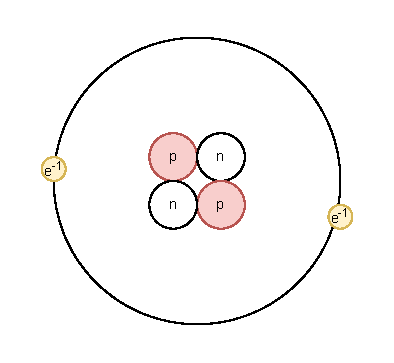
\includegraphics[width=0.5\columnwidth]{fig/helium.pdf}
    \caption{ヘリウム原子の構造}\label{helium-atom}
  \end{figure}
  \begin{myex}{ヘリウム原子の基底エネルギー(荒い近似)}{rough-helium}
    計算を行うと,ヘリウムの原子番号を$Z$として$\hat{H}^0$の基底波動関数,
    \begin{align}
      \psi = \cfrac{Z^3}{\pi a_0^3}\exp\qty(-Z\frac{r_1 + r_2}{a_0})\label{helium}
    \end{align}
    と$\hat{H}^0$の基底エネルギー,
    \begin{align}
      E = -8\ \r{Ry}\approx -108.8\ \r{eV}\label{helium-rough-min}
    \end{align}
    が求まる\footnote{
      $a_0 = \cfrac{4\pi\epsilon_0\hbar^2}{me^2} \approx 5.29\times 10^{-11}\ \r{m}$: Bohr半径
    }\footnote{
      $Z = 2$
    }\footnote{
      $\r{Ry} = \cfrac{\hbar^2}{2m\omega^2} \approx 13.6 \ \r{eV}$: Rydberg定数
    }.
  \end{myex}
  \begin{myex}{ヘリウム原子の基底エネルギー(変分法)}{}
    \exref{rough-helium}の結果とヘリウム原子の基底エネルギーの測定結果は$-78.6\ \r{eV}$と大きく異なっているため,相互作用の項を取り入れた近似を考える.
    \refe{helium}を試行関数$\psi(Z)$とする.
    $\psi(Z)$を用いてエネルギーを計算する.
    \begin{align}
      E(Z) &= \cfrac{\displaystyle\int\psi^{*}\hat{H}\psi \dd{\bm{r}_1}\dd{\bm{r}_2}}{\displaystyle\int\psi^{*}\psi \dd{\bm{r}_1}\dd{\bm{r}_2}} \\
      &= -2\qty(4Z - Z^2 - \cfrac{5}{8}Z)\ \r{Ry}\label{helium-energy-function} 
    \end{align}
    となる.\refe{helium-energy-function}が最小となるような$Z$を$Z_0$とすると$Z_0 = 27/16$であったので,
    \begin{align}
      E(Z) \geq E\qty(Z_0) = -77.5\ \r{eV}\label{helium-energy-varidation-min}
    \end{align}
    となった.\refe{helium-energy-varidation-min}と\refe{helium-rough-min}を比べると,変分法による近似の方が真の基底エネルギ$-78.6\ \r{eV}$に近い値が得られた\footnote{
      $Z_0 < 2$は遮蔽効果により有効電荷が$2e$より小さくなったことを意味する.
    }\footnote{
      積分の計算はDavid J. Griffith, \textit{Introduction to Quantum Mechanics}, pp. 333-334にある.
    }.
  \end{myex}
\end{document}
      \subsection{変分法の誤差の評価}
        \documentclass{report}
\usepackage{luatexja} % LuaTeXで日本語を使うためのパッケージ
\usepackage{luatexja-fontspec} % LuaTeX用の日本語フォント設定

% --- 数学関連 ---
\usepackage{amsmath, amssymb, amsfonts, mathtools, bm, amsthm} % 基本的な数学パッケージ
\usepackage{type1cm, upgreek} % 数式フォントとギリシャ文字
\usepackage{physics, mhchem} % 物理や化学の記号や式の表記を簡単にする

% --- 表関連 ---
\usepackage{multirow, longtable, tabularx, array, colortbl, dcolumn, diagbox} % 表のレイアウトを柔軟にする
\usepackage{tablefootnote, truthtable} % 表中に注釈を追加、真理値表
\usepackage{tabularray} % 高度な表組みレイアウト

% --- グラフィック関連 ---
\usepackage{tikz, graphicx} % 図の描画と画像の挿入
\usepackage{background} % ウォーターマークの設定
\usepackage{caption, subcaption} % 図や表のキャプション設定
\usepackage{float, here} % 図や表の位置指定

% --- レイアウトとページ設定 ---
\usepackage{fancyhdr} % ページヘッダー、フッター、余白の設定
\usepackage[top = 20truemm, bottom = 20truemm, left = 20truemm, right = 20truemm]{geometry}
\usepackage{fancybox, ascmac} % ボックスのデザイン

% --- 色とスタイル ---
\usepackage{xcolor, color, colortbl, tcolorbox} % 色とカラーボックス
\usepackage{listings, jvlisting} % コードの色付けとフォーマット

% --- 参考文献関連 ---
\usepackage{biblatex, usebib} % 参考文献の管理と挿入
\usepackage{url, hyperref} % URLとリンクの設定

% --- その他の便利なパッケージ ---
\usepackage{footmisc} % 脚注のカスタマイズ
\usepackage{multicol} % 複数段組
\usepackage{comment} % コメントアウトの拡張
\usepackage{siunitx} % 単位の表記
\usepackage{docmute}
% \usepackage{appendix}
% --- tcolorboxとtikzの設定 ---
\tcbuselibrary{theorems, breakable} % 定理のボックスと改ページ設定
\usetikzlibrary{decorations.markings, arrows.meta, calc} % tikzの装飾や矢印の設定

% --- 定理スタイルと数式設定 ---
\theoremstyle{definition} % 定義スタイル
\numberwithin{equation}{section} % 式番号をサブセクション単位でリセット

% --- hyperrefの設定 ---
\hypersetup{
  setpagesize = false,
  bookmarks = true,
  bookmarksdepth = tocdepth,
  bookmarksnumbered = true,
  colorlinks = false,
  pdftitle = {}, % PDFタイトル
  pdfsubject = {}, % PDFサブジェクト
  pdfauthor = {}, % PDF作者
  pdfkeywords = {} % PDFキーワード
}

% --- siunitxの設定 ---
\sisetup{
  table-format = 1.5, % 小数点以下の桁数
  table-number-alignment = center, % 数値の中央揃え
}

% --- 透かし画像の設定 --- 
\backgroundsetup{
  scale=0.5,                       % 画像のスケール
  % color=black,                   % 画像の色(透かし用に半透明が推奨)
  opacity=0.2,                   % 透かしの透明度(0が完全透明、1が完全不透明)
  angle=0,                       % 画像の角度
  position = current page.south east,  % ページの右下
  hshift=-6cm, % 右方向へのシフト(負の値で内側に移動)
  vshift=5cm,  % 上方向へのシフト(正の値で内側に移動)
  contents={
\includegraphics{./fig/appilogo-circular-full.png}} % 画像のパス
}

% --- その他の設定 ---
\allowdisplaybreaks % 数式の途中改ページ許可
\newcolumntype{t}{!{\vrule width 0.1pt}} % 新しいカラムタイプ
\newcolumntype{b}{!{\vrule width 1.5pt}} % 太いカラム
\UseTblrLibrary{amsmath, booktabs, counter, diagbox, functional, hook, html, nameref, siunitx, varwidth, zref} % tabularrayのライブラリ
\setlength{\columnseprule}{0.4pt} % カラム区切り線の太さ
\captionsetup[figure]{font = bf} % 図のキャプションの太字設定
\captionsetup[table]{font = bf} % 表のキャプションの太字設定
\captionsetup[lstlisting]{font = bf} % コードのキャプションの太字設定
\captionsetup[subfigure]{font = bf, labelformat = simple} % サブ図のキャプション設定
\setcounter{secnumdepth}{4} % セクションの深さ設定
\newcolumntype{d}{D{.}{.}{5}} % 数値のカラム
\newcolumntype{M}[1]{>{\centering\arraybackslash}m{#1}} % センター揃えのカラム
\DeclareMathOperator{\diag}{diag}
\everymath{\displaystyle} % 数式のスタイル
\newcommand{\inner}[2]{\left\langle #1, #2 \right\rangle}
\renewcommand{\figurename}{図}
\renewcommand{\i}{\mathrm{i}} % 複素数単位i
\renewcommand{\laplacian}{\grad^2} % ラプラシアンの記号
\renewcommand{\thesubfigure}{(\alph{subfigure})} % サブ図の番号形式
\newcommand{\m}[3]{\multicolumn{#1}{#2}{#3}} % マルチカラムのショートカット
\renewcommand{\r}[1]{\mathrm{#1}} % mathrmのショートカット
\newcommand{\e}{\mathrm{e}} % 自然対数の底e
\newcommand{\Ef}{E_{\mathrm{F}}} % フェルミエネルギー
\renewcommand{\c}{\si{\degreeCelsius}} % 摂氏記号
\renewcommand{\d}{\r{d}} % d記号
\renewcommand{\t}[1]{\texttt{#1}} % タイプライタフォント
\newcommand{\kb}{k_{\mathrm{B}}} % ボルツマン定数
% \renewcommand{\phi}{\varphi} % ϕをφに変更
\renewcommand{\epsilon}{\varepsilon}
\newcommand{\fullref}[1]{\textbf{\ref{#1} \nameref{#1}}}
\newcommand{\reff}[1]{\textbf{図\ref{#1}}} % 図参照のショートカット
\newcommand{\reft}[1]{\textbf{表\ref{#1}}} % 表参照のショートカット
\newcommand{\refe}[1]{\textbf{式\eqref{#1}}} % 式参照のショートカット
\newcommand{\refp}[1]{\textbf{コード\ref{#1}}} % コード参照のショートカット
\renewcommand{\lstlistingname}{コード} % コードリストの名前
\renewcommand{\theequation}{\thesection.\arabic{equation}} % 式番号の形式
\renewcommand{\footrulewidth}{0.4pt} % フッターの線
\newcommand{\mar}[1]{\textcircled{\scriptsize #1}} % 丸囲み文字
\newcommand{\combination}[2]{{}_{#1} \mathrm{C}_{#2}} % 組み合わせ
\newcommand{\thline}{\noalign{\hrule height 0.1pt}} % 細い横線
\newcommand{\bhline}{\noalign{\hrule height 1.5pt}} % 太い横線

% --- カスタム色定義 ---
\definecolor{burgundy}{rgb}{0.5, 0.0, 0.13} % バーガンディ色
\definecolor{charcoal}{rgb}{0.21, 0.27, 0.31} % チャコール色
\definecolor{forest}{rgb}{0.0, 0.35, 0} % 森の緑色

% --- カスタム定理環境の定義 ---
\newtcbtheorem[number within = chapter]{myexc}{練習問題}{
  fonttitle = \gtfamily\sffamily\bfseries\upshape,
  colframe = forest,
  colback = forest!2!white,
  rightrule = 1pt,
  leftrule = 1pt,
  bottomrule = 2pt,
  colbacktitle = forest,
  theorem style = standard,
  breakable,
  arc = 0pt,
}{exc-ref}
\newtcbtheorem[number within = chapter]{myprop}{命題}{
  fonttitle = \gtfamily\sffamily\bfseries\upshape,
  colframe = blue!50!black,
  colback = blue!50!black!2!white,
  rightrule = 1pt,
  leftrule = 1pt,
  bottomrule = 2pt,
  colbacktitle = blue!50!black,
  theorem style = standard,
  breakable,
  arc = 0pt
}{proposition-ref}
\newtcbtheorem[number within = chapter]{myrem}{注意}{
  fonttitle = \gtfamily\sffamily\bfseries\upshape,
  colframe = yellow!20!black,
  colback = yellow!50,
  rightrule = 1pt,
  leftrule = 1pt,
  bottomrule = 2pt,
  colbacktitle = yellow!20!black,
  theorem style = standard,
  breakable,
  arc = 0pt
}{remark-ref}
\newtcbtheorem[number within = chapter]{myex}{例題}{
  fonttitle = \gtfamily\sffamily\bfseries\upshape,
  colframe = black,
  colback = white,
  rightrule = 1pt,
  leftrule = 1pt,
  bottomrule = 2pt,
  colbacktitle = black,
  theorem style = standard,
  breakable,
  arc = 0pt
}{example-ref}
\newtcbtheorem[number within = chapter]{exc}{Requirement}{myexc}{exc-ref}
\newcommand{\rqref}[1]{{\bfseries\sffamily 練習問題 \ref{exc-ref:#1}}}
\newtcbtheorem[number within = chapter]{definition}{Definition}{mydef}{definition-ref}
\newcommand{\dfref}[1]{{\bfseries\sffamily 定義 \ref{definition-ref:#1}}}
\newtcbtheorem[number within = chapter]{prop}{命題}{myprop}{proposition-ref}
\newcommand{\prref}[1]{{\bfseries\sffamily 命題 \ref{proposition-ref:#1}}}
\newtcbtheorem[number within = chapter]{rem}{注意}{myrem}{remark-ref}
\newcommand{\rmref}[1]{{\bfseries\sffamily 注意 \ref{remark-ref:#1}}}
\newtcbtheorem[number within = chapter]{ex}{例題}{myex}{example-ref}
\newcommand{\exref}[1]{{\bfseries\sffamily 例題 \ref{example-ref:#1}}}
% --- 再定義コマンド ---
% \mathtoolsset{showonlyrefs=true} % 必要な式番号のみ表示
\pagestyle{fancy} % ヘッダー・フッターのスタイル設定
\chead{応用量子物性講義ノート} % 中央ヘッダー
% \rhead{}
\fancyhead[R]{\rightmark}
\renewcommand{\sectionmark}[1]{\markright{\thesection\ #1}}
\cfoot{\thepage} % 中央フッターにページ番号
\lhead{}
\rfoot{Yuto Masuda and Haruki Aoki} % 右フッターに名前
\setcounter{tocdepth}{4} % 目次の深さ
\makeatletter
\@addtoreset{equation}{section} % サブセクションごとに式番号をリセット
\makeatother

% --- メタ情報 ---
\title{応用量子物性講義ノート}
\date{更新日\today}
\author{Yuto Masuda and Haruki Aoki}

\begin{document}
  真の基底状態$\ket{E_0}$に第1励起状態$\ket{E_1}$を10\%含んだ試行関数$\ket{\psi} = \ket{E_0} + \cfrac{1}{10}\ket{E_1}$を使ってエネルギーを計算する.
  \begin{align}
    E(\psi) &= \frac{\mel{\psi}{\hat{H}}{\psi}}{\braket{\psi}} \\
    &= \cfrac{\bra{E_0}\hat{H}\ket{E_0} + \cfrac{1}{100}\mel{E_1}{\hat{H}}{E_1}}{1 + \cfrac{1}{100}} \\
    &= \cfrac{E_0 + 0.01E_1}{1.01}\\
    &\approx 0.99E_0 + 0.01E_1
  \end{align}
  試行関数で10\%含まれていた誤差がエネルギーでは1\%に収まっている.
  \begin{myex}{}{}
    無限井戸型ポテンシャル$[-a, a]$を考える.
    この問題を厳密に解けば$n$番目のエネルギー準位は,
    \begin{align}
      E_n = \cfrac{\hbar^2}{2m}\qty(\cfrac{n\pi}{2a})^2
    \end{align}
    と計算できるが,ここでは変分法を用いて近似解を求める.
    予想される試行関数の条件は
    \begin{itemize}
      \item $\psi(a) = \psi(-a) = 0$
      \item 節がない
    \end{itemize}
    である.よって今回は
    \begin{align}
      \psi(x) = a^2 - x^2
    \end{align}
    を採用する.この試行関数を用いたときの基底エネルギーを見積もれ.
    \tcblower
    \begin{align}
      E(\psi) &= \cfrac{\displaystyle \int_{-a}^{a}\qty(a^2 - x^2)\qty(-\frac{\hbar^2}{2m}\dv[2]{x})\qty(a^2 - x^2)\dd{x}}{\displaystyle \int_{-a}^{a}\qty(a^2 - x^2)^2\dd{x}} \\
      &= \cfrac{10}{\pi^2}E_1 \\
      &\approx 1.01E_1
    \end{align}
    真の基底エネルギー$E_1$に近い値が得られた\footnote{このくらいの計算が期末試験に出たことがある.}.
  \end{myex}
\end{document}
      \subsection{練習問題}
        \documentclass{report}
\usepackage{luatexja} % LuaTeXで日本語を使うためのパッケージ
\usepackage{luatexja-fontspec} % LuaTeX用の日本語フォント設定

% --- 数学関連 ---
\usepackage{amsmath, amssymb, amsfonts, mathtools, bm, amsthm} % 基本的な数学パッケージ
\usepackage{type1cm, upgreek} % 数式フォントとギリシャ文字
\usepackage{physics, mhchem} % 物理や化学の記号や式の表記を簡単にする

% --- 表関連 ---
\usepackage{multirow, longtable, tabularx, array, colortbl, dcolumn, diagbox} % 表のレイアウトを柔軟にする
\usepackage{tablefootnote, truthtable} % 表中に注釈を追加、真理値表
\usepackage{tabularray} % 高度な表組みレイアウト

% --- グラフィック関連 ---
\usepackage{tikz, graphicx} % 図の描画と画像の挿入
\usepackage{background} % ウォーターマークの設定
\usepackage{caption, subcaption} % 図や表のキャプション設定
\usepackage{float, here} % 図や表の位置指定

% --- レイアウトとページ設定 ---
\usepackage{fancyhdr} % ページヘッダー、フッター、余白の設定
\usepackage[top = 20truemm, bottom = 20truemm, left = 20truemm, right = 20truemm]{geometry}
\usepackage{fancybox, ascmac} % ボックスのデザイン

% --- 色とスタイル ---
\usepackage{xcolor, color, colortbl, tcolorbox} % 色とカラーボックス
\usepackage{listings, jvlisting} % コードの色付けとフォーマット

% --- 参考文献関連 ---
\usepackage{biblatex, usebib} % 参考文献の管理と挿入
\usepackage{url, hyperref} % URLとリンクの設定

% --- その他の便利なパッケージ ---
\usepackage{footmisc} % 脚注のカスタマイズ
\usepackage{multicol} % 複数段組
\usepackage{comment} % コメントアウトの拡張
\usepackage{siunitx} % 単位の表記
\usepackage{docmute}
% \usepackage{appendix}
% --- tcolorboxとtikzの設定 ---
\tcbuselibrary{theorems, breakable} % 定理のボックスと改ページ設定
\usetikzlibrary{decorations.markings, arrows.meta, calc} % tikzの装飾や矢印の設定

% --- 定理スタイルと数式設定 ---
\theoremstyle{definition} % 定義スタイル
\numberwithin{equation}{section} % 式番号をサブセクション単位でリセット

% --- hyperrefの設定 ---
\hypersetup{
  setpagesize = false,
  bookmarks = true,
  bookmarksdepth = tocdepth,
  bookmarksnumbered = true,
  colorlinks = false,
  pdftitle = {}, % PDFタイトル
  pdfsubject = {}, % PDFサブジェクト
  pdfauthor = {}, % PDF作者
  pdfkeywords = {} % PDFキーワード
}

% --- siunitxの設定 ---
\sisetup{
  table-format = 1.5, % 小数点以下の桁数
  table-number-alignment = center, % 数値の中央揃え
}

% --- 透かし画像の設定 --- 
\backgroundsetup{
  scale=0.5,                       % 画像のスケール
  % color=black,                   % 画像の色(透かし用に半透明が推奨)
  opacity=0.2,                   % 透かしの透明度(0が完全透明、1が完全不透明)
  angle=0,                       % 画像の角度
  position = current page.south east,  % ページの右下
  hshift=-6cm, % 右方向へのシフト(負の値で内側に移動)
  vshift=5cm,  % 上方向へのシフト(正の値で内側に移動)
  contents={
\includegraphics{./fig/appilogo-circular-full.png}} % 画像のパス
}

% --- その他の設定 ---
\allowdisplaybreaks % 数式の途中改ページ許可
\newcolumntype{t}{!{\vrule width 0.1pt}} % 新しいカラムタイプ
\newcolumntype{b}{!{\vrule width 1.5pt}} % 太いカラム
\UseTblrLibrary{amsmath, booktabs, counter, diagbox, functional, hook, html, nameref, siunitx, varwidth, zref} % tabularrayのライブラリ
\setlength{\columnseprule}{0.4pt} % カラム区切り線の太さ
\captionsetup[figure]{font = bf} % 図のキャプションの太字設定
\captionsetup[table]{font = bf} % 表のキャプションの太字設定
\captionsetup[lstlisting]{font = bf} % コードのキャプションの太字設定
\captionsetup[subfigure]{font = bf, labelformat = simple} % サブ図のキャプション設定
\setcounter{secnumdepth}{4} % セクションの深さ設定
\newcolumntype{d}{D{.}{.}{5}} % 数値のカラム
\newcolumntype{M}[1]{>{\centering\arraybackslash}m{#1}} % センター揃えのカラム
\DeclareMathOperator{\diag}{diag}
\everymath{\displaystyle} % 数式のスタイル
\newcommand{\inner}[2]{\left\langle #1, #2 \right\rangle}
\renewcommand{\figurename}{図}
\renewcommand{\i}{\mathrm{i}} % 複素数単位i
\renewcommand{\laplacian}{\grad^2} % ラプラシアンの記号
\renewcommand{\thesubfigure}{(\alph{subfigure})} % サブ図の番号形式
\newcommand{\m}[3]{\multicolumn{#1}{#2}{#3}} % マルチカラムのショートカット
\renewcommand{\r}[1]{\mathrm{#1}} % mathrmのショートカット
\newcommand{\e}{\mathrm{e}} % 自然対数の底e
\newcommand{\Ef}{E_{\mathrm{F}}} % フェルミエネルギー
\renewcommand{\c}{\si{\degreeCelsius}} % 摂氏記号
\renewcommand{\d}{\r{d}} % d記号
\renewcommand{\t}[1]{\texttt{#1}} % タイプライタフォント
\newcommand{\kb}{k_{\mathrm{B}}} % ボルツマン定数
% \renewcommand{\phi}{\varphi} % ϕをφに変更
\renewcommand{\epsilon}{\varepsilon}
\newcommand{\fullref}[1]{\textbf{\ref{#1} \nameref{#1}}}
\newcommand{\reff}[1]{\textbf{図\ref{#1}}} % 図参照のショートカット
\newcommand{\reft}[1]{\textbf{表\ref{#1}}} % 表参照のショートカット
\newcommand{\refe}[1]{\textbf{式\eqref{#1}}} % 式参照のショートカット
\newcommand{\refp}[1]{\textbf{コード\ref{#1}}} % コード参照のショートカット
\renewcommand{\lstlistingname}{コード} % コードリストの名前
\renewcommand{\theequation}{\thesection.\arabic{equation}} % 式番号の形式
\renewcommand{\footrulewidth}{0.4pt} % フッターの線
\newcommand{\mar}[1]{\textcircled{\scriptsize #1}} % 丸囲み文字
\newcommand{\combination}[2]{{}_{#1} \mathrm{C}_{#2}} % 組み合わせ
\newcommand{\thline}{\noalign{\hrule height 0.1pt}} % 細い横線
\newcommand{\bhline}{\noalign{\hrule height 1.5pt}} % 太い横線

% --- カスタム色定義 ---
\definecolor{burgundy}{rgb}{0.5, 0.0, 0.13} % バーガンディ色
\definecolor{charcoal}{rgb}{0.21, 0.27, 0.31} % チャコール色
\definecolor{forest}{rgb}{0.0, 0.35, 0} % 森の緑色

% --- カスタム定理環境の定義 ---
\newtcbtheorem[number within = chapter]{myexc}{練習問題}{
  fonttitle = \gtfamily\sffamily\bfseries\upshape,
  colframe = forest,
  colback = forest!2!white,
  rightrule = 1pt,
  leftrule = 1pt,
  bottomrule = 2pt,
  colbacktitle = forest,
  theorem style = standard,
  breakable,
  arc = 0pt,
}{exc-ref}
\newtcbtheorem[number within = chapter]{myprop}{命題}{
  fonttitle = \gtfamily\sffamily\bfseries\upshape,
  colframe = blue!50!black,
  colback = blue!50!black!2!white,
  rightrule = 1pt,
  leftrule = 1pt,
  bottomrule = 2pt,
  colbacktitle = blue!50!black,
  theorem style = standard,
  breakable,
  arc = 0pt
}{proposition-ref}
\newtcbtheorem[number within = chapter]{myrem}{注意}{
  fonttitle = \gtfamily\sffamily\bfseries\upshape,
  colframe = yellow!20!black,
  colback = yellow!50,
  rightrule = 1pt,
  leftrule = 1pt,
  bottomrule = 2pt,
  colbacktitle = yellow!20!black,
  theorem style = standard,
  breakable,
  arc = 0pt
}{remark-ref}
\newtcbtheorem[number within = chapter]{myex}{例題}{
  fonttitle = \gtfamily\sffamily\bfseries\upshape,
  colframe = black,
  colback = white,
  rightrule = 1pt,
  leftrule = 1pt,
  bottomrule = 2pt,
  colbacktitle = black,
  theorem style = standard,
  breakable,
  arc = 0pt
}{example-ref}
\newtcbtheorem[number within = chapter]{exc}{Requirement}{myexc}{exc-ref}
\newcommand{\rqref}[1]{{\bfseries\sffamily 練習問題 \ref{exc-ref:#1}}}
\newtcbtheorem[number within = chapter]{definition}{Definition}{mydef}{definition-ref}
\newcommand{\dfref}[1]{{\bfseries\sffamily 定義 \ref{definition-ref:#1}}}
\newtcbtheorem[number within = chapter]{prop}{命題}{myprop}{proposition-ref}
\newcommand{\prref}[1]{{\bfseries\sffamily 命題 \ref{proposition-ref:#1}}}
\newtcbtheorem[number within = chapter]{rem}{注意}{myrem}{remark-ref}
\newcommand{\rmref}[1]{{\bfseries\sffamily 注意 \ref{remark-ref:#1}}}
\newtcbtheorem[number within = chapter]{ex}{例題}{myex}{example-ref}
\newcommand{\exref}[1]{{\bfseries\sffamily 例題 \ref{example-ref:#1}}}
% --- 再定義コマンド ---
% \mathtoolsset{showonlyrefs=true} % 必要な式番号のみ表示
\pagestyle{fancy} % ヘッダー・フッターのスタイル設定
\chead{応用量子物性講義ノート} % 中央ヘッダー
% \rhead{}
\fancyhead[R]{\rightmark}
\renewcommand{\sectionmark}[1]{\markright{\thesection\ #1}}
\cfoot{\thepage} % 中央フッターにページ番号
\lhead{}
\rfoot{Yuto Masuda and Haruki Aoki} % 右フッターに名前
\setcounter{tocdepth}{4} % 目次の深さ
\makeatletter
\@addtoreset{equation}{section} % サブセクションごとに式番号をリセット
\makeatother

% --- メタ情報 ---
\title{応用量子物性講義ノート}
\date{更新日\today}
\author{Yuto Masuda and Haruki Aoki}

\begin{document}
  \begin{myexc}{Griffith Example 8.1}{}
    1次元調和振動子$\hat{H} = -\cfrac{\hbar^2}{2m}\dv[2]{x} + \cfrac{1}{2}m\omega^2 x^2$の基底エネルギーを見積もれ.
    ただし,試行関数を$\psi(x) = \qty(\cfrac{2b}{\pi})^{1/4}\e^{-bx^2}$とせよ.試行関数は規格化されている.
    \tcblower
    \begin{align}
      E(b) = \bra{\psi}\hat{H}\ket{\psi} &= \qty(\cfrac{2b}{\pi})^{1/2}\int_{-\infty}^{\infty}\e^{-bx^2}\qty(-\cfrac{\hbar^2}{2m}\dv[2]{x} + \cfrac{1}{2}m\omega^2x^2)\e^{-bx^2}\dd{x}\\
      &=\cfrac{\hbar^2b}{2m}+\cfrac{m\omega^2}{8b}
    \end{align}
    次に$E(b)$の最小値を求める.
    \begin{align}
      \dv{b}E(b_0) = \cfrac{\hbar^2}{2m} - \cfrac{m\omega^2}{8b_{0}^2} = 0\Rightarrow b_0 = \cfrac{m\omega}{2\hbar}
    \end{align}
    \begin{align}
      E(b_0) = \cfrac{1}{2}\hbar\omega
    \end{align}
    偶然にも試行関数は基底エネルギーの固有関数となっていたため,$E(b_0)$は基底エネルギーと一致した.
  \end{myexc}
  \begin{myexc}{Griffith Example 8.2}{}
    デルタ関数型ポテンシャル$\hat{H} - \dv[2]{x}-\alpha \delta(x)$の基底エネルギーを見積もれ.
    ただし,試行関数を$\psi(x) = \qty(\cfrac{2b}{\pi})^{1/4}\e^{-bx^2}$とせよ.試行関数は規格化されている.
    \tcblower
    \begin{align}
      \ev{V} &= -\alpha \qty(\cfrac{2b}{\pi})^{1/2}\int_{-\infty}^{\infty}\e^{-2bx^2}\delta(x)\dd{x} = -\alpha\qty(\cfrac{2b}{\pi})^{1/2}\\
      \ev{T} &= \cfrac{\hbar^2 b}{2m}\\
      E(b) &= \cfrac{\hbar^2 b}{2m} - \alpha\qty(\cfrac{2b}{\pi})^{1/2}
    \end{align}
    $E(b)$の最小値を求める.
    \begin{align}
      \dv{b}E(b_0) = \cfrac{\hbar^2}{2m} - \cfrac{\alpha}{\sqrt{2\pi b_0}} = 0\Rightarrow b_0=\cfrac{2m^2\alpha^2}{\pi\hbar^4}
    \end{align}
    よって,基底エネルギーの近似解として
    \begin{align}
      E(b_0) = -\cfrac{m\alpha^2}{\pi\hbar^2}
    \end{align}
    を得る\footnote{
      厳密解を求めることができ,$\psi(x) = \cfrac{\sqrt{m\alpha}}{\hbar}\e^{-m\alpha\abs{x}/\hbar^2},\ E_0 = -\cfrac{m\alpha^2}{2\hbar^2}$である.
    }.
  \end{myexc}
  \begin{myexc}{Griffith Example 8.3}{}
    $[0, a]$の無限井戸型ポテンシャルの基底エネルギーを見積もれ.ただし,試行関数を
    \begin{align}
      \psi(x)=
      \begin{dcases*}
        Ax & if $0 \leq x \leq a/2$ \\
        A(a - x) & if $a/2\leq x \leq a$ \\ 
        0 & otherwise 
      \end{dcases*}
    \end{align}
    とせよ.
    \tcblower
    規格化条件より,$A = \cfrac{2}{a}\sqrt{\cfrac{3}{a}}$を得る.波動関数の導関数は
    \begin{align}
      \dv[2]{\psi}{x} =
        \begin{dcases*}
          Ax & if $0 \leq x \leq a/2$ \\
          A(a - x) & if $a/2\leq x \leq a$ \\ 
          0 & otherwise 
        \end{dcases*}
    \end{align}
    である.よって,2次の微係数として
    \begin{align}
      \dv[2]{\psi}{x} = A\delta(x) - 2A\delta\qty(x - \cfrac{a}{2}) + A\delta(x - a)
    \end{align}
    を得る.したがって近似解は
    \begin{align}
      E &= \int_{0}^{a}\psi(x)\qty(-\cfrac{\hbar^2}{2m}\dv[2]{x})\psi(x)\dd{x}\\
      &= -\cfrac{\hbar^2}{2m}\int_{0}^{a} A\qty[\delta(x)-\delta\qty(x-\cfrac{a}{2}) + \delta(x - a)]\psi(x)\dd{x}\\
      &= \cfrac{12\hbar^2}{2ma^2}
    \end{align}
    である\footnote{
      厳密解は$E_0 = \cfrac{\pi^2\hbar^2}{2ma^2}$
    }.
  \end{myexc}
  \begin{myexc}{Griffith Problem8.4 (a)}{}
    試行関数$\ket{\psi}$が基底状態と直交するとき,つまり$\braket{\psi}{0}$のとき,
    \begin{align}
      E(\psi)\geq E_1
    \end{align}
    であることを示せ\footnote{
      例えば偶関数のポテンシャルに対し奇関数の試行関数で計算すれば第1励起状態のエネルギーの近似解が得られる.
    }.
    ただし$E_1$は第1励起状態のエネルギーである.$\ket{\psi}$は規格化されている.
    \tcblower
    \begin{proof}
      \begin{align}
        E(\psi) &= \sum_{k = 0}E_k\abs{\braket{\psi}{k}}^2 \\
        &= E_0\abs{\braket{\psi}{0}}^2 + \sum_{k = 1}\abs{\braket{\psi}{k}}^2 \\
        &= 0 + \sum_{k = 1}\abs{\braket{\psi}{k}}^2 \\
        &\geq E_1\sum_{k = 1}\abs{\braket{\psi}{k}}^2 = E_1
      \end{align}
    \end{proof}
  \end{myexc}
\end{document}

    \section{摂動I(定常摂動)}
      \documentclass{standalone}
\usepackage{luatexja} % LuaTeXで日本語を使うためのパッケージ
\usepackage{luatexja-fontspec} % LuaTeX用の日本語フォント設定

% --- 数学関連 ---
\usepackage{amsmath, amssymb, amsfonts, mathtools, bm, amsthm} % 基本的な数学パッケージ
\usepackage{type1cm, upgreek} % 数式フォントとギリシャ文字
\usepackage{physics, mhchem} % 物理や化学の記号や式の表記を簡単にする

% --- 表関連 ---
\usepackage{multirow, longtable, tabularx, array, colortbl, dcolumn, diagbox} % 表のレイアウトを柔軟にする
\usepackage{tablefootnote, truthtable} % 表中に注釈を追加、真理値表
\usepackage{tabularray} % 高度な表組みレイアウト

% --- グラフィック関連 ---
\usepackage{tikz, graphicx} % 図の描画と画像の挿入
\usepackage{background} % ウォーターマークの設定
\usepackage{caption, subcaption} % 図や表のキャプション設定
\usepackage{float, here} % 図や表の位置指定

% --- レイアウトとページ設定 ---
\usepackage{fancyhdr} % ページヘッダー、フッター、余白の設定
\usepackage[top = 20truemm, bottom = 20truemm, left = 20truemm, right = 20truemm]{geometry}
\usepackage{fancybox, ascmac} % ボックスのデザイン

% --- 色とスタイル ---
\usepackage{xcolor, color, colortbl, tcolorbox} % 色とカラーボックス
\usepackage{listings, jvlisting} % コードの色付けとフォーマット

% --- 参考文献関連 ---
\usepackage{biblatex, usebib} % 参考文献の管理と挿入
\usepackage{url, hyperref} % URLとリンクの設定

% --- その他の便利なパッケージ ---
\usepackage{footmisc} % 脚注のカスタマイズ
\usepackage{multicol} % 複数段組
\usepackage{comment} % コメントアウトの拡張
\usepackage{siunitx} % 単位の表記
\usepackage{docmute}
% \usepackage{appendix}
% --- tcolorboxとtikzの設定 ---
\tcbuselibrary{theorems, breakable} % 定理のボックスと改ページ設定
\usetikzlibrary{decorations.markings, arrows.meta, calc} % tikzの装飾や矢印の設定

% --- 定理スタイルと数式設定 ---
\theoremstyle{definition} % 定義スタイル
\numberwithin{equation}{section} % 式番号をサブセクション単位でリセット

% --- hyperrefの設定 ---
\hypersetup{
  setpagesize = false,
  bookmarks = true,
  bookmarksdepth = tocdepth,
  bookmarksnumbered = true,
  colorlinks = false,
  pdftitle = {}, % PDFタイトル
  pdfsubject = {}, % PDFサブジェクト
  pdfauthor = {}, % PDF作者
  pdfkeywords = {} % PDFキーワード
}

% --- siunitxの設定 ---
\sisetup{
  table-format = 1.5, % 小数点以下の桁数
  table-number-alignment = center, % 数値の中央揃え
}

% --- 透かし画像の設定 --- 
\backgroundsetup{
  scale=0.5,                       % 画像のスケール
  % color=black,                   % 画像の色(透かし用に半透明が推奨)
  opacity=0.2,                   % 透かしの透明度(0が完全透明、1が完全不透明)
  angle=0,                       % 画像の角度
  position = current page.south east,  % ページの右下
  hshift=-6cm, % 右方向へのシフト(負の値で内側に移動)
  vshift=5cm,  % 上方向へのシフト(正の値で内側に移動)
  contents={
\includegraphics{./fig/appilogo-circular-full.png}} % 画像のパス
}

% --- その他の設定 ---
\allowdisplaybreaks % 数式の途中改ページ許可
\newcolumntype{t}{!{\vrule width 0.1pt}} % 新しいカラムタイプ
\newcolumntype{b}{!{\vrule width 1.5pt}} % 太いカラム
\UseTblrLibrary{amsmath, booktabs, counter, diagbox, functional, hook, html, nameref, siunitx, varwidth, zref} % tabularrayのライブラリ
\setlength{\columnseprule}{0.4pt} % カラム区切り線の太さ
\captionsetup[figure]{font = bf} % 図のキャプションの太字設定
\captionsetup[table]{font = bf} % 表のキャプションの太字設定
\captionsetup[lstlisting]{font = bf} % コードのキャプションの太字設定
\captionsetup[subfigure]{font = bf, labelformat = simple} % サブ図のキャプション設定
\setcounter{secnumdepth}{4} % セクションの深さ設定
\newcolumntype{d}{D{.}{.}{5}} % 数値のカラム
\newcolumntype{M}[1]{>{\centering\arraybackslash}m{#1}} % センター揃えのカラム
\DeclareMathOperator{\diag}{diag}
\everymath{\displaystyle} % 数式のスタイル
\newcommand{\inner}[2]{\left\langle #1, #2 \right\rangle}
\renewcommand{\figurename}{図}
\renewcommand{\i}{\mathrm{i}} % 複素数単位i
\renewcommand{\laplacian}{\grad^2} % ラプラシアンの記号
\renewcommand{\thesubfigure}{(\alph{subfigure})} % サブ図の番号形式
\newcommand{\m}[3]{\multicolumn{#1}{#2}{#3}} % マルチカラムのショートカット
\renewcommand{\r}[1]{\mathrm{#1}} % mathrmのショートカット
\newcommand{\e}{\mathrm{e}} % 自然対数の底e
\newcommand{\Ef}{E_{\mathrm{F}}} % フェルミエネルギー
\renewcommand{\c}{\si{\degreeCelsius}} % 摂氏記号
\renewcommand{\d}{\r{d}} % d記号
\renewcommand{\t}[1]{\texttt{#1}} % タイプライタフォント
\newcommand{\kb}{k_{\mathrm{B}}} % ボルツマン定数
% \renewcommand{\phi}{\varphi} % ϕをφに変更
\renewcommand{\epsilon}{\varepsilon}
\newcommand{\fullref}[1]{\textbf{\ref{#1} \nameref{#1}}}
\newcommand{\reff}[1]{\textbf{図\ref{#1}}} % 図参照のショートカット
\newcommand{\reft}[1]{\textbf{表\ref{#1}}} % 表参照のショートカット
\newcommand{\refe}[1]{\textbf{式\eqref{#1}}} % 式参照のショートカット
\newcommand{\refp}[1]{\textbf{コード\ref{#1}}} % コード参照のショートカット
\renewcommand{\lstlistingname}{コード} % コードリストの名前
\renewcommand{\theequation}{\thesection.\arabic{equation}} % 式番号の形式
\renewcommand{\footrulewidth}{0.4pt} % フッターの線
\newcommand{\mar}[1]{\textcircled{\scriptsize #1}} % 丸囲み文字
\newcommand{\combination}[2]{{}_{#1} \mathrm{C}_{#2}} % 組み合わせ
\newcommand{\thline}{\noalign{\hrule height 0.1pt}} % 細い横線
\newcommand{\bhline}{\noalign{\hrule height 1.5pt}} % 太い横線

% --- カスタム色定義 ---
\definecolor{burgundy}{rgb}{0.5, 0.0, 0.13} % バーガンディ色
\definecolor{charcoal}{rgb}{0.21, 0.27, 0.31} % チャコール色
\definecolor{forest}{rgb}{0.0, 0.35, 0} % 森の緑色

% --- カスタム定理環境の定義 ---
\newtcbtheorem[number within = chapter]{myexc}{練習問題}{
  fonttitle = \gtfamily\sffamily\bfseries\upshape,
  colframe = forest,
  colback = forest!2!white,
  rightrule = 1pt,
  leftrule = 1pt,
  bottomrule = 2pt,
  colbacktitle = forest,
  theorem style = standard,
  breakable,
  arc = 0pt,
}{exc-ref}
\newtcbtheorem[number within = chapter]{myprop}{命題}{
  fonttitle = \gtfamily\sffamily\bfseries\upshape,
  colframe = blue!50!black,
  colback = blue!50!black!2!white,
  rightrule = 1pt,
  leftrule = 1pt,
  bottomrule = 2pt,
  colbacktitle = blue!50!black,
  theorem style = standard,
  breakable,
  arc = 0pt
}{proposition-ref}
\newtcbtheorem[number within = chapter]{myrem}{注意}{
  fonttitle = \gtfamily\sffamily\bfseries\upshape,
  colframe = yellow!20!black,
  colback = yellow!50,
  rightrule = 1pt,
  leftrule = 1pt,
  bottomrule = 2pt,
  colbacktitle = yellow!20!black,
  theorem style = standard,
  breakable,
  arc = 0pt
}{remark-ref}
\newtcbtheorem[number within = chapter]{myex}{例題}{
  fonttitle = \gtfamily\sffamily\bfseries\upshape,
  colframe = black,
  colback = white,
  rightrule = 1pt,
  leftrule = 1pt,
  bottomrule = 2pt,
  colbacktitle = black,
  theorem style = standard,
  breakable,
  arc = 0pt
}{example-ref}
\newtcbtheorem[number within = chapter]{exc}{Requirement}{myexc}{exc-ref}
\newcommand{\rqref}[1]{{\bfseries\sffamily 練習問題 \ref{exc-ref:#1}}}
\newtcbtheorem[number within = chapter]{definition}{Definition}{mydef}{definition-ref}
\newcommand{\dfref}[1]{{\bfseries\sffamily 定義 \ref{definition-ref:#1}}}
\newtcbtheorem[number within = chapter]{prop}{命題}{myprop}{proposition-ref}
\newcommand{\prref}[1]{{\bfseries\sffamily 命題 \ref{proposition-ref:#1}}}
\newtcbtheorem[number within = chapter]{rem}{注意}{myrem}{remark-ref}
\newcommand{\rmref}[1]{{\bfseries\sffamily 注意 \ref{remark-ref:#1}}}
\newtcbtheorem[number within = chapter]{ex}{例題}{myex}{example-ref}
\newcommand{\exref}[1]{{\bfseries\sffamily 例題 \ref{example-ref:#1}}}
% --- 再定義コマンド ---
% \mathtoolsset{showonlyrefs=true} % 必要な式番号のみ表示
\pagestyle{fancy} % ヘッダー・フッターのスタイル設定
\chead{応用量子物性講義ノート} % 中央ヘッダー
% \rhead{}
\fancyhead[R]{\rightmark}
\renewcommand{\sectionmark}[1]{\markright{\thesection\ #1}}
\cfoot{\thepage} % 中央フッターにページ番号
\lhead{}
\rfoot{Yuto Masuda and Haruki Aoki} % 右フッターに名前
\setcounter{tocdepth}{4} % 目次の深さ
\makeatletter
\@addtoreset{equation}{section} % サブセクションごとに式番号をリセット
\makeatother

% --- メタ情報 ---
\title{応用量子物性講義ノート}
\date{更新日\today}
\author{Yuto Masuda and Haruki Aoki}

\begin{document}
  Hamiltonianが時間に依存しない定常摂動(time-independent perturbation)を扱う.
\end{document}

      \subsection{準備}
        \documentclass{report}
\usepackage{luatexja} % LuaTeXで日本語を使うためのパッケージ
\usepackage{luatexja-fontspec} % LuaTeX用の日本語フォント設定

% --- 数学関連 ---
\usepackage{amsmath, amssymb, amsfonts, mathtools, bm, amsthm} % 基本的な数学パッケージ
\usepackage{type1cm, upgreek} % 数式フォントとギリシャ文字
\usepackage{physics, mhchem} % 物理や化学の記号や式の表記を簡単にする

% --- 表関連 ---
\usepackage{multirow, longtable, tabularx, array, colortbl, dcolumn, diagbox} % 表のレイアウトを柔軟にする
\usepackage{tablefootnote, truthtable} % 表中に注釈を追加、真理値表
\usepackage{tabularray} % 高度な表組みレイアウト

% --- グラフィック関連 ---
\usepackage{tikz, graphicx} % 図の描画と画像の挿入
\usepackage{background} % ウォーターマークの設定
\usepackage{caption, subcaption} % 図や表のキャプション設定
\usepackage{float, here} % 図や表の位置指定

% --- レイアウトとページ設定 ---
\usepackage{fancyhdr} % ページヘッダー、フッター、余白の設定
\usepackage[top = 20truemm, bottom = 20truemm, left = 20truemm, right = 20truemm]{geometry}
\usepackage{fancybox, ascmac} % ボックスのデザイン

% --- 色とスタイル ---
\usepackage{xcolor, color, colortbl, tcolorbox} % 色とカラーボックス
\usepackage{listings, jvlisting} % コードの色付けとフォーマット

% --- 参考文献関連 ---
\usepackage{biblatex, usebib} % 参考文献の管理と挿入
\usepackage{url, hyperref} % URLとリンクの設定

% --- その他の便利なパッケージ ---
\usepackage{footmisc} % 脚注のカスタマイズ
\usepackage{multicol} % 複数段組
\usepackage{comment} % コメントアウトの拡張
\usepackage{siunitx} % 単位の表記
\usepackage{docmute}
% \usepackage{appendix}
% --- tcolorboxとtikzの設定 ---
\tcbuselibrary{theorems, breakable} % 定理のボックスと改ページ設定
\usetikzlibrary{decorations.markings, arrows.meta, calc} % tikzの装飾や矢印の設定

% --- 定理スタイルと数式設定 ---
\theoremstyle{definition} % 定義スタイル
\numberwithin{equation}{section} % 式番号をサブセクション単位でリセット

% --- hyperrefの設定 ---
\hypersetup{
  setpagesize = false,
  bookmarks = true,
  bookmarksdepth = tocdepth,
  bookmarksnumbered = true,
  colorlinks = false,
  pdftitle = {}, % PDFタイトル
  pdfsubject = {}, % PDFサブジェクト
  pdfauthor = {}, % PDF作者
  pdfkeywords = {} % PDFキーワード
}

% --- siunitxの設定 ---
\sisetup{
  table-format = 1.5, % 小数点以下の桁数
  table-number-alignment = center, % 数値の中央揃え
}

% --- 透かし画像の設定 --- 
\backgroundsetup{
  scale=0.5,                       % 画像のスケール
  % color=black,                   % 画像の色(透かし用に半透明が推奨)
  opacity=0.2,                   % 透かしの透明度(0が完全透明、1が完全不透明)
  angle=0,                       % 画像の角度
  position = current page.south east,  % ページの右下
  hshift=-6cm, % 右方向へのシフト(負の値で内側に移動)
  vshift=5cm,  % 上方向へのシフト(正の値で内側に移動)
  contents={
\includegraphics{./fig/appilogo-circular-full.png}} % 画像のパス
}

% --- その他の設定 ---
\allowdisplaybreaks % 数式の途中改ページ許可
\newcolumntype{t}{!{\vrule width 0.1pt}} % 新しいカラムタイプ
\newcolumntype{b}{!{\vrule width 1.5pt}} % 太いカラム
\UseTblrLibrary{amsmath, booktabs, counter, diagbox, functional, hook, html, nameref, siunitx, varwidth, zref} % tabularrayのライブラリ
\setlength{\columnseprule}{0.4pt} % カラム区切り線の太さ
\captionsetup[figure]{font = bf} % 図のキャプションの太字設定
\captionsetup[table]{font = bf} % 表のキャプションの太字設定
\captionsetup[lstlisting]{font = bf} % コードのキャプションの太字設定
\captionsetup[subfigure]{font = bf, labelformat = simple} % サブ図のキャプション設定
\setcounter{secnumdepth}{4} % セクションの深さ設定
\newcolumntype{d}{D{.}{.}{5}} % 数値のカラム
\newcolumntype{M}[1]{>{\centering\arraybackslash}m{#1}} % センター揃えのカラム
\DeclareMathOperator{\diag}{diag}
\everymath{\displaystyle} % 数式のスタイル
\newcommand{\inner}[2]{\left\langle #1, #2 \right\rangle}
\renewcommand{\figurename}{図}
\renewcommand{\i}{\mathrm{i}} % 複素数単位i
\renewcommand{\laplacian}{\grad^2} % ラプラシアンの記号
\renewcommand{\thesubfigure}{(\alph{subfigure})} % サブ図の番号形式
\newcommand{\m}[3]{\multicolumn{#1}{#2}{#3}} % マルチカラムのショートカット
\renewcommand{\r}[1]{\mathrm{#1}} % mathrmのショートカット
\newcommand{\e}{\mathrm{e}} % 自然対数の底e
\newcommand{\Ef}{E_{\mathrm{F}}} % フェルミエネルギー
\renewcommand{\c}{\si{\degreeCelsius}} % 摂氏記号
\renewcommand{\d}{\r{d}} % d記号
\renewcommand{\t}[1]{\texttt{#1}} % タイプライタフォント
\newcommand{\kb}{k_{\mathrm{B}}} % ボルツマン定数
% \renewcommand{\phi}{\varphi} % ϕをφに変更
\renewcommand{\epsilon}{\varepsilon}
\newcommand{\fullref}[1]{\textbf{\ref{#1} \nameref{#1}}}
\newcommand{\reff}[1]{\textbf{図\ref{#1}}} % 図参照のショートカット
\newcommand{\reft}[1]{\textbf{表\ref{#1}}} % 表参照のショートカット
\newcommand{\refe}[1]{\textbf{式\eqref{#1}}} % 式参照のショートカット
\newcommand{\refp}[1]{\textbf{コード\ref{#1}}} % コード参照のショートカット
\renewcommand{\lstlistingname}{コード} % コードリストの名前
\renewcommand{\theequation}{\thesection.\arabic{equation}} % 式番号の形式
\renewcommand{\footrulewidth}{0.4pt} % フッターの線
\newcommand{\mar}[1]{\textcircled{\scriptsize #1}} % 丸囲み文字
\newcommand{\combination}[2]{{}_{#1} \mathrm{C}_{#2}} % 組み合わせ
\newcommand{\thline}{\noalign{\hrule height 0.1pt}} % 細い横線
\newcommand{\bhline}{\noalign{\hrule height 1.5pt}} % 太い横線

% --- カスタム色定義 ---
\definecolor{burgundy}{rgb}{0.5, 0.0, 0.13} % バーガンディ色
\definecolor{charcoal}{rgb}{0.21, 0.27, 0.31} % チャコール色
\definecolor{forest}{rgb}{0.0, 0.35, 0} % 森の緑色

% --- カスタム定理環境の定義 ---
\newtcbtheorem[number within = chapter]{myexc}{練習問題}{
  fonttitle = \gtfamily\sffamily\bfseries\upshape,
  colframe = forest,
  colback = forest!2!white,
  rightrule = 1pt,
  leftrule = 1pt,
  bottomrule = 2pt,
  colbacktitle = forest,
  theorem style = standard,
  breakable,
  arc = 0pt,
}{exc-ref}
\newtcbtheorem[number within = chapter]{myprop}{命題}{
  fonttitle = \gtfamily\sffamily\bfseries\upshape,
  colframe = blue!50!black,
  colback = blue!50!black!2!white,
  rightrule = 1pt,
  leftrule = 1pt,
  bottomrule = 2pt,
  colbacktitle = blue!50!black,
  theorem style = standard,
  breakable,
  arc = 0pt
}{proposition-ref}
\newtcbtheorem[number within = chapter]{myrem}{注意}{
  fonttitle = \gtfamily\sffamily\bfseries\upshape,
  colframe = yellow!20!black,
  colback = yellow!50,
  rightrule = 1pt,
  leftrule = 1pt,
  bottomrule = 2pt,
  colbacktitle = yellow!20!black,
  theorem style = standard,
  breakable,
  arc = 0pt
}{remark-ref}
\newtcbtheorem[number within = chapter]{myex}{例題}{
  fonttitle = \gtfamily\sffamily\bfseries\upshape,
  colframe = black,
  colback = white,
  rightrule = 1pt,
  leftrule = 1pt,
  bottomrule = 2pt,
  colbacktitle = black,
  theorem style = standard,
  breakable,
  arc = 0pt
}{example-ref}
\newtcbtheorem[number within = chapter]{exc}{Requirement}{myexc}{exc-ref}
\newcommand{\rqref}[1]{{\bfseries\sffamily 練習問題 \ref{exc-ref:#1}}}
\newtcbtheorem[number within = chapter]{definition}{Definition}{mydef}{definition-ref}
\newcommand{\dfref}[1]{{\bfseries\sffamily 定義 \ref{definition-ref:#1}}}
\newtcbtheorem[number within = chapter]{prop}{命題}{myprop}{proposition-ref}
\newcommand{\prref}[1]{{\bfseries\sffamily 命題 \ref{proposition-ref:#1}}}
\newtcbtheorem[number within = chapter]{rem}{注意}{myrem}{remark-ref}
\newcommand{\rmref}[1]{{\bfseries\sffamily 注意 \ref{remark-ref:#1}}}
\newtcbtheorem[number within = chapter]{ex}{例題}{myex}{example-ref}
\newcommand{\exref}[1]{{\bfseries\sffamily 例題 \ref{example-ref:#1}}}
% --- 再定義コマンド ---
% \mathtoolsset{showonlyrefs=true} % 必要な式番号のみ表示
\pagestyle{fancy} % ヘッダー・フッターのスタイル設定
\chead{応用量子物性講義ノート} % 中央ヘッダー
% \rhead{}
\fancyhead[R]{\rightmark}
\renewcommand{\sectionmark}[1]{\markright{\thesection\ #1}}
\cfoot{\thepage} % 中央フッターにページ番号
\lhead{}
\rfoot{Yuto Masuda and Haruki Aoki} % 右フッターに名前
\setcounter{tocdepth}{4} % 目次の深さ
\makeatletter
\@addtoreset{equation}{section} % サブセクションごとに式番号をリセット
\makeatother

% --- メタ情報 ---
\title{応用量子物性講義ノート}
\date{更新日\today}
\author{Yuto Masuda and Haruki Aoki}

\begin{document}
  摂動が無い状態のSch\"odinger方程式,
  \begin{equation}
    \hat{H}^{(0)}\ket{n^{(0)}}=E_0^{(0)}\ket{n^{(0)}}
  \end{equation}
  が厳密に解くことができるとする.
  ここに摂動$\hat{V}$を加わったこと\footnote{摂動の例: 光,電場}を考えると,摂動Hamiltonianを$\hat{V}$として,
  \begin{equation}
    \qty(\hat{H}^{(0)} + \hat{V})\ket{n} = E_n\ket{n}\label{perturbation-origin}
  \end{equation}
  とかける.摂動の大きさを表すパラメータを$\lambda$として\refe{perturbation-origin}を
  \begin{align}
    \hat{H} = \hat{H}^{(0)} + \lambda\hat{V}\label{perturbation-using-lambda}
  \end{align}
  とする.$\lambda\to 0$ならば明らかに,
  \begin{equation}
    \begin{cases}
      \ket{n}\to\ket{n^{(0)}}\\
      E_n\to E_n^{(0)}
    \end{cases}
  \end{equation}
  である.
  ここで,\refe{perturbation-using-lambda}の解が,%\footnote{$\hat{H},n,E$の肩の()を今後は省略する.}
  \begin{equation}
    \begin{cases}
      \ket{n} &= \ket{n^{(0)}} + \lambda\ket{n^{(1)}} + \lambda^2\ket{n^{(2)}} + \cdots \label{n-en-expantion} \\
      E_n &= E_n^{(0)} + \lambda E_n^{(1)} + \lambda^2 E_n^{(2)} + \cdots 
    \end{cases}
  \end{equation}
  と書けたとする.
  $\ket{n^{(1)}}$,$\ket{n^{(2)}}$,$E_n^{(1)}$,$E_n^{(2)}$を考える.
  規格化条件として
  \begin{equation}
    \braket{n^{(0)}}{n} = 1
  \end{equation}
  を定める.
  \refe{n-en-expantion}を\refe{perturbation-using-lambda}に代入して,$\lambda$の次数ごとにまとめると,
  \begin{align}
    &(E_n^{(0)} - \hat{H}^{(0)})\ket{n^{(0)}} = 0 \label{0-order} \\ 
    &(E_n^{(0)} - \hat{H}^{(0)})\ket{n^{(1)}} + E_n^{(1)}\ket{n^{(0)}} = \hat{V}\ket{n^{(0)}} \label{1st-perturbation} \\
    &(E_n^{(0)} - \hat{H}^{(0)})\ket{n^{(2)}} + E_n^{(1)}\ket{n^{(1)}} + E_n^{(2)}\ket{n^{(0)}} = \hat{V}\ket{n^{(1)}} \label{2nd-perturbation}\\
  \end{align}
  を得る.
\end{document}

      \subsection{1次摂動}
        \documentclass{report}
\usepackage{luatexja} % LuaTeXで日本語を使うためのパッケージ
\usepackage{luatexja-fontspec} % LuaTeX用の日本語フォント設定

% --- 数学関連 ---
\usepackage{amsmath, amssymb, amsfonts, mathtools, bm, amsthm} % 基本的な数学パッケージ
\usepackage{type1cm, upgreek} % 数式フォントとギリシャ文字
\usepackage{physics, mhchem} % 物理や化学の記号や式の表記を簡単にする

% --- 表関連 ---
\usepackage{multirow, longtable, tabularx, array, colortbl, dcolumn, diagbox} % 表のレイアウトを柔軟にする
\usepackage{tablefootnote, truthtable} % 表中に注釈を追加、真理値表
\usepackage{tabularray} % 高度な表組みレイアウト

% --- グラフィック関連 ---
\usepackage{tikz, graphicx} % 図の描画と画像の挿入
\usepackage{background} % ウォーターマークの設定
\usepackage{caption, subcaption} % 図や表のキャプション設定
\usepackage{float, here} % 図や表の位置指定

% --- レイアウトとページ設定 ---
\usepackage{fancyhdr} % ページヘッダー、フッター、余白の設定
\usepackage[top = 20truemm, bottom = 20truemm, left = 20truemm, right = 20truemm]{geometry}
\usepackage{fancybox, ascmac} % ボックスのデザイン

% --- 色とスタイル ---
\usepackage{xcolor, color, colortbl, tcolorbox} % 色とカラーボックス
\usepackage{listings, jvlisting} % コードの色付けとフォーマット

% --- 参考文献関連 ---
\usepackage{biblatex, usebib} % 参考文献の管理と挿入
\usepackage{url, hyperref} % URLとリンクの設定

% --- その他の便利なパッケージ ---
\usepackage{footmisc} % 脚注のカスタマイズ
\usepackage{multicol} % 複数段組
\usepackage{comment} % コメントアウトの拡張
\usepackage{siunitx} % 単位の表記
\usepackage{docmute}
% \usepackage{appendix}
% --- tcolorboxとtikzの設定 ---
\tcbuselibrary{theorems, breakable} % 定理のボックスと改ページ設定
\usetikzlibrary{decorations.markings, arrows.meta, calc} % tikzの装飾や矢印の設定

% --- 定理スタイルと数式設定 ---
\theoremstyle{definition} % 定義スタイル
\numberwithin{equation}{section} % 式番号をサブセクション単位でリセット

% --- hyperrefの設定 ---
\hypersetup{
  setpagesize = false,
  bookmarks = true,
  bookmarksdepth = tocdepth,
  bookmarksnumbered = true,
  colorlinks = false,
  pdftitle = {}, % PDFタイトル
  pdfsubject = {}, % PDFサブジェクト
  pdfauthor = {}, % PDF作者
  pdfkeywords = {} % PDFキーワード
}

% --- siunitxの設定 ---
\sisetup{
  table-format = 1.5, % 小数点以下の桁数
  table-number-alignment = center, % 数値の中央揃え
}

% --- 透かし画像の設定 --- 
\backgroundsetup{
  scale=0.5,                       % 画像のスケール
  % color=black,                   % 画像の色(透かし用に半透明が推奨)
  opacity=0.2,                   % 透かしの透明度(0が完全透明、1が完全不透明)
  angle=0,                       % 画像の角度
  position = current page.south east,  % ページの右下
  hshift=-6cm, % 右方向へのシフト(負の値で内側に移動)
  vshift=5cm,  % 上方向へのシフト(正の値で内側に移動)
  contents={
\includegraphics{./fig/appilogo-circular-full.png}} % 画像のパス
}

% --- その他の設定 ---
\allowdisplaybreaks % 数式の途中改ページ許可
\newcolumntype{t}{!{\vrule width 0.1pt}} % 新しいカラムタイプ
\newcolumntype{b}{!{\vrule width 1.5pt}} % 太いカラム
\UseTblrLibrary{amsmath, booktabs, counter, diagbox, functional, hook, html, nameref, siunitx, varwidth, zref} % tabularrayのライブラリ
\setlength{\columnseprule}{0.4pt} % カラム区切り線の太さ
\captionsetup[figure]{font = bf} % 図のキャプションの太字設定
\captionsetup[table]{font = bf} % 表のキャプションの太字設定
\captionsetup[lstlisting]{font = bf} % コードのキャプションの太字設定
\captionsetup[subfigure]{font = bf, labelformat = simple} % サブ図のキャプション設定
\setcounter{secnumdepth}{4} % セクションの深さ設定
\newcolumntype{d}{D{.}{.}{5}} % 数値のカラム
\newcolumntype{M}[1]{>{\centering\arraybackslash}m{#1}} % センター揃えのカラム
\DeclareMathOperator{\diag}{diag}
\everymath{\displaystyle} % 数式のスタイル
\newcommand{\inner}[2]{\left\langle #1, #2 \right\rangle}
\renewcommand{\figurename}{図}
\renewcommand{\i}{\mathrm{i}} % 複素数単位i
\renewcommand{\laplacian}{\grad^2} % ラプラシアンの記号
\renewcommand{\thesubfigure}{(\alph{subfigure})} % サブ図の番号形式
\newcommand{\m}[3]{\multicolumn{#1}{#2}{#3}} % マルチカラムのショートカット
\renewcommand{\r}[1]{\mathrm{#1}} % mathrmのショートカット
\newcommand{\e}{\mathrm{e}} % 自然対数の底e
\newcommand{\Ef}{E_{\mathrm{F}}} % フェルミエネルギー
\renewcommand{\c}{\si{\degreeCelsius}} % 摂氏記号
\renewcommand{\d}{\r{d}} % d記号
\renewcommand{\t}[1]{\texttt{#1}} % タイプライタフォント
\newcommand{\kb}{k_{\mathrm{B}}} % ボルツマン定数
% \renewcommand{\phi}{\varphi} % ϕをφに変更
\renewcommand{\epsilon}{\varepsilon}
\newcommand{\fullref}[1]{\textbf{\ref{#1} \nameref{#1}}}
\newcommand{\reff}[1]{\textbf{図\ref{#1}}} % 図参照のショートカット
\newcommand{\reft}[1]{\textbf{表\ref{#1}}} % 表参照のショートカット
\newcommand{\refe}[1]{\textbf{式\eqref{#1}}} % 式参照のショートカット
\newcommand{\refp}[1]{\textbf{コード\ref{#1}}} % コード参照のショートカット
\renewcommand{\lstlistingname}{コード} % コードリストの名前
\renewcommand{\theequation}{\thesection.\arabic{equation}} % 式番号の形式
\renewcommand{\footrulewidth}{0.4pt} % フッターの線
\newcommand{\mar}[1]{\textcircled{\scriptsize #1}} % 丸囲み文字
\newcommand{\combination}[2]{{}_{#1} \mathrm{C}_{#2}} % 組み合わせ
\newcommand{\thline}{\noalign{\hrule height 0.1pt}} % 細い横線
\newcommand{\bhline}{\noalign{\hrule height 1.5pt}} % 太い横線

% --- カスタム色定義 ---
\definecolor{burgundy}{rgb}{0.5, 0.0, 0.13} % バーガンディ色
\definecolor{charcoal}{rgb}{0.21, 0.27, 0.31} % チャコール色
\definecolor{forest}{rgb}{0.0, 0.35, 0} % 森の緑色

% --- カスタム定理環境の定義 ---
\newtcbtheorem[number within = chapter]{myexc}{練習問題}{
  fonttitle = \gtfamily\sffamily\bfseries\upshape,
  colframe = forest,
  colback = forest!2!white,
  rightrule = 1pt,
  leftrule = 1pt,
  bottomrule = 2pt,
  colbacktitle = forest,
  theorem style = standard,
  breakable,
  arc = 0pt,
}{exc-ref}
\newtcbtheorem[number within = chapter]{myprop}{命題}{
  fonttitle = \gtfamily\sffamily\bfseries\upshape,
  colframe = blue!50!black,
  colback = blue!50!black!2!white,
  rightrule = 1pt,
  leftrule = 1pt,
  bottomrule = 2pt,
  colbacktitle = blue!50!black,
  theorem style = standard,
  breakable,
  arc = 0pt
}{proposition-ref}
\newtcbtheorem[number within = chapter]{myrem}{注意}{
  fonttitle = \gtfamily\sffamily\bfseries\upshape,
  colframe = yellow!20!black,
  colback = yellow!50,
  rightrule = 1pt,
  leftrule = 1pt,
  bottomrule = 2pt,
  colbacktitle = yellow!20!black,
  theorem style = standard,
  breakable,
  arc = 0pt
}{remark-ref}
\newtcbtheorem[number within = chapter]{myex}{例題}{
  fonttitle = \gtfamily\sffamily\bfseries\upshape,
  colframe = black,
  colback = white,
  rightrule = 1pt,
  leftrule = 1pt,
  bottomrule = 2pt,
  colbacktitle = black,
  theorem style = standard,
  breakable,
  arc = 0pt
}{example-ref}
\newtcbtheorem[number within = chapter]{exc}{Requirement}{myexc}{exc-ref}
\newcommand{\rqref}[1]{{\bfseries\sffamily 練習問題 \ref{exc-ref:#1}}}
\newtcbtheorem[number within = chapter]{definition}{Definition}{mydef}{definition-ref}
\newcommand{\dfref}[1]{{\bfseries\sffamily 定義 \ref{definition-ref:#1}}}
\newtcbtheorem[number within = chapter]{prop}{命題}{myprop}{proposition-ref}
\newcommand{\prref}[1]{{\bfseries\sffamily 命題 \ref{proposition-ref:#1}}}
\newtcbtheorem[number within = chapter]{rem}{注意}{myrem}{remark-ref}
\newcommand{\rmref}[1]{{\bfseries\sffamily 注意 \ref{remark-ref:#1}}}
\newtcbtheorem[number within = chapter]{ex}{例題}{myex}{example-ref}
\newcommand{\exref}[1]{{\bfseries\sffamily 例題 \ref{example-ref:#1}}}
% --- 再定義コマンド ---
% \mathtoolsset{showonlyrefs=true} % 必要な式番号のみ表示
\pagestyle{fancy} % ヘッダー・フッターのスタイル設定
\chead{応用量子物性講義ノート} % 中央ヘッダー
% \rhead{}
\fancyhead[R]{\rightmark}
\renewcommand{\sectionmark}[1]{\markright{\thesection\ #1}}
\cfoot{\thepage} % 中央フッターにページ番号
\lhead{}
\rfoot{Yuto Masuda and Haruki Aoki} % 右フッターに名前
\setcounter{tocdepth}{4} % 目次の深さ
\makeatletter
\@addtoreset{equation}{section} % サブセクションごとに式番号をリセット
\makeatother

% --- メタ情報 ---
\title{応用量子物性講義ノート}
\date{更新日\today}
\author{Yuto Masuda and Haruki Aoki}

\begin{document}
  まずエネルギー補正$E_n^{(1)}$について考える.
  \refe{1st-perturbation}の両辺に$\bra{n^{(1)}}$を作用すると,
  \begin{align}
    \ev**{(E_n^{(0)} - \hat{H}^{(0)})}{n^{(1)}} + \mel**{n^{(1)}}{E_n^{(1)}}{n^{(0)}} &= \mel{n^{(1)}}{\hat{V}}{n^{(0)}} \\ 
    \Leftrightarrow E_n^{(0)}\braket{n^{(1)}} - \ev**{\hat{H}^{(0)}}{n^{(1)}} + E_n^{(1)}\braket{n^{(1)}}{n^{(0)}} &= \mel{n^{(1)}}{\hat{V}}{n^{(0)}} \\ 
    \Leftrightarrow 0 + E_n^{(1)}\braket{n^{(0)}} &= \ev**{\hat{V}}{n^{(0)}} \\ 
    \Leftrightarrow E_n^{(1)} &= \ev**{\hat{V}}{n^{(0)}}
  \end{align}
  を得る.よって,1次摂動によるエネルギー補正は
  \begin{itembox}[l]{1次摂動によるエネルギー補正}
    \begin{align}
      E_n^{(1)} = \ev**{\hat{V}}{n^{(0)}}
    \end{align}
  \end{itembox}
  である.
  \par
  次に固有ベクトル$\ket{n^{(1)}}$の補正を求める.
  \refe{1st-perturbation}の両辺に$\bra{m^{(0)}}$,ただし$m\neq n$を作用すると,
  \begin{align}
    \mel**{m^{(0)}}{(E_n^{(0)} - \hat{H}^{(0)})}{n^{(1)}} + \mel**{m^{(0)}}{E_n^{(1)}}{n^{(0)}} &= \mel**{m^{(0)}}{\hat{V}}{n^{(0)}} \\ 
    E_n^{(0)}\braket{m^{(0)}}{n^{(1)}} - E_m^{(0)}\braket{m^{(0)}}{n^{(1)}} + 0 &= \mel**{m^{(0)}}{\hat{V}}{n^{(0)}}\\
    \braket{m^{(0)}}{n^{(1)}} = \mel**{m^{(0)}}{\hat{V}}{n^{(0)}} \qty(E_n^{(0)} - E_m^{(0)}) \label{1st-perturbation-prep}\\
  \end{align}
  ただし,エネルギー縮退は無く,
  \begin{align}
    E_n^{(0)}-E_m^{(0)} \neq 0\label{no-degeneracy}
  \end{align}
  とする.
  ところで,Hermite演算子である$\hat{H}^{(0)}$の固有ベクトルに関する完全性より,
  \begin{align}
    I = \sum_{m}\ketbra{m^{(0)}}{m^{(0)}}\label{completeness}
  \end{align}
  であるから,\refe{completeness}の両辺に右から$\ket{n^{(1)}}$をかけて,
  \begin{align}
    \ket{n^{(1)}} = \sum_{m}\ket{m^{(0)}}\braket{m^{(0)}}{n^{(1)}}\label{n1-completeness-expantion}
  \end{align}
  を得る.\refe{n1-completeness-expantion}を\refe{1st-perturbation-prep}に代入すると,
  \begin{itembox}[l]{1次摂動による固有ベクトル補正}
    \begin{align}
      \ket{n^{(1)}} = \sum_{m\neq n}\cfrac{\mel**{m^{(0)}}{\hat{V}}{n^{(0)}}}{E_n^{(0)} - E_m^{(0)}}\ket{m^{(0)}}\label{1st-order-eigenvector}
    \end{align}
  \end{itembox}
  を得る.
\end{document}

      \subsection{(1次摂動の例題)ヘリウム原子}
        \documentclass{report}
\usepackage{luatexja} % LuaTeXで日本語を使うためのパッケージ
\usepackage{luatexja-fontspec} % LuaTeX用の日本語フォント設定

% --- 数学関連 ---
\usepackage{amsmath, amssymb, amsfonts, mathtools, bm, amsthm} % 基本的な数学パッケージ
\usepackage{type1cm, upgreek} % 数式フォントとギリシャ文字
\usepackage{physics, mhchem} % 物理や化学の記号や式の表記を簡単にする

% --- 表関連 ---
\usepackage{multirow, longtable, tabularx, array, colortbl, dcolumn, diagbox} % 表のレイアウトを柔軟にする
\usepackage{tablefootnote, truthtable} % 表中に注釈を追加、真理値表
\usepackage{tabularray} % 高度な表組みレイアウト

% --- グラフィック関連 ---
\usepackage{tikz, graphicx} % 図の描画と画像の挿入
\usepackage{background} % ウォーターマークの設定
\usepackage{caption, subcaption} % 図や表のキャプション設定
\usepackage{float, here} % 図や表の位置指定

% --- レイアウトとページ設定 ---
\usepackage{fancyhdr} % ページヘッダー、フッター、余白の設定
\usepackage[top = 20truemm, bottom = 20truemm, left = 20truemm, right = 20truemm]{geometry}
\usepackage{fancybox, ascmac} % ボックスのデザイン

% --- 色とスタイル ---
\usepackage{xcolor, color, colortbl, tcolorbox} % 色とカラーボックス
\usepackage{listings, jvlisting} % コードの色付けとフォーマット

% --- 参考文献関連 ---
\usepackage{biblatex, usebib} % 参考文献の管理と挿入
\usepackage{url, hyperref} % URLとリンクの設定

% --- その他の便利なパッケージ ---
\usepackage{footmisc} % 脚注のカスタマイズ
\usepackage{multicol} % 複数段組
\usepackage{comment} % コメントアウトの拡張
\usepackage{siunitx} % 単位の表記
\usepackage{docmute}
% \usepackage{appendix}
% --- tcolorboxとtikzの設定 ---
\tcbuselibrary{theorems, breakable} % 定理のボックスと改ページ設定
\usetikzlibrary{decorations.markings, arrows.meta, calc} % tikzの装飾や矢印の設定

% --- 定理スタイルと数式設定 ---
\theoremstyle{definition} % 定義スタイル
\numberwithin{equation}{section} % 式番号をサブセクション単位でリセット

% --- hyperrefの設定 ---
\hypersetup{
  setpagesize = false,
  bookmarks = true,
  bookmarksdepth = tocdepth,
  bookmarksnumbered = true,
  colorlinks = false,
  pdftitle = {}, % PDFタイトル
  pdfsubject = {}, % PDFサブジェクト
  pdfauthor = {}, % PDF作者
  pdfkeywords = {} % PDFキーワード
}

% --- siunitxの設定 ---
\sisetup{
  table-format = 1.5, % 小数点以下の桁数
  table-number-alignment = center, % 数値の中央揃え
}

% --- 透かし画像の設定 --- 
\backgroundsetup{
  scale=0.5,                       % 画像のスケール
  % color=black,                   % 画像の色(透かし用に半透明が推奨)
  opacity=0.2,                   % 透かしの透明度(0が完全透明、1が完全不透明)
  angle=0,                       % 画像の角度
  position = current page.south east,  % ページの右下
  hshift=-6cm, % 右方向へのシフト(負の値で内側に移動)
  vshift=5cm,  % 上方向へのシフト(正の値で内側に移動)
  contents={
\includegraphics{./fig/appilogo-circular-full.png}} % 画像のパス
}

% --- その他の設定 ---
\allowdisplaybreaks % 数式の途中改ページ許可
\newcolumntype{t}{!{\vrule width 0.1pt}} % 新しいカラムタイプ
\newcolumntype{b}{!{\vrule width 1.5pt}} % 太いカラム
\UseTblrLibrary{amsmath, booktabs, counter, diagbox, functional, hook, html, nameref, siunitx, varwidth, zref} % tabularrayのライブラリ
\setlength{\columnseprule}{0.4pt} % カラム区切り線の太さ
\captionsetup[figure]{font = bf} % 図のキャプションの太字設定
\captionsetup[table]{font = bf} % 表のキャプションの太字設定
\captionsetup[lstlisting]{font = bf} % コードのキャプションの太字設定
\captionsetup[subfigure]{font = bf, labelformat = simple} % サブ図のキャプション設定
\setcounter{secnumdepth}{4} % セクションの深さ設定
\newcolumntype{d}{D{.}{.}{5}} % 数値のカラム
\newcolumntype{M}[1]{>{\centering\arraybackslash}m{#1}} % センター揃えのカラム
\DeclareMathOperator{\diag}{diag}
\everymath{\displaystyle} % 数式のスタイル
\newcommand{\inner}[2]{\left\langle #1, #2 \right\rangle}
\renewcommand{\figurename}{図}
\renewcommand{\i}{\mathrm{i}} % 複素数単位i
\renewcommand{\laplacian}{\grad^2} % ラプラシアンの記号
\renewcommand{\thesubfigure}{(\alph{subfigure})} % サブ図の番号形式
\newcommand{\m}[3]{\multicolumn{#1}{#2}{#3}} % マルチカラムのショートカット
\renewcommand{\r}[1]{\mathrm{#1}} % mathrmのショートカット
\newcommand{\e}{\mathrm{e}} % 自然対数の底e
\newcommand{\Ef}{E_{\mathrm{F}}} % フェルミエネルギー
\renewcommand{\c}{\si{\degreeCelsius}} % 摂氏記号
\renewcommand{\d}{\r{d}} % d記号
\renewcommand{\t}[1]{\texttt{#1}} % タイプライタフォント
\newcommand{\kb}{k_{\mathrm{B}}} % ボルツマン定数
% \renewcommand{\phi}{\varphi} % ϕをφに変更
\renewcommand{\epsilon}{\varepsilon}
\newcommand{\fullref}[1]{\textbf{\ref{#1} \nameref{#1}}}
\newcommand{\reff}[1]{\textbf{図\ref{#1}}} % 図参照のショートカット
\newcommand{\reft}[1]{\textbf{表\ref{#1}}} % 表参照のショートカット
\newcommand{\refe}[1]{\textbf{式\eqref{#1}}} % 式参照のショートカット
\newcommand{\refp}[1]{\textbf{コード\ref{#1}}} % コード参照のショートカット
\renewcommand{\lstlistingname}{コード} % コードリストの名前
\renewcommand{\theequation}{\thesection.\arabic{equation}} % 式番号の形式
\renewcommand{\footrulewidth}{0.4pt} % フッターの線
\newcommand{\mar}[1]{\textcircled{\scriptsize #1}} % 丸囲み文字
\newcommand{\combination}[2]{{}_{#1} \mathrm{C}_{#2}} % 組み合わせ
\newcommand{\thline}{\noalign{\hrule height 0.1pt}} % 細い横線
\newcommand{\bhline}{\noalign{\hrule height 1.5pt}} % 太い横線

% --- カスタム色定義 ---
\definecolor{burgundy}{rgb}{0.5, 0.0, 0.13} % バーガンディ色
\definecolor{charcoal}{rgb}{0.21, 0.27, 0.31} % チャコール色
\definecolor{forest}{rgb}{0.0, 0.35, 0} % 森の緑色

% --- カスタム定理環境の定義 ---
\newtcbtheorem[number within = chapter]{myexc}{練習問題}{
  fonttitle = \gtfamily\sffamily\bfseries\upshape,
  colframe = forest,
  colback = forest!2!white,
  rightrule = 1pt,
  leftrule = 1pt,
  bottomrule = 2pt,
  colbacktitle = forest,
  theorem style = standard,
  breakable,
  arc = 0pt,
}{exc-ref}
\newtcbtheorem[number within = chapter]{myprop}{命題}{
  fonttitle = \gtfamily\sffamily\bfseries\upshape,
  colframe = blue!50!black,
  colback = blue!50!black!2!white,
  rightrule = 1pt,
  leftrule = 1pt,
  bottomrule = 2pt,
  colbacktitle = blue!50!black,
  theorem style = standard,
  breakable,
  arc = 0pt
}{proposition-ref}
\newtcbtheorem[number within = chapter]{myrem}{注意}{
  fonttitle = \gtfamily\sffamily\bfseries\upshape,
  colframe = yellow!20!black,
  colback = yellow!50,
  rightrule = 1pt,
  leftrule = 1pt,
  bottomrule = 2pt,
  colbacktitle = yellow!20!black,
  theorem style = standard,
  breakable,
  arc = 0pt
}{remark-ref}
\newtcbtheorem[number within = chapter]{myex}{例題}{
  fonttitle = \gtfamily\sffamily\bfseries\upshape,
  colframe = black,
  colback = white,
  rightrule = 1pt,
  leftrule = 1pt,
  bottomrule = 2pt,
  colbacktitle = black,
  theorem style = standard,
  breakable,
  arc = 0pt
}{example-ref}
\newtcbtheorem[number within = chapter]{exc}{Requirement}{myexc}{exc-ref}
\newcommand{\rqref}[1]{{\bfseries\sffamily 練習問題 \ref{exc-ref:#1}}}
\newtcbtheorem[number within = chapter]{definition}{Definition}{mydef}{definition-ref}
\newcommand{\dfref}[1]{{\bfseries\sffamily 定義 \ref{definition-ref:#1}}}
\newtcbtheorem[number within = chapter]{prop}{命題}{myprop}{proposition-ref}
\newcommand{\prref}[1]{{\bfseries\sffamily 命題 \ref{proposition-ref:#1}}}
\newtcbtheorem[number within = chapter]{rem}{注意}{myrem}{remark-ref}
\newcommand{\rmref}[1]{{\bfseries\sffamily 注意 \ref{remark-ref:#1}}}
\newtcbtheorem[number within = chapter]{ex}{例題}{myex}{example-ref}
\newcommand{\exref}[1]{{\bfseries\sffamily 例題 \ref{example-ref:#1}}}
% --- 再定義コマンド ---
% \mathtoolsset{showonlyrefs=true} % 必要な式番号のみ表示
\pagestyle{fancy} % ヘッダー・フッターのスタイル設定
\chead{応用量子物性講義ノート} % 中央ヘッダー
% \rhead{}
\fancyhead[R]{\rightmark}
\renewcommand{\sectionmark}[1]{\markright{\thesection\ #1}}
\cfoot{\thepage} % 中央フッターにページ番号
\lhead{}
\rfoot{Yuto Masuda and Haruki Aoki} % 右フッターに名前
\setcounter{tocdepth}{4} % 目次の深さ
\makeatletter
\@addtoreset{equation}{section} % サブセクションごとに式番号をリセット
\makeatother

% --- メタ情報 ---
\title{応用量子物性講義ノート}
\date{更新日\today}
\author{Yuto Masuda and Haruki Aoki}

\begin{document}
  \begin{myex}{ヘリウム原子の基底エネルギー}{}
    \begin{align}
      \hat{H} = \hat{H}^0 + \frac{e^2}{4\pi\epsilon_0r_{12}}\equiv\hat{H}^0 + \hat{V}
    \end{align}
    $\hat{H}^0$の基底エネルギーは
    \begin{align}
      \psi^0 = \frac{Z^3}{\pi a_0^3}\e^{-Z(r_1+r_2)/a_0}
    \end{align}
    である.よって,$\hat{V}$による1次のエネルギー補正は以下のように計算できる.
    \begin{align}
      E^1 &= \bra{\psi^0}\hat{V}\ket{\psi^0}\\
      &= \int{\psi^0}^{*}\frac{e^2}{4\pi\epsilon_0r_{12}}\psi^0\dd{\bm{r}_1}\dd{\bm{r}_2} \\
      &= \frac{5}{4}Z\ \mathrm{Ry}
    \end{align}
    よって,基底エネルギー
    \begin{align}
      E_0&=E^0+E^1\\
      &= -8\ \mathrm{Ry}+\frac{5}{4}\times{2}\ \mathrm{Ry}\\
      &= -74.8\ \mathrm{eV}
    \end{align}
    を得る\footnote{測定値は$-78.6\ \mathrm{eV}$}.
  \end{myex}
\end{document}

      \subsection{2次摂動}
        \documentclass{standalone}
\usepackage{luatexja} % LuaTeXで日本語を使うためのパッケージ
\usepackage{luatexja-fontspec} % LuaTeX用の日本語フォント設定

% --- 数学関連 ---
\usepackage{amsmath, amssymb, amsfonts, mathtools, bm, amsthm} % 基本的な数学パッケージ
\usepackage{type1cm, upgreek} % 数式フォントとギリシャ文字
\usepackage{physics, mhchem} % 物理や化学の記号や式の表記を簡単にする

% --- 表関連 ---
\usepackage{multirow, longtable, tabularx, array, colortbl, dcolumn, diagbox} % 表のレイアウトを柔軟にする
\usepackage{tablefootnote, truthtable} % 表中に注釈を追加、真理値表
\usepackage{tabularray} % 高度な表組みレイアウト

% --- グラフィック関連 ---
\usepackage{tikz, graphicx} % 図の描画と画像の挿入
\usepackage{background} % ウォーターマークの設定
\usepackage{caption, subcaption} % 図や表のキャプション設定
\usepackage{float, here} % 図や表の位置指定

% --- レイアウトとページ設定 ---
\usepackage{fancyhdr} % ページヘッダー、フッター、余白の設定
\usepackage[top = 20truemm, bottom = 20truemm, left = 20truemm, right = 20truemm]{geometry}
\usepackage{fancybox, ascmac} % ボックスのデザイン

% --- 色とスタイル ---
\usepackage{xcolor, color, colortbl, tcolorbox} % 色とカラーボックス
\usepackage{listings, jvlisting} % コードの色付けとフォーマット

% --- 参考文献関連 ---
\usepackage{biblatex, usebib} % 参考文献の管理と挿入
\usepackage{url, hyperref} % URLとリンクの設定

% --- その他の便利なパッケージ ---
\usepackage{footmisc} % 脚注のカスタマイズ
\usepackage{multicol} % 複数段組
\usepackage{comment} % コメントアウトの拡張
\usepackage{siunitx} % 単位の表記
\usepackage{docmute}
% \usepackage{appendix}
% --- tcolorboxとtikzの設定 ---
\tcbuselibrary{theorems, breakable} % 定理のボックスと改ページ設定
\usetikzlibrary{decorations.markings, arrows.meta, calc} % tikzの装飾や矢印の設定

% --- 定理スタイルと数式設定 ---
\theoremstyle{definition} % 定義スタイル
\numberwithin{equation}{section} % 式番号をサブセクション単位でリセット

% --- hyperrefの設定 ---
\hypersetup{
  setpagesize = false,
  bookmarks = true,
  bookmarksdepth = tocdepth,
  bookmarksnumbered = true,
  colorlinks = false,
  pdftitle = {}, % PDFタイトル
  pdfsubject = {}, % PDFサブジェクト
  pdfauthor = {}, % PDF作者
  pdfkeywords = {} % PDFキーワード
}

% --- siunitxの設定 ---
\sisetup{
  table-format = 1.5, % 小数点以下の桁数
  table-number-alignment = center, % 数値の中央揃え
}

% --- 透かし画像の設定 --- 
\backgroundsetup{
  scale=0.5,                       % 画像のスケール
  % color=black,                   % 画像の色(透かし用に半透明が推奨)
  opacity=0.2,                   % 透かしの透明度(0が完全透明、1が完全不透明)
  angle=0,                       % 画像の角度
  position = current page.south east,  % ページの右下
  hshift=-6cm, % 右方向へのシフト(負の値で内側に移動)
  vshift=5cm,  % 上方向へのシフト(正の値で内側に移動)
  contents={
\includegraphics{./fig/appilogo-circular-full.png}} % 画像のパス
}

% --- その他の設定 ---
\allowdisplaybreaks % 数式の途中改ページ許可
\newcolumntype{t}{!{\vrule width 0.1pt}} % 新しいカラムタイプ
\newcolumntype{b}{!{\vrule width 1.5pt}} % 太いカラム
\UseTblrLibrary{amsmath, booktabs, counter, diagbox, functional, hook, html, nameref, siunitx, varwidth, zref} % tabularrayのライブラリ
\setlength{\columnseprule}{0.4pt} % カラム区切り線の太さ
\captionsetup[figure]{font = bf} % 図のキャプションの太字設定
\captionsetup[table]{font = bf} % 表のキャプションの太字設定
\captionsetup[lstlisting]{font = bf} % コードのキャプションの太字設定
\captionsetup[subfigure]{font = bf, labelformat = simple} % サブ図のキャプション設定
\setcounter{secnumdepth}{4} % セクションの深さ設定
\newcolumntype{d}{D{.}{.}{5}} % 数値のカラム
\newcolumntype{M}[1]{>{\centering\arraybackslash}m{#1}} % センター揃えのカラム
\DeclareMathOperator{\diag}{diag}
\everymath{\displaystyle} % 数式のスタイル
\newcommand{\inner}[2]{\left\langle #1, #2 \right\rangle}
\renewcommand{\figurename}{図}
\renewcommand{\i}{\mathrm{i}} % 複素数単位i
\renewcommand{\laplacian}{\grad^2} % ラプラシアンの記号
\renewcommand{\thesubfigure}{(\alph{subfigure})} % サブ図の番号形式
\newcommand{\m}[3]{\multicolumn{#1}{#2}{#3}} % マルチカラムのショートカット
\renewcommand{\r}[1]{\mathrm{#1}} % mathrmのショートカット
\newcommand{\e}{\mathrm{e}} % 自然対数の底e
\newcommand{\Ef}{E_{\mathrm{F}}} % フェルミエネルギー
\renewcommand{\c}{\si{\degreeCelsius}} % 摂氏記号
\renewcommand{\d}{\r{d}} % d記号
\renewcommand{\t}[1]{\texttt{#1}} % タイプライタフォント
\newcommand{\kb}{k_{\mathrm{B}}} % ボルツマン定数
% \renewcommand{\phi}{\varphi} % ϕをφに変更
\renewcommand{\epsilon}{\varepsilon}
\newcommand{\fullref}[1]{\textbf{\ref{#1} \nameref{#1}}}
\newcommand{\reff}[1]{\textbf{図\ref{#1}}} % 図参照のショートカット
\newcommand{\reft}[1]{\textbf{表\ref{#1}}} % 表参照のショートカット
\newcommand{\refe}[1]{\textbf{式\eqref{#1}}} % 式参照のショートカット
\newcommand{\refp}[1]{\textbf{コード\ref{#1}}} % コード参照のショートカット
\renewcommand{\lstlistingname}{コード} % コードリストの名前
\renewcommand{\theequation}{\thesection.\arabic{equation}} % 式番号の形式
\renewcommand{\footrulewidth}{0.4pt} % フッターの線
\newcommand{\mar}[1]{\textcircled{\scriptsize #1}} % 丸囲み文字
\newcommand{\combination}[2]{{}_{#1} \mathrm{C}_{#2}} % 組み合わせ
\newcommand{\thline}{\noalign{\hrule height 0.1pt}} % 細い横線
\newcommand{\bhline}{\noalign{\hrule height 1.5pt}} % 太い横線

% --- カスタム色定義 ---
\definecolor{burgundy}{rgb}{0.5, 0.0, 0.13} % バーガンディ色
\definecolor{charcoal}{rgb}{0.21, 0.27, 0.31} % チャコール色
\definecolor{forest}{rgb}{0.0, 0.35, 0} % 森の緑色

% --- カスタム定理環境の定義 ---
\newtcbtheorem[number within = chapter]{myexc}{練習問題}{
  fonttitle = \gtfamily\sffamily\bfseries\upshape,
  colframe = forest,
  colback = forest!2!white,
  rightrule = 1pt,
  leftrule = 1pt,
  bottomrule = 2pt,
  colbacktitle = forest,
  theorem style = standard,
  breakable,
  arc = 0pt,
}{exc-ref}
\newtcbtheorem[number within = chapter]{myprop}{命題}{
  fonttitle = \gtfamily\sffamily\bfseries\upshape,
  colframe = blue!50!black,
  colback = blue!50!black!2!white,
  rightrule = 1pt,
  leftrule = 1pt,
  bottomrule = 2pt,
  colbacktitle = blue!50!black,
  theorem style = standard,
  breakable,
  arc = 0pt
}{proposition-ref}
\newtcbtheorem[number within = chapter]{myrem}{注意}{
  fonttitle = \gtfamily\sffamily\bfseries\upshape,
  colframe = yellow!20!black,
  colback = yellow!50,
  rightrule = 1pt,
  leftrule = 1pt,
  bottomrule = 2pt,
  colbacktitle = yellow!20!black,
  theorem style = standard,
  breakable,
  arc = 0pt
}{remark-ref}
\newtcbtheorem[number within = chapter]{myex}{例題}{
  fonttitle = \gtfamily\sffamily\bfseries\upshape,
  colframe = black,
  colback = white,
  rightrule = 1pt,
  leftrule = 1pt,
  bottomrule = 2pt,
  colbacktitle = black,
  theorem style = standard,
  breakable,
  arc = 0pt
}{example-ref}
\newtcbtheorem[number within = chapter]{exc}{Requirement}{myexc}{exc-ref}
\newcommand{\rqref}[1]{{\bfseries\sffamily 練習問題 \ref{exc-ref:#1}}}
\newtcbtheorem[number within = chapter]{definition}{Definition}{mydef}{definition-ref}
\newcommand{\dfref}[1]{{\bfseries\sffamily 定義 \ref{definition-ref:#1}}}
\newtcbtheorem[number within = chapter]{prop}{命題}{myprop}{proposition-ref}
\newcommand{\prref}[1]{{\bfseries\sffamily 命題 \ref{proposition-ref:#1}}}
\newtcbtheorem[number within = chapter]{rem}{注意}{myrem}{remark-ref}
\newcommand{\rmref}[1]{{\bfseries\sffamily 注意 \ref{remark-ref:#1}}}
\newtcbtheorem[number within = chapter]{ex}{例題}{myex}{example-ref}
\newcommand{\exref}[1]{{\bfseries\sffamily 例題 \ref{example-ref:#1}}}
% --- 再定義コマンド ---
% \mathtoolsset{showonlyrefs=true} % 必要な式番号のみ表示
\pagestyle{fancy} % ヘッダー・フッターのスタイル設定
\chead{応用量子物性講義ノート} % 中央ヘッダー
% \rhead{}
\fancyhead[R]{\rightmark}
\renewcommand{\sectionmark}[1]{\markright{\thesection\ #1}}
\cfoot{\thepage} % 中央フッターにページ番号
\lhead{}
\rfoot{Yuto Masuda and Haruki Aoki} % 右フッターに名前
\setcounter{tocdepth}{4} % 目次の深さ
\makeatletter
\@addtoreset{equation}{section} % サブセクションごとに式番号をリセット
\makeatother

% --- メタ情報 ---
\title{応用量子物性講義ノート}
\date{更新日\today}
\author{Yuto Masuda and Haruki Aoki}

\begin{document}
  式(\ref{2nd})の両辺に$\bra{n^0}$を作用することで,2次摂動によるエネルギー補正を得る.
  \begin{align}
    0+0&+\bra{n^0}E_n^2\ket{n^0}=\bra{n^0}\hat{V}\ket{n^1}\\
    E_n^2&=\bra{n^0}\hat{V}\ket{n^1}
  \end{align}
  \begin{itembox}[l]{2次摂動によるエネルギー補正}
  \begin{equation}
    E_n^2=\sum_{m\ne n}\frac{\lvert \bra{m^0}\hat{V}\ket{n^0}\rvert^2}{E_n^0-E_m^0}
  \end{equation}
  \end{itembox}
  また,基底状態においては$E_{n=0}^0 < E_m^0$である.常に$\frac{\lvert \bra{m^0}\hat{V}\ket{n^0}\rvert^2}{E_n^0-E_m^0}$の
  分母は負であるため,\textbf{基底状態のエネルギーは2次摂動により必ず下がる}.
  \begin{myex}{Mott insulator\footnote{
      Nevill Francis Mott (1905-1996)
    }\footnote{
      バンドギャップが大きくギャップ内にフェルミ準位があるバンド絶縁体と異なり,運動エネルギーが小さくCoulomb力が大きいため電子が移動できない絶縁体である.
    }\footnote{
      $R\mathrm{NiO_3,TaS_2,Sr_2IrO_4}$など
    }}{}
    Coulomb力が強い4つのサイトに電子を4つ入れる.
    $\uparrow \ \uparrow\ \uparrow\ \uparrow$と$\uparrow\ \downarrow\ \uparrow\ \downarrow$のどちらが基底状態としてふさわしいだろうか.
    サイト間の電子の飛び移りを摂動として扱う.
    ここで重要なのは,基底状態のエネルギーは2次摂動により必ず下がるということである.
    $\uparrow \ \uparrow\ \uparrow\ \uparrow$に摂動を加えたとしてもPauliの排他律により電子の飛び移りは起こらない.
    摂動によってエネルギーは変化しない.しかし,$\uparrow\ \downarrow\ \uparrow\ \downarrow$は電子が反平行であるため電子のサイト間での飛び移りが許される.
    これは,2次摂動によるエネルギーの低下を引き起こす.
    よって,$\uparrow\ \downarrow\ \uparrow\ \downarrow$の方が基底状態としてふさわしい\footnote{
      Mott insulatorは反強磁絶縁体である.
    }.
  \end{myex}
\end{document}

      \subsection{(2次摂動の例題)量子閉じ込めStark効果}
        \documentclass{report}
\usepackage{luatexja} % LuaTeXで日本語を使うためのパッケージ
\usepackage{luatexja-fontspec} % LuaTeX用の日本語フォント設定

% --- 数学関連 ---
\usepackage{amsmath, amssymb, amsfonts, mathtools, bm, amsthm} % 基本的な数学パッケージ
\usepackage{type1cm, upgreek} % 数式フォントとギリシャ文字
\usepackage{physics, mhchem} % 物理や化学の記号や式の表記を簡単にする

% --- 表関連 ---
\usepackage{multirow, longtable, tabularx, array, colortbl, dcolumn, diagbox} % 表のレイアウトを柔軟にする
\usepackage{tablefootnote, truthtable} % 表中に注釈を追加、真理値表
\usepackage{tabularray} % 高度な表組みレイアウト

% --- グラフィック関連 ---
\usepackage{tikz, graphicx} % 図の描画と画像の挿入
\usepackage{background} % ウォーターマークの設定
\usepackage{caption, subcaption} % 図や表のキャプション設定
\usepackage{float, here} % 図や表の位置指定

% --- レイアウトとページ設定 ---
\usepackage{fancyhdr} % ページヘッダー、フッター、余白の設定
\usepackage[top = 20truemm, bottom = 20truemm, left = 20truemm, right = 20truemm]{geometry}
\usepackage{fancybox, ascmac} % ボックスのデザイン

% --- 色とスタイル ---
\usepackage{xcolor, color, colortbl, tcolorbox} % 色とカラーボックス
\usepackage{listings, jvlisting} % コードの色付けとフォーマット

% --- 参考文献関連 ---
\usepackage{biblatex, usebib} % 参考文献の管理と挿入
\usepackage{url, hyperref} % URLとリンクの設定

% --- その他の便利なパッケージ ---
\usepackage{footmisc} % 脚注のカスタマイズ
\usepackage{multicol} % 複数段組
\usepackage{comment} % コメントアウトの拡張
\usepackage{siunitx} % 単位の表記
\usepackage{docmute}
% \usepackage{appendix}
% --- tcolorboxとtikzの設定 ---
\tcbuselibrary{theorems, breakable} % 定理のボックスと改ページ設定
\usetikzlibrary{decorations.markings, arrows.meta, calc} % tikzの装飾や矢印の設定

% --- 定理スタイルと数式設定 ---
\theoremstyle{definition} % 定義スタイル
\numberwithin{equation}{section} % 式番号をサブセクション単位でリセット

% --- hyperrefの設定 ---
\hypersetup{
  setpagesize = false,
  bookmarks = true,
  bookmarksdepth = tocdepth,
  bookmarksnumbered = true,
  colorlinks = false,
  pdftitle = {}, % PDFタイトル
  pdfsubject = {}, % PDFサブジェクト
  pdfauthor = {}, % PDF作者
  pdfkeywords = {} % PDFキーワード
}

% --- siunitxの設定 ---
\sisetup{
  table-format = 1.5, % 小数点以下の桁数
  table-number-alignment = center, % 数値の中央揃え
}

% --- 透かし画像の設定 --- 
\backgroundsetup{
  scale=0.5,                       % 画像のスケール
  % color=black,                   % 画像の色(透かし用に半透明が推奨)
  opacity=0.2,                   % 透かしの透明度(0が完全透明、1が完全不透明)
  angle=0,                       % 画像の角度
  position = current page.south east,  % ページの右下
  hshift=-6cm, % 右方向へのシフト(負の値で内側に移動)
  vshift=5cm,  % 上方向へのシフト(正の値で内側に移動)
  contents={
\includegraphics{./fig/appilogo-circular-full.png}} % 画像のパス
}

% --- その他の設定 ---
\allowdisplaybreaks % 数式の途中改ページ許可
\newcolumntype{t}{!{\vrule width 0.1pt}} % 新しいカラムタイプ
\newcolumntype{b}{!{\vrule width 1.5pt}} % 太いカラム
\UseTblrLibrary{amsmath, booktabs, counter, diagbox, functional, hook, html, nameref, siunitx, varwidth, zref} % tabularrayのライブラリ
\setlength{\columnseprule}{0.4pt} % カラム区切り線の太さ
\captionsetup[figure]{font = bf} % 図のキャプションの太字設定
\captionsetup[table]{font = bf} % 表のキャプションの太字設定
\captionsetup[lstlisting]{font = bf} % コードのキャプションの太字設定
\captionsetup[subfigure]{font = bf, labelformat = simple} % サブ図のキャプション設定
\setcounter{secnumdepth}{4} % セクションの深さ設定
\newcolumntype{d}{D{.}{.}{5}} % 数値のカラム
\newcolumntype{M}[1]{>{\centering\arraybackslash}m{#1}} % センター揃えのカラム
\DeclareMathOperator{\diag}{diag}
\everymath{\displaystyle} % 数式のスタイル
\newcommand{\inner}[2]{\left\langle #1, #2 \right\rangle}
\renewcommand{\figurename}{図}
\renewcommand{\i}{\mathrm{i}} % 複素数単位i
\renewcommand{\laplacian}{\grad^2} % ラプラシアンの記号
\renewcommand{\thesubfigure}{(\alph{subfigure})} % サブ図の番号形式
\newcommand{\m}[3]{\multicolumn{#1}{#2}{#3}} % マルチカラムのショートカット
\renewcommand{\r}[1]{\mathrm{#1}} % mathrmのショートカット
\newcommand{\e}{\mathrm{e}} % 自然対数の底e
\newcommand{\Ef}{E_{\mathrm{F}}} % フェルミエネルギー
\renewcommand{\c}{\si{\degreeCelsius}} % 摂氏記号
\renewcommand{\d}{\r{d}} % d記号
\renewcommand{\t}[1]{\texttt{#1}} % タイプライタフォント
\newcommand{\kb}{k_{\mathrm{B}}} % ボルツマン定数
% \renewcommand{\phi}{\varphi} % ϕをφに変更
\renewcommand{\epsilon}{\varepsilon}
\newcommand{\fullref}[1]{\textbf{\ref{#1} \nameref{#1}}}
\newcommand{\reff}[1]{\textbf{図\ref{#1}}} % 図参照のショートカット
\newcommand{\reft}[1]{\textbf{表\ref{#1}}} % 表参照のショートカット
\newcommand{\refe}[1]{\textbf{式\eqref{#1}}} % 式参照のショートカット
\newcommand{\refp}[1]{\textbf{コード\ref{#1}}} % コード参照のショートカット
\renewcommand{\lstlistingname}{コード} % コードリストの名前
\renewcommand{\theequation}{\thesection.\arabic{equation}} % 式番号の形式
\renewcommand{\footrulewidth}{0.4pt} % フッターの線
\newcommand{\mar}[1]{\textcircled{\scriptsize #1}} % 丸囲み文字
\newcommand{\combination}[2]{{}_{#1} \mathrm{C}_{#2}} % 組み合わせ
\newcommand{\thline}{\noalign{\hrule height 0.1pt}} % 細い横線
\newcommand{\bhline}{\noalign{\hrule height 1.5pt}} % 太い横線

% --- カスタム色定義 ---
\definecolor{burgundy}{rgb}{0.5, 0.0, 0.13} % バーガンディ色
\definecolor{charcoal}{rgb}{0.21, 0.27, 0.31} % チャコール色
\definecolor{forest}{rgb}{0.0, 0.35, 0} % 森の緑色

% --- カスタム定理環境の定義 ---
\newtcbtheorem[number within = chapter]{myexc}{練習問題}{
  fonttitle = \gtfamily\sffamily\bfseries\upshape,
  colframe = forest,
  colback = forest!2!white,
  rightrule = 1pt,
  leftrule = 1pt,
  bottomrule = 2pt,
  colbacktitle = forest,
  theorem style = standard,
  breakable,
  arc = 0pt,
}{exc-ref}
\newtcbtheorem[number within = chapter]{myprop}{命題}{
  fonttitle = \gtfamily\sffamily\bfseries\upshape,
  colframe = blue!50!black,
  colback = blue!50!black!2!white,
  rightrule = 1pt,
  leftrule = 1pt,
  bottomrule = 2pt,
  colbacktitle = blue!50!black,
  theorem style = standard,
  breakable,
  arc = 0pt
}{proposition-ref}
\newtcbtheorem[number within = chapter]{myrem}{注意}{
  fonttitle = \gtfamily\sffamily\bfseries\upshape,
  colframe = yellow!20!black,
  colback = yellow!50,
  rightrule = 1pt,
  leftrule = 1pt,
  bottomrule = 2pt,
  colbacktitle = yellow!20!black,
  theorem style = standard,
  breakable,
  arc = 0pt
}{remark-ref}
\newtcbtheorem[number within = chapter]{myex}{例題}{
  fonttitle = \gtfamily\sffamily\bfseries\upshape,
  colframe = black,
  colback = white,
  rightrule = 1pt,
  leftrule = 1pt,
  bottomrule = 2pt,
  colbacktitle = black,
  theorem style = standard,
  breakable,
  arc = 0pt
}{example-ref}
\newtcbtheorem[number within = chapter]{exc}{Requirement}{myexc}{exc-ref}
\newcommand{\rqref}[1]{{\bfseries\sffamily 練習問題 \ref{exc-ref:#1}}}
\newtcbtheorem[number within = chapter]{definition}{Definition}{mydef}{definition-ref}
\newcommand{\dfref}[1]{{\bfseries\sffamily 定義 \ref{definition-ref:#1}}}
\newtcbtheorem[number within = chapter]{prop}{命題}{myprop}{proposition-ref}
\newcommand{\prref}[1]{{\bfseries\sffamily 命題 \ref{proposition-ref:#1}}}
\newtcbtheorem[number within = chapter]{rem}{注意}{myrem}{remark-ref}
\newcommand{\rmref}[1]{{\bfseries\sffamily 注意 \ref{remark-ref:#1}}}
\newtcbtheorem[number within = chapter]{ex}{例題}{myex}{example-ref}
\newcommand{\exref}[1]{{\bfseries\sffamily 例題 \ref{example-ref:#1}}}
% --- 再定義コマンド ---
% \mathtoolsset{showonlyrefs=true} % 必要な式番号のみ表示
\pagestyle{fancy} % ヘッダー・フッターのスタイル設定
\chead{応用量子物性講義ノート} % 中央ヘッダー
% \rhead{}
\fancyhead[R]{\rightmark}
\renewcommand{\sectionmark}[1]{\markright{\thesection\ #1}}
\cfoot{\thepage} % 中央フッターにページ番号
\lhead{}
\rfoot{Yuto Masuda and Haruki Aoki} % 右フッターに名前
\setcounter{tocdepth}{4} % 目次の深さ
\makeatletter
\@addtoreset{equation}{section} % サブセクションごとに式番号をリセット
\makeatother

% --- メタ情報 ---
\title{応用量子物性講義ノート}
\date{更新日\today}
\author{Yuto Masuda and Haruki Aoki}

\begin{document}
  ここでは,2次摂動を用いた例題としてStark効果\footnote{Johanes Stark(1874-1957)}\footnote{電場によるエネルギー準位の変化をStark効果という.}を考えよう.
  \begin{myex}{量子閉じ込めStark効果}{stark}
    定常状態ののHamiltonian$\hat{H}^{(0)}$に,電場による摂動$\hat{V}$を加えたHamiltonian$\hat{H}$を考える.
    ただし,定常状態のポテンシャルは,長さ$L$の無限井戸型ポテンシャル$\hat{U}$である.
    $\hat{U}$,$\hat{V}$,$\hat{H}^{(0)}$,$\hat{H}$は,
    \begin{align}
      U(x) &\coloneqq
      \begin{dcases}
        0 & \ \abs{x}\leq L/2\\
        \infty & \text{otherwise}
      \end{dcases} \\ 
      V(x) &\coloneqq -e\phi(x) = eEx\ (e>0) \\ 
      \hat{H}^{(0)} &\coloneqq -\frac{\hbar^2}{2m}\dv[2]{x} + \hat{U}(x) \\ 
      \hat{H} &\coloneqq \hat{H}^{(0)} + \hat{V}(x) \\ 
    \end{align}
    と定義される.
    また,$\hat{H}^{(0)}$の固有エネルギーとそれに属する固有関数は,
    \begin{align}
      E_n^{(0)} &= \frac{\hbar^2}{2m}\qty(\frac{\pi}{L})^2n^2,\ (n = 1, 2, 3,\cdots)\\
      \phi_n(x)&=
      \begin{dcases}
        \sqrt{\frac{2}{L}}\cos\qty(\frac{n\pi}{L}x) & n: \r{odd}\\
        \sqrt{\frac{2}{L}}\sin\qty(\frac{n\pi}{L}x) & n: \r{even}
      \end{dcases}
    \end{align}
    のようになっている.
    このとき,2次の摂動まで用いて$\hat{V}$の影響によるエネルギー補正を計算せよ.
    \tcblower
    1次摂動によるエネルギー補正は奇関数の積分になるため0である.\footnote{もし0でないならば,電場をかける向きによりエネルギーが変わることを意味するが,これは対称性より不合理である.}.\\
    2次摂動によるエネルギー補正は,
    \begin{align}
      E_{1}^{(2)} &= \sum_{m\neq 1}\frac{\abs{V_{m1}}^2}{E_1^{(0)} - E_m^{(0)}}\\
      V_{m1} &= eE\int\phi_m^*x\phi_{1}\dd{x}\\
      &
      \begin{dcases}
      = 0 & n: \r{odd}\\
      \neq 0 & n: \r{even}
      \end{dcases}\\
      E_{1}^{(2)}&=\frac{\abs{V_{21}}^2}{E_1^{(0)} - E_2^{(0)}} + \frac{\abs{V_{41}}^2}{E_1^{(0)} - E_4^{(0)}} + \cdots\\
      &\approx \frac{\abs{V_{21}}^2}{E_1^{(0)} - E_2^{(0)}}\\
      &=-\frac{256}{234\pi^4}\frac{(eEL)^2}{E_1^{(0)}}
    \end{align}
    と計算できて,2次の摂動を考えるとエネルギーは低下することがわかる.
  \end{myex}
\end{document}

      \subsection{縮退がある場合の摂動論}
        \documentclass{report}
\usepackage{luatexja} % LuaTeXで日本語を使うためのパッケージ
\usepackage{luatexja-fontspec} % LuaTeX用の日本語フォント設定

% --- 数学関連 ---
\usepackage{amsmath, amssymb, amsfonts, mathtools, bm, amsthm} % 基本的な数学パッケージ
\usepackage{type1cm, upgreek} % 数式フォントとギリシャ文字
\usepackage{physics, mhchem} % 物理や化学の記号や式の表記を簡単にする

% --- 表関連 ---
\usepackage{multirow, longtable, tabularx, array, colortbl, dcolumn, diagbox} % 表のレイアウトを柔軟にする
\usepackage{tablefootnote, truthtable} % 表中に注釈を追加、真理値表
\usepackage{tabularray} % 高度な表組みレイアウト

% --- グラフィック関連 ---
\usepackage{tikz, graphicx} % 図の描画と画像の挿入
\usepackage{background} % ウォーターマークの設定
\usepackage{caption, subcaption} % 図や表のキャプション設定
\usepackage{float, here} % 図や表の位置指定

% --- レイアウトとページ設定 ---
\usepackage{fancyhdr} % ページヘッダー、フッター、余白の設定
\usepackage[top = 20truemm, bottom = 20truemm, left = 20truemm, right = 20truemm]{geometry}
\usepackage{fancybox, ascmac} % ボックスのデザイン

% --- 色とスタイル ---
\usepackage{xcolor, color, colortbl, tcolorbox} % 色とカラーボックス
\usepackage{listings, jvlisting} % コードの色付けとフォーマット

% --- 参考文献関連 ---
\usepackage{biblatex, usebib} % 参考文献の管理と挿入
\usepackage{url, hyperref} % URLとリンクの設定

% --- その他の便利なパッケージ ---
\usepackage{footmisc} % 脚注のカスタマイズ
\usepackage{multicol} % 複数段組
\usepackage{comment} % コメントアウトの拡張
\usepackage{siunitx} % 単位の表記
\usepackage{docmute}
% \usepackage{appendix}
% --- tcolorboxとtikzの設定 ---
\tcbuselibrary{theorems, breakable} % 定理のボックスと改ページ設定
\usetikzlibrary{decorations.markings, arrows.meta, calc} % tikzの装飾や矢印の設定

% --- 定理スタイルと数式設定 ---
\theoremstyle{definition} % 定義スタイル
\numberwithin{equation}{section} % 式番号をサブセクション単位でリセット

% --- hyperrefの設定 ---
\hypersetup{
  setpagesize = false,
  bookmarks = true,
  bookmarksdepth = tocdepth,
  bookmarksnumbered = true,
  colorlinks = false,
  pdftitle = {}, % PDFタイトル
  pdfsubject = {}, % PDFサブジェクト
  pdfauthor = {}, % PDF作者
  pdfkeywords = {} % PDFキーワード
}

% --- siunitxの設定 ---
\sisetup{
  table-format = 1.5, % 小数点以下の桁数
  table-number-alignment = center, % 数値の中央揃え
}

% --- 透かし画像の設定 --- 
\backgroundsetup{
  scale=0.5,                       % 画像のスケール
  % color=black,                   % 画像の色(透かし用に半透明が推奨)
  opacity=0.2,                   % 透かしの透明度(0が完全透明、1が完全不透明)
  angle=0,                       % 画像の角度
  position = current page.south east,  % ページの右下
  hshift=-6cm, % 右方向へのシフト(負の値で内側に移動)
  vshift=5cm,  % 上方向へのシフト(正の値で内側に移動)
  contents={
\includegraphics{./fig/appilogo-circular-full.png}} % 画像のパス
}

% --- その他の設定 ---
\allowdisplaybreaks % 数式の途中改ページ許可
\newcolumntype{t}{!{\vrule width 0.1pt}} % 新しいカラムタイプ
\newcolumntype{b}{!{\vrule width 1.5pt}} % 太いカラム
\UseTblrLibrary{amsmath, booktabs, counter, diagbox, functional, hook, html, nameref, siunitx, varwidth, zref} % tabularrayのライブラリ
\setlength{\columnseprule}{0.4pt} % カラム区切り線の太さ
\captionsetup[figure]{font = bf} % 図のキャプションの太字設定
\captionsetup[table]{font = bf} % 表のキャプションの太字設定
\captionsetup[lstlisting]{font = bf} % コードのキャプションの太字設定
\captionsetup[subfigure]{font = bf, labelformat = simple} % サブ図のキャプション設定
\setcounter{secnumdepth}{4} % セクションの深さ設定
\newcolumntype{d}{D{.}{.}{5}} % 数値のカラム
\newcolumntype{M}[1]{>{\centering\arraybackslash}m{#1}} % センター揃えのカラム
\DeclareMathOperator{\diag}{diag}
\everymath{\displaystyle} % 数式のスタイル
\newcommand{\inner}[2]{\left\langle #1, #2 \right\rangle}
\renewcommand{\figurename}{図}
\renewcommand{\i}{\mathrm{i}} % 複素数単位i
\renewcommand{\laplacian}{\grad^2} % ラプラシアンの記号
\renewcommand{\thesubfigure}{(\alph{subfigure})} % サブ図の番号形式
\newcommand{\m}[3]{\multicolumn{#1}{#2}{#3}} % マルチカラムのショートカット
\renewcommand{\r}[1]{\mathrm{#1}} % mathrmのショートカット
\newcommand{\e}{\mathrm{e}} % 自然対数の底e
\newcommand{\Ef}{E_{\mathrm{F}}} % フェルミエネルギー
\renewcommand{\c}{\si{\degreeCelsius}} % 摂氏記号
\renewcommand{\d}{\r{d}} % d記号
\renewcommand{\t}[1]{\texttt{#1}} % タイプライタフォント
\newcommand{\kb}{k_{\mathrm{B}}} % ボルツマン定数
% \renewcommand{\phi}{\varphi} % ϕをφに変更
\renewcommand{\epsilon}{\varepsilon}
\newcommand{\fullref}[1]{\textbf{\ref{#1} \nameref{#1}}}
\newcommand{\reff}[1]{\textbf{図\ref{#1}}} % 図参照のショートカット
\newcommand{\reft}[1]{\textbf{表\ref{#1}}} % 表参照のショートカット
\newcommand{\refe}[1]{\textbf{式\eqref{#1}}} % 式参照のショートカット
\newcommand{\refp}[1]{\textbf{コード\ref{#1}}} % コード参照のショートカット
\renewcommand{\lstlistingname}{コード} % コードリストの名前
\renewcommand{\theequation}{\thesection.\arabic{equation}} % 式番号の形式
\renewcommand{\footrulewidth}{0.4pt} % フッターの線
\newcommand{\mar}[1]{\textcircled{\scriptsize #1}} % 丸囲み文字
\newcommand{\combination}[2]{{}_{#1} \mathrm{C}_{#2}} % 組み合わせ
\newcommand{\thline}{\noalign{\hrule height 0.1pt}} % 細い横線
\newcommand{\bhline}{\noalign{\hrule height 1.5pt}} % 太い横線

% --- カスタム色定義 ---
\definecolor{burgundy}{rgb}{0.5, 0.0, 0.13} % バーガンディ色
\definecolor{charcoal}{rgb}{0.21, 0.27, 0.31} % チャコール色
\definecolor{forest}{rgb}{0.0, 0.35, 0} % 森の緑色

% --- カスタム定理環境の定義 ---
\newtcbtheorem[number within = chapter]{myexc}{練習問題}{
  fonttitle = \gtfamily\sffamily\bfseries\upshape,
  colframe = forest,
  colback = forest!2!white,
  rightrule = 1pt,
  leftrule = 1pt,
  bottomrule = 2pt,
  colbacktitle = forest,
  theorem style = standard,
  breakable,
  arc = 0pt,
}{exc-ref}
\newtcbtheorem[number within = chapter]{myprop}{命題}{
  fonttitle = \gtfamily\sffamily\bfseries\upshape,
  colframe = blue!50!black,
  colback = blue!50!black!2!white,
  rightrule = 1pt,
  leftrule = 1pt,
  bottomrule = 2pt,
  colbacktitle = blue!50!black,
  theorem style = standard,
  breakable,
  arc = 0pt
}{proposition-ref}
\newtcbtheorem[number within = chapter]{myrem}{注意}{
  fonttitle = \gtfamily\sffamily\bfseries\upshape,
  colframe = yellow!20!black,
  colback = yellow!50,
  rightrule = 1pt,
  leftrule = 1pt,
  bottomrule = 2pt,
  colbacktitle = yellow!20!black,
  theorem style = standard,
  breakable,
  arc = 0pt
}{remark-ref}
\newtcbtheorem[number within = chapter]{myex}{例題}{
  fonttitle = \gtfamily\sffamily\bfseries\upshape,
  colframe = black,
  colback = white,
  rightrule = 1pt,
  leftrule = 1pt,
  bottomrule = 2pt,
  colbacktitle = black,
  theorem style = standard,
  breakable,
  arc = 0pt
}{example-ref}
\newtcbtheorem[number within = chapter]{exc}{Requirement}{myexc}{exc-ref}
\newcommand{\rqref}[1]{{\bfseries\sffamily 練習問題 \ref{exc-ref:#1}}}
\newtcbtheorem[number within = chapter]{definition}{Definition}{mydef}{definition-ref}
\newcommand{\dfref}[1]{{\bfseries\sffamily 定義 \ref{definition-ref:#1}}}
\newtcbtheorem[number within = chapter]{prop}{命題}{myprop}{proposition-ref}
\newcommand{\prref}[1]{{\bfseries\sffamily 命題 \ref{proposition-ref:#1}}}
\newtcbtheorem[number within = chapter]{rem}{注意}{myrem}{remark-ref}
\newcommand{\rmref}[1]{{\bfseries\sffamily 注意 \ref{remark-ref:#1}}}
\newtcbtheorem[number within = chapter]{ex}{例題}{myex}{example-ref}
\newcommand{\exref}[1]{{\bfseries\sffamily 例題 \ref{example-ref:#1}}}
% --- 再定義コマンド ---
% \mathtoolsset{showonlyrefs=true} % 必要な式番号のみ表示
\pagestyle{fancy} % ヘッダー・フッターのスタイル設定
\chead{応用量子物性講義ノート} % 中央ヘッダー
% \rhead{}
\fancyhead[R]{\rightmark}
\renewcommand{\sectionmark}[1]{\markright{\thesection\ #1}}
\cfoot{\thepage} % 中央フッターにページ番号
\lhead{}
\rfoot{Yuto Masuda and Haruki Aoki} % 右フッターに名前
\setcounter{tocdepth}{4} % 目次の深さ
\makeatletter
\@addtoreset{equation}{section} % サブセクションごとに式番号をリセット
\makeatother

% --- メタ情報 ---
\title{応用量子物性講義ノート}
\date{更新日\today}
\author{Yuto Masuda and Haruki Aoki}

\begin{document}
  1次摂動のエネルギー補正を求めるときに\refe{no-degeneracy}を用いて
  \begin{align}
    \label{1ji}
    (E_n^{(0)}-\hat{H}^{(0)})\ket{n^1}+E_n^1\ket{n^{(0)}}=\hat{V}\ket{n^{(0)}}\\
    \ket{n^1}=\sum_{m\ne n}\ket{m^{(0)}}\frac{\bra{m^{(0)}}\hat{V}\ket{n^{(0)}}}{E_n^{(0)}-E_m^{(0)}}
  \end{align}
  これは$E_n^{(0)}=E_m^{(0)}$となる$m\ne n$が存在すると発散してしまう.そのため,発散する項は別で扱う必要がある.
  以下のような2重縮退がある場合を考える.
  \begin{align}
    \hat{H}^{(0)}\ket{n_a^{(0)}}&=E_n^{(0)}\ket{n_a^{(0)}}\\
    \hat{H}^{(0)}\ket{n_b^{(0)}}&=E_n^{(0)}\ket{n_b^{(0)}}
  \end{align}
  ただし,$\braket{n_i^{(0)}}{n_j^{(0)}}=\delta_{ij}$とする.$\ket{n_a^{(0)}}$と$\ket{n_b^{(0)}}$は同じ固有値をもつため,これらの線形結合
  $\ket{n_0}=\alpha\ket{n_a^{(0)}}+\beta\ket{n_b^{(0)}}$も解となる.\\
  まず,式(\ref{1ji})の両辺に左から$\bra{n_a^{(0)}}$を作用する.
  \begin{equation}
    \bra{n_a^{(0)}}(E_n^{(0)}-\hat{H}^{(0)})\ket{n^1}+\bra{n_a^{(0)}}E_n^1\ket{n^{(0)}}=\bra{n_a}\hat{V}\ket{n^{(0)}}
  \end{equation}
  第1項は$E_n^{(0)}-E_n^{(0)}$より0.ここで,$\bra{n_i^{(0)}}\hat{V}\ket{n_j^{(0)}}=\omega_{ij}$とおけば
  \begin{equation}
    \alpha E_n^1=\alpha\omega_{aa}+\beta\omega_{ab}
  \end{equation}
  を得る.式(\ref{1ji})の両辺に左から$\bra{n_b^{(0)}}$を作用することも考えることにより,合わせて
  \begin{equation}
    \begin{cases}
      \alpha\omega_{aa}+\beta\omega_{ab}=\alpha E_n^1\\
      \alpha\omega_{ba}+\beta\omega_{bb}=\beta E_n^1
    \end{cases}
  \end{equation}
  を得る.これは行列を用いて以下のように書き直される.
  \begin{equation}
    \label{gyouretu}
    \begin{pmatrix}
      \omega_{aa}-E_n^1&\omega_{ab}\\
      \omega_{ba}&\omega_{bb}-E_n^1
    \end{pmatrix}
    \begin{pmatrix}
      \alpha\\
      \beta
    \end{pmatrix}
    =
    \begin{pmatrix}
      0\\0
    \end{pmatrix}
  \end{equation}
  $(\alpha,\beta)=(0,0)$以外の解を持つには行列式が0となればいいので,
  \begin{equation}
    \begin{vmatrix}
      \omega_{aa}-E_n^1&\omega_{ab}\\
      \omega_{ba}&\omega_{bb}-E_n^1
    \end{vmatrix}
    =0
  \end{equation}
  である.よって,1次の摂動エネルギーとして
  \begin{screen}
  \begin{equation}
    \label{syukutai}
    E_n^1=\frac{1}{2}\qty[(\omega_{aa}+\omega_{bb}\pm\sqrt{(\omega_{aa}-\omega_{bb})^2+4|\omega_{ab}|^2})]
  \end{equation}
  \end{screen}
  を得る.縮退が解けてエネルギーが2つに分かれている.
  \begin{myex}{}{}$\omega_{aa}=\omega_{bb}=0,\omega_{ab}=\omega_{ba}=\omega$の場合
  式(\ref{gyouretu})は
  \begin{equation}
    \begin{pmatrix}
      -E_n^1&\omega\\
      \omega&-E_n^1
    \end{pmatrix}
    \begin{pmatrix}
      \alpha\\
      \beta
    \end{pmatrix}
    =\begin{pmatrix}
      0\\0
    \end{pmatrix}
  \end{equation}
  となる.よって,
  \begin{equation}
    E_n^1=
    \begin{cases}
      +\omega\ (\alpha=1,\beta=1)\\
      -\omega\ (\alpha=1,\beta=-1)
    \end{cases}
  \end{equation}
  である.これは摂動を加える前に縮退していた2つの状態$\ket{n^{(0)}}=\ket{n_a^{(0)}}\pm\ket{n_b^{(0)}}$の縮退が解け,エネルギー$E_n^{(0)}+\omega$をもつ状態$\ket{n_a^{(0)}}+\ket{n_b^{(0)}}$
  とエネルギー$E_n^{(0)}-\omega$をもつ状態$\ket{n_a^{(0)}}-\ket{n_b^{(0)}}$に分かれたことを意味している.
  \end{myex}
\end{document}

      \subsection{(定常摂動の例題)物質中の電子}
        \documentclass{report}
\usepackage{luatexja} % LuaTeXで日本語を使うためのパッケージ
\usepackage{luatexja-fontspec} % LuaTeX用の日本語フォント設定

% --- 数学関連 ---
\usepackage{amsmath, amssymb, amsfonts, mathtools, bm, amsthm} % 基本的な数学パッケージ
\usepackage{type1cm, upgreek} % 数式フォントとギリシャ文字
\usepackage{physics, mhchem} % 物理や化学の記号や式の表記を簡単にする

% --- 表関連 ---
\usepackage{multirow, longtable, tabularx, array, colortbl, dcolumn, diagbox} % 表のレイアウトを柔軟にする
\usepackage{tablefootnote, truthtable} % 表中に注釈を追加、真理値表
\usepackage{tabularray} % 高度な表組みレイアウト

% --- グラフィック関連 ---
\usepackage{tikz, graphicx} % 図の描画と画像の挿入
\usepackage{background} % ウォーターマークの設定
\usepackage{caption, subcaption} % 図や表のキャプション設定
\usepackage{float, here} % 図や表の位置指定

% --- レイアウトとページ設定 ---
\usepackage{fancyhdr} % ページヘッダー、フッター、余白の設定
\usepackage[top = 20truemm, bottom = 20truemm, left = 20truemm, right = 20truemm]{geometry}
\usepackage{fancybox, ascmac} % ボックスのデザイン

% --- 色とスタイル ---
\usepackage{xcolor, color, colortbl, tcolorbox} % 色とカラーボックス
\usepackage{listings, jvlisting} % コードの色付けとフォーマット

% --- 参考文献関連 ---
\usepackage{biblatex, usebib} % 参考文献の管理と挿入
\usepackage{url, hyperref} % URLとリンクの設定

% --- その他の便利なパッケージ ---
\usepackage{footmisc} % 脚注のカスタマイズ
\usepackage{multicol} % 複数段組
\usepackage{comment} % コメントアウトの拡張
\usepackage{siunitx} % 単位の表記
\usepackage{docmute}
% \usepackage{appendix}
% --- tcolorboxとtikzの設定 ---
\tcbuselibrary{theorems, breakable} % 定理のボックスと改ページ設定
\usetikzlibrary{decorations.markings, arrows.meta, calc} % tikzの装飾や矢印の設定

% --- 定理スタイルと数式設定 ---
\theoremstyle{definition} % 定義スタイル
\numberwithin{equation}{section} % 式番号をサブセクション単位でリセット

% --- hyperrefの設定 ---
\hypersetup{
  setpagesize = false,
  bookmarks = true,
  bookmarksdepth = tocdepth,
  bookmarksnumbered = true,
  colorlinks = false,
  pdftitle = {}, % PDFタイトル
  pdfsubject = {}, % PDFサブジェクト
  pdfauthor = {}, % PDF作者
  pdfkeywords = {} % PDFキーワード
}

% --- siunitxの設定 ---
\sisetup{
  table-format = 1.5, % 小数点以下の桁数
  table-number-alignment = center, % 数値の中央揃え
}

% --- 透かし画像の設定 --- 
\backgroundsetup{
  scale=0.5,                       % 画像のスケール
  % color=black,                   % 画像の色(透かし用に半透明が推奨)
  opacity=0.2,                   % 透かしの透明度(0が完全透明、1が完全不透明)
  angle=0,                       % 画像の角度
  position = current page.south east,  % ページの右下
  hshift=-6cm, % 右方向へのシフト(負の値で内側に移動)
  vshift=5cm,  % 上方向へのシフト(正の値で内側に移動)
  contents={
\includegraphics{./fig/appilogo-circular-full.png}} % 画像のパス
}

% --- その他の設定 ---
\allowdisplaybreaks % 数式の途中改ページ許可
\newcolumntype{t}{!{\vrule width 0.1pt}} % 新しいカラムタイプ
\newcolumntype{b}{!{\vrule width 1.5pt}} % 太いカラム
\UseTblrLibrary{amsmath, booktabs, counter, diagbox, functional, hook, html, nameref, siunitx, varwidth, zref} % tabularrayのライブラリ
\setlength{\columnseprule}{0.4pt} % カラム区切り線の太さ
\captionsetup[figure]{font = bf} % 図のキャプションの太字設定
\captionsetup[table]{font = bf} % 表のキャプションの太字設定
\captionsetup[lstlisting]{font = bf} % コードのキャプションの太字設定
\captionsetup[subfigure]{font = bf, labelformat = simple} % サブ図のキャプション設定
\setcounter{secnumdepth}{4} % セクションの深さ設定
\newcolumntype{d}{D{.}{.}{5}} % 数値のカラム
\newcolumntype{M}[1]{>{\centering\arraybackslash}m{#1}} % センター揃えのカラム
\DeclareMathOperator{\diag}{diag}
\everymath{\displaystyle} % 数式のスタイル
\newcommand{\inner}[2]{\left\langle #1, #2 \right\rangle}
\renewcommand{\figurename}{図}
\renewcommand{\i}{\mathrm{i}} % 複素数単位i
\renewcommand{\laplacian}{\grad^2} % ラプラシアンの記号
\renewcommand{\thesubfigure}{(\alph{subfigure})} % サブ図の番号形式
\newcommand{\m}[3]{\multicolumn{#1}{#2}{#3}} % マルチカラムのショートカット
\renewcommand{\r}[1]{\mathrm{#1}} % mathrmのショートカット
\newcommand{\e}{\mathrm{e}} % 自然対数の底e
\newcommand{\Ef}{E_{\mathrm{F}}} % フェルミエネルギー
\renewcommand{\c}{\si{\degreeCelsius}} % 摂氏記号
\renewcommand{\d}{\r{d}} % d記号
\renewcommand{\t}[1]{\texttt{#1}} % タイプライタフォント
\newcommand{\kb}{k_{\mathrm{B}}} % ボルツマン定数
% \renewcommand{\phi}{\varphi} % ϕをφに変更
\renewcommand{\epsilon}{\varepsilon}
\newcommand{\fullref}[1]{\textbf{\ref{#1} \nameref{#1}}}
\newcommand{\reff}[1]{\textbf{図\ref{#1}}} % 図参照のショートカット
\newcommand{\reft}[1]{\textbf{表\ref{#1}}} % 表参照のショートカット
\newcommand{\refe}[1]{\textbf{式\eqref{#1}}} % 式参照のショートカット
\newcommand{\refp}[1]{\textbf{コード\ref{#1}}} % コード参照のショートカット
\renewcommand{\lstlistingname}{コード} % コードリストの名前
\renewcommand{\theequation}{\thesection.\arabic{equation}} % 式番号の形式
\renewcommand{\footrulewidth}{0.4pt} % フッターの線
\newcommand{\mar}[1]{\textcircled{\scriptsize #1}} % 丸囲み文字
\newcommand{\combination}[2]{{}_{#1} \mathrm{C}_{#2}} % 組み合わせ
\newcommand{\thline}{\noalign{\hrule height 0.1pt}} % 細い横線
\newcommand{\bhline}{\noalign{\hrule height 1.5pt}} % 太い横線

% --- カスタム色定義 ---
\definecolor{burgundy}{rgb}{0.5, 0.0, 0.13} % バーガンディ色
\definecolor{charcoal}{rgb}{0.21, 0.27, 0.31} % チャコール色
\definecolor{forest}{rgb}{0.0, 0.35, 0} % 森の緑色

% --- カスタム定理環境の定義 ---
\newtcbtheorem[number within = chapter]{myexc}{練習問題}{
  fonttitle = \gtfamily\sffamily\bfseries\upshape,
  colframe = forest,
  colback = forest!2!white,
  rightrule = 1pt,
  leftrule = 1pt,
  bottomrule = 2pt,
  colbacktitle = forest,
  theorem style = standard,
  breakable,
  arc = 0pt,
}{exc-ref}
\newtcbtheorem[number within = chapter]{myprop}{命題}{
  fonttitle = \gtfamily\sffamily\bfseries\upshape,
  colframe = blue!50!black,
  colback = blue!50!black!2!white,
  rightrule = 1pt,
  leftrule = 1pt,
  bottomrule = 2pt,
  colbacktitle = blue!50!black,
  theorem style = standard,
  breakable,
  arc = 0pt
}{proposition-ref}
\newtcbtheorem[number within = chapter]{myrem}{注意}{
  fonttitle = \gtfamily\sffamily\bfseries\upshape,
  colframe = yellow!20!black,
  colback = yellow!50,
  rightrule = 1pt,
  leftrule = 1pt,
  bottomrule = 2pt,
  colbacktitle = yellow!20!black,
  theorem style = standard,
  breakable,
  arc = 0pt
}{remark-ref}
\newtcbtheorem[number within = chapter]{myex}{例題}{
  fonttitle = \gtfamily\sffamily\bfseries\upshape,
  colframe = black,
  colback = white,
  rightrule = 1pt,
  leftrule = 1pt,
  bottomrule = 2pt,
  colbacktitle = black,
  theorem style = standard,
  breakable,
  arc = 0pt
}{example-ref}
\newtcbtheorem[number within = chapter]{exc}{Requirement}{myexc}{exc-ref}
\newcommand{\rqref}[1]{{\bfseries\sffamily 練習問題 \ref{exc-ref:#1}}}
\newtcbtheorem[number within = chapter]{definition}{Definition}{mydef}{definition-ref}
\newcommand{\dfref}[1]{{\bfseries\sffamily 定義 \ref{definition-ref:#1}}}
\newtcbtheorem[number within = chapter]{prop}{命題}{myprop}{proposition-ref}
\newcommand{\prref}[1]{{\bfseries\sffamily 命題 \ref{proposition-ref:#1}}}
\newtcbtheorem[number within = chapter]{rem}{注意}{myrem}{remark-ref}
\newcommand{\rmref}[1]{{\bfseries\sffamily 注意 \ref{remark-ref:#1}}}
\newtcbtheorem[number within = chapter]{ex}{例題}{myex}{example-ref}
\newcommand{\exref}[1]{{\bfseries\sffamily 例題 \ref{example-ref:#1}}}
% --- 再定義コマンド ---
% \mathtoolsset{showonlyrefs=true} % 必要な式番号のみ表示
\pagestyle{fancy} % ヘッダー・フッターのスタイル設定
\chead{応用量子物性講義ノート} % 中央ヘッダー
% \rhead{}
\fancyhead[R]{\rightmark}
\renewcommand{\sectionmark}[1]{\markright{\thesection\ #1}}
\cfoot{\thepage} % 中央フッターにページ番号
\lhead{}
\rfoot{Yuto Masuda and Haruki Aoki} % 右フッターに名前
\setcounter{tocdepth}{4} % 目次の深さ
\makeatletter
\@addtoreset{equation}{section} % サブセクションごとに式番号をリセット
\makeatother

% --- メタ情報 ---
\title{応用量子物性講義ノート}
\date{更新日\today}
\author{Yuto Masuda and Haruki Aoki}

\begin{document}
  \begin{myex}{バンドギャップ(2023年度期末試験第1問)}{}
    長さ$L$の無限井戸型ポテンシャル中の1次元自由電子のエネルギー固有値$\epsilon_0(k)$と,そのときの波動関数$\phi_k(x)$は,
    \begin{align}
      \epsilon_0(k) &= \frac{\hbar^2k^2}{2m}\ \qty(k = \frac{2\pi}{L}N,\ N\in\mathbb{Z}) \\ 
      \phi_k(x) &= \braket{x}{k} = \frac{1}{\sqrt{L}}\e^{\i kx} 
    \end{align}
    である.
    無限井戸型ポテンシャルに$V(x + a) = V(x)$を満たすポテンシャル$V(x)$が加わったときを考える.
    $V(x)$は,
    \begin{align}
      V(x)& = 2V\cos\qty(\frac{2\pi}{a}x)\\
      & = V(\e^{\i\frac{2\pi}{a}x} + \e^{-\i\frac{2\pi}{a}x})\\
      & = V(\e^{\i gx} + \e^{-\i gx})
    \end{align}
    と書けるとする.
    ただし$g$は,
    \begin{align}
      g\coloneqq \frac{2\pi}{a}\label{wave-number-g-def}
    \end{align}
    である.
    \par
    以下の問いに答えよ.
    \begin{enumerate}
      \item 結晶中の周期ポテンシャルによりバンドギャップができることを2次までの摂動論を用いて説明せよ.
      \item 縮退のある場合の摂動論を用いてバンドギャップエネルギーの大きさを見積もれ.また,Brillouinゾーン端近傍で近似した波動関数は,どのような関数に比例するか.
      \item バンドギャップとBraggの回折条件との関係について議論せよ.
    \end{enumerate}
    \tcblower
    \begin{enumerate}
      \item バンドギャップの成り立ち \par
        2次の摂動によるエネルギー補正は,
        \begin{align}
          E_n = E_n^{(0)} + \mel**{n^{(0)}}{\hat{V}}{n^{(0)}} + \sum_{m\neq n}\frac{\abs{\mel**{m^{(0)}}{\hat{V}}{n^{(0)}}}^2}{E_n^{(0)} - E_m^{(0)}} \label{2nd-order-perturbation-eigenvalue-re}
        \end{align}
        と書ける.\refe{2nd-order-perturbation-eigenvalue-re}に対して離散Fourier変換を行うことで,\refe{2nd-order-perturbation-eigenvalue-re}の状態と
        エネルギーのラベリングを$n$から$k$に変更する.
        $V_{k'k} \coloneqq \mel**{k'}{\hat{V}}{k}$とすると,
        \begin{align}
          E(k) = \epsilon^{(0)}(k) + V_{kk} + \sum_{k'\neq k}\frac{\abs{V_{k'k}}^2}{\epsilon^{(0)}(k) - \epsilon^{(0)}(k')}
        \end{align}
        と書ける.
        摂動によるエネルギーは.
        \begin{align}
          V_{k'k} &= \frac{V}{L}\int_{-L/2}^{L/2}\phi_{k'}^{*}(x)\hat{V}(x)\phi_k(x)\dd{x} \\
          &= V\qty[\frac{\sin\qty(\frac{q_+L}{2})}{\frac{q_+L}{2}} + \frac{\sin\qty(\frac{q_-L}{2})}{\frac{q_-L}{2}}] 
        \end{align}
        と計算される.ただし$q_+$と$q_-$を,
        \begin{align}
          q_+ &\coloneqq -k' + g + k \\ 
          q_- &\coloneqq -k' - g + k
        \end{align}
        と定義した.摂動によるエネルギーは$\r{sinc}$関数の形になっているので,$L\to\infty$では規格化されたデルタ関数$\tilde{\delta}(x_1, x_2)$と解釈できる.
        よって,
        \begin{align}
          V_{k'k} = V\qty(\tilde{\delta}(q_+, 0) + \tilde{\delta}(q_-, 0)) = 
          \begin{dcases}
            V & q_+ = 0\ \r{or}\ q_- = 0\\
            0 & \r{otherwise}
          \end{dcases}
        \end{align}
        である.なお,$q_+ = q_- = 0$となるのは$g = 0$であるが,$g$の定義である\refe{wave-number-g-def}よりありえない.
        摂動によって補正したエネルギーは,
        \begin{align}
          E(k) &= \epsilon^{(0)}(k) + \frac{V^2}{\epsilon^{(0)}(k) - \epsilon^{(0)}(k + g)} + \frac{V^2}{\epsilon^{(0)}(k) - \epsilon^{(0)}(k - g)} \\ 
          &= \epsilon^{(0)}(k) + \frac{V^2}{\epsilon^{(0)}(k) - \epsilon^{(0)}\qty(k + \frac{2\pi}{a})} + \frac{V^2}{\epsilon^{(0)}(k) - \epsilon^{(0)}\qty(k - \frac{2\pi}{a})}\label{2nd-order-perturbation-eigenvalue-in-electron}
        \end{align}
        となる.
        定義より,$q_+ = 0 \Leftrightarrow k' = k + g$,$q_- = 0 \Leftrightarrow k' = k - g$であることに注意する.
        \refe{2nd-order-perturbation-eigenvalue-in-electron}の振る舞いを第1 Brillouinゾーンの内側と外側で確認する.
        ポテンシャルの対称性から右側のみを計算すればよい.
        \begin{enumerate}
          \item 第1 Brillouinゾーン内側$\qty(k < \frac{\pi}{a})$の振る舞い\par
            $\epsilon^{(0)}(k)$は放物線なので,
            \begin{align}
              \begin{dcases}
                \epsilon^{(0)}(k) \ll \epsilon^{(0)}(k + g) \\
                \epsilon^{(0)}(k) < \epsilon^{(0)}(k - g)
              \end{dcases}
            \end{align}
            が成立する.
            よって,\refe{2nd-order-perturbation-eigenvalue-in-electron}の第2項が0に,第3項が負になるので,$E(k) < \epsilon^{(0)}(k)$が成り立つ.
            つまり,摂動が加わった後のエネルギーは加わる前のエネルギーより小さくなる.
          \item 第1 Brillouinゾーン外側$\qty(k > \frac{\pi}{a})$の振る舞い\par
            第1 Brillouinゾーン内側のときと同様に考えると,
            \begin{align}
              \begin{dcases}
                \epsilon^{(0)}(k) \ll \epsilon^{(0)}(k + g)\\
                \epsilon^{(0)}(k) > \epsilon^{(0)}(k - g)
              \end{dcases}
            \end{align}
            が成立する.
            よって,\refe{2nd-order-perturbation-eigenvalue-in-electron}の第2項が0に,第3項が正になるので,$E(k) > \epsilon^{(0)}(k)$が成り立つ.
            つまり,摂動が加わった後のエネルギーは加わる前のエネルギーより大きくなる.
        \end{enumerate}
        以上の議論により,結晶中の周期ポテンシャルによりバンドギャップが形成されることがわかった.
      \item バンドギャップエネルギーの見積もりと波動関数\par
        \refe{2nd-order-perturbation-eigenvalue-in-electron}に$k = \pm\frac{\pi}{a}$を代入すると発散してしまう.
        以下では2重縮退があるときの摂動を考えバンドギャップエネルギー$\Delta E$を求める.$k_+$と$k_-$を,
        \begin{align}
          k_+ &\coloneqq \frac{\pi}{a} \\ 
          k_- &\coloneqq -\frac{\pi}{a}
        \end{align}
        と定義する.
        簡単な計算により,$V_{k_+k_+} = V_{k_-k_-} = 0$,$V_{k_+k_-} = V_{k_-k_+} = V$である.
        \refe{1st-order-energy-with-degeneracy}より,1次摂動によるエネルギーは,
        \begin{align}
          E_n^{(1)} &= \frac{1}{2}\qty[\qty(V_{k_+k_+} + V_{k_-k_-})\pm\sqrt{(V_{k_+k_+} - V_{k_-k_-})^2 + 4\abs{V_{k_+k_-}}^2}] \\ 
          &= \pm V
        \end{align}
        である.2つのエネルギー補正の差がバンドギャップエネルギー$\Delta E$と解釈できるので,
        \begin{align}
          \Delta E = 2V
        \end{align}
        を得る.\par
        \refe{degeneracy-n0-def}の$\alpha$と$\beta$は\refe{secular-eq}の解であるから,$\sqrt{\alpha^2 + \beta^2} = 1$なる規格化条件を課すと,
        \begin{align}
          \mqty(\alpha \\ \beta) = 
          \begin{dcases}
            \frac{1}{\sqrt{2}}\mqty(1 \\ 1) & E_n^{(1)} = V \\ 
            \frac{1}{\sqrt{2}}\mqty(1 \\ -1) & E_n^{(1)} = -V
          \end{dcases}
        \end{align}
        となる.よって,
        $\Delta E = \pm V$に対応する波動関数はBrillouinゾーン端で,
        \begin{align}
          \psi_{+}& = \frac{1}{\sqrt{2}}\qty(\phi_{\pi/a} + \phi_{-\pi/a})\propto\cos\qty(\frac{\pi}{a}x)\label{degeneracy-wave-function-positive}\\
          \psi_{-}& = \frac{1}{\sqrt{2}}\qty(\phi_{\pi/a} - \phi_{-\pi/a})\propto\sin\qty(\frac{\pi}{a}x)\label{degeneracy-wave-function-negative}
        \end{align}
        であり,定在波が生じる.
      \item バンドギャップとBragg反射\par
        バンドギャップの起源はBragg反射である.Bragg反射は,
        \begin{align}
          2a\sin\theta = \lambda
        \end{align}
        を満たす.
        今回の場合は1次元なので$\theta = \pi/2$であり,波数は$k = 2\pi/\lambda$である.よって,Bragg条件は,
        \begin{align}
          k = \frac{\pi}{a}\label{1d-bragg-k-condition}
        \end{align}
        と書き換えられる.つまり,\refe{1d-bragg-k-condition}を満たす波数のみが反射し定在波をつくる.$V(x) = 2V\cos\qty(\frac{2\pi}{a}x)$であったから,
        \refe{degeneracy-wave-function-positive}で表される波動関数はポテンシャルが最小となる波数で確率振幅が最大となる.
        \refe{degeneracy-wave-function-negative}で表される波動関数はポテンシャルが最大となる波数で確率振幅が最大となる.
        よって,エネルギーは$\psi_+$が$\psi_-$より低くなる.これによりバンドギャップが生じる.
    \end{enumerate}
  \end{myex}
\end{document}

      \subsection{練習問題}
        \documentclass{report}
\usepackage{luatexja} % LuaTeXで日本語を使うためのパッケージ
\usepackage{luatexja-fontspec} % LuaTeX用の日本語フォント設定

% --- 数学関連 ---
\usepackage{amsmath, amssymb, amsfonts, mathtools, bm, amsthm} % 基本的な数学パッケージ
\usepackage{type1cm, upgreek} % 数式フォントとギリシャ文字
\usepackage{physics, mhchem} % 物理や化学の記号や式の表記を簡単にする

% --- 表関連 ---
\usepackage{multirow, longtable, tabularx, array, colortbl, dcolumn, diagbox} % 表のレイアウトを柔軟にする
\usepackage{tablefootnote, truthtable} % 表中に注釈を追加、真理値表
\usepackage{tabularray} % 高度な表組みレイアウト

% --- グラフィック関連 ---
\usepackage{tikz, graphicx} % 図の描画と画像の挿入
\usepackage{background} % ウォーターマークの設定
\usepackage{caption, subcaption} % 図や表のキャプション設定
\usepackage{float, here} % 図や表の位置指定

% --- レイアウトとページ設定 ---
\usepackage{fancyhdr} % ページヘッダー、フッター、余白の設定
\usepackage[top = 20truemm, bottom = 20truemm, left = 20truemm, right = 20truemm]{geometry}
\usepackage{fancybox, ascmac} % ボックスのデザイン

% --- 色とスタイル ---
\usepackage{xcolor, color, colortbl, tcolorbox} % 色とカラーボックス
\usepackage{listings, jvlisting} % コードの色付けとフォーマット

% --- 参考文献関連 ---
\usepackage{biblatex, usebib} % 参考文献の管理と挿入
\usepackage{url, hyperref} % URLとリンクの設定

% --- その他の便利なパッケージ ---
\usepackage{footmisc} % 脚注のカスタマイズ
\usepackage{multicol} % 複数段組
\usepackage{comment} % コメントアウトの拡張
\usepackage{siunitx} % 単位の表記
\usepackage{docmute}
% \usepackage{appendix}
% --- tcolorboxとtikzの設定 ---
\tcbuselibrary{theorems, breakable} % 定理のボックスと改ページ設定
\usetikzlibrary{decorations.markings, arrows.meta, calc} % tikzの装飾や矢印の設定

% --- 定理スタイルと数式設定 ---
\theoremstyle{definition} % 定義スタイル
\numberwithin{equation}{section} % 式番号をサブセクション単位でリセット

% --- hyperrefの設定 ---
\hypersetup{
  setpagesize = false,
  bookmarks = true,
  bookmarksdepth = tocdepth,
  bookmarksnumbered = true,
  colorlinks = false,
  pdftitle = {}, % PDFタイトル
  pdfsubject = {}, % PDFサブジェクト
  pdfauthor = {}, % PDF作者
  pdfkeywords = {} % PDFキーワード
}

% --- siunitxの設定 ---
\sisetup{
  table-format = 1.5, % 小数点以下の桁数
  table-number-alignment = center, % 数値の中央揃え
}

% --- 透かし画像の設定 --- 
\backgroundsetup{
  scale=0.5,                       % 画像のスケール
  % color=black,                   % 画像の色(透かし用に半透明が推奨)
  opacity=0.2,                   % 透かしの透明度(0が完全透明、1が完全不透明)
  angle=0,                       % 画像の角度
  position = current page.south east,  % ページの右下
  hshift=-6cm, % 右方向へのシフト(負の値で内側に移動)
  vshift=5cm,  % 上方向へのシフト(正の値で内側に移動)
  contents={
\includegraphics{./fig/appilogo-circular-full.png}} % 画像のパス
}

% --- その他の設定 ---
\allowdisplaybreaks % 数式の途中改ページ許可
\newcolumntype{t}{!{\vrule width 0.1pt}} % 新しいカラムタイプ
\newcolumntype{b}{!{\vrule width 1.5pt}} % 太いカラム
\UseTblrLibrary{amsmath, booktabs, counter, diagbox, functional, hook, html, nameref, siunitx, varwidth, zref} % tabularrayのライブラリ
\setlength{\columnseprule}{0.4pt} % カラム区切り線の太さ
\captionsetup[figure]{font = bf} % 図のキャプションの太字設定
\captionsetup[table]{font = bf} % 表のキャプションの太字設定
\captionsetup[lstlisting]{font = bf} % コードのキャプションの太字設定
\captionsetup[subfigure]{font = bf, labelformat = simple} % サブ図のキャプション設定
\setcounter{secnumdepth}{4} % セクションの深さ設定
\newcolumntype{d}{D{.}{.}{5}} % 数値のカラム
\newcolumntype{M}[1]{>{\centering\arraybackslash}m{#1}} % センター揃えのカラム
\DeclareMathOperator{\diag}{diag}
\everymath{\displaystyle} % 数式のスタイル
\newcommand{\inner}[2]{\left\langle #1, #2 \right\rangle}
\renewcommand{\figurename}{図}
\renewcommand{\i}{\mathrm{i}} % 複素数単位i
\renewcommand{\laplacian}{\grad^2} % ラプラシアンの記号
\renewcommand{\thesubfigure}{(\alph{subfigure})} % サブ図の番号形式
\newcommand{\m}[3]{\multicolumn{#1}{#2}{#3}} % マルチカラムのショートカット
\renewcommand{\r}[1]{\mathrm{#1}} % mathrmのショートカット
\newcommand{\e}{\mathrm{e}} % 自然対数の底e
\newcommand{\Ef}{E_{\mathrm{F}}} % フェルミエネルギー
\renewcommand{\c}{\si{\degreeCelsius}} % 摂氏記号
\renewcommand{\d}{\r{d}} % d記号
\renewcommand{\t}[1]{\texttt{#1}} % タイプライタフォント
\newcommand{\kb}{k_{\mathrm{B}}} % ボルツマン定数
% \renewcommand{\phi}{\varphi} % ϕをφに変更
\renewcommand{\epsilon}{\varepsilon}
\newcommand{\fullref}[1]{\textbf{\ref{#1} \nameref{#1}}}
\newcommand{\reff}[1]{\textbf{図\ref{#1}}} % 図参照のショートカット
\newcommand{\reft}[1]{\textbf{表\ref{#1}}} % 表参照のショートカット
\newcommand{\refe}[1]{\textbf{式\eqref{#1}}} % 式参照のショートカット
\newcommand{\refp}[1]{\textbf{コード\ref{#1}}} % コード参照のショートカット
\renewcommand{\lstlistingname}{コード} % コードリストの名前
\renewcommand{\theequation}{\thesection.\arabic{equation}} % 式番号の形式
\renewcommand{\footrulewidth}{0.4pt} % フッターの線
\newcommand{\mar}[1]{\textcircled{\scriptsize #1}} % 丸囲み文字
\newcommand{\combination}[2]{{}_{#1} \mathrm{C}_{#2}} % 組み合わせ
\newcommand{\thline}{\noalign{\hrule height 0.1pt}} % 細い横線
\newcommand{\bhline}{\noalign{\hrule height 1.5pt}} % 太い横線

% --- カスタム色定義 ---
\definecolor{burgundy}{rgb}{0.5, 0.0, 0.13} % バーガンディ色
\definecolor{charcoal}{rgb}{0.21, 0.27, 0.31} % チャコール色
\definecolor{forest}{rgb}{0.0, 0.35, 0} % 森の緑色

% --- カスタム定理環境の定義 ---
\newtcbtheorem[number within = chapter]{myexc}{練習問題}{
  fonttitle = \gtfamily\sffamily\bfseries\upshape,
  colframe = forest,
  colback = forest!2!white,
  rightrule = 1pt,
  leftrule = 1pt,
  bottomrule = 2pt,
  colbacktitle = forest,
  theorem style = standard,
  breakable,
  arc = 0pt,
}{exc-ref}
\newtcbtheorem[number within = chapter]{myprop}{命題}{
  fonttitle = \gtfamily\sffamily\bfseries\upshape,
  colframe = blue!50!black,
  colback = blue!50!black!2!white,
  rightrule = 1pt,
  leftrule = 1pt,
  bottomrule = 2pt,
  colbacktitle = blue!50!black,
  theorem style = standard,
  breakable,
  arc = 0pt
}{proposition-ref}
\newtcbtheorem[number within = chapter]{myrem}{注意}{
  fonttitle = \gtfamily\sffamily\bfseries\upshape,
  colframe = yellow!20!black,
  colback = yellow!50,
  rightrule = 1pt,
  leftrule = 1pt,
  bottomrule = 2pt,
  colbacktitle = yellow!20!black,
  theorem style = standard,
  breakable,
  arc = 0pt
}{remark-ref}
\newtcbtheorem[number within = chapter]{myex}{例題}{
  fonttitle = \gtfamily\sffamily\bfseries\upshape,
  colframe = black,
  colback = white,
  rightrule = 1pt,
  leftrule = 1pt,
  bottomrule = 2pt,
  colbacktitle = black,
  theorem style = standard,
  breakable,
  arc = 0pt
}{example-ref}
\newtcbtheorem[number within = chapter]{exc}{Requirement}{myexc}{exc-ref}
\newcommand{\rqref}[1]{{\bfseries\sffamily 練習問題 \ref{exc-ref:#1}}}
\newtcbtheorem[number within = chapter]{definition}{Definition}{mydef}{definition-ref}
\newcommand{\dfref}[1]{{\bfseries\sffamily 定義 \ref{definition-ref:#1}}}
\newtcbtheorem[number within = chapter]{prop}{命題}{myprop}{proposition-ref}
\newcommand{\prref}[1]{{\bfseries\sffamily 命題 \ref{proposition-ref:#1}}}
\newtcbtheorem[number within = chapter]{rem}{注意}{myrem}{remark-ref}
\newcommand{\rmref}[1]{{\bfseries\sffamily 注意 \ref{remark-ref:#1}}}
\newtcbtheorem[number within = chapter]{ex}{例題}{myex}{example-ref}
\newcommand{\exref}[1]{{\bfseries\sffamily 例題 \ref{example-ref:#1}}}
% --- 再定義コマンド ---
% \mathtoolsset{showonlyrefs=true} % 必要な式番号のみ表示
\pagestyle{fancy} % ヘッダー・フッターのスタイル設定
\chead{応用量子物性講義ノート} % 中央ヘッダー
% \rhead{}
\fancyhead[R]{\rightmark}
\renewcommand{\sectionmark}[1]{\markright{\thesection\ #1}}
\cfoot{\thepage} % 中央フッターにページ番号
\lhead{}
\rfoot{Yuto Masuda and Haruki Aoki} % 右フッターに名前
\setcounter{tocdepth}{4} % 目次の深さ
\makeatletter
\@addtoreset{equation}{section} % サブセクションごとに式番号をリセット
\makeatother

% --- メタ情報 ---
\title{応用量子物性講義ノート}
\date{更新日\today}
\author{Yuto Masuda and Haruki Aoki}

\begin{document}
  \begin{myexc}{Griffith Example7.1}{}
    [0,a]無限井戸型ポテンシャルに次の摂動が加わったときの1次摂動によるエネルギーを求めよ.
    \begin{align}
      V_1(x)&=
      \begin{dcases}
      V_0,\ 0\leq x\leq a\\
      0,\ \mathrm{otherwise}
      \end{dcases}\\
      V_2(x)&=
      \begin{dcases}
      V_0,\ 0\leq x \leq a/2\\
      0,\ \mathrm{otherwise}
      \end{dcases}
    \end{align}
    \tcblower
    $V_1(x)$の場合
    \begin{align}
      E_n^1(x)=\bra{\psi_n^{(0)}}V_0\ket{\psi_n^{(0)}}=V_0
    \end{align}
    $V_2(x)$の場合
    \begin{align}
      E_n^1=\frac{2V_0}{a}\int_{0}^{a/2}\sin^2\qty(\frac{n\pi}{a}x)dx=V_0/2
    \end{align}
  \end{myexc}
  \begin{myexc}{Griffith Example 7.3}{}
    2次元調和振動子$\hat{H^0}=\frac{\hat{p}^2}{2m}+\frac{1}{2}m\omega^2(\hat{x}^2+\hat{y}^2)$の第1励起状態は縮退している.
    \begin{align}
      \psi^0_a&=\psi_0(x)\psi_1(y)=\sqrt{\frac{2}{\pi}}\frac{m\omega}{\hbar}y\exp\qty(\frac{m\omega}{2\hbar}(x^2+y^2))\\
      \psi^0_a&=\psi_1(x)\psi_0(y)=\sqrt{\frac{2}{\pi}}\frac{m\omega}{\hbar}x\exp\qty(\frac{m\omega}{2\hbar}(x^2+y^2))
    \end{align}
    ここに摂動$\hat{H'}=\epsilon m\omega^2xy$を加える.
    \begin{equation}
      \begin{pmatrix}
        \omega_{aa}-E_n^1&\omega_{ab}\\
        \omega_{ba}&\omega_{bb}-E_n^1
      \end{pmatrix}
      \begin{pmatrix}
        \alpha\\
        \beta
      \end{pmatrix}
      =
      \begin{pmatrix}
        0\\0
      \end{pmatrix}
    \end{equation}
    を用いて摂動を加えた後の固有関数及び摂動による補正エネルギーを求めよ.
    \tcblower
    \begin{align}
      W_{aa}&=\int\int\psi_a^0\hat{H'}\psi_a^0dxdy\\
      &=\epsilon m\omega^2\int|\psi_0(x)|^2xdx\int|\psi_1(x)|^2ydy\\
      &=0=W_{bb}
    \end{align}
    \begin{align}
      W_{ab}&=\qty[\int\psi_0(x)\epsilon m\omega^2x\psi_1(x)dx]^2\\
      &=\epsilon\frac{\hbar\omega}{2}\qty[\int\psi_0(x)(\hat{a}_{+}+\hat{a}_{-})\psi_1(x)dx]^2\\
      &=\epsilon\frac{\hbar\omega}{2}\qty[\int\psi_0(x)\psi_0(x)dx]^2\\
      &=\epsilon\frac{\hbar\omega}{2}
    \end{align}
    よって,摂動による補正エネルギーは$E_1=\pm\epsilon\frac{\hbar\omega}{2}$,固有関数は
    \begin{equation}
      \psi_{\pm}^0=\frac{1}{\sqrt{2}}\qty(\psi_b^0\pm\psi_a^0)
    \end{equation}
    である.
  \end{myexc}
\end{document}

    \section{摂動II(非定常摂動)}
      \documentclass{report}
\usepackage{luatexja} % LuaTeXで日本語を使うためのパッケージ
\usepackage{luatexja-fontspec} % LuaTeX用の日本語フォント設定

% --- 数学関連 ---
\usepackage{amsmath, amssymb, amsfonts, mathtools, bm, amsthm} % 基本的な数学パッケージ
\usepackage{type1cm, upgreek} % 数式フォントとギリシャ文字
\usepackage{physics, mhchem} % 物理や化学の記号や式の表記を簡単にする

% --- 表関連 ---
\usepackage{multirow, longtable, tabularx, array, colortbl, dcolumn, diagbox} % 表のレイアウトを柔軟にする
\usepackage{tablefootnote, truthtable} % 表中に注釈を追加、真理値表
\usepackage{tabularray} % 高度な表組みレイアウト

% --- グラフィック関連 ---
\usepackage{tikz, graphicx} % 図の描画と画像の挿入
\usepackage{background} % ウォーターマークの設定
\usepackage{caption, subcaption} % 図や表のキャプション設定
\usepackage{float, here} % 図や表の位置指定

% --- レイアウトとページ設定 ---
\usepackage{fancyhdr} % ページヘッダー、フッター、余白の設定
\usepackage[top = 20truemm, bottom = 20truemm, left = 20truemm, right = 20truemm]{geometry}
\usepackage{fancybox, ascmac} % ボックスのデザイン

% --- 色とスタイル ---
\usepackage{xcolor, color, colortbl, tcolorbox} % 色とカラーボックス
\usepackage{listings, jvlisting} % コードの色付けとフォーマット

% --- 参考文献関連 ---
\usepackage{biblatex, usebib} % 参考文献の管理と挿入
\usepackage{url, hyperref} % URLとリンクの設定

% --- その他の便利なパッケージ ---
\usepackage{footmisc} % 脚注のカスタマイズ
\usepackage{multicol} % 複数段組
\usepackage{comment} % コメントアウトの拡張
\usepackage{siunitx} % 単位の表記
\usepackage{docmute}
% \usepackage{appendix}
% --- tcolorboxとtikzの設定 ---
\tcbuselibrary{theorems, breakable} % 定理のボックスと改ページ設定
\usetikzlibrary{decorations.markings, arrows.meta, calc} % tikzの装飾や矢印の設定

% --- 定理スタイルと数式設定 ---
\theoremstyle{definition} % 定義スタイル
\numberwithin{equation}{section} % 式番号をサブセクション単位でリセット

% --- hyperrefの設定 ---
\hypersetup{
  setpagesize = false,
  bookmarks = true,
  bookmarksdepth = tocdepth,
  bookmarksnumbered = true,
  colorlinks = false,
  pdftitle = {}, % PDFタイトル
  pdfsubject = {}, % PDFサブジェクト
  pdfauthor = {}, % PDF作者
  pdfkeywords = {} % PDFキーワード
}

% --- siunitxの設定 ---
\sisetup{
  table-format = 1.5, % 小数点以下の桁数
  table-number-alignment = center, % 数値の中央揃え
}

% --- 透かし画像の設定 --- 
\backgroundsetup{
  scale=0.5,                       % 画像のスケール
  % color=black,                   % 画像の色(透かし用に半透明が推奨)
  opacity=0.2,                   % 透かしの透明度(0が完全透明、1が完全不透明)
  angle=0,                       % 画像の角度
  position = current page.south east,  % ページの右下
  hshift=-6cm, % 右方向へのシフト(負の値で内側に移動)
  vshift=5cm,  % 上方向へのシフト(正の値で内側に移動)
  contents={
\includegraphics{./fig/appilogo-circular-full.png}} % 画像のパス
}

% --- その他の設定 ---
\allowdisplaybreaks % 数式の途中改ページ許可
\newcolumntype{t}{!{\vrule width 0.1pt}} % 新しいカラムタイプ
\newcolumntype{b}{!{\vrule width 1.5pt}} % 太いカラム
\UseTblrLibrary{amsmath, booktabs, counter, diagbox, functional, hook, html, nameref, siunitx, varwidth, zref} % tabularrayのライブラリ
\setlength{\columnseprule}{0.4pt} % カラム区切り線の太さ
\captionsetup[figure]{font = bf} % 図のキャプションの太字設定
\captionsetup[table]{font = bf} % 表のキャプションの太字設定
\captionsetup[lstlisting]{font = bf} % コードのキャプションの太字設定
\captionsetup[subfigure]{font = bf, labelformat = simple} % サブ図のキャプション設定
\setcounter{secnumdepth}{4} % セクションの深さ設定
\newcolumntype{d}{D{.}{.}{5}} % 数値のカラム
\newcolumntype{M}[1]{>{\centering\arraybackslash}m{#1}} % センター揃えのカラム
\DeclareMathOperator{\diag}{diag}
\everymath{\displaystyle} % 数式のスタイル
\newcommand{\inner}[2]{\left\langle #1, #2 \right\rangle}
\renewcommand{\figurename}{図}
\renewcommand{\i}{\mathrm{i}} % 複素数単位i
\renewcommand{\laplacian}{\grad^2} % ラプラシアンの記号
\renewcommand{\thesubfigure}{(\alph{subfigure})} % サブ図の番号形式
\newcommand{\m}[3]{\multicolumn{#1}{#2}{#3}} % マルチカラムのショートカット
\renewcommand{\r}[1]{\mathrm{#1}} % mathrmのショートカット
\newcommand{\e}{\mathrm{e}} % 自然対数の底e
\newcommand{\Ef}{E_{\mathrm{F}}} % フェルミエネルギー
\renewcommand{\c}{\si{\degreeCelsius}} % 摂氏記号
\renewcommand{\d}{\r{d}} % d記号
\renewcommand{\t}[1]{\texttt{#1}} % タイプライタフォント
\newcommand{\kb}{k_{\mathrm{B}}} % ボルツマン定数
% \renewcommand{\phi}{\varphi} % ϕをφに変更
\renewcommand{\epsilon}{\varepsilon}
\newcommand{\fullref}[1]{\textbf{\ref{#1} \nameref{#1}}}
\newcommand{\reff}[1]{\textbf{図\ref{#1}}} % 図参照のショートカット
\newcommand{\reft}[1]{\textbf{表\ref{#1}}} % 表参照のショートカット
\newcommand{\refe}[1]{\textbf{式\eqref{#1}}} % 式参照のショートカット
\newcommand{\refp}[1]{\textbf{コード\ref{#1}}} % コード参照のショートカット
\renewcommand{\lstlistingname}{コード} % コードリストの名前
\renewcommand{\theequation}{\thesection.\arabic{equation}} % 式番号の形式
\renewcommand{\footrulewidth}{0.4pt} % フッターの線
\newcommand{\mar}[1]{\textcircled{\scriptsize #1}} % 丸囲み文字
\newcommand{\combination}[2]{{}_{#1} \mathrm{C}_{#2}} % 組み合わせ
\newcommand{\thline}{\noalign{\hrule height 0.1pt}} % 細い横線
\newcommand{\bhline}{\noalign{\hrule height 1.5pt}} % 太い横線

% --- カスタム色定義 ---
\definecolor{burgundy}{rgb}{0.5, 0.0, 0.13} % バーガンディ色
\definecolor{charcoal}{rgb}{0.21, 0.27, 0.31} % チャコール色
\definecolor{forest}{rgb}{0.0, 0.35, 0} % 森の緑色

% --- カスタム定理環境の定義 ---
\newtcbtheorem[number within = chapter]{myexc}{練習問題}{
  fonttitle = \gtfamily\sffamily\bfseries\upshape,
  colframe = forest,
  colback = forest!2!white,
  rightrule = 1pt,
  leftrule = 1pt,
  bottomrule = 2pt,
  colbacktitle = forest,
  theorem style = standard,
  breakable,
  arc = 0pt,
}{exc-ref}
\newtcbtheorem[number within = chapter]{myprop}{命題}{
  fonttitle = \gtfamily\sffamily\bfseries\upshape,
  colframe = blue!50!black,
  colback = blue!50!black!2!white,
  rightrule = 1pt,
  leftrule = 1pt,
  bottomrule = 2pt,
  colbacktitle = blue!50!black,
  theorem style = standard,
  breakable,
  arc = 0pt
}{proposition-ref}
\newtcbtheorem[number within = chapter]{myrem}{注意}{
  fonttitle = \gtfamily\sffamily\bfseries\upshape,
  colframe = yellow!20!black,
  colback = yellow!50,
  rightrule = 1pt,
  leftrule = 1pt,
  bottomrule = 2pt,
  colbacktitle = yellow!20!black,
  theorem style = standard,
  breakable,
  arc = 0pt
}{remark-ref}
\newtcbtheorem[number within = chapter]{myex}{例題}{
  fonttitle = \gtfamily\sffamily\bfseries\upshape,
  colframe = black,
  colback = white,
  rightrule = 1pt,
  leftrule = 1pt,
  bottomrule = 2pt,
  colbacktitle = black,
  theorem style = standard,
  breakable,
  arc = 0pt
}{example-ref}
\newtcbtheorem[number within = chapter]{exc}{Requirement}{myexc}{exc-ref}
\newcommand{\rqref}[1]{{\bfseries\sffamily 練習問題 \ref{exc-ref:#1}}}
\newtcbtheorem[number within = chapter]{definition}{Definition}{mydef}{definition-ref}
\newcommand{\dfref}[1]{{\bfseries\sffamily 定義 \ref{definition-ref:#1}}}
\newtcbtheorem[number within = chapter]{prop}{命題}{myprop}{proposition-ref}
\newcommand{\prref}[1]{{\bfseries\sffamily 命題 \ref{proposition-ref:#1}}}
\newtcbtheorem[number within = chapter]{rem}{注意}{myrem}{remark-ref}
\newcommand{\rmref}[1]{{\bfseries\sffamily 注意 \ref{remark-ref:#1}}}
\newtcbtheorem[number within = chapter]{ex}{例題}{myex}{example-ref}
\newcommand{\exref}[1]{{\bfseries\sffamily 例題 \ref{example-ref:#1}}}
% --- 再定義コマンド ---
% \mathtoolsset{showonlyrefs=true} % 必要な式番号のみ表示
\pagestyle{fancy} % ヘッダー・フッターのスタイル設定
\chead{応用量子物性講義ノート} % 中央ヘッダー
% \rhead{}
\fancyhead[R]{\rightmark}
\renewcommand{\sectionmark}[1]{\markright{\thesection\ #1}}
\cfoot{\thepage} % 中央フッターにページ番号
\lhead{}
\rfoot{Yuto Masuda and Haruki Aoki} % 右フッターに名前
\setcounter{tocdepth}{4} % 目次の深さ
\makeatletter
\@addtoreset{equation}{section} % サブセクションごとに式番号をリセット
\makeatother

% --- メタ情報 ---
\title{応用量子物性講義ノート}
\date{更新日\today}
\author{Yuto Masuda and Haruki Aoki}

\begin{document}
  摂動項が時間に依存する場合の摂動(time-dependent perturbation)\footnote{電磁波による摂動など}を扱う.\\
  時間に依存するSchrödinger方程式
  \begin{equation}
  i\hbar\frac{d}{dt}\ket{\psi(t)}=\hat{H}\ket{\psi(t)}
  \end{equation}
  (i)$\hat{H}=\hat{H}^0$の場合\footnote{$\hat{H}^0$は厳密に解けるHamiltonian.}\\
  量子状態の時間発展は時間発展演算子$\mathrm{e}^{-i\frac{\hat{H}t}{\hbar}}$を用いて次のように表すことができる\footnote{$\ket{\psi(t)}=\mathrm{e}^{-i\frac{\hat{H}t}{\hbar}}\ket{\psi(0)}\approx\qty(\hat{I}-i\frac{\hat{H}t}{\hbar})\ket{\psi(0)}=\qty(\hat{I}+t\frac{d}{dt})\ket{\psi(0)}$より確かに時間発展する,と私は解釈する.}
  \footnote{演算子が交換するときは数字と同じ扱いをしても良いと考える.一般に,演算子は次のBCH公式を満たす.$\mathrm{e}^{\hat{A}}\mathrm{B}^{\hat{B}}=\exp{\hat{A}+\hat{B}+\frac{1}{2}[\hat{A},\hat{B}]+\cdots}\ne\mathrm{e}^{\hat{A}+\hat{B}}$}.
  \begin{align}
    \ket{\psi(t)}&=\mathrm{e}^{-i\hat{H}^0t/\hbar}\ket{\psi(0)}\\
    &=\sum_{n}c_n(0)\mathrm{e}^{-i\hat{H}^0t/\hbar}\ket{n}\\
    &=\sum_{n}c_n(0)\mathrm{e}^{-iE_nt/\hbar}\ket{n}
  \end{align}
  (ii)$\hat{H}=\hat{H}^0+\hat{V}(t)$の場合\\
  $\hat{V}$の効果を$c_n(t)$に押し付け.
  \begin{equation}
    \ket{\psi(t)}=\sum_{n}c_n(t)\mathrm{e}^{-iE_nt/\hbar}\ket{n}
  \end{equation}
  とする.$c_n(t)$が求まれば量子系の時間発展がわかる.
\end{document}

      \subsection{相互作用表示}
        \documentclass{report}
\usepackage{luatexja} % LuaTeXで日本語を使うためのパッケージ
\usepackage{luatexja-fontspec} % LuaTeX用の日本語フォント設定

% --- 数学関連 ---
\usepackage{amsmath, amssymb, amsfonts, mathtools, bm, amsthm} % 基本的な数学パッケージ
\usepackage{type1cm, upgreek} % 数式フォントとギリシャ文字
\usepackage{physics, mhchem} % 物理や化学の記号や式の表記を簡単にする

% --- 表関連 ---
\usepackage{multirow, longtable, tabularx, array, colortbl, dcolumn, diagbox} % 表のレイアウトを柔軟にする
\usepackage{tablefootnote, truthtable} % 表中に注釈を追加、真理値表
\usepackage{tabularray} % 高度な表組みレイアウト

% --- グラフィック関連 ---
\usepackage{tikz, graphicx} % 図の描画と画像の挿入
\usepackage{background} % ウォーターマークの設定
\usepackage{caption, subcaption} % 図や表のキャプション設定
\usepackage{float, here} % 図や表の位置指定

% --- レイアウトとページ設定 ---
\usepackage{fancyhdr} % ページヘッダー、フッター、余白の設定
\usepackage[top = 20truemm, bottom = 20truemm, left = 20truemm, right = 20truemm]{geometry}
\usepackage{fancybox, ascmac} % ボックスのデザイン

% --- 色とスタイル ---
\usepackage{xcolor, color, colortbl, tcolorbox} % 色とカラーボックス
\usepackage{listings, jvlisting} % コードの色付けとフォーマット

% --- 参考文献関連 ---
\usepackage{biblatex, usebib} % 参考文献の管理と挿入
\usepackage{url, hyperref} % URLとリンクの設定

% --- その他の便利なパッケージ ---
\usepackage{footmisc} % 脚注のカスタマイズ
\usepackage{multicol} % 複数段組
\usepackage{comment} % コメントアウトの拡張
\usepackage{siunitx} % 単位の表記
\usepackage{docmute}
% \usepackage{appendix}
% --- tcolorboxとtikzの設定 ---
\tcbuselibrary{theorems, breakable} % 定理のボックスと改ページ設定
\usetikzlibrary{decorations.markings, arrows.meta, calc} % tikzの装飾や矢印の設定

% --- 定理スタイルと数式設定 ---
\theoremstyle{definition} % 定義スタイル
\numberwithin{equation}{section} % 式番号をサブセクション単位でリセット

% --- hyperrefの設定 ---
\hypersetup{
  setpagesize = false,
  bookmarks = true,
  bookmarksdepth = tocdepth,
  bookmarksnumbered = true,
  colorlinks = false,
  pdftitle = {}, % PDFタイトル
  pdfsubject = {}, % PDFサブジェクト
  pdfauthor = {}, % PDF作者
  pdfkeywords = {} % PDFキーワード
}

% --- siunitxの設定 ---
\sisetup{
  table-format = 1.5, % 小数点以下の桁数
  table-number-alignment = center, % 数値の中央揃え
}

% --- 透かし画像の設定 --- 
\backgroundsetup{
  scale=0.5,                       % 画像のスケール
  % color=black,                   % 画像の色(透かし用に半透明が推奨)
  opacity=0.2,                   % 透かしの透明度(0が完全透明、1が完全不透明)
  angle=0,                       % 画像の角度
  position = current page.south east,  % ページの右下
  hshift=-6cm, % 右方向へのシフト(負の値で内側に移動)
  vshift=5cm,  % 上方向へのシフト(正の値で内側に移動)
  contents={
\includegraphics{./fig/appilogo-circular-full.png}} % 画像のパス
}

% --- その他の設定 ---
\allowdisplaybreaks % 数式の途中改ページ許可
\newcolumntype{t}{!{\vrule width 0.1pt}} % 新しいカラムタイプ
\newcolumntype{b}{!{\vrule width 1.5pt}} % 太いカラム
\UseTblrLibrary{amsmath, booktabs, counter, diagbox, functional, hook, html, nameref, siunitx, varwidth, zref} % tabularrayのライブラリ
\setlength{\columnseprule}{0.4pt} % カラム区切り線の太さ
\captionsetup[figure]{font = bf} % 図のキャプションの太字設定
\captionsetup[table]{font = bf} % 表のキャプションの太字設定
\captionsetup[lstlisting]{font = bf} % コードのキャプションの太字設定
\captionsetup[subfigure]{font = bf, labelformat = simple} % サブ図のキャプション設定
\setcounter{secnumdepth}{4} % セクションの深さ設定
\newcolumntype{d}{D{.}{.}{5}} % 数値のカラム
\newcolumntype{M}[1]{>{\centering\arraybackslash}m{#1}} % センター揃えのカラム
\DeclareMathOperator{\diag}{diag}
\everymath{\displaystyle} % 数式のスタイル
\newcommand{\inner}[2]{\left\langle #1, #2 \right\rangle}
\renewcommand{\figurename}{図}
\renewcommand{\i}{\mathrm{i}} % 複素数単位i
\renewcommand{\laplacian}{\grad^2} % ラプラシアンの記号
\renewcommand{\thesubfigure}{(\alph{subfigure})} % サブ図の番号形式
\newcommand{\m}[3]{\multicolumn{#1}{#2}{#3}} % マルチカラムのショートカット
\renewcommand{\r}[1]{\mathrm{#1}} % mathrmのショートカット
\newcommand{\e}{\mathrm{e}} % 自然対数の底e
\newcommand{\Ef}{E_{\mathrm{F}}} % フェルミエネルギー
\renewcommand{\c}{\si{\degreeCelsius}} % 摂氏記号
\renewcommand{\d}{\r{d}} % d記号
\renewcommand{\t}[1]{\texttt{#1}} % タイプライタフォント
\newcommand{\kb}{k_{\mathrm{B}}} % ボルツマン定数
% \renewcommand{\phi}{\varphi} % ϕをφに変更
\renewcommand{\epsilon}{\varepsilon}
\newcommand{\fullref}[1]{\textbf{\ref{#1} \nameref{#1}}}
\newcommand{\reff}[1]{\textbf{図\ref{#1}}} % 図参照のショートカット
\newcommand{\reft}[1]{\textbf{表\ref{#1}}} % 表参照のショートカット
\newcommand{\refe}[1]{\textbf{式\eqref{#1}}} % 式参照のショートカット
\newcommand{\refp}[1]{\textbf{コード\ref{#1}}} % コード参照のショートカット
\renewcommand{\lstlistingname}{コード} % コードリストの名前
\renewcommand{\theequation}{\thesection.\arabic{equation}} % 式番号の形式
\renewcommand{\footrulewidth}{0.4pt} % フッターの線
\newcommand{\mar}[1]{\textcircled{\scriptsize #1}} % 丸囲み文字
\newcommand{\combination}[2]{{}_{#1} \mathrm{C}_{#2}} % 組み合わせ
\newcommand{\thline}{\noalign{\hrule height 0.1pt}} % 細い横線
\newcommand{\bhline}{\noalign{\hrule height 1.5pt}} % 太い横線

% --- カスタム色定義 ---
\definecolor{burgundy}{rgb}{0.5, 0.0, 0.13} % バーガンディ色
\definecolor{charcoal}{rgb}{0.21, 0.27, 0.31} % チャコール色
\definecolor{forest}{rgb}{0.0, 0.35, 0} % 森の緑色

% --- カスタム定理環境の定義 ---
\newtcbtheorem[number within = chapter]{myexc}{練習問題}{
  fonttitle = \gtfamily\sffamily\bfseries\upshape,
  colframe = forest,
  colback = forest!2!white,
  rightrule = 1pt,
  leftrule = 1pt,
  bottomrule = 2pt,
  colbacktitle = forest,
  theorem style = standard,
  breakable,
  arc = 0pt,
}{exc-ref}
\newtcbtheorem[number within = chapter]{myprop}{命題}{
  fonttitle = \gtfamily\sffamily\bfseries\upshape,
  colframe = blue!50!black,
  colback = blue!50!black!2!white,
  rightrule = 1pt,
  leftrule = 1pt,
  bottomrule = 2pt,
  colbacktitle = blue!50!black,
  theorem style = standard,
  breakable,
  arc = 0pt
}{proposition-ref}
\newtcbtheorem[number within = chapter]{myrem}{注意}{
  fonttitle = \gtfamily\sffamily\bfseries\upshape,
  colframe = yellow!20!black,
  colback = yellow!50,
  rightrule = 1pt,
  leftrule = 1pt,
  bottomrule = 2pt,
  colbacktitle = yellow!20!black,
  theorem style = standard,
  breakable,
  arc = 0pt
}{remark-ref}
\newtcbtheorem[number within = chapter]{myex}{例題}{
  fonttitle = \gtfamily\sffamily\bfseries\upshape,
  colframe = black,
  colback = white,
  rightrule = 1pt,
  leftrule = 1pt,
  bottomrule = 2pt,
  colbacktitle = black,
  theorem style = standard,
  breakable,
  arc = 0pt
}{example-ref}
\newtcbtheorem[number within = chapter]{exc}{Requirement}{myexc}{exc-ref}
\newcommand{\rqref}[1]{{\bfseries\sffamily 練習問題 \ref{exc-ref:#1}}}
\newtcbtheorem[number within = chapter]{definition}{Definition}{mydef}{definition-ref}
\newcommand{\dfref}[1]{{\bfseries\sffamily 定義 \ref{definition-ref:#1}}}
\newtcbtheorem[number within = chapter]{prop}{命題}{myprop}{proposition-ref}
\newcommand{\prref}[1]{{\bfseries\sffamily 命題 \ref{proposition-ref:#1}}}
\newtcbtheorem[number within = chapter]{rem}{注意}{myrem}{remark-ref}
\newcommand{\rmref}[1]{{\bfseries\sffamily 注意 \ref{remark-ref:#1}}}
\newtcbtheorem[number within = chapter]{ex}{例題}{myex}{example-ref}
\newcommand{\exref}[1]{{\bfseries\sffamily 例題 \ref{example-ref:#1}}}
% --- 再定義コマンド ---
% \mathtoolsset{showonlyrefs=true} % 必要な式番号のみ表示
\pagestyle{fancy} % ヘッダー・フッターのスタイル設定
\chead{応用量子物性講義ノート} % 中央ヘッダー
% \rhead{}
\fancyhead[R]{\rightmark}
\renewcommand{\sectionmark}[1]{\markright{\thesection\ #1}}
\cfoot{\thepage} % 中央フッターにページ番号
\lhead{}
\rfoot{Yuto Masuda and Haruki Aoki} % 右フッターに名前
\setcounter{tocdepth}{4} % 目次の深さ
\makeatletter
\@addtoreset{equation}{section} % サブセクションごとに式番号をリセット
\makeatother

% --- メタ情報 ---
\title{応用量子物性講義ノート}
\date{更新日\today}
\author{Yuto Masuda and Haruki Aoki}

\begin{document}
  非定常摂動の運動はSchrödinger表示で
  \begin{align}
    \begin{dcases}
      \i\hbar\dv{t}\ket{\psi(t)} = \qty(\hat{H}^{(0)} + \hat{V}(t))\ket{\psi(t)}\label{TDSE}\\
      \ket{\psi(t)} = \sum_{n}c_n(t)\exp\qty(-\i\frac{E_n}{\hbar}t)\ket{n}
    \end{dcases}
  \end{align}
  と書ける.これを次の\textbf{相互作用表示}(interaction picture)を用いて書き直す.
  \begin{itembox}[l]{相互作用表示}
    \begin{align}
      \ket{\psi(t)}_{\r{I}} = \exp\qty(-\i\frac{E_n}{\hbar}t)\ket{\psi(t)}
    \end{align}  
  \end{itembox}
  実際,相互作用表示を用いると,
  \begin{align}
    \ket{\psi(t)}_{\r{I}} &= \exp\qty(-\i\frac{E_n}{\hbar}t)\sum_{n}c_n(t)\exp\qty(-\i\frac{E_n}{\hbar}t)\ket{n}\\
    &= \sum_{n}c_n(t)\ket{n}
  \end{align}
  であり.\refe{TDSE}の2式目と同じものが得られる.
  相互作用表示の時間微分を計算してみる.
  \begin{align}
    i\hbar\dv{t}\ket{\psi(t)}_{\r{I}} &= \i\hbar\qty(i\frac{\hat{H^{(0)}}}{\hbar})\exp\qty(-\i\frac{E_n}{\hbar}t)\ket{\psi(t)} + i\hbar\exp\qty(-\i\frac{E_n}{\hbar}t)\dv{t}\ket{\psi(t)}\\
    & = \exp\qty(-\i\frac{E_n}{\hbar}t)\hat{V}(t)\ket{\psi(t)}\\
    & = \exp\qty(-\i\frac{E_n}{\hbar}t)\hat{V}(t)\exp\qty(-\i\frac{\hat{H}^{(0)}}{\hbar}t)\exp\qty(-\i\frac{E_n}{\hbar}t)\ket{\psi(t)}\\
    & = \exp\qty(-\i\frac{E_n}{\hbar}t)\hat{V}(t)\exp\qty(-\i\frac{\hat{H}^{(0)}}{\hbar}t)\ket{\psi(t)}_{\r{I}}\\
    &\equiv\hat{V}_{\r{I}}(t)\ket{\psi(t)}_{\r{I}}
  \end{align}
  Schrödinger方程式に似た式が得られた.これを\textbf{朝永・Schwinger方程式}という
  \footnote{Schrödinger描像は量子状態が時間発展するとみなす.Heisenberg描像は物理量が時間発展するとみなす.相互作用表示はその中間であるといえる.}  
  \footnote{朝永振一郎(1906-1979)}
  \footnote{Julian Schwinger(1918-1994)}
  \footnote{朝永とSchwingerは1964年にRichard Feynmannとともにノーベル賞を受賞.}.
  \begin{itembox}[l]{朝永・Schwinger方程式}
    \begin{align}
      \i\hbar\dv{t}\ket{\psi(t)}_{\r{I}} &= \hat{V}_{\r{I}}(t)\ket{\psi(t)}_{\r{I}}\label{Tomonaga}\\
      \hat{V}_{\r{I}}(t)& = \exp\qty(-\i\frac{E_n}{\hbar}t)\hat{V}(t)\exp\qty(-\i\frac{\hat{H}^{(0)}}{\hbar}t)
    \end{align}
  \end{itembox}
  \refe{Tomonaga}に左から$\bra{m}$を演算する($\hat{H}^{(0)}\ket{m} = E_m\ket{m}$).\\
  左辺は,
  \begin{align}
    &\bra{m}\i\hbar\dv{t}\sum_{n}c_n(t)\ket{n}\\
    & = \i\hbar\dv{t}c_m(t)
  \end{align}
  となる.
  右辺は.
  \begin{align}
    &\bra{m}\hat{V}_{\r{I}}(t)\sum_{n}c_n(t)\ket{n}\\
    & = \sum_{n}c_n(t)\e^{-\i\frac{(E_n - E_m)t}{\hbar}}\mel{m}{\hat{V}(t)}{n}
  \end{align}
  となる.よって,非定常摂動の時間発展は以下の式を満たす.
  \begin{itembox}[l]{$\hat{H}(t) = \hat{H}^{(0)} + \hat{V}(t)$}
    \begin{align}
      \ket{\psi(t)}_{\r{I}} &= \sum_{n}c_n(t)\ket{n}\\
      i\hbar\dv{t}c_m(t) &= \sum_{n}c_n(t)V_{mn}\e^{\i\omega_{mn}t}\\
      V_{mn} &= \bra{m}\hat{V}(t)\ket{n}\\
      \omega_{mn} &= \frac{E_m - E_n}{\hbar} = -\omega_{nm}
    \end{align}
  \end{itembox}
  これは$c_n$の連立方程式になっており解くことは困難である.よって近似を加える.
\end{document}

      \subsection{(相互作用表示の例題)Rabi振動}
        \documentclass{report}
\usepackage{luatexja} % LuaTeXで日本語を使うためのパッケージ
\usepackage{luatexja-fontspec} % LuaTeX用の日本語フォント設定

% --- 数学関連 ---
\usepackage{amsmath, amssymb, amsfonts, mathtools, bm, amsthm} % 基本的な数学パッケージ
\usepackage{type1cm, upgreek} % 数式フォントとギリシャ文字
\usepackage{physics, mhchem} % 物理や化学の記号や式の表記を簡単にする

% --- 表関連 ---
\usepackage{multirow, longtable, tabularx, array, colortbl, dcolumn, diagbox} % 表のレイアウトを柔軟にする
\usepackage{tablefootnote, truthtable} % 表中に注釈を追加、真理値表
\usepackage{tabularray} % 高度な表組みレイアウト

% --- グラフィック関連 ---
\usepackage{tikz, graphicx} % 図の描画と画像の挿入
\usepackage{background} % ウォーターマークの設定
\usepackage{caption, subcaption} % 図や表のキャプション設定
\usepackage{float, here} % 図や表の位置指定

% --- レイアウトとページ設定 ---
\usepackage{fancyhdr} % ページヘッダー、フッター、余白の設定
\usepackage[top = 20truemm, bottom = 20truemm, left = 20truemm, right = 20truemm]{geometry}
\usepackage{fancybox, ascmac} % ボックスのデザイン

% --- 色とスタイル ---
\usepackage{xcolor, color, colortbl, tcolorbox} % 色とカラーボックス
\usepackage{listings, jvlisting} % コードの色付けとフォーマット

% --- 参考文献関連 ---
\usepackage{biblatex, usebib} % 参考文献の管理と挿入
\usepackage{url, hyperref} % URLとリンクの設定

% --- その他の便利なパッケージ ---
\usepackage{footmisc} % 脚注のカスタマイズ
\usepackage{multicol} % 複数段組
\usepackage{comment} % コメントアウトの拡張
\usepackage{siunitx} % 単位の表記
\usepackage{docmute}
% \usepackage{appendix}
% --- tcolorboxとtikzの設定 ---
\tcbuselibrary{theorems, breakable} % 定理のボックスと改ページ設定
\usetikzlibrary{decorations.markings, arrows.meta, calc} % tikzの装飾や矢印の設定

% --- 定理スタイルと数式設定 ---
\theoremstyle{definition} % 定義スタイル
\numberwithin{equation}{section} % 式番号をサブセクション単位でリセット

% --- hyperrefの設定 ---
\hypersetup{
  setpagesize = false,
  bookmarks = true,
  bookmarksdepth = tocdepth,
  bookmarksnumbered = true,
  colorlinks = false,
  pdftitle = {}, % PDFタイトル
  pdfsubject = {}, % PDFサブジェクト
  pdfauthor = {}, % PDF作者
  pdfkeywords = {} % PDFキーワード
}

% --- siunitxの設定 ---
\sisetup{
  table-format = 1.5, % 小数点以下の桁数
  table-number-alignment = center, % 数値の中央揃え
}

% --- 透かし画像の設定 --- 
\backgroundsetup{
  scale=0.5,                       % 画像のスケール
  % color=black,                   % 画像の色(透かし用に半透明が推奨)
  opacity=0.2,                   % 透かしの透明度(0が完全透明、1が完全不透明)
  angle=0,                       % 画像の角度
  position = current page.south east,  % ページの右下
  hshift=-6cm, % 右方向へのシフト(負の値で内側に移動)
  vshift=5cm,  % 上方向へのシフト(正の値で内側に移動)
  contents={
\includegraphics{./fig/appilogo-circular-full.png}} % 画像のパス
}

% --- その他の設定 ---
\allowdisplaybreaks % 数式の途中改ページ許可
\newcolumntype{t}{!{\vrule width 0.1pt}} % 新しいカラムタイプ
\newcolumntype{b}{!{\vrule width 1.5pt}} % 太いカラム
\UseTblrLibrary{amsmath, booktabs, counter, diagbox, functional, hook, html, nameref, siunitx, varwidth, zref} % tabularrayのライブラリ
\setlength{\columnseprule}{0.4pt} % カラム区切り線の太さ
\captionsetup[figure]{font = bf} % 図のキャプションの太字設定
\captionsetup[table]{font = bf} % 表のキャプションの太字設定
\captionsetup[lstlisting]{font = bf} % コードのキャプションの太字設定
\captionsetup[subfigure]{font = bf, labelformat = simple} % サブ図のキャプション設定
\setcounter{secnumdepth}{4} % セクションの深さ設定
\newcolumntype{d}{D{.}{.}{5}} % 数値のカラム
\newcolumntype{M}[1]{>{\centering\arraybackslash}m{#1}} % センター揃えのカラム
\DeclareMathOperator{\diag}{diag}
\everymath{\displaystyle} % 数式のスタイル
\newcommand{\inner}[2]{\left\langle #1, #2 \right\rangle}
\renewcommand{\figurename}{図}
\renewcommand{\i}{\mathrm{i}} % 複素数単位i
\renewcommand{\laplacian}{\grad^2} % ラプラシアンの記号
\renewcommand{\thesubfigure}{(\alph{subfigure})} % サブ図の番号形式
\newcommand{\m}[3]{\multicolumn{#1}{#2}{#3}} % マルチカラムのショートカット
\renewcommand{\r}[1]{\mathrm{#1}} % mathrmのショートカット
\newcommand{\e}{\mathrm{e}} % 自然対数の底e
\newcommand{\Ef}{E_{\mathrm{F}}} % フェルミエネルギー
\renewcommand{\c}{\si{\degreeCelsius}} % 摂氏記号
\renewcommand{\d}{\r{d}} % d記号
\renewcommand{\t}[1]{\texttt{#1}} % タイプライタフォント
\newcommand{\kb}{k_{\mathrm{B}}} % ボルツマン定数
% \renewcommand{\phi}{\varphi} % ϕをφに変更
\renewcommand{\epsilon}{\varepsilon}
\newcommand{\fullref}[1]{\textbf{\ref{#1} \nameref{#1}}}
\newcommand{\reff}[1]{\textbf{図\ref{#1}}} % 図参照のショートカット
\newcommand{\reft}[1]{\textbf{表\ref{#1}}} % 表参照のショートカット
\newcommand{\refe}[1]{\textbf{式\eqref{#1}}} % 式参照のショートカット
\newcommand{\refp}[1]{\textbf{コード\ref{#1}}} % コード参照のショートカット
\renewcommand{\lstlistingname}{コード} % コードリストの名前
\renewcommand{\theequation}{\thesection.\arabic{equation}} % 式番号の形式
\renewcommand{\footrulewidth}{0.4pt} % フッターの線
\newcommand{\mar}[1]{\textcircled{\scriptsize #1}} % 丸囲み文字
\newcommand{\combination}[2]{{}_{#1} \mathrm{C}_{#2}} % 組み合わせ
\newcommand{\thline}{\noalign{\hrule height 0.1pt}} % 細い横線
\newcommand{\bhline}{\noalign{\hrule height 1.5pt}} % 太い横線

% --- カスタム色定義 ---
\definecolor{burgundy}{rgb}{0.5, 0.0, 0.13} % バーガンディ色
\definecolor{charcoal}{rgb}{0.21, 0.27, 0.31} % チャコール色
\definecolor{forest}{rgb}{0.0, 0.35, 0} % 森の緑色

% --- カスタム定理環境の定義 ---
\newtcbtheorem[number within = chapter]{myexc}{練習問題}{
  fonttitle = \gtfamily\sffamily\bfseries\upshape,
  colframe = forest,
  colback = forest!2!white,
  rightrule = 1pt,
  leftrule = 1pt,
  bottomrule = 2pt,
  colbacktitle = forest,
  theorem style = standard,
  breakable,
  arc = 0pt,
}{exc-ref}
\newtcbtheorem[number within = chapter]{myprop}{命題}{
  fonttitle = \gtfamily\sffamily\bfseries\upshape,
  colframe = blue!50!black,
  colback = blue!50!black!2!white,
  rightrule = 1pt,
  leftrule = 1pt,
  bottomrule = 2pt,
  colbacktitle = blue!50!black,
  theorem style = standard,
  breakable,
  arc = 0pt
}{proposition-ref}
\newtcbtheorem[number within = chapter]{myrem}{注意}{
  fonttitle = \gtfamily\sffamily\bfseries\upshape,
  colframe = yellow!20!black,
  colback = yellow!50,
  rightrule = 1pt,
  leftrule = 1pt,
  bottomrule = 2pt,
  colbacktitle = yellow!20!black,
  theorem style = standard,
  breakable,
  arc = 0pt
}{remark-ref}
\newtcbtheorem[number within = chapter]{myex}{例題}{
  fonttitle = \gtfamily\sffamily\bfseries\upshape,
  colframe = black,
  colback = white,
  rightrule = 1pt,
  leftrule = 1pt,
  bottomrule = 2pt,
  colbacktitle = black,
  theorem style = standard,
  breakable,
  arc = 0pt
}{example-ref}
\newtcbtheorem[number within = chapter]{exc}{Requirement}{myexc}{exc-ref}
\newcommand{\rqref}[1]{{\bfseries\sffamily 練習問題 \ref{exc-ref:#1}}}
\newtcbtheorem[number within = chapter]{definition}{Definition}{mydef}{definition-ref}
\newcommand{\dfref}[1]{{\bfseries\sffamily 定義 \ref{definition-ref:#1}}}
\newtcbtheorem[number within = chapter]{prop}{命題}{myprop}{proposition-ref}
\newcommand{\prref}[1]{{\bfseries\sffamily 命題 \ref{proposition-ref:#1}}}
\newtcbtheorem[number within = chapter]{rem}{注意}{myrem}{remark-ref}
\newcommand{\rmref}[1]{{\bfseries\sffamily 注意 \ref{remark-ref:#1}}}
\newtcbtheorem[number within = chapter]{ex}{例題}{myex}{example-ref}
\newcommand{\exref}[1]{{\bfseries\sffamily 例題 \ref{example-ref:#1}}}
% --- 再定義コマンド ---
% \mathtoolsset{showonlyrefs=true} % 必要な式番号のみ表示
\pagestyle{fancy} % ヘッダー・フッターのスタイル設定
\chead{応用量子物性講義ノート} % 中央ヘッダー
% \rhead{}
\fancyhead[R]{\rightmark}
\renewcommand{\sectionmark}[1]{\markright{\thesection\ #1}}
\cfoot{\thepage} % 中央フッターにページ番号
\lhead{}
\rfoot{Yuto Masuda and Haruki Aoki} % 右フッターに名前
\setcounter{tocdepth}{4} % 目次の深さ
\makeatletter
\@addtoreset{equation}{section} % サブセクションごとに式番号をリセット
\makeatother

% --- メタ情報 ---
\title{応用量子物性講義ノート}
\date{更新日\today}
\author{Yuto Masuda and Haruki Aoki}

\begin{document}
  前節の最後に,一般に時間発展する量子系を正確に追跡すること,すなわち,$c_n(t)$の厳密解を求めることが困難であると述べた.
  にもかかわらず,ある特殊な条件下では近似を行うことなく,厳密解を得ることができる.
  以下の\exref{rabi-cycle}では,そのような物理現象として\textbf{Rabi振動}(Rabi cycle)\footnote{I.I.Rabi(1898 - 1988)}
  \footnote{量子状態の振動をRabi振動という.}を議論する.
  \begin{myex}{Rabi振動}{rabi-cycle}
    厳密に解くことのできる2準位系,
    \begin{align}
      \ket{1} &\coloneqq \mqty(1\\ 0) \\
      \ket{2} &\coloneqq \mqty(0\\ 1) \\
      \hat{H}^{(0)} &\coloneqq \mqty(E_1 & 0\\ 0 & E_2)
    \end{align}
    を考える.明らかに,$E_1$と$E_2$は$\hat{H}^{(0)}$のエネルギー固有値で,それぞれに属する固有ベクトルは$\ket{1}$と$\ket{2}$である.
    この2準位系に,時刻$t = 0$から$\hat{V}(t)$なる摂動を加える.
    ただし,$\hat{V}(t)$は,
    \begin{align}
      \hat{V}(t) = \mqty(
        0 & \gamma\e^{\i\omega t} \\
        \gamma\e^{-\i\omega t} & 0
      )
    \end{align}
    によって与えられる\footnote{$\gamma$は摂動の強さを表す.}.
    系全体のハミルトニアンを$\hat{H} \coloneqq \hat{H}^{(0)} + \hat{V}(t)$とする.
    系の状態ベクトルを相互作用表示を用いて,
    \begin{align}
      \ket{\psi(t)}_{\r{I}} \coloneqq c_1(t)\ket{1} + c_2(t)\ket{2}
    \end{align}
    と書いたとき,以下の問いに答えよ.
    \begin{enumerate}
      \item $c_1(t)$と$c_2(t)$の時間発展を調べよ.ただし,初期条件は$c_1(0) = 1$,$c_2(0) = 0$とする.
      \item 1. の条件のもとで,$c_2(t)$の確率振幅が最大となる$\omega$を求めよ.
    \end{enumerate}
    \tcblower
    \begin{enumerate}
      \item $c_1(t)$と$c_2(t)$の時間発展\par
        今回の設定での$\omega_{mn}$や$V_{mn}$を計算すると,
        \begin{align}
          \omega_{11} &= \omega_{22} = 0 \\ 
          \omega_{21} &= -\omega_{12} = \frac{E_2 - E_1}{\hbar} \\ 
          V_{11} &= V_{22} = 0 \\ 
          V_{21} &= V_{12}^* = \gamma\e^{-\i\omega t}
        \end{align}
        である.非定常摂動の時間発展の式より,
        \begin{align}
          \begin{dcases}
            \i\hbar\dv{t}c_1(t) = c_1(t)V_{11}\e^{\i\omega_{11}t} + c_2(t)V_{12}\e^{\i\omega_{12}t} = c_2(t)\gamma\e^{\i\qty(\omega + \omega_{12}) t} \label{rabi-cnt-eq}\\ 
            \i\hbar\dv{t}c_2(t) = c_1(t)V_{21}\e^{\i\omega_{21}t} + c_2(t)V_{22}\e^{\i\omega_{22}t} = c_1(t)\gamma\e^{-\i\qty(\omega - \omega_{21}) t} 
          \end{dcases}
        \end{align}
        が成り立つ.
        次に,$\Delta\omega \coloneqq \omega - \omega_{21}$として\refe{rabi-cnt-eq}を解く.
        2式目を1式目に代入して$c_1(t)$を消去すると,
        \begin{align}
          \dv[2]{t}c_2(t) + \i\Delta\omega\dv{t}c_2(t) + \qty(\frac{\gamma}{\hbar})^2c_2 = 0\label{rabi-cnt-eq-c2}
        \end{align}
        2階の斉次微分方程式の解は$c_2(t) = \e^{\i\lambda t}$と書けるので,これを\refe{rabi-cnt-eq-c2}に代入すると,
        \begin{align}
          \lambda^2 + \Delta\omega\lambda - \qty(\frac{\gamma}{\hbar}) &= 0 \\
          \Rightarrow \lambda &= -\frac{\Delta\omega}{2}\pm\sqrt{\qty(\frac{\Delta\omega}{2})^2 + \qty(\frac{\gamma}{\hbar})^2}
        \end{align} 
        を得る.$\Omega$を,
        \begin{align}
          \Omega \coloneqq \sqrt{\qty(\frac{\Delta\omega}{2})^2 + \qty(\frac{\gamma}{\hbar})^2}\label{rabi-freq}
        \end{align}
        と定義して,これをRabi周波数と呼ぶ.
        $c_2$の一般解は,
        \begin{align}
          c_2(t) = \exp\qty(-\i\frac{\Delta\omega}{2}t)\qty(A\e^{\i\Omega t} + B\e^{-\i\Omega t})\label{c2t-general-solution}
        \end{align}
        と書ける.\refe{c2t-general-solution}を\refe{rabi-cnt-eq}の第2式に代入すると,
        \begin{align}
          c_1(t) = \frac{\hbar}{\gamma}\exp\qty(-\i\frac{\Delta\omega}{2}t)\qty[\frac{\Delta\omega}{2}\qty(A\e^{\i\Omega t} + B\e^{-\i\Omega t}) - \Omega\qty(A\e^{\i\Omega t} - B\e^{-\i\Omega t})]
        \end{align}
        となる.
        初期条件を考えると,
        \begin{align}
          \begin{dcases}
            A + B = 0 \\ 
            A - B = -\frac{\gamma}{\hbar\Omega}
          \end{dcases}
        \end{align}
        であるから,
        \begin{align}
          B = -A = \frac{\gamma}{2\hbar\Omega}
        \end{align}
        となる.よって,
        \begin{align}
          c_1(t) &= \exp\qty(-\i\frac{\Delta\omega}{2}t)\qty(\cos\Omega t - \i\frac{\Delta \omega}{2\Omega}\sin\Omega t) \\ 
          c_2(t) &=  - \i\frac{\gamma}{\hbar\Omega}\exp\qty(-\i\frac{\Delta\omega}{2}t)\sin\Omega t
        \end{align}
        である.時刻$t$で$\ket{1}$,$\ket{2}$に状態を見出す確率,$\abs{c_1(t)}^2$,$\abs{c_2(t)}^2$はそれぞれ,
        \begin{align}
          \abs{c_1(t)}^2 &= \cos^2\Omega t + \qty(\frac{\Delta \omega}{2})^2\frac{1}{\Omega^2}\sin^2\Omega t \\ 
          \abs{c_2(t)}^2 &= \frac{\gamma^2}{\hbar^2\Omega^2}\sin^2\Omega t
        \end{align}
        である.簡単な計算により,$\abs{c_1(t)}^2 + \abs{c_2(t)}^2 = 1$となることが容易に確かめられる.
      \item $c_2(t)$の振幅が最大となる$\omega$の値\par
        振幅の大きさは$\Omega$の定義\refe{rabi-freq}より,
        \begin{align}
          \frac{(\gamma/\hbar)^2}{(\gamma/\hbar)^2 + (\Delta\omega/2)^2}
        \end{align}
        と表されるので,$\Delta\omega = \omega - \omega_{21} = 0$のときに最大となる.つまり,摂動の周波数$\omega$と
        2準位のエネルギー差に由来する$\omega_{21}$が一致したときに遷移が起こりやすい.
    \end{enumerate}
  \end{myex}
  \exref{rabi-cycle}では,Rabi振動に関する2つの重要な物理量を得たので,下にまとめる.
  \begin{itembox}[l]{Rabi周波数}
    \begin{align}
    \Omega = \sqrt{\qty(\Delta\omega/2)^2 + \qty(\gamma/\hbar)^2}   
    \end{align}
  \end{itembox}
  \begin{itembox}[l]{共鳴条件}
    \begin{align}
      \omega = \omega_{21} = \frac{E_2 - E_1}{\hbar}
    \end{align}
  \end{itembox}
\end{document}

      \subsection{非定常摂動の近似解}
        \documentclass{report}
\usepackage{luatexja} % LuaTeXで日本語を使うためのパッケージ
\usepackage{luatexja-fontspec} % LuaTeX用の日本語フォント設定

% --- 数学関連 ---
\usepackage{amsmath, amssymb, amsfonts, mathtools, bm, amsthm} % 基本的な数学パッケージ
\usepackage{type1cm, upgreek} % 数式フォントとギリシャ文字
\usepackage{physics, mhchem} % 物理や化学の記号や式の表記を簡単にする

% --- 表関連 ---
\usepackage{multirow, longtable, tabularx, array, colortbl, dcolumn, diagbox} % 表のレイアウトを柔軟にする
\usepackage{tablefootnote, truthtable} % 表中に注釈を追加、真理値表
\usepackage{tabularray} % 高度な表組みレイアウト

% --- グラフィック関連 ---
\usepackage{tikz, graphicx} % 図の描画と画像の挿入
\usepackage{background} % ウォーターマークの設定
\usepackage{caption, subcaption} % 図や表のキャプション設定
\usepackage{float, here} % 図や表の位置指定

% --- レイアウトとページ設定 ---
\usepackage{fancyhdr} % ページヘッダー、フッター、余白の設定
\usepackage[top = 20truemm, bottom = 20truemm, left = 20truemm, right = 20truemm]{geometry}
\usepackage{fancybox, ascmac} % ボックスのデザイン

% --- 色とスタイル ---
\usepackage{xcolor, color, colortbl, tcolorbox} % 色とカラーボックス
\usepackage{listings, jvlisting} % コードの色付けとフォーマット

% --- 参考文献関連 ---
\usepackage{biblatex, usebib} % 参考文献の管理と挿入
\usepackage{url, hyperref} % URLとリンクの設定

% --- その他の便利なパッケージ ---
\usepackage{footmisc} % 脚注のカスタマイズ
\usepackage{multicol} % 複数段組
\usepackage{comment} % コメントアウトの拡張
\usepackage{siunitx} % 単位の表記
\usepackage{docmute}
% \usepackage{appendix}
% --- tcolorboxとtikzの設定 ---
\tcbuselibrary{theorems, breakable} % 定理のボックスと改ページ設定
\usetikzlibrary{decorations.markings, arrows.meta, calc} % tikzの装飾や矢印の設定

% --- 定理スタイルと数式設定 ---
\theoremstyle{definition} % 定義スタイル
\numberwithin{equation}{section} % 式番号をサブセクション単位でリセット

% --- hyperrefの設定 ---
\hypersetup{
  setpagesize = false,
  bookmarks = true,
  bookmarksdepth = tocdepth,
  bookmarksnumbered = true,
  colorlinks = false,
  pdftitle = {}, % PDFタイトル
  pdfsubject = {}, % PDFサブジェクト
  pdfauthor = {}, % PDF作者
  pdfkeywords = {} % PDFキーワード
}

% --- siunitxの設定 ---
\sisetup{
  table-format = 1.5, % 小数点以下の桁数
  table-number-alignment = center, % 数値の中央揃え
}

% --- 透かし画像の設定 --- 
\backgroundsetup{
  scale=0.5,                       % 画像のスケール
  % color=black,                   % 画像の色(透かし用に半透明が推奨)
  opacity=0.2,                   % 透かしの透明度(0が完全透明、1が完全不透明)
  angle=0,                       % 画像の角度
  position = current page.south east,  % ページの右下
  hshift=-6cm, % 右方向へのシフト(負の値で内側に移動)
  vshift=5cm,  % 上方向へのシフト(正の値で内側に移動)
  contents={
\includegraphics{./fig/appilogo-circular-full.png}} % 画像のパス
}

% --- その他の設定 ---
\allowdisplaybreaks % 数式の途中改ページ許可
\newcolumntype{t}{!{\vrule width 0.1pt}} % 新しいカラムタイプ
\newcolumntype{b}{!{\vrule width 1.5pt}} % 太いカラム
\UseTblrLibrary{amsmath, booktabs, counter, diagbox, functional, hook, html, nameref, siunitx, varwidth, zref} % tabularrayのライブラリ
\setlength{\columnseprule}{0.4pt} % カラム区切り線の太さ
\captionsetup[figure]{font = bf} % 図のキャプションの太字設定
\captionsetup[table]{font = bf} % 表のキャプションの太字設定
\captionsetup[lstlisting]{font = bf} % コードのキャプションの太字設定
\captionsetup[subfigure]{font = bf, labelformat = simple} % サブ図のキャプション設定
\setcounter{secnumdepth}{4} % セクションの深さ設定
\newcolumntype{d}{D{.}{.}{5}} % 数値のカラム
\newcolumntype{M}[1]{>{\centering\arraybackslash}m{#1}} % センター揃えのカラム
\DeclareMathOperator{\diag}{diag}
\everymath{\displaystyle} % 数式のスタイル
\newcommand{\inner}[2]{\left\langle #1, #2 \right\rangle}
\renewcommand{\figurename}{図}
\renewcommand{\i}{\mathrm{i}} % 複素数単位i
\renewcommand{\laplacian}{\grad^2} % ラプラシアンの記号
\renewcommand{\thesubfigure}{(\alph{subfigure})} % サブ図の番号形式
\newcommand{\m}[3]{\multicolumn{#1}{#2}{#3}} % マルチカラムのショートカット
\renewcommand{\r}[1]{\mathrm{#1}} % mathrmのショートカット
\newcommand{\e}{\mathrm{e}} % 自然対数の底e
\newcommand{\Ef}{E_{\mathrm{F}}} % フェルミエネルギー
\renewcommand{\c}{\si{\degreeCelsius}} % 摂氏記号
\renewcommand{\d}{\r{d}} % d記号
\renewcommand{\t}[1]{\texttt{#1}} % タイプライタフォント
\newcommand{\kb}{k_{\mathrm{B}}} % ボルツマン定数
% \renewcommand{\phi}{\varphi} % ϕをφに変更
\renewcommand{\epsilon}{\varepsilon}
\newcommand{\fullref}[1]{\textbf{\ref{#1} \nameref{#1}}}
\newcommand{\reff}[1]{\textbf{図\ref{#1}}} % 図参照のショートカット
\newcommand{\reft}[1]{\textbf{表\ref{#1}}} % 表参照のショートカット
\newcommand{\refe}[1]{\textbf{式\eqref{#1}}} % 式参照のショートカット
\newcommand{\refp}[1]{\textbf{コード\ref{#1}}} % コード参照のショートカット
\renewcommand{\lstlistingname}{コード} % コードリストの名前
\renewcommand{\theequation}{\thesection.\arabic{equation}} % 式番号の形式
\renewcommand{\footrulewidth}{0.4pt} % フッターの線
\newcommand{\mar}[1]{\textcircled{\scriptsize #1}} % 丸囲み文字
\newcommand{\combination}[2]{{}_{#1} \mathrm{C}_{#2}} % 組み合わせ
\newcommand{\thline}{\noalign{\hrule height 0.1pt}} % 細い横線
\newcommand{\bhline}{\noalign{\hrule height 1.5pt}} % 太い横線

% --- カスタム色定義 ---
\definecolor{burgundy}{rgb}{0.5, 0.0, 0.13} % バーガンディ色
\definecolor{charcoal}{rgb}{0.21, 0.27, 0.31} % チャコール色
\definecolor{forest}{rgb}{0.0, 0.35, 0} % 森の緑色

% --- カスタム定理環境の定義 ---
\newtcbtheorem[number within = chapter]{myexc}{練習問題}{
  fonttitle = \gtfamily\sffamily\bfseries\upshape,
  colframe = forest,
  colback = forest!2!white,
  rightrule = 1pt,
  leftrule = 1pt,
  bottomrule = 2pt,
  colbacktitle = forest,
  theorem style = standard,
  breakable,
  arc = 0pt,
}{exc-ref}
\newtcbtheorem[number within = chapter]{myprop}{命題}{
  fonttitle = \gtfamily\sffamily\bfseries\upshape,
  colframe = blue!50!black,
  colback = blue!50!black!2!white,
  rightrule = 1pt,
  leftrule = 1pt,
  bottomrule = 2pt,
  colbacktitle = blue!50!black,
  theorem style = standard,
  breakable,
  arc = 0pt
}{proposition-ref}
\newtcbtheorem[number within = chapter]{myrem}{注意}{
  fonttitle = \gtfamily\sffamily\bfseries\upshape,
  colframe = yellow!20!black,
  colback = yellow!50,
  rightrule = 1pt,
  leftrule = 1pt,
  bottomrule = 2pt,
  colbacktitle = yellow!20!black,
  theorem style = standard,
  breakable,
  arc = 0pt
}{remark-ref}
\newtcbtheorem[number within = chapter]{myex}{例題}{
  fonttitle = \gtfamily\sffamily\bfseries\upshape,
  colframe = black,
  colback = white,
  rightrule = 1pt,
  leftrule = 1pt,
  bottomrule = 2pt,
  colbacktitle = black,
  theorem style = standard,
  breakable,
  arc = 0pt
}{example-ref}
\newtcbtheorem[number within = chapter]{exc}{Requirement}{myexc}{exc-ref}
\newcommand{\rqref}[1]{{\bfseries\sffamily 練習問題 \ref{exc-ref:#1}}}
\newtcbtheorem[number within = chapter]{definition}{Definition}{mydef}{definition-ref}
\newcommand{\dfref}[1]{{\bfseries\sffamily 定義 \ref{definition-ref:#1}}}
\newtcbtheorem[number within = chapter]{prop}{命題}{myprop}{proposition-ref}
\newcommand{\prref}[1]{{\bfseries\sffamily 命題 \ref{proposition-ref:#1}}}
\newtcbtheorem[number within = chapter]{rem}{注意}{myrem}{remark-ref}
\newcommand{\rmref}[1]{{\bfseries\sffamily 注意 \ref{remark-ref:#1}}}
\newtcbtheorem[number within = chapter]{ex}{例題}{myex}{example-ref}
\newcommand{\exref}[1]{{\bfseries\sffamily 例題 \ref{example-ref:#1}}}
% --- 再定義コマンド ---
% \mathtoolsset{showonlyrefs=true} % 必要な式番号のみ表示
\pagestyle{fancy} % ヘッダー・フッターのスタイル設定
\chead{応用量子物性講義ノート} % 中央ヘッダー
% \rhead{}
\fancyhead[R]{\rightmark}
\renewcommand{\sectionmark}[1]{\markright{\thesection\ #1}}
\cfoot{\thepage} % 中央フッターにページ番号
\lhead{}
\rfoot{Yuto Masuda and Haruki Aoki} % 右フッターに名前
\setcounter{tocdepth}{4} % 目次の深さ
\makeatletter
\@addtoreset{equation}{section} % サブセクションごとに式番号をリセット
\makeatother

% --- メタ情報 ---
\title{応用量子物性講義ノート}
\date{更新日\today}
\author{Yuto Masuda and Haruki Aoki}

\begin{document}
  非定常摂動量子系の時間発展は,
  \begin{align}
    \begin{dcases}
      \ket{\psi(t)}_{\r{I}} = \sum_{n}c_n(t)\ket{n} \label{non-steady-quantum-system-re} \\
      \forall m\ \i\hbar\dv{t}c_m(t) = \sum_{n}V_{mn}(t)\e^{i\omega_{mn}t}c_n(t)
    \end{dcases}
  \end{align}
  で表されるのであった.
  一般に\refe{non-steady-quantum-system-re}を解くことはできないので,近似解を得ることを考える.
  $\hat{V}(t) \to \lambda\hat{V}(t)$として$c_m(t)$をべき級数展開すると,
  \begin{align}
    c_m(t) = c_m^{(0)}(t) + \lambda c_m^{(1)}(t) + \lambda^2c_m^{(2)}(t) + \cdots\label{cnt-taylor-expantion}
  \end{align}
  となる.
  \refe{cnt-taylor-expantion}を\refe{non-steady-quantum-system-re}の第2式に代入すると,
  \begin{align}
    \forall m\  \i\hbar\dv{t}\qty(c_m^{(0)}(t) + \lambda c_m^{(1)}(t) + \lambda^2c_m^{(2)}(t) + \cdots) = \sum_{n}\lambda V_{mn}(t)\e^{i\omega_{mn}t}\qty(c_m^{(0)}(t) + \lambda c_m^{(1)}(t) + \lambda^2c_m^{(2)}(t) + \cdots)
  \end{align}
  となるから,
  \begin{align}
    \begin{dcases}
      \lambda^0 :& \forall m\ \i\hbar\dv{t}c_m^{(0)}(t) = 0 \label{non-steady-quantum-system-re-expantion} \\ 
      \lambda^1 :& \forall m\ \i\hbar\dv{t}c_m^{(1)}(t) = \sum_{n}V_{mn}(t)\e^{\i\omega_{mn}t}c_n^{(0)}(t)
    \end{dcases}
  \end{align}
  \refe{non-steady-quantum-system-re-expantion}の$\lambda^0$の項の結果より,
  \begin{align}
    \forall m\ c_m^{(0)}(t) = \r{const.}\label{non-steady-quantum-system-re-const}
  \end{align}
  である.
  \par
  $t = t_0$から摂動$\hat{V}(t)$を加え始めたときを考える.
  $t = t_0$で系の量子状態が$\hat{H}^{(0)}$の固有ベクトルのうちの1つである$\ket{i}$であったとする.
  このとき,
  \begin{align}
    c_m^{(0)}(t_0) = \delta_m^i
  \end{align}
  である.\refe{non-steady-quantum-system-re-const}より,0次の係数$c_m(t)$は時間変化しないので,
  \begin{align}
    c_m^{(0)}(t) = \delta_m^i
  \end{align}
  となる.
  この系の状態は初期状態$\ket{i}$に依ることがわかったので,
  これからは$c_m(t) \to c_{m, i}(t)$,$c_m^{(0)}(t) \to c_{m, i}^{(0)}(t)$,$c_m^{(1)}(t) \to c_{m, i}^{(1)}(t)$のように書き替える.
  \refe{non-steady-quantum-system-re-expantion}の$\lambda^1$の係数より,
  \begin{align}
    \i\hbar\dv{t}c_{m, i}^{(1)}(t)& = \sum_{n}V_{mn}(t)\e^{\i\omega_{mn}t}c_{n, i}^{(0)}(t)\\
    & = V_{m i}(t)\e^{\i\omega_{mi}t} \\
    \Rightarrow c_{m, i}^{(1)}(t)& = -\frac{\i}{\hbar}\int_{t_0}^{t}V_{m i}(t)\e^{\i\omega_{mi}t}\dd{t}\label{cmi1t-progress}
  \end{align}
  となり,$c_{m, i}^{(1)}(t)$が求まった.
  また,系の量子状態を$\lambda^1$の項までで近似すると,
  \begin{align}
    \ket{\psi(t)}_{\r{I}} &= \sum_{n}c_{n, i}(t)\ket{n} \\ 
    &\simeq \sum_{n} \qty(c_{n, i}^{(0)}(t) + c_{n, i}^{(1)}(t))\ket{n} \\ 
    &= \ket{i} + \sum_{n}c_{n, i}^{(1)}(t)\ket{n} \\ 
    &= \ket{i} + c_{i, i}^{(1)}(t)\ket{i} + \sum_{n\neq i}c_{n, i}^{(1)}(t)\ket{n}
  \end{align}
  と表される.なお今後のために,$c_{n, i}^{(1)}$で$n = i$と$n \neq i$に分けた.
  まとめると,$\ket{\psi(t_0)}_{\r{I}} = \ket{i}$の時間発展は以下のように書ける.
  \begin{itembox}[l]{$\ket{\psi(t_0)}_{\r{I}} = \ket{i}$の時間発展}
    \begin{align}
      \begin{dcases}
        \ket{\psi(t)}_{\r{I}} = \qty(1 + c_{i, i}^{(1)}(t))\ket{i} + \sum_{n\neq i}c_{n, i}^{(1)}(t)\ket{n}\label{interaction-picture-time-development-of-qc} \\
        c_{n, i}^{(1)}(t) = -\frac{\i}{\hbar}\int_{t_0}^{t}V_{ni}(t)\e^{\i\omega_{ni}t}\dd{t}
      \end{dcases}
    \end{align}
  \end{itembox}
  また,終状態$\ket{f}$が$\hat{H}^{(0)}$の固有ベクトルのうちの1つであり,$f \neq i$なるものであったとき,始状態$\ket{i}$からへの遷移確率は,
  \begin{align}
    \abs{\braket{f}{\psi(t)}_{\r{I}}}^2 &= \abs{\qty(1 + c_{i, i}^{(1)}(t))\braket{f}{i} + \sum_{n\neq i}c_{n, i}^{(1)}(t)\braket{f}{n}}^2 \\ 
    &= \abs{c_{f, i}^{(1)}(t)}^2
  \end{align}
  である.
  計算の途中に$\braket{f}{i} = 0$を用いた.
  \par
  さて,このようにして得られた$\ket{\psi}_{\r{I}}$の時間発展について,次節では$\hat{V}$が一定のときを,次々節では$\hat{V}$が余弦関数で書けるときを議論する.
\end{document}

      \subsection{(非定常摂動の近似解の例題)一定の摂動}
        \documentclass{report}
\usepackage{luatexja} % LuaTeXで日本語を使うためのパッケージ
\usepackage{luatexja-fontspec} % LuaTeX用の日本語フォント設定

% --- 数学関連 ---
\usepackage{amsmath, amssymb, amsfonts, mathtools, bm, amsthm} % 基本的な数学パッケージ
\usepackage{type1cm, upgreek} % 数式フォントとギリシャ文字
\usepackage{physics, mhchem} % 物理や化学の記号や式の表記を簡単にする

% --- 表関連 ---
\usepackage{multirow, longtable, tabularx, array, colortbl, dcolumn, diagbox} % 表のレイアウトを柔軟にする
\usepackage{tablefootnote, truthtable} % 表中に注釈を追加、真理値表
\usepackage{tabularray} % 高度な表組みレイアウト

% --- グラフィック関連 ---
\usepackage{tikz, graphicx} % 図の描画と画像の挿入
\usepackage{background} % ウォーターマークの設定
\usepackage{caption, subcaption} % 図や表のキャプション設定
\usepackage{float, here} % 図や表の位置指定

% --- レイアウトとページ設定 ---
\usepackage{fancyhdr} % ページヘッダー、フッター、余白の設定
\usepackage[top = 20truemm, bottom = 20truemm, left = 20truemm, right = 20truemm]{geometry}
\usepackage{fancybox, ascmac} % ボックスのデザイン

% --- 色とスタイル ---
\usepackage{xcolor, color, colortbl, tcolorbox} % 色とカラーボックス
\usepackage{listings, jvlisting} % コードの色付けとフォーマット

% --- 参考文献関連 ---
\usepackage{biblatex, usebib} % 参考文献の管理と挿入
\usepackage{url, hyperref} % URLとリンクの設定

% --- その他の便利なパッケージ ---
\usepackage{footmisc} % 脚注のカスタマイズ
\usepackage{multicol} % 複数段組
\usepackage{comment} % コメントアウトの拡張
\usepackage{siunitx} % 単位の表記
\usepackage{docmute}
% \usepackage{appendix}
% --- tcolorboxとtikzの設定 ---
\tcbuselibrary{theorems, breakable} % 定理のボックスと改ページ設定
\usetikzlibrary{decorations.markings, arrows.meta, calc} % tikzの装飾や矢印の設定

% --- 定理スタイルと数式設定 ---
\theoremstyle{definition} % 定義スタイル
\numberwithin{equation}{section} % 式番号をサブセクション単位でリセット

% --- hyperrefの設定 ---
\hypersetup{
  setpagesize = false,
  bookmarks = true,
  bookmarksdepth = tocdepth,
  bookmarksnumbered = true,
  colorlinks = false,
  pdftitle = {}, % PDFタイトル
  pdfsubject = {}, % PDFサブジェクト
  pdfauthor = {}, % PDF作者
  pdfkeywords = {} % PDFキーワード
}

% --- siunitxの設定 ---
\sisetup{
  table-format = 1.5, % 小数点以下の桁数
  table-number-alignment = center, % 数値の中央揃え
}

% --- 透かし画像の設定 --- 
\backgroundsetup{
  scale=0.5,                       % 画像のスケール
  % color=black,                   % 画像の色(透かし用に半透明が推奨)
  opacity=0.2,                   % 透かしの透明度(0が完全透明、1が完全不透明)
  angle=0,                       % 画像の角度
  position = current page.south east,  % ページの右下
  hshift=-6cm, % 右方向へのシフト(負の値で内側に移動)
  vshift=5cm,  % 上方向へのシフト(正の値で内側に移動)
  contents={
\includegraphics{./fig/appilogo-circular-full.png}} % 画像のパス
}

% --- その他の設定 ---
\allowdisplaybreaks % 数式の途中改ページ許可
\newcolumntype{t}{!{\vrule width 0.1pt}} % 新しいカラムタイプ
\newcolumntype{b}{!{\vrule width 1.5pt}} % 太いカラム
\UseTblrLibrary{amsmath, booktabs, counter, diagbox, functional, hook, html, nameref, siunitx, varwidth, zref} % tabularrayのライブラリ
\setlength{\columnseprule}{0.4pt} % カラム区切り線の太さ
\captionsetup[figure]{font = bf} % 図のキャプションの太字設定
\captionsetup[table]{font = bf} % 表のキャプションの太字設定
\captionsetup[lstlisting]{font = bf} % コードのキャプションの太字設定
\captionsetup[subfigure]{font = bf, labelformat = simple} % サブ図のキャプション設定
\setcounter{secnumdepth}{4} % セクションの深さ設定
\newcolumntype{d}{D{.}{.}{5}} % 数値のカラム
\newcolumntype{M}[1]{>{\centering\arraybackslash}m{#1}} % センター揃えのカラム
\DeclareMathOperator{\diag}{diag}
\everymath{\displaystyle} % 数式のスタイル
\newcommand{\inner}[2]{\left\langle #1, #2 \right\rangle}
\renewcommand{\figurename}{図}
\renewcommand{\i}{\mathrm{i}} % 複素数単位i
\renewcommand{\laplacian}{\grad^2} % ラプラシアンの記号
\renewcommand{\thesubfigure}{(\alph{subfigure})} % サブ図の番号形式
\newcommand{\m}[3]{\multicolumn{#1}{#2}{#3}} % マルチカラムのショートカット
\renewcommand{\r}[1]{\mathrm{#1}} % mathrmのショートカット
\newcommand{\e}{\mathrm{e}} % 自然対数の底e
\newcommand{\Ef}{E_{\mathrm{F}}} % フェルミエネルギー
\renewcommand{\c}{\si{\degreeCelsius}} % 摂氏記号
\renewcommand{\d}{\r{d}} % d記号
\renewcommand{\t}[1]{\texttt{#1}} % タイプライタフォント
\newcommand{\kb}{k_{\mathrm{B}}} % ボルツマン定数
% \renewcommand{\phi}{\varphi} % ϕをφに変更
\renewcommand{\epsilon}{\varepsilon}
\newcommand{\fullref}[1]{\textbf{\ref{#1} \nameref{#1}}}
\newcommand{\reff}[1]{\textbf{図\ref{#1}}} % 図参照のショートカット
\newcommand{\reft}[1]{\textbf{表\ref{#1}}} % 表参照のショートカット
\newcommand{\refe}[1]{\textbf{式\eqref{#1}}} % 式参照のショートカット
\newcommand{\refp}[1]{\textbf{コード\ref{#1}}} % コード参照のショートカット
\renewcommand{\lstlistingname}{コード} % コードリストの名前
\renewcommand{\theequation}{\thesection.\arabic{equation}} % 式番号の形式
\renewcommand{\footrulewidth}{0.4pt} % フッターの線
\newcommand{\mar}[1]{\textcircled{\scriptsize #1}} % 丸囲み文字
\newcommand{\combination}[2]{{}_{#1} \mathrm{C}_{#2}} % 組み合わせ
\newcommand{\thline}{\noalign{\hrule height 0.1pt}} % 細い横線
\newcommand{\bhline}{\noalign{\hrule height 1.5pt}} % 太い横線

% --- カスタム色定義 ---
\definecolor{burgundy}{rgb}{0.5, 0.0, 0.13} % バーガンディ色
\definecolor{charcoal}{rgb}{0.21, 0.27, 0.31} % チャコール色
\definecolor{forest}{rgb}{0.0, 0.35, 0} % 森の緑色

% --- カスタム定理環境の定義 ---
\newtcbtheorem[number within = chapter]{myexc}{練習問題}{
  fonttitle = \gtfamily\sffamily\bfseries\upshape,
  colframe = forest,
  colback = forest!2!white,
  rightrule = 1pt,
  leftrule = 1pt,
  bottomrule = 2pt,
  colbacktitle = forest,
  theorem style = standard,
  breakable,
  arc = 0pt,
}{exc-ref}
\newtcbtheorem[number within = chapter]{myprop}{命題}{
  fonttitle = \gtfamily\sffamily\bfseries\upshape,
  colframe = blue!50!black,
  colback = blue!50!black!2!white,
  rightrule = 1pt,
  leftrule = 1pt,
  bottomrule = 2pt,
  colbacktitle = blue!50!black,
  theorem style = standard,
  breakable,
  arc = 0pt
}{proposition-ref}
\newtcbtheorem[number within = chapter]{myrem}{注意}{
  fonttitle = \gtfamily\sffamily\bfseries\upshape,
  colframe = yellow!20!black,
  colback = yellow!50,
  rightrule = 1pt,
  leftrule = 1pt,
  bottomrule = 2pt,
  colbacktitle = yellow!20!black,
  theorem style = standard,
  breakable,
  arc = 0pt
}{remark-ref}
\newtcbtheorem[number within = chapter]{myex}{例題}{
  fonttitle = \gtfamily\sffamily\bfseries\upshape,
  colframe = black,
  colback = white,
  rightrule = 1pt,
  leftrule = 1pt,
  bottomrule = 2pt,
  colbacktitle = black,
  theorem style = standard,
  breakable,
  arc = 0pt
}{example-ref}
\newtcbtheorem[number within = chapter]{exc}{Requirement}{myexc}{exc-ref}
\newcommand{\rqref}[1]{{\bfseries\sffamily 練習問題 \ref{exc-ref:#1}}}
\newtcbtheorem[number within = chapter]{definition}{Definition}{mydef}{definition-ref}
\newcommand{\dfref}[1]{{\bfseries\sffamily 定義 \ref{definition-ref:#1}}}
\newtcbtheorem[number within = chapter]{prop}{命題}{myprop}{proposition-ref}
\newcommand{\prref}[1]{{\bfseries\sffamily 命題 \ref{proposition-ref:#1}}}
\newtcbtheorem[number within = chapter]{rem}{注意}{myrem}{remark-ref}
\newcommand{\rmref}[1]{{\bfseries\sffamily 注意 \ref{remark-ref:#1}}}
\newtcbtheorem[number within = chapter]{ex}{例題}{myex}{example-ref}
\newcommand{\exref}[1]{{\bfseries\sffamily 例題 \ref{example-ref:#1}}}
% --- 再定義コマンド ---
% \mathtoolsset{showonlyrefs=true} % 必要な式番号のみ表示
\pagestyle{fancy} % ヘッダー・フッターのスタイル設定
\chead{応用量子物性講義ノート} % 中央ヘッダー
% \rhead{}
\fancyhead[R]{\rightmark}
\renewcommand{\sectionmark}[1]{\markright{\thesection\ #1}}
\cfoot{\thepage} % 中央フッターにページ番号
\lhead{}
\rfoot{Yuto Masuda and Haruki Aoki} % 右フッターに名前
\setcounter{tocdepth}{4} % 目次の深さ
\makeatletter
\@addtoreset{equation}{section} % サブセクションごとに式番号をリセット
\makeatother

% --- メタ情報 ---
\title{応用量子物性講義ノート}
\date{更新日\today}
\author{Yuto Masuda and Haruki Aoki}

\begin{document}
  時刻$t=0$から摂動$\hat{V}$を加え始めたとする.
  \begin{equation}
    \hat{V}(t)=
    \begin{cases}
      0\ (t\le0)\\
      \hat{V}\ (t>0)
    \end{cases}
  \end{equation}
  このとき
  \begin{equation}
    V_{fi}(t)=\bra{f}\hat{V}(t)\ket{i}=
    \begin{cases}
      0\ (t\le 0)\\
      \bra{f}\hat{V}\ket{i}\ (t>0)
    \end{cases}
  \end{equation}
  である.ここで$\bra{f}\hat{V}\ket{i}=V_{fi}$とする.$t=0$で量子状態は$\ket{i}$であったとする.
  \begin{align}
    c_{f,i}^1(t)&=-\frac{i}{\hbar}\int_{0}^{t}V_{fi}\mathrm{e}^{i\omega_{fi}t}dt\\
    &=2i\exp\qty(-i\frac{\omega_{fi}t}{2})\sin\qty(\frac{\omega_{fi}}{2}t)
  \end{align}
  よって$\ket{i}$から$\ket{f}$への遷移確率は
  \begin{equation}
    |c_{f,i}^1(t)|^2=\frac{|V_{fi}|^2}{\hbar^2}\qty(\frac{\sin\qty(\omega_{fi}t/2)}{\qty(\omega_{fi}/2)})^2
  \end{equation}
  であり,$\sin\qty(\omega_{fi}t/2)$が0でないときのみ$\ket{i}$から$\ket{f}$への遷移が起きることがわかる.また,
  $\qty(\frac{\sin\qty(\omega_{fi}t/2)}{\qty(\omega_{fi}/2)})^2$は$|\omega_{fi}|<2\pi/t$で有効な値をもつ.従って,$t$が小さいときはこの範囲が十分広く,$\omega_{fi}\ne0$の状態への遷移が起こりうる.しかし,
  $t$が大きいときは$\omega_{fi}\simeq0$の状態への遷移しか起きない.
  通常は$t\to\infty$と考えてよい.
  \begin{equation}
    \lim_{t\to\infty}\qty(\frac{\sin\qty(\omega t/2)}{\omega t/2})^2=2\pi t\delta(\omega)
  \end{equation}
  を使うと\footnote{$\delta(ax)=\frac{1}{|a|}\delta(x)$},
  \begin{align}
    \lim_{t\to\infty}|c_{f,i}^1(t)|^2&=\frac{|V_{fi}|^2}{\hbar^2}2\pi t\delta(\omega_{f,i})\\
    &=\frac{2\pi}{\hbar}|V_{fi}|^2\delta(E_f-E_i)t
  \end{align}
  が得られる.
  よって,単位時間当たりの$\ket{i}$から$\ket{f}$への遷移確率は
  \begin{align}
    \omega_{i\to f}&=|c_{f,i}^1(t)|^2/t\\
    &=\frac{2\pi}{\hbar}\qty|\bra{f}\hat{V}\ket{i}|^2\delta(E_f-E_i)
  \end{align}
  である.これを\textbf{Fermiの黄金律}という\footnote{Enrico Fermi(1901-1954)}.
  \begin{itembox}[l]{Fermiの黄金律}
    \begin{equation}
      \omega_{i\to f}=\frac{2\pi}{\hbar}\qty|\bra{f}\hat{V}\ket{i}|^2\delta(E_f-E_i)
    \end{equation}
  \end{itembox}
  \begin{myex}{}{}電子の弾性散乱
    弾性散乱では散乱前後で粒子のエネルギーが保存される.電子のエネルギーは
    \begin{equation}
      E_{\bm{k'}}=\frac{\hbar^2|\bm{k'}|^2}{2m}
    \end{equation}
    と表される.よって,終状態は多く存在する.始状態$i$から終状態グループ$\qty{f}$への遷移確率を求める.
    \begin{align}
      \omega_{i\to\qty{f}}&=\sum_{f}\omega_{i\to f}\\
      &=\sum_{f}\frac{2\pi}{\hbar}\qty|\bra{f}\hat{V}\ket{i}|^2\delta(E_f-E_i)\\
      &=\frac{2\pi}{\hbar}\overline{\qty|\bra{f}\hat{V}\ket{i}|^2}\sum_{f}\delta(E_f-E_i)\\
      &=\frac{2\pi}{\hbar}\overline{\qty|\bra{f}\hat{V}\ket{i}|^2}\rho(E_f)
    \end{align}
    $\overline{\qty|\bra{f}\hat{V}\ket{i}|^2}$は散乱体の性質を,状態密度$\rho(E_f)$は物質の性質を反映している.この関係もFermiの黄金律という.
  \end{myex}
\end{document}

      \subsection{(非定常摂動の近似解の例題)調和摂動}
        \documentclass{report}
\usepackage{luatexja} % LuaTeXで日本語を使うためのパッケージ
\usepackage{luatexja-fontspec} % LuaTeX用の日本語フォント設定

% --- 数学関連 ---
\usepackage{amsmath, amssymb, amsfonts, mathtools, bm, amsthm} % 基本的な数学パッケージ
\usepackage{type1cm, upgreek} % 数式フォントとギリシャ文字
\usepackage{physics, mhchem} % 物理や化学の記号や式の表記を簡単にする

% --- 表関連 ---
\usepackage{multirow, longtable, tabularx, array, colortbl, dcolumn, diagbox} % 表のレイアウトを柔軟にする
\usepackage{tablefootnote, truthtable} % 表中に注釈を追加、真理値表
\usepackage{tabularray} % 高度な表組みレイアウト

% --- グラフィック関連 ---
\usepackage{tikz, graphicx} % 図の描画と画像の挿入
\usepackage{background} % ウォーターマークの設定
\usepackage{caption, subcaption} % 図や表のキャプション設定
\usepackage{float, here} % 図や表の位置指定

% --- レイアウトとページ設定 ---
\usepackage{fancyhdr} % ページヘッダー、フッター、余白の設定
\usepackage[top = 20truemm, bottom = 20truemm, left = 20truemm, right = 20truemm]{geometry}
\usepackage{fancybox, ascmac} % ボックスのデザイン

% --- 色とスタイル ---
\usepackage{xcolor, color, colortbl, tcolorbox} % 色とカラーボックス
\usepackage{listings, jvlisting} % コードの色付けとフォーマット

% --- 参考文献関連 ---
\usepackage{biblatex, usebib} % 参考文献の管理と挿入
\usepackage{url, hyperref} % URLとリンクの設定

% --- その他の便利なパッケージ ---
\usepackage{footmisc} % 脚注のカスタマイズ
\usepackage{multicol} % 複数段組
\usepackage{comment} % コメントアウトの拡張
\usepackage{siunitx} % 単位の表記
\usepackage{docmute}
% \usepackage{appendix}
% --- tcolorboxとtikzの設定 ---
\tcbuselibrary{theorems, breakable} % 定理のボックスと改ページ設定
\usetikzlibrary{decorations.markings, arrows.meta, calc} % tikzの装飾や矢印の設定

% --- 定理スタイルと数式設定 ---
\theoremstyle{definition} % 定義スタイル
\numberwithin{equation}{section} % 式番号をサブセクション単位でリセット

% --- hyperrefの設定 ---
\hypersetup{
  setpagesize = false,
  bookmarks = true,
  bookmarksdepth = tocdepth,
  bookmarksnumbered = true,
  colorlinks = false,
  pdftitle = {}, % PDFタイトル
  pdfsubject = {}, % PDFサブジェクト
  pdfauthor = {}, % PDF作者
  pdfkeywords = {} % PDFキーワード
}

% --- siunitxの設定 ---
\sisetup{
  table-format = 1.5, % 小数点以下の桁数
  table-number-alignment = center, % 数値の中央揃え
}

% --- 透かし画像の設定 --- 
\backgroundsetup{
  scale=0.5,                       % 画像のスケール
  % color=black,                   % 画像の色(透かし用に半透明が推奨)
  opacity=0.2,                   % 透かしの透明度(0が完全透明、1が完全不透明)
  angle=0,                       % 画像の角度
  position = current page.south east,  % ページの右下
  hshift=-6cm, % 右方向へのシフト(負の値で内側に移動)
  vshift=5cm,  % 上方向へのシフト(正の値で内側に移動)
  contents={
\includegraphics{./fig/appilogo-circular-full.png}} % 画像のパス
}

% --- その他の設定 ---
\allowdisplaybreaks % 数式の途中改ページ許可
\newcolumntype{t}{!{\vrule width 0.1pt}} % 新しいカラムタイプ
\newcolumntype{b}{!{\vrule width 1.5pt}} % 太いカラム
\UseTblrLibrary{amsmath, booktabs, counter, diagbox, functional, hook, html, nameref, siunitx, varwidth, zref} % tabularrayのライブラリ
\setlength{\columnseprule}{0.4pt} % カラム区切り線の太さ
\captionsetup[figure]{font = bf} % 図のキャプションの太字設定
\captionsetup[table]{font = bf} % 表のキャプションの太字設定
\captionsetup[lstlisting]{font = bf} % コードのキャプションの太字設定
\captionsetup[subfigure]{font = bf, labelformat = simple} % サブ図のキャプション設定
\setcounter{secnumdepth}{4} % セクションの深さ設定
\newcolumntype{d}{D{.}{.}{5}} % 数値のカラム
\newcolumntype{M}[1]{>{\centering\arraybackslash}m{#1}} % センター揃えのカラム
\DeclareMathOperator{\diag}{diag}
\everymath{\displaystyle} % 数式のスタイル
\newcommand{\inner}[2]{\left\langle #1, #2 \right\rangle}
\renewcommand{\figurename}{図}
\renewcommand{\i}{\mathrm{i}} % 複素数単位i
\renewcommand{\laplacian}{\grad^2} % ラプラシアンの記号
\renewcommand{\thesubfigure}{(\alph{subfigure})} % サブ図の番号形式
\newcommand{\m}[3]{\multicolumn{#1}{#2}{#3}} % マルチカラムのショートカット
\renewcommand{\r}[1]{\mathrm{#1}} % mathrmのショートカット
\newcommand{\e}{\mathrm{e}} % 自然対数の底e
\newcommand{\Ef}{E_{\mathrm{F}}} % フェルミエネルギー
\renewcommand{\c}{\si{\degreeCelsius}} % 摂氏記号
\renewcommand{\d}{\r{d}} % d記号
\renewcommand{\t}[1]{\texttt{#1}} % タイプライタフォント
\newcommand{\kb}{k_{\mathrm{B}}} % ボルツマン定数
% \renewcommand{\phi}{\varphi} % ϕをφに変更
\renewcommand{\epsilon}{\varepsilon}
\newcommand{\fullref}[1]{\textbf{\ref{#1} \nameref{#1}}}
\newcommand{\reff}[1]{\textbf{図\ref{#1}}} % 図参照のショートカット
\newcommand{\reft}[1]{\textbf{表\ref{#1}}} % 表参照のショートカット
\newcommand{\refe}[1]{\textbf{式\eqref{#1}}} % 式参照のショートカット
\newcommand{\refp}[1]{\textbf{コード\ref{#1}}} % コード参照のショートカット
\renewcommand{\lstlistingname}{コード} % コードリストの名前
\renewcommand{\theequation}{\thesection.\arabic{equation}} % 式番号の形式
\renewcommand{\footrulewidth}{0.4pt} % フッターの線
\newcommand{\mar}[1]{\textcircled{\scriptsize #1}} % 丸囲み文字
\newcommand{\combination}[2]{{}_{#1} \mathrm{C}_{#2}} % 組み合わせ
\newcommand{\thline}{\noalign{\hrule height 0.1pt}} % 細い横線
\newcommand{\bhline}{\noalign{\hrule height 1.5pt}} % 太い横線

% --- カスタム色定義 ---
\definecolor{burgundy}{rgb}{0.5, 0.0, 0.13} % バーガンディ色
\definecolor{charcoal}{rgb}{0.21, 0.27, 0.31} % チャコール色
\definecolor{forest}{rgb}{0.0, 0.35, 0} % 森の緑色

% --- カスタム定理環境の定義 ---
\newtcbtheorem[number within = chapter]{myexc}{練習問題}{
  fonttitle = \gtfamily\sffamily\bfseries\upshape,
  colframe = forest,
  colback = forest!2!white,
  rightrule = 1pt,
  leftrule = 1pt,
  bottomrule = 2pt,
  colbacktitle = forest,
  theorem style = standard,
  breakable,
  arc = 0pt,
}{exc-ref}
\newtcbtheorem[number within = chapter]{myprop}{命題}{
  fonttitle = \gtfamily\sffamily\bfseries\upshape,
  colframe = blue!50!black,
  colback = blue!50!black!2!white,
  rightrule = 1pt,
  leftrule = 1pt,
  bottomrule = 2pt,
  colbacktitle = blue!50!black,
  theorem style = standard,
  breakable,
  arc = 0pt
}{proposition-ref}
\newtcbtheorem[number within = chapter]{myrem}{注意}{
  fonttitle = \gtfamily\sffamily\bfseries\upshape,
  colframe = yellow!20!black,
  colback = yellow!50,
  rightrule = 1pt,
  leftrule = 1pt,
  bottomrule = 2pt,
  colbacktitle = yellow!20!black,
  theorem style = standard,
  breakable,
  arc = 0pt
}{remark-ref}
\newtcbtheorem[number within = chapter]{myex}{例題}{
  fonttitle = \gtfamily\sffamily\bfseries\upshape,
  colframe = black,
  colback = white,
  rightrule = 1pt,
  leftrule = 1pt,
  bottomrule = 2pt,
  colbacktitle = black,
  theorem style = standard,
  breakable,
  arc = 0pt
}{example-ref}
\newtcbtheorem[number within = chapter]{exc}{Requirement}{myexc}{exc-ref}
\newcommand{\rqref}[1]{{\bfseries\sffamily 練習問題 \ref{exc-ref:#1}}}
\newtcbtheorem[number within = chapter]{definition}{Definition}{mydef}{definition-ref}
\newcommand{\dfref}[1]{{\bfseries\sffamily 定義 \ref{definition-ref:#1}}}
\newtcbtheorem[number within = chapter]{prop}{命題}{myprop}{proposition-ref}
\newcommand{\prref}[1]{{\bfseries\sffamily 命題 \ref{proposition-ref:#1}}}
\newtcbtheorem[number within = chapter]{rem}{注意}{myrem}{remark-ref}
\newcommand{\rmref}[1]{{\bfseries\sffamily 注意 \ref{remark-ref:#1}}}
\newtcbtheorem[number within = chapter]{ex}{例題}{myex}{example-ref}
\newcommand{\exref}[1]{{\bfseries\sffamily 例題 \ref{example-ref:#1}}}
% --- 再定義コマンド ---
% \mathtoolsset{showonlyrefs=true} % 必要な式番号のみ表示
\pagestyle{fancy} % ヘッダー・フッターのスタイル設定
\chead{応用量子物性講義ノート} % 中央ヘッダー
% \rhead{}
\fancyhead[R]{\rightmark}
\renewcommand{\sectionmark}[1]{\markright{\thesection\ #1}}
\cfoot{\thepage} % 中央フッターにページ番号
\lhead{}
\rfoot{Yuto Masuda and Haruki Aoki} % 右フッターに名前
\setcounter{tocdepth}{4} % 目次の深さ
\makeatletter
\@addtoreset{equation}{section} % サブセクションごとに式番号をリセット
\makeatother

% --- メタ情報 ---
\title{応用量子物性講義ノート}
\date{更新日\today}
\author{Yuto Masuda and Haruki Aoki}

\begin{document}
  時間に依存する摂動を調和摂動という.
  以下の摂動を考える\footnote{光のイメージ}.
  \begin{equation}
    \hat{V}(t)=
    \begin{cases}
    0\ (t\le0)\\
    2V\cos\omega t\ (t>0)
    \end{cases}
  \end{equation}
  $2V\cos\omega t=V(\mathrm{e}^{i\omega t}+\mathrm{e}^{-i\omega t})$であるので,
  \begin{align}
    c^1_{f,i}(t)&=\frac{i}{\hbar}\int_{0}^{t}\bra{f}\hat{V}\ket{i}(\mathrm{e}^{i\omega t}+\mathrm{e}^{-i\omega t})\mathrm{e}^{i\omega_{fi}t}dt\\
    \label{3.6}
    &=-\frac{V_{fi}}{\hbar}\qty(\frac{\mathrm{e}^{i(\omega_{fi}+\omega)t}-1}{\omega_{fi}+\omega}+\frac{\mathrm{e}^{i(\omega_{fi}-\omega)t}-1}{\omega_{fi}-\omega})
  \end{align}
  を得る.ここで$V_{fi}=\bra{f}\hat{V}\ket{i}$とした.\\
  (i)$\omega_{fi}-\omega\approx0$のとき\\
  式(\ref{3.6})の第2項は第1項より十分大きい.よって,
  \begin{equation}
    c_{f,i}^1(t)\approx-\frac{V_{fi}}{\hbar}\frac{\mathrm{e}^{i(\omega_{fi}-\omega)t}-1}{\omega_{fi}-\omega}=-\frac{V_{fi}}{\hbar}\mathrm{e}^{i\frac{\omega_{fi}-\omega}{2}t}\frac{\sin\frac{\omega_{fi}-\omega}{2}t}{\frac{\omega_{fi}-\omega}{2}}
  \end{equation}
  と近似できる.このとき$\ket{i}\to\ket{f}$の遷移確率は
  \begin{equation}
    |c_{f,i}^1(t)|^2=\frac{V_{fi}^2}{\hbar^2}\frac{\sin^2\frac{\omega_{fi}-\omega}{2}t}{\qty(\frac{\omega_{fi}-\omega}{2})^2}
  \end{equation}
  $\frac{\sin^2\frac{\omega_{fi}-\omega}{2}t}{\qty(\frac{\omega_{fi}-\omega}{2})^2}$は$t\to\infty$で$2\pi t\delta(\omega_{fi}-\omega)=2\pi t\hbar\delta(E_f-E_i-\hbar\omega)$
  と近似できるので
  単位時間当たりの遷移確率は
  \begin{equation}
    \omega_{f\to i}=\frac{|c_{f,i}^1(t)|^2}{t}=\frac{2\pi}{\hbar}|V_{fi}|^2\delta(E_f-E_i-\hbar\omega)
  \end{equation}
  である.これもFermiの黄金律という.$E_f=E_i+\hbar\omega$へと遷移することがわかる.\\
  (ii)$\omega_{fi}+\omega\approx0$のとき
  式(\ref{3.6})の第1項が支配的となる.上記の議論を$\omega\to\omega$と置き換えて繰り返すと単位時間当たりの遷移確率として
  \begin{equation}
    \omega_{i\to f}=\frac{|c_{f,i}^1(t)|^2}{t}=\frac{2\pi}{\hbar}|V_{fi}|^2\delta(E_f-E_i+\hbar\omega)
  \end{equation}
  を得る.$E_f=E_i-\hbar\omega$へと遷移することがわかる.
\end{document}

    \section{電磁場中の電子}
      \documentclass{report}
\usepackage{luatexja} % LuaTeXで日本語を使うためのパッケージ
\usepackage{luatexja-fontspec} % LuaTeX用の日本語フォント設定

% --- 数学関連 ---
\usepackage{amsmath, amssymb, amsfonts, mathtools, bm, amsthm} % 基本的な数学パッケージ
\usepackage{type1cm, upgreek} % 数式フォントとギリシャ文字
\usepackage{physics, mhchem} % 物理や化学の記号や式の表記を簡単にする

% --- 表関連 ---
\usepackage{multirow, longtable, tabularx, array, colortbl, dcolumn, diagbox} % 表のレイアウトを柔軟にする
\usepackage{tablefootnote, truthtable} % 表中に注釈を追加、真理値表
\usepackage{tabularray} % 高度な表組みレイアウト

% --- グラフィック関連 ---
\usepackage{tikz, graphicx} % 図の描画と画像の挿入
\usepackage{background} % ウォーターマークの設定
\usepackage{caption, subcaption} % 図や表のキャプション設定
\usepackage{float, here} % 図や表の位置指定

% --- レイアウトとページ設定 ---
\usepackage{fancyhdr} % ページヘッダー、フッター、余白の設定
\usepackage[top = 20truemm, bottom = 20truemm, left = 20truemm, right = 20truemm]{geometry}
\usepackage{fancybox, ascmac} % ボックスのデザイン

% --- 色とスタイル ---
\usepackage{xcolor, color, colortbl, tcolorbox} % 色とカラーボックス
\usepackage{listings, jvlisting} % コードの色付けとフォーマット

% --- 参考文献関連 ---
\usepackage{biblatex, usebib} % 参考文献の管理と挿入
\usepackage{url, hyperref} % URLとリンクの設定

% --- その他の便利なパッケージ ---
\usepackage{footmisc} % 脚注のカスタマイズ
\usepackage{multicol} % 複数段組
\usepackage{comment} % コメントアウトの拡張
\usepackage{siunitx} % 単位の表記
\usepackage{docmute}
% \usepackage{appendix}
% --- tcolorboxとtikzの設定 ---
\tcbuselibrary{theorems, breakable} % 定理のボックスと改ページ設定
\usetikzlibrary{decorations.markings, arrows.meta, calc} % tikzの装飾や矢印の設定

% --- 定理スタイルと数式設定 ---
\theoremstyle{definition} % 定義スタイル
\numberwithin{equation}{section} % 式番号をサブセクション単位でリセット

% --- hyperrefの設定 ---
\hypersetup{
  setpagesize = false,
  bookmarks = true,
  bookmarksdepth = tocdepth,
  bookmarksnumbered = true,
  colorlinks = false,
  pdftitle = {}, % PDFタイトル
  pdfsubject = {}, % PDFサブジェクト
  pdfauthor = {}, % PDF作者
  pdfkeywords = {} % PDFキーワード
}

% --- siunitxの設定 ---
\sisetup{
  table-format = 1.5, % 小数点以下の桁数
  table-number-alignment = center, % 数値の中央揃え
}

% --- 透かし画像の設定 --- 
\backgroundsetup{
  scale=0.5,                       % 画像のスケール
  % color=black,                   % 画像の色(透かし用に半透明が推奨)
  opacity=0.2,                   % 透かしの透明度(0が完全透明、1が完全不透明)
  angle=0,                       % 画像の角度
  position = current page.south east,  % ページの右下
  hshift=-6cm, % 右方向へのシフト(負の値で内側に移動)
  vshift=5cm,  % 上方向へのシフト(正の値で内側に移動)
  contents={
\includegraphics{./fig/appilogo-circular-full.png}} % 画像のパス
}

% --- その他の設定 ---
\allowdisplaybreaks % 数式の途中改ページ許可
\newcolumntype{t}{!{\vrule width 0.1pt}} % 新しいカラムタイプ
\newcolumntype{b}{!{\vrule width 1.5pt}} % 太いカラム
\UseTblrLibrary{amsmath, booktabs, counter, diagbox, functional, hook, html, nameref, siunitx, varwidth, zref} % tabularrayのライブラリ
\setlength{\columnseprule}{0.4pt} % カラム区切り線の太さ
\captionsetup[figure]{font = bf} % 図のキャプションの太字設定
\captionsetup[table]{font = bf} % 表のキャプションの太字設定
\captionsetup[lstlisting]{font = bf} % コードのキャプションの太字設定
\captionsetup[subfigure]{font = bf, labelformat = simple} % サブ図のキャプション設定
\setcounter{secnumdepth}{4} % セクションの深さ設定
\newcolumntype{d}{D{.}{.}{5}} % 数値のカラム
\newcolumntype{M}[1]{>{\centering\arraybackslash}m{#1}} % センター揃えのカラム
\DeclareMathOperator{\diag}{diag}
\everymath{\displaystyle} % 数式のスタイル
\newcommand{\inner}[2]{\left\langle #1, #2 \right\rangle}
\renewcommand{\figurename}{図}
\renewcommand{\i}{\mathrm{i}} % 複素数単位i
\renewcommand{\laplacian}{\grad^2} % ラプラシアンの記号
\renewcommand{\thesubfigure}{(\alph{subfigure})} % サブ図の番号形式
\newcommand{\m}[3]{\multicolumn{#1}{#2}{#3}} % マルチカラムのショートカット
\renewcommand{\r}[1]{\mathrm{#1}} % mathrmのショートカット
\newcommand{\e}{\mathrm{e}} % 自然対数の底e
\newcommand{\Ef}{E_{\mathrm{F}}} % フェルミエネルギー
\renewcommand{\c}{\si{\degreeCelsius}} % 摂氏記号
\renewcommand{\d}{\r{d}} % d記号
\renewcommand{\t}[1]{\texttt{#1}} % タイプライタフォント
\newcommand{\kb}{k_{\mathrm{B}}} % ボルツマン定数
% \renewcommand{\phi}{\varphi} % ϕをφに変更
\renewcommand{\epsilon}{\varepsilon}
\newcommand{\fullref}[1]{\textbf{\ref{#1} \nameref{#1}}}
\newcommand{\reff}[1]{\textbf{図\ref{#1}}} % 図参照のショートカット
\newcommand{\reft}[1]{\textbf{表\ref{#1}}} % 表参照のショートカット
\newcommand{\refe}[1]{\textbf{式\eqref{#1}}} % 式参照のショートカット
\newcommand{\refp}[1]{\textbf{コード\ref{#1}}} % コード参照のショートカット
\renewcommand{\lstlistingname}{コード} % コードリストの名前
\renewcommand{\theequation}{\thesection.\arabic{equation}} % 式番号の形式
\renewcommand{\footrulewidth}{0.4pt} % フッターの線
\newcommand{\mar}[1]{\textcircled{\scriptsize #1}} % 丸囲み文字
\newcommand{\combination}[2]{{}_{#1} \mathrm{C}_{#2}} % 組み合わせ
\newcommand{\thline}{\noalign{\hrule height 0.1pt}} % 細い横線
\newcommand{\bhline}{\noalign{\hrule height 1.5pt}} % 太い横線

% --- カスタム色定義 ---
\definecolor{burgundy}{rgb}{0.5, 0.0, 0.13} % バーガンディ色
\definecolor{charcoal}{rgb}{0.21, 0.27, 0.31} % チャコール色
\definecolor{forest}{rgb}{0.0, 0.35, 0} % 森の緑色

% --- カスタム定理環境の定義 ---
\newtcbtheorem[number within = chapter]{myexc}{練習問題}{
  fonttitle = \gtfamily\sffamily\bfseries\upshape,
  colframe = forest,
  colback = forest!2!white,
  rightrule = 1pt,
  leftrule = 1pt,
  bottomrule = 2pt,
  colbacktitle = forest,
  theorem style = standard,
  breakable,
  arc = 0pt,
}{exc-ref}
\newtcbtheorem[number within = chapter]{myprop}{命題}{
  fonttitle = \gtfamily\sffamily\bfseries\upshape,
  colframe = blue!50!black,
  colback = blue!50!black!2!white,
  rightrule = 1pt,
  leftrule = 1pt,
  bottomrule = 2pt,
  colbacktitle = blue!50!black,
  theorem style = standard,
  breakable,
  arc = 0pt
}{proposition-ref}
\newtcbtheorem[number within = chapter]{myrem}{注意}{
  fonttitle = \gtfamily\sffamily\bfseries\upshape,
  colframe = yellow!20!black,
  colback = yellow!50,
  rightrule = 1pt,
  leftrule = 1pt,
  bottomrule = 2pt,
  colbacktitle = yellow!20!black,
  theorem style = standard,
  breakable,
  arc = 0pt
}{remark-ref}
\newtcbtheorem[number within = chapter]{myex}{例題}{
  fonttitle = \gtfamily\sffamily\bfseries\upshape,
  colframe = black,
  colback = white,
  rightrule = 1pt,
  leftrule = 1pt,
  bottomrule = 2pt,
  colbacktitle = black,
  theorem style = standard,
  breakable,
  arc = 0pt
}{example-ref}
\newtcbtheorem[number within = chapter]{exc}{Requirement}{myexc}{exc-ref}
\newcommand{\rqref}[1]{{\bfseries\sffamily 練習問題 \ref{exc-ref:#1}}}
\newtcbtheorem[number within = chapter]{definition}{Definition}{mydef}{definition-ref}
\newcommand{\dfref}[1]{{\bfseries\sffamily 定義 \ref{definition-ref:#1}}}
\newtcbtheorem[number within = chapter]{prop}{命題}{myprop}{proposition-ref}
\newcommand{\prref}[1]{{\bfseries\sffamily 命題 \ref{proposition-ref:#1}}}
\newtcbtheorem[number within = chapter]{rem}{注意}{myrem}{remark-ref}
\newcommand{\rmref}[1]{{\bfseries\sffamily 注意 \ref{remark-ref:#1}}}
\newtcbtheorem[number within = chapter]{ex}{例題}{myex}{example-ref}
\newcommand{\exref}[1]{{\bfseries\sffamily 例題 \ref{example-ref:#1}}}
% --- 再定義コマンド ---
% \mathtoolsset{showonlyrefs=true} % 必要な式番号のみ表示
\pagestyle{fancy} % ヘッダー・フッターのスタイル設定
\chead{応用量子物性講義ノート} % 中央ヘッダー
% \rhead{}
\fancyhead[R]{\rightmark}
\renewcommand{\sectionmark}[1]{\markright{\thesection\ #1}}
\cfoot{\thepage} % 中央フッターにページ番号
\lhead{}
\rfoot{Yuto Masuda and Haruki Aoki} % 右フッターに名前
\setcounter{tocdepth}{4} % 目次の深さ
\makeatletter
\@addtoreset{equation}{section} % サブセクションごとに式番号をリセット
\makeatother

% --- メタ情報 ---
\title{応用量子物性講義ノート}
\date{更新日\today}
\author{Yuto Masuda and Haruki Aoki}

\begin{document}
  電磁場中の電子の運動方程式は
  \begin{equation}
    m\frac{d\bm{v}}{dt}=-e\qty(\bm{E}+\bm{v}\times\bm{B})
  \end{equation}
  である.電磁場中の電子のHamiltonianは
  \begin{itembox}[l]{電磁場中の電子のHamiltonian}
    \begin{equation}
      H=\frac{1}{2m}\qty(\bm{p}+e\bm{A})^2-e\phi
    \end{equation}
  \end{itembox}
  である.ここで$\bm{A}$はベクトルポテンシャルで
  \begin{equation}
    \bm{E}=-\frac{\partial \bm{A}}{\partial t}-\nabla\phi,\ \bm{B}=\nabla\times\bm{A}
  \end{equation}
  を満たす.\\
  本節では$U(1)$\footnote{Unitary}Gauge対称性を扱い説明し電磁場の起源を探る.
\end{document}

      \subsection{大域的Gauge変換}
        \documentclass{report}
\usepackage{luatexja} % LuaTeXで日本語を使うためのパッケージ
\usepackage{luatexja-fontspec} % LuaTeX用の日本語フォント設定

% --- 数学関連 ---
\usepackage{amsmath, amssymb, amsfonts, mathtools, bm, amsthm} % 基本的な数学パッケージ
\usepackage{type1cm, upgreek} % 数式フォントとギリシャ文字
\usepackage{physics, mhchem} % 物理や化学の記号や式の表記を簡単にする

% --- 表関連 ---
\usepackage{multirow, longtable, tabularx, array, colortbl, dcolumn, diagbox} % 表のレイアウトを柔軟にする
\usepackage{tablefootnote, truthtable} % 表中に注釈を追加、真理値表
\usepackage{tabularray} % 高度な表組みレイアウト

% --- グラフィック関連 ---
\usepackage{tikz, graphicx} % 図の描画と画像の挿入
\usepackage{background} % ウォーターマークの設定
\usepackage{caption, subcaption} % 図や表のキャプション設定
\usepackage{float, here} % 図や表の位置指定

% --- レイアウトとページ設定 ---
\usepackage{fancyhdr} % ページヘッダー、フッター、余白の設定
\usepackage[top = 20truemm, bottom = 20truemm, left = 20truemm, right = 20truemm]{geometry}
\usepackage{fancybox, ascmac} % ボックスのデザイン

% --- 色とスタイル ---
\usepackage{xcolor, color, colortbl, tcolorbox} % 色とカラーボックス
\usepackage{listings, jvlisting} % コードの色付けとフォーマット

% --- 参考文献関連 ---
\usepackage{biblatex, usebib} % 参考文献の管理と挿入
\usepackage{url, hyperref} % URLとリンクの設定

% --- その他の便利なパッケージ ---
\usepackage{footmisc} % 脚注のカスタマイズ
\usepackage{multicol} % 複数段組
\usepackage{comment} % コメントアウトの拡張
\usepackage{siunitx} % 単位の表記
\usepackage{docmute}
% \usepackage{appendix}
% --- tcolorboxとtikzの設定 ---
\tcbuselibrary{theorems, breakable} % 定理のボックスと改ページ設定
\usetikzlibrary{decorations.markings, arrows.meta, calc} % tikzの装飾や矢印の設定

% --- 定理スタイルと数式設定 ---
\theoremstyle{definition} % 定義スタイル
\numberwithin{equation}{section} % 式番号をサブセクション単位でリセット

% --- hyperrefの設定 ---
\hypersetup{
  setpagesize = false,
  bookmarks = true,
  bookmarksdepth = tocdepth,
  bookmarksnumbered = true,
  colorlinks = false,
  pdftitle = {}, % PDFタイトル
  pdfsubject = {}, % PDFサブジェクト
  pdfauthor = {}, % PDF作者
  pdfkeywords = {} % PDFキーワード
}

% --- siunitxの設定 ---
\sisetup{
  table-format = 1.5, % 小数点以下の桁数
  table-number-alignment = center, % 数値の中央揃え
}

% --- 透かし画像の設定 --- 
\backgroundsetup{
  scale=0.5,                       % 画像のスケール
  % color=black,                   % 画像の色(透かし用に半透明が推奨)
  opacity=0.2,                   % 透かしの透明度(0が完全透明、1が完全不透明)
  angle=0,                       % 画像の角度
  position = current page.south east,  % ページの右下
  hshift=-6cm, % 右方向へのシフト(負の値で内側に移動)
  vshift=5cm,  % 上方向へのシフト(正の値で内側に移動)
  contents={
\includegraphics{./fig/appilogo-circular-full.png}} % 画像のパス
}

% --- その他の設定 ---
\allowdisplaybreaks % 数式の途中改ページ許可
\newcolumntype{t}{!{\vrule width 0.1pt}} % 新しいカラムタイプ
\newcolumntype{b}{!{\vrule width 1.5pt}} % 太いカラム
\UseTblrLibrary{amsmath, booktabs, counter, diagbox, functional, hook, html, nameref, siunitx, varwidth, zref} % tabularrayのライブラリ
\setlength{\columnseprule}{0.4pt} % カラム区切り線の太さ
\captionsetup[figure]{font = bf} % 図のキャプションの太字設定
\captionsetup[table]{font = bf} % 表のキャプションの太字設定
\captionsetup[lstlisting]{font = bf} % コードのキャプションの太字設定
\captionsetup[subfigure]{font = bf, labelformat = simple} % サブ図のキャプション設定
\setcounter{secnumdepth}{4} % セクションの深さ設定
\newcolumntype{d}{D{.}{.}{5}} % 数値のカラム
\newcolumntype{M}[1]{>{\centering\arraybackslash}m{#1}} % センター揃えのカラム
\DeclareMathOperator{\diag}{diag}
\everymath{\displaystyle} % 数式のスタイル
\newcommand{\inner}[2]{\left\langle #1, #2 \right\rangle}
\renewcommand{\figurename}{図}
\renewcommand{\i}{\mathrm{i}} % 複素数単位i
\renewcommand{\laplacian}{\grad^2} % ラプラシアンの記号
\renewcommand{\thesubfigure}{(\alph{subfigure})} % サブ図の番号形式
\newcommand{\m}[3]{\multicolumn{#1}{#2}{#3}} % マルチカラムのショートカット
\renewcommand{\r}[1]{\mathrm{#1}} % mathrmのショートカット
\newcommand{\e}{\mathrm{e}} % 自然対数の底e
\newcommand{\Ef}{E_{\mathrm{F}}} % フェルミエネルギー
\renewcommand{\c}{\si{\degreeCelsius}} % 摂氏記号
\renewcommand{\d}{\r{d}} % d記号
\renewcommand{\t}[1]{\texttt{#1}} % タイプライタフォント
\newcommand{\kb}{k_{\mathrm{B}}} % ボルツマン定数
% \renewcommand{\phi}{\varphi} % ϕをφに変更
\renewcommand{\epsilon}{\varepsilon}
\newcommand{\fullref}[1]{\textbf{\ref{#1} \nameref{#1}}}
\newcommand{\reff}[1]{\textbf{図\ref{#1}}} % 図参照のショートカット
\newcommand{\reft}[1]{\textbf{表\ref{#1}}} % 表参照のショートカット
\newcommand{\refe}[1]{\textbf{式\eqref{#1}}} % 式参照のショートカット
\newcommand{\refp}[1]{\textbf{コード\ref{#1}}} % コード参照のショートカット
\renewcommand{\lstlistingname}{コード} % コードリストの名前
\renewcommand{\theequation}{\thesection.\arabic{equation}} % 式番号の形式
\renewcommand{\footrulewidth}{0.4pt} % フッターの線
\newcommand{\mar}[1]{\textcircled{\scriptsize #1}} % 丸囲み文字
\newcommand{\combination}[2]{{}_{#1} \mathrm{C}_{#2}} % 組み合わせ
\newcommand{\thline}{\noalign{\hrule height 0.1pt}} % 細い横線
\newcommand{\bhline}{\noalign{\hrule height 1.5pt}} % 太い横線

% --- カスタム色定義 ---
\definecolor{burgundy}{rgb}{0.5, 0.0, 0.13} % バーガンディ色
\definecolor{charcoal}{rgb}{0.21, 0.27, 0.31} % チャコール色
\definecolor{forest}{rgb}{0.0, 0.35, 0} % 森の緑色

% --- カスタム定理環境の定義 ---
\newtcbtheorem[number within = chapter]{myexc}{練習問題}{
  fonttitle = \gtfamily\sffamily\bfseries\upshape,
  colframe = forest,
  colback = forest!2!white,
  rightrule = 1pt,
  leftrule = 1pt,
  bottomrule = 2pt,
  colbacktitle = forest,
  theorem style = standard,
  breakable,
  arc = 0pt,
}{exc-ref}
\newtcbtheorem[number within = chapter]{myprop}{命題}{
  fonttitle = \gtfamily\sffamily\bfseries\upshape,
  colframe = blue!50!black,
  colback = blue!50!black!2!white,
  rightrule = 1pt,
  leftrule = 1pt,
  bottomrule = 2pt,
  colbacktitle = blue!50!black,
  theorem style = standard,
  breakable,
  arc = 0pt
}{proposition-ref}
\newtcbtheorem[number within = chapter]{myrem}{注意}{
  fonttitle = \gtfamily\sffamily\bfseries\upshape,
  colframe = yellow!20!black,
  colback = yellow!50,
  rightrule = 1pt,
  leftrule = 1pt,
  bottomrule = 2pt,
  colbacktitle = yellow!20!black,
  theorem style = standard,
  breakable,
  arc = 0pt
}{remark-ref}
\newtcbtheorem[number within = chapter]{myex}{例題}{
  fonttitle = \gtfamily\sffamily\bfseries\upshape,
  colframe = black,
  colback = white,
  rightrule = 1pt,
  leftrule = 1pt,
  bottomrule = 2pt,
  colbacktitle = black,
  theorem style = standard,
  breakable,
  arc = 0pt
}{example-ref}
\newtcbtheorem[number within = chapter]{exc}{Requirement}{myexc}{exc-ref}
\newcommand{\rqref}[1]{{\bfseries\sffamily 練習問題 \ref{exc-ref:#1}}}
\newtcbtheorem[number within = chapter]{definition}{Definition}{mydef}{definition-ref}
\newcommand{\dfref}[1]{{\bfseries\sffamily 定義 \ref{definition-ref:#1}}}
\newtcbtheorem[number within = chapter]{prop}{命題}{myprop}{proposition-ref}
\newcommand{\prref}[1]{{\bfseries\sffamily 命題 \ref{proposition-ref:#1}}}
\newtcbtheorem[number within = chapter]{rem}{注意}{myrem}{remark-ref}
\newcommand{\rmref}[1]{{\bfseries\sffamily 注意 \ref{remark-ref:#1}}}
\newtcbtheorem[number within = chapter]{ex}{例題}{myex}{example-ref}
\newcommand{\exref}[1]{{\bfseries\sffamily 例題 \ref{example-ref:#1}}}
% --- 再定義コマンド ---
% \mathtoolsset{showonlyrefs=true} % 必要な式番号のみ表示
\pagestyle{fancy} % ヘッダー・フッターのスタイル設定
\chead{応用量子物性講義ノート} % 中央ヘッダー
% \rhead{}
\fancyhead[R]{\rightmark}
\renewcommand{\sectionmark}[1]{\markright{\thesection\ #1}}
\cfoot{\thepage} % 中央フッターにページ番号
\lhead{}
\rfoot{Yuto Masuda and Haruki Aoki} % 右フッターに名前
\setcounter{tocdepth}{4} % 目次の深さ
\makeatletter
\@addtoreset{equation}{section} % サブセクションごとに式番号をリセット
\makeatother

% --- メタ情報 ---
\title{応用量子物性講義ノート}
\date{更新日\today}
\author{Yuto Masuda and Haruki Aoki}

\begin{document}
  波動関数$\psi(\bm{r})$を次のように変換する.
  \begin{equation}
    \psi(\bm{r})\to\psi'(\bm{r})=\mathrm{e}^{i\alpha}\psi(\bm{r})
  \end{equation}
  これをSchrödinger方程式に代入する.
  \begin{align}
    i\hbar\frac{\partial}{\partial t}\psi&\to i\hbar\frac{\partial}{\partial t}\psi'=\mathrm{e}^{i\alpha}i\hbar\frac{\partial}{\partial t}\psi\\
    -\frac{\hbar^2}{2m}\nabla^2\psi&\to-\frac{\hbar^2}{2m}\nabla^2\psi'=-\mathrm{e}^{i\alpha}\frac{\hbar^2}{2m}\nabla^2\psi
  \end{align}
  よって,
  \begin{equation}
    i\hbar\frac{\partial}{\partial t}\psi'=-\frac{\hbar^2}{2m}\nabla^2\psi'
  \end{equation}
  が成り立つことがわかる.また期待値も
  \begin{equation}
    \bra{\psi}\hat{A}\ket{\psi}=\bra{\psi'}\hat{A}\ket{\psi'}
  \end{equation}
  である.つまり,物理は大域的Gauge変換に対して不変である.
\end{document}

      \subsection{局所的Gauge変換}
        \documentclass{report}
\usepackage{luatexja} % LuaTeXで日本語を使うためのパッケージ
\usepackage{luatexja-fontspec} % LuaTeX用の日本語フォント設定

% --- 数学関連 ---
\usepackage{amsmath, amssymb, amsfonts, mathtools, bm, amsthm} % 基本的な数学パッケージ
\usepackage{type1cm, upgreek} % 数式フォントとギリシャ文字
\usepackage{physics, mhchem} % 物理や化学の記号や式の表記を簡単にする

% --- 表関連 ---
\usepackage{multirow, longtable, tabularx, array, colortbl, dcolumn, diagbox} % 表のレイアウトを柔軟にする
\usepackage{tablefootnote, truthtable} % 表中に注釈を追加、真理値表
\usepackage{tabularray} % 高度な表組みレイアウト

% --- グラフィック関連 ---
\usepackage{tikz, graphicx} % 図の描画と画像の挿入
\usepackage{background} % ウォーターマークの設定
\usepackage{caption, subcaption} % 図や表のキャプション設定
\usepackage{float, here} % 図や表の位置指定

% --- レイアウトとページ設定 ---
\usepackage{fancyhdr} % ページヘッダー、フッター、余白の設定
\usepackage[top = 20truemm, bottom = 20truemm, left = 20truemm, right = 20truemm]{geometry}
\usepackage{fancybox, ascmac} % ボックスのデザイン

% --- 色とスタイル ---
\usepackage{xcolor, color, colortbl, tcolorbox} % 色とカラーボックス
\usepackage{listings, jvlisting} % コードの色付けとフォーマット

% --- 参考文献関連 ---
\usepackage{biblatex, usebib} % 参考文献の管理と挿入
\usepackage{url, hyperref} % URLとリンクの設定

% --- その他の便利なパッケージ ---
\usepackage{footmisc} % 脚注のカスタマイズ
\usepackage{multicol} % 複数段組
\usepackage{comment} % コメントアウトの拡張
\usepackage{siunitx} % 単位の表記
\usepackage{docmute}
% \usepackage{appendix}
% --- tcolorboxとtikzの設定 ---
\tcbuselibrary{theorems, breakable} % 定理のボックスと改ページ設定
\usetikzlibrary{decorations.markings, arrows.meta, calc} % tikzの装飾や矢印の設定

% --- 定理スタイルと数式設定 ---
\theoremstyle{definition} % 定義スタイル
\numberwithin{equation}{section} % 式番号をサブセクション単位でリセット

% --- hyperrefの設定 ---
\hypersetup{
  setpagesize = false,
  bookmarks = true,
  bookmarksdepth = tocdepth,
  bookmarksnumbered = true,
  colorlinks = false,
  pdftitle = {}, % PDFタイトル
  pdfsubject = {}, % PDFサブジェクト
  pdfauthor = {}, % PDF作者
  pdfkeywords = {} % PDFキーワード
}

% --- siunitxの設定 ---
\sisetup{
  table-format = 1.5, % 小数点以下の桁数
  table-number-alignment = center, % 数値の中央揃え
}

% --- 透かし画像の設定 --- 
\backgroundsetup{
  scale=0.5,                       % 画像のスケール
  % color=black,                   % 画像の色(透かし用に半透明が推奨)
  opacity=0.2,                   % 透かしの透明度(0が完全透明、1が完全不透明)
  angle=0,                       % 画像の角度
  position = current page.south east,  % ページの右下
  hshift=-6cm, % 右方向へのシフト(負の値で内側に移動)
  vshift=5cm,  % 上方向へのシフト(正の値で内側に移動)
  contents={
\includegraphics{./fig/appilogo-circular-full.png}} % 画像のパス
}

% --- その他の設定 ---
\allowdisplaybreaks % 数式の途中改ページ許可
\newcolumntype{t}{!{\vrule width 0.1pt}} % 新しいカラムタイプ
\newcolumntype{b}{!{\vrule width 1.5pt}} % 太いカラム
\UseTblrLibrary{amsmath, booktabs, counter, diagbox, functional, hook, html, nameref, siunitx, varwidth, zref} % tabularrayのライブラリ
\setlength{\columnseprule}{0.4pt} % カラム区切り線の太さ
\captionsetup[figure]{font = bf} % 図のキャプションの太字設定
\captionsetup[table]{font = bf} % 表のキャプションの太字設定
\captionsetup[lstlisting]{font = bf} % コードのキャプションの太字設定
\captionsetup[subfigure]{font = bf, labelformat = simple} % サブ図のキャプション設定
\setcounter{secnumdepth}{4} % セクションの深さ設定
\newcolumntype{d}{D{.}{.}{5}} % 数値のカラム
\newcolumntype{M}[1]{>{\centering\arraybackslash}m{#1}} % センター揃えのカラム
\DeclareMathOperator{\diag}{diag}
\everymath{\displaystyle} % 数式のスタイル
\newcommand{\inner}[2]{\left\langle #1, #2 \right\rangle}
\renewcommand{\figurename}{図}
\renewcommand{\i}{\mathrm{i}} % 複素数単位i
\renewcommand{\laplacian}{\grad^2} % ラプラシアンの記号
\renewcommand{\thesubfigure}{(\alph{subfigure})} % サブ図の番号形式
\newcommand{\m}[3]{\multicolumn{#1}{#2}{#3}} % マルチカラムのショートカット
\renewcommand{\r}[1]{\mathrm{#1}} % mathrmのショートカット
\newcommand{\e}{\mathrm{e}} % 自然対数の底e
\newcommand{\Ef}{E_{\mathrm{F}}} % フェルミエネルギー
\renewcommand{\c}{\si{\degreeCelsius}} % 摂氏記号
\renewcommand{\d}{\r{d}} % d記号
\renewcommand{\t}[1]{\texttt{#1}} % タイプライタフォント
\newcommand{\kb}{k_{\mathrm{B}}} % ボルツマン定数
% \renewcommand{\phi}{\varphi} % ϕをφに変更
\renewcommand{\epsilon}{\varepsilon}
\newcommand{\fullref}[1]{\textbf{\ref{#1} \nameref{#1}}}
\newcommand{\reff}[1]{\textbf{図\ref{#1}}} % 図参照のショートカット
\newcommand{\reft}[1]{\textbf{表\ref{#1}}} % 表参照のショートカット
\newcommand{\refe}[1]{\textbf{式\eqref{#1}}} % 式参照のショートカット
\newcommand{\refp}[1]{\textbf{コード\ref{#1}}} % コード参照のショートカット
\renewcommand{\lstlistingname}{コード} % コードリストの名前
\renewcommand{\theequation}{\thesection.\arabic{equation}} % 式番号の形式
\renewcommand{\footrulewidth}{0.4pt} % フッターの線
\newcommand{\mar}[1]{\textcircled{\scriptsize #1}} % 丸囲み文字
\newcommand{\combination}[2]{{}_{#1} \mathrm{C}_{#2}} % 組み合わせ
\newcommand{\thline}{\noalign{\hrule height 0.1pt}} % 細い横線
\newcommand{\bhline}{\noalign{\hrule height 1.5pt}} % 太い横線

% --- カスタム色定義 ---
\definecolor{burgundy}{rgb}{0.5, 0.0, 0.13} % バーガンディ色
\definecolor{charcoal}{rgb}{0.21, 0.27, 0.31} % チャコール色
\definecolor{forest}{rgb}{0.0, 0.35, 0} % 森の緑色

% --- カスタム定理環境の定義 ---
\newtcbtheorem[number within = chapter]{myexc}{練習問題}{
  fonttitle = \gtfamily\sffamily\bfseries\upshape,
  colframe = forest,
  colback = forest!2!white,
  rightrule = 1pt,
  leftrule = 1pt,
  bottomrule = 2pt,
  colbacktitle = forest,
  theorem style = standard,
  breakable,
  arc = 0pt,
}{exc-ref}
\newtcbtheorem[number within = chapter]{myprop}{命題}{
  fonttitle = \gtfamily\sffamily\bfseries\upshape,
  colframe = blue!50!black,
  colback = blue!50!black!2!white,
  rightrule = 1pt,
  leftrule = 1pt,
  bottomrule = 2pt,
  colbacktitle = blue!50!black,
  theorem style = standard,
  breakable,
  arc = 0pt
}{proposition-ref}
\newtcbtheorem[number within = chapter]{myrem}{注意}{
  fonttitle = \gtfamily\sffamily\bfseries\upshape,
  colframe = yellow!20!black,
  colback = yellow!50,
  rightrule = 1pt,
  leftrule = 1pt,
  bottomrule = 2pt,
  colbacktitle = yellow!20!black,
  theorem style = standard,
  breakable,
  arc = 0pt
}{remark-ref}
\newtcbtheorem[number within = chapter]{myex}{例題}{
  fonttitle = \gtfamily\sffamily\bfseries\upshape,
  colframe = black,
  colback = white,
  rightrule = 1pt,
  leftrule = 1pt,
  bottomrule = 2pt,
  colbacktitle = black,
  theorem style = standard,
  breakable,
  arc = 0pt
}{example-ref}
\newtcbtheorem[number within = chapter]{exc}{Requirement}{myexc}{exc-ref}
\newcommand{\rqref}[1]{{\bfseries\sffamily 練習問題 \ref{exc-ref:#1}}}
\newtcbtheorem[number within = chapter]{definition}{Definition}{mydef}{definition-ref}
\newcommand{\dfref}[1]{{\bfseries\sffamily 定義 \ref{definition-ref:#1}}}
\newtcbtheorem[number within = chapter]{prop}{命題}{myprop}{proposition-ref}
\newcommand{\prref}[1]{{\bfseries\sffamily 命題 \ref{proposition-ref:#1}}}
\newtcbtheorem[number within = chapter]{rem}{注意}{myrem}{remark-ref}
\newcommand{\rmref}[1]{{\bfseries\sffamily 注意 \ref{remark-ref:#1}}}
\newtcbtheorem[number within = chapter]{ex}{例題}{myex}{example-ref}
\newcommand{\exref}[1]{{\bfseries\sffamily 例題 \ref{example-ref:#1}}}
% --- 再定義コマンド ---
% \mathtoolsset{showonlyrefs=true} % 必要な式番号のみ表示
\pagestyle{fancy} % ヘッダー・フッターのスタイル設定
\chead{応用量子物性講義ノート} % 中央ヘッダー
% \rhead{}
\fancyhead[R]{\rightmark}
\renewcommand{\sectionmark}[1]{\markright{\thesection\ #1}}
\cfoot{\thepage} % 中央フッターにページ番号
\lhead{}
\rfoot{Yuto Masuda and Haruki Aoki} % 右フッターに名前
\setcounter{tocdepth}{4} % 目次の深さ
\makeatletter
\@addtoreset{equation}{section} % サブセクションごとに式番号をリセット
\makeatother

% --- メタ情報 ---
\title{応用量子物性講義ノート}
\date{更新日\today}
\author{Yuto Masuda and Haruki Aoki}

\begin{document}
  次に局所ゲージ変換を議論する.
  波動関数$\psi(\bm{r}, t)$を,
  \begin{align}
    \psi(\bm{r}, t) \to \psi'(\bm{r}, t) \coloneqq \e^{\i\alpha(\bm{r}), t}\psi(\bm{r}, t)
  \end{align}
  のように変換することを局所ゲージ変換という.
  局所ゲージ変換では,$\alpha$が$\bm{r}$に依存することに注意する.
  簡単な考察により,局所ゲージ変換にSchr\"odinger方程式は影響を受けることが分かる.
  \par
  例えば波動関数の勾配を計算すると,
  \begin{align}
    \grad\psi'(\bm{r}, t) &= \psi(\bm{r})\grad\e^{\i\alpha(\bm{r}, t)} + \e^{\i\alpha(\bm{r}, t)}\grad\qty(\psi(\bm{r}, t)) \\ 
    &= \i\qty(\grad\alpha(\bm{r}, t))  \e^{i\alpha(\bm{r}, t)}\psi(\bm{r}) + \e^{\i\alpha(\bm{r}, t)}\grad\psi(\bm{r}, t) \\ 
    &= \e^{\i\alpha(\bm{r}, t)}(\grad + \i\grad\alpha(\bm{r}, t))\psi(\bm{r}, t) 
  \end{align}
  となり,$\grad\psi$と$\grad\psi'$が一致しない.
  時間発展するSchr\"odinger方程式と物理量$\hat{A}$の期待値についても同様に計算を行えば,
  \begin{align}
    \begin{dcases}
      \i\hbar\pdv{t}\psi' \neq - \frac{\hbar^2}{2m}\laplacian\psi' \\
      \mel**{\psi}{\hat{A}}{\psi} \neq \mel**{\psi'}{\hat{A}}{\psi'}
    \end{dcases}
  \end{align}
  である.したがって,局所ゲージ変換に対して物理は不変ではない.そこで,\textbf{局所ゲージ不変性を基本原理とする物理を再構築する.}% モチベ??相対論?
  \par
  今まで用いていた物理の模型の欠点は,積の微分をおこなったときに余分な項が出てきてしまうことであった.
  そこで,局所ゲージ不変性を満たすように物理の模型を変更するために,微分の定義を変更することを考える.
  以下では,今まで考えていた模型において空間に対する微分であった勾配を,共変微分$\hat{\bm{D}}$で,時間微分を$\hat{D}_t$で書き換えることよって,局所ゲージ不変な物理模型を作る.
  $\hat{\bm{D}}$と$\hat{D}_t$を,
  \begin{align}
    \hat{\bm{D}} &\coloneqq \grad + \i\frac{e}{\hbar}\hat{\bm{A}} \label{hatd-def}\\ 
    \hat{D}_t &\coloneqq \pdv{t} - \i\frac{e}{\hbar}\phi \label{hatdt-def}
  \end{align}
  と定義する.
  また,$\hat{\bm{A}}$と$\phi$の局所ゲージ変換則を,
  \begin{align}
    \hat{\bm{A}} &\to \hat{\bm{A}} - \frac{\hbar}{e}\grad\alpha(\bm{r}, t) \eqqcolon \hat{\bm{A}}' \\ 
    \phi &\to \phi + \frac{\hbar}{e}\pdv{t}\alpha(\bm{r}, t) \eqqcolon \phi'  
  \end{align}
  と定義する.$\hat{\bm{D}}$と$\hat{D}_t$を局所ゲージ変換すると,
  \begin{align}
    \hat{\bm{D}} &\to \hat{\bm{D}}' = \grad + \i\frac{e}{\hbar}\hat{\bm{A}'} = \grad + \i\frac{e}{\hbar}\bm{\hat{A}} - \i\grad\alpha(\bm{r}, t) \\ 
    \hat{D}_t &\to \hat{D}_t' = \pdv{t} - \i\frac{e}{\hbar}\phi' = \pdv{t} - \i\frac{e}{\hbar}\phi - \i\pdv{t}\alpha(\bm{r}, t)
  \end{align}
  となる.
  このように微分を定義すると,
  \begin{align}
    \hat{\bm{D}}'\psi'(\bm{r}, t) &= \e^{\i\alpha(\bm{r}, t)}\hat{\bm{D}}\psi(\bm{r}, t) \label{d-prime}\\ 
    \hat{\bm{D}}'^2\psi'(\bm{r}, t) &= \e^{\i\alpha(\bm{r}, t)}\hat{\bm{D}}^2\psi(\bm{r}, t) \label{d-prime-power}\\ 
    \hat{D}_t'\psi'(\bm{r}, t) &= \e^{\i\alpha(\bm{r}, t)}\hat{D}_t\psi(\bm{r}, t) \label{dt-prime}
  \end{align}
  となることが確かめられる.
  \par
  \refe{d-prime-power}や\refe{dt-prime}を使いながら,元のSchr\"odinger方程式において,勾配を,$\hat{\bm{D}}$で,時間微分を$\hat{D}_t$で書き換えると,
  \begin{align}
    \i\hbar D'_t\psi' &= -\frac{\hbar^2}{2m}\bm{D}'^2\psi' \\
    \Leftrightarrow \e^{\i\alpha(\bm{r}, t)}\i\hbar D_t\psi &= -\e^{\i\alpha(\bm{r}, t)}\frac{\hbar^2}{2m}\bm{D}^2\psi\label{local-gauge-psi}
  \end{align}
  となり,局所ゲージ変換に対して不変なSchrödinger方程式となった.
  また,\refe{local-gauge-psi}において\refe{hatd-def}と\refe{hatdt-def}を\refe{local-gauge-psi}に代入すると,
  \begin{itembox}[l]{局所ゲージ変換に対して不変なSchrödinger方程式}
    \begin{align}
      \i\hbar\pdv{t}\psi = \qty[\frac{1}{2m}\qty(\hat{\bm{p}} + e\hat{\bm{A}})^2 - e\phi]\psi
    \end{align}
  \end{itembox}
  を得る.
  \par
  以上の流れをまとめると,局所ゲージ不変性を要請した.それによりゲージ場$\bm{A}$が導入された.よって,電磁場の起源は局所ゲージ不変性であるといえる.
\end{document}
      \subsection{電磁場中の電子の摂動論}
        \documentclass{report}
\usepackage{luatexja} % LuaTeXで日本語を使うためのパッケージ
\usepackage{luatexja-fontspec} % LuaTeX用の日本語フォント設定

% --- 数学関連 ---
\usepackage{amsmath, amssymb, amsfonts, mathtools, bm, amsthm} % 基本的な数学パッケージ
\usepackage{type1cm, upgreek} % 数式フォントとギリシャ文字
\usepackage{physics, mhchem} % 物理や化学の記号や式の表記を簡単にする

% --- 表関連 ---
\usepackage{multirow, longtable, tabularx, array, colortbl, dcolumn, diagbox} % 表のレイアウトを柔軟にする
\usepackage{tablefootnote, truthtable} % 表中に注釈を追加、真理値表
\usepackage{tabularray} % 高度な表組みレイアウト

% --- グラフィック関連 ---
\usepackage{tikz, graphicx} % 図の描画と画像の挿入
\usepackage{background} % ウォーターマークの設定
\usepackage{caption, subcaption} % 図や表のキャプション設定
\usepackage{float, here} % 図や表の位置指定

% --- レイアウトとページ設定 ---
\usepackage{fancyhdr} % ページヘッダー、フッター、余白の設定
\usepackage[top = 20truemm, bottom = 20truemm, left = 20truemm, right = 20truemm]{geometry}
\usepackage{fancybox, ascmac} % ボックスのデザイン

% --- 色とスタイル ---
\usepackage{xcolor, color, colortbl, tcolorbox} % 色とカラーボックス
\usepackage{listings, jvlisting} % コードの色付けとフォーマット

% --- 参考文献関連 ---
\usepackage{biblatex, usebib} % 参考文献の管理と挿入
\usepackage{url, hyperref} % URLとリンクの設定

% --- その他の便利なパッケージ ---
\usepackage{footmisc} % 脚注のカスタマイズ
\usepackage{multicol} % 複数段組
\usepackage{comment} % コメントアウトの拡張
\usepackage{siunitx} % 単位の表記
\usepackage{docmute}
% \usepackage{appendix}
% --- tcolorboxとtikzの設定 ---
\tcbuselibrary{theorems, breakable} % 定理のボックスと改ページ設定
\usetikzlibrary{decorations.markings, arrows.meta, calc} % tikzの装飾や矢印の設定

% --- 定理スタイルと数式設定 ---
\theoremstyle{definition} % 定義スタイル
\numberwithin{equation}{section} % 式番号をサブセクション単位でリセット

% --- hyperrefの設定 ---
\hypersetup{
  setpagesize = false,
  bookmarks = true,
  bookmarksdepth = tocdepth,
  bookmarksnumbered = true,
  colorlinks = false,
  pdftitle = {}, % PDFタイトル
  pdfsubject = {}, % PDFサブジェクト
  pdfauthor = {}, % PDF作者
  pdfkeywords = {} % PDFキーワード
}

% --- siunitxの設定 ---
\sisetup{
  table-format = 1.5, % 小数点以下の桁数
  table-number-alignment = center, % 数値の中央揃え
}

% --- 透かし画像の設定 --- 
\backgroundsetup{
  scale=0.5,                       % 画像のスケール
  % color=black,                   % 画像の色(透かし用に半透明が推奨)
  opacity=0.2,                   % 透かしの透明度(0が完全透明、1が完全不透明)
  angle=0,                       % 画像の角度
  position = current page.south east,  % ページの右下
  hshift=-6cm, % 右方向へのシフト(負の値で内側に移動)
  vshift=5cm,  % 上方向へのシフト(正の値で内側に移動)
  contents={
\includegraphics{./fig/appilogo-circular-full.png}} % 画像のパス
}

% --- その他の設定 ---
\allowdisplaybreaks % 数式の途中改ページ許可
\newcolumntype{t}{!{\vrule width 0.1pt}} % 新しいカラムタイプ
\newcolumntype{b}{!{\vrule width 1.5pt}} % 太いカラム
\UseTblrLibrary{amsmath, booktabs, counter, diagbox, functional, hook, html, nameref, siunitx, varwidth, zref} % tabularrayのライブラリ
\setlength{\columnseprule}{0.4pt} % カラム区切り線の太さ
\captionsetup[figure]{font = bf} % 図のキャプションの太字設定
\captionsetup[table]{font = bf} % 表のキャプションの太字設定
\captionsetup[lstlisting]{font = bf} % コードのキャプションの太字設定
\captionsetup[subfigure]{font = bf, labelformat = simple} % サブ図のキャプション設定
\setcounter{secnumdepth}{4} % セクションの深さ設定
\newcolumntype{d}{D{.}{.}{5}} % 数値のカラム
\newcolumntype{M}[1]{>{\centering\arraybackslash}m{#1}} % センター揃えのカラム
\DeclareMathOperator{\diag}{diag}
\everymath{\displaystyle} % 数式のスタイル
\newcommand{\inner}[2]{\left\langle #1, #2 \right\rangle}
\renewcommand{\figurename}{図}
\renewcommand{\i}{\mathrm{i}} % 複素数単位i
\renewcommand{\laplacian}{\grad^2} % ラプラシアンの記号
\renewcommand{\thesubfigure}{(\alph{subfigure})} % サブ図の番号形式
\newcommand{\m}[3]{\multicolumn{#1}{#2}{#3}} % マルチカラムのショートカット
\renewcommand{\r}[1]{\mathrm{#1}} % mathrmのショートカット
\newcommand{\e}{\mathrm{e}} % 自然対数の底e
\newcommand{\Ef}{E_{\mathrm{F}}} % フェルミエネルギー
\renewcommand{\c}{\si{\degreeCelsius}} % 摂氏記号
\renewcommand{\d}{\r{d}} % d記号
\renewcommand{\t}[1]{\texttt{#1}} % タイプライタフォント
\newcommand{\kb}{k_{\mathrm{B}}} % ボルツマン定数
% \renewcommand{\phi}{\varphi} % ϕをφに変更
\renewcommand{\epsilon}{\varepsilon}
\newcommand{\fullref}[1]{\textbf{\ref{#1} \nameref{#1}}}
\newcommand{\reff}[1]{\textbf{図\ref{#1}}} % 図参照のショートカット
\newcommand{\reft}[1]{\textbf{表\ref{#1}}} % 表参照のショートカット
\newcommand{\refe}[1]{\textbf{式\eqref{#1}}} % 式参照のショートカット
\newcommand{\refp}[1]{\textbf{コード\ref{#1}}} % コード参照のショートカット
\renewcommand{\lstlistingname}{コード} % コードリストの名前
\renewcommand{\theequation}{\thesection.\arabic{equation}} % 式番号の形式
\renewcommand{\footrulewidth}{0.4pt} % フッターの線
\newcommand{\mar}[1]{\textcircled{\scriptsize #1}} % 丸囲み文字
\newcommand{\combination}[2]{{}_{#1} \mathrm{C}_{#2}} % 組み合わせ
\newcommand{\thline}{\noalign{\hrule height 0.1pt}} % 細い横線
\newcommand{\bhline}{\noalign{\hrule height 1.5pt}} % 太い横線

% --- カスタム色定義 ---
\definecolor{burgundy}{rgb}{0.5, 0.0, 0.13} % バーガンディ色
\definecolor{charcoal}{rgb}{0.21, 0.27, 0.31} % チャコール色
\definecolor{forest}{rgb}{0.0, 0.35, 0} % 森の緑色

% --- カスタム定理環境の定義 ---
\newtcbtheorem[number within = chapter]{myexc}{練習問題}{
  fonttitle = \gtfamily\sffamily\bfseries\upshape,
  colframe = forest,
  colback = forest!2!white,
  rightrule = 1pt,
  leftrule = 1pt,
  bottomrule = 2pt,
  colbacktitle = forest,
  theorem style = standard,
  breakable,
  arc = 0pt,
}{exc-ref}
\newtcbtheorem[number within = chapter]{myprop}{命題}{
  fonttitle = \gtfamily\sffamily\bfseries\upshape,
  colframe = blue!50!black,
  colback = blue!50!black!2!white,
  rightrule = 1pt,
  leftrule = 1pt,
  bottomrule = 2pt,
  colbacktitle = blue!50!black,
  theorem style = standard,
  breakable,
  arc = 0pt
}{proposition-ref}
\newtcbtheorem[number within = chapter]{myrem}{注意}{
  fonttitle = \gtfamily\sffamily\bfseries\upshape,
  colframe = yellow!20!black,
  colback = yellow!50,
  rightrule = 1pt,
  leftrule = 1pt,
  bottomrule = 2pt,
  colbacktitle = yellow!20!black,
  theorem style = standard,
  breakable,
  arc = 0pt
}{remark-ref}
\newtcbtheorem[number within = chapter]{myex}{例題}{
  fonttitle = \gtfamily\sffamily\bfseries\upshape,
  colframe = black,
  colback = white,
  rightrule = 1pt,
  leftrule = 1pt,
  bottomrule = 2pt,
  colbacktitle = black,
  theorem style = standard,
  breakable,
  arc = 0pt
}{example-ref}
\newtcbtheorem[number within = chapter]{exc}{Requirement}{myexc}{exc-ref}
\newcommand{\rqref}[1]{{\bfseries\sffamily 練習問題 \ref{exc-ref:#1}}}
\newtcbtheorem[number within = chapter]{definition}{Definition}{mydef}{definition-ref}
\newcommand{\dfref}[1]{{\bfseries\sffamily 定義 \ref{definition-ref:#1}}}
\newtcbtheorem[number within = chapter]{prop}{命題}{myprop}{proposition-ref}
\newcommand{\prref}[1]{{\bfseries\sffamily 命題 \ref{proposition-ref:#1}}}
\newtcbtheorem[number within = chapter]{rem}{注意}{myrem}{remark-ref}
\newcommand{\rmref}[1]{{\bfseries\sffamily 注意 \ref{remark-ref:#1}}}
\newtcbtheorem[number within = chapter]{ex}{例題}{myex}{example-ref}
\newcommand{\exref}[1]{{\bfseries\sffamily 例題 \ref{example-ref:#1}}}
% --- 再定義コマンド ---
% \mathtoolsset{showonlyrefs=true} % 必要な式番号のみ表示
\pagestyle{fancy} % ヘッダー・フッターのスタイル設定
\chead{応用量子物性講義ノート} % 中央ヘッダー
% \rhead{}
\fancyhead[R]{\rightmark}
\renewcommand{\sectionmark}[1]{\markright{\thesection\ #1}}
\cfoot{\thepage} % 中央フッターにページ番号
\lhead{}
\rfoot{Yuto Masuda and Haruki Aoki} % 右フッターに名前
\setcounter{tocdepth}{4} % 目次の深さ
\makeatletter
\@addtoreset{equation}{section} % サブセクションごとに式番号をリセット
\makeatother

% --- メタ情報 ---
\title{応用量子物性講義ノート}
\date{更新日\today}
\author{Yuto Masuda and Haruki Aoki}

\begin{document}
  \refe{hamiltonian-in-electro-magnetic-field-cm}より,電磁場中のハミルトニアンは,
  \begin{align}
    H = \frac{1}{2m}\qty(\bm{p} + e\bm{A})^2 - e\phi\label{hamiltonian-in-electro-magnetic-field-cm-re}
  \end{align}
  と書けるのであった.
  今回は$\phi = 0$とする.
  電磁場が十分弱いという条件のもと,\refe{hamiltonian-in-electro-magnetic-field-cm-re}を量子化すると,
  \begin{align}
    \hat{H} &= \frac{1}{2m}\qty(\hat{\bm{p}} + e\hat{\bm{A}})^2 \\
    &\simeq \frac{1}{2m}\qty(\hat{\bm{p}}^2 + e\hat{\bm{p}}\cdot\hat{\bm{A}} + e\hat{\bm{A}} \cdot \hat{\bm{p}})\\
  \end{align}
  と近似する.ここで,$\hat{H}^{(0)} \coloneqq \frac{\bm{p}^2}{2m}$,摂動項$\hat{V}(t) \coloneqq \frac{e}{2m} \qty(\bm{p}\cdot\bm{A} + \bm{A} \cdot \bm{p})$
  とする.さらに,$\div\bm{A} = 0$となるように$\bm{A}$を決める\footnote{Coulomb Gauge}.すると,
  \begin{align}
    \qty(\bm{p} \cdot \bm{A})\psi &= -\i\hbar \div\qty(\bm{A} \psi)\\
    &= \i\hbar\qty[\qty(\div\bm{A}) \psi + \bm{A} \cdot \qty(\grad \psi)]\\
    &= \qty(\bm{A} \cdot \bm{p}) \psi
  \end{align}
  となる.よって,電子と電磁場の相互作用を摂動として加えたハミルトニアン,
  \begin{align}
    \hat{H} = \hat{H}^{(0)} + \frac{e}{m}\qty(\bm{A} \cdot \bm{p})
  \end{align}
  を得る.
  \begin{myex}{直線偏光}{}
    ベクトルポテンシャル$\hat{A}$が,
    \begin{align}
      \bm{A}(\bm{r},t) = 2A_0 \bm{e}_x \cos(\bm{k} \cdot \bm{r} - \omega t)
    \end{align}
    であるときを考える.
    ただし,$\bm{k} = \frac{\omega}{c}\bm{e}_z$とする.
    ベクトルポテンシャルと電磁場の関係より,
    \begin{align}
      \begin{cases}
      \bm{E}(\bm{r}, t) = \pdv{\hat{\bm{A}}}{t} = E_0 \bm{e}_x \sin(\bm{k} \cdot \bm{r} - \omega t)\\
      \bm{B}(\bm{r}, t) = \curl\bm{A} = \frac{E_0}{c}\bm{e}_y \sin(\bm{k} \cdot \bm{r} - \omega t)\\
      E_0 = -2 \omega A_0
      \end{cases}
    \end{align}
    が成り立っている.摂動項は,
    \begin{align}
      \hat{V}(t) &= \frac{e}{m}(\hat{\bm{A}}\cdot\hat{\bm{p}}) \\
      &= \frac{2eA_0}{m}\cos(\bm{k} \cdot \bm{r} - \omega t)\bm{e}_x\cdot\hat{\bm{p}} \\
      &= \frac{eA_0}{m}\qty[\e^{\i(\bm{k}\cdot\bm{r} - \omega t)} + \e^{-\i(\bm{k}\cdot\bm{r} - \omega t)}]\hat{p}_x\\
      &= \frac{eA_0}{m}\qty(\e^{\i\bm{k}\cdot\bm{r}}\hat{p}_x\e^{-\i\omega t} + \e^{-\i \bm{k}\cdot\bm{r}}\hat{p}_x \e^{\i \omega t})
    \end{align}
    と表せる.光の吸収を考えるときは,第1項$\frac{eA_0}{m}\e^{\i\bm{k}\cdot\bm{r}}\hat{p}_x$が支配的なのでこの項を$\hat{V}$とする.
    単位時間当たりの遷移確率を計算する.
    \begin{align}
      \omega_{i\to f} &= \frac{2\pi}{\hbar} \abs{\mel**{f}{\hat{V}}{i}}^2\delta(E_f - E_i - \hbar \omega) \\
      &= \frac{2 \pi}{\hbar}\qty(\frac{e A_0}{m})^2 \abs{\mel**{f}{\e^{\i\bm{k}\cdot \bm{r}}\hat{p}_x}{i}}^2 \delta(E_f - E_i - \hbar \omega)
    \end{align}
    と表せるので$\abs{\mel**{f}{\e^{\i\bm{k}\cdot\bm{r}}\hat{p}_x}{i}}^2$を\textbf{電気双極子近似}を用いて計算する.
    原子の準位間隔は$E_f - E_i \sim 1\ \r{eV}$である.これと相互作用する電磁場のエネルギーは$\hbar \omega\sim 1\ \r{eV}$ である.これを波長に換算すると,
    \begin{align}
      \lambda = \frac{2\pi}{\hbar} = \frac{2\pi c}{\omega} \sim 1000\ \r{nm}
    \end{align}
    である.これは原子のスケール$1\ \si{\angstrom}$よりもはるかに大きいため,電子・原子を扱う上では電磁場は空間的に一様だとみなせる.よって,
    \begin{align}
      \e^{\i\bm{k}\cdot\bm{r}}\simeq 1 + \i \bm{k} \cdot \bm{r} + \cdots \simeq 1
    \end{align}
    と近似できる.これを電気双極子近似という.この近似を用いると,
    \begin{align}
      \mel**{f}{\e^{\i \bm{k} \cdot \bm{r}}\hat{p}_x}{{i}} \simeq \mel**{f}{\hat{p}_x}{i}
    \end{align}
    を得る.さらに
    \begin{align}
      \qty[\hat{x}, \hat{H}^{(0)}] = \frac{\i \hbar}{m}\hat{p}_x
    \end{align}
    であるため
    \begin{align}
      \mel**{f}{\hat{p}_x}{i} &= \frac{m}{\i\hbar} \mel**{f}{\qty[\hat{x}, \hat{H}^{(0)}]}{i} \\ 
      &= \frac{m}{\i\hbar} \qty(\mel**{f}{\hat{x}E_i}{i} - \mel**{f}{E_f\hat{x}}{i}) \\ 
      &= \frac{m}{\i\hbar} (E_i - E_f)\mel**{f}{\hat{x}}{i}
    \end{align}
    を得る.よって,電磁場による単位時間当たりの遷移確率
    \begin{align}
      \omega_{i \to f} = \frac{2\pi}{\hbar^3} (eA_0)^2 (E_i - E_f)^2 \abs{\mel**{f}{\hat{x}}{i}}^2 \delta(E_f - E_i - \hbar\omega) 
    \end{align}
    を得る.これは$\mel**{f}{\hat{x}}{i} \neq 0$のときのみ$\omega_{i\to f} \neq 0$という選択則を表している.
  \end{myex}
\end{document}
  \chapter{散乱理論}
    \section{立体角}
      \documentclass{report}
\usepackage{luatexja} % LuaTeXで日本語を使うためのパッケージ
\usepackage{luatexja-fontspec} % LuaTeX用の日本語フォント設定

% --- 数学関連 ---
\usepackage{amsmath, amssymb, amsfonts, mathtools, bm, amsthm} % 基本的な数学パッケージ
\usepackage{type1cm, upgreek} % 数式フォントとギリシャ文字
\usepackage{physics, mhchem} % 物理や化学の記号や式の表記を簡単にする

% --- 表関連 ---
\usepackage{multirow, longtable, tabularx, array, colortbl, dcolumn, diagbox} % 表のレイアウトを柔軟にする
\usepackage{tablefootnote, truthtable} % 表中に注釈を追加、真理値表
\usepackage{tabularray} % 高度な表組みレイアウト

% --- グラフィック関連 ---
\usepackage{tikz, graphicx} % 図の描画と画像の挿入
\usepackage{background} % ウォーターマークの設定
\usepackage{caption, subcaption} % 図や表のキャプション設定
\usepackage{float, here} % 図や表の位置指定

% --- レイアウトとページ設定 ---
\usepackage{fancyhdr} % ページヘッダー、フッター、余白の設定
\usepackage[top = 20truemm, bottom = 20truemm, left = 20truemm, right = 20truemm]{geometry}
\usepackage{fancybox, ascmac} % ボックスのデザイン

% --- 色とスタイル ---
\usepackage{xcolor, color, colortbl, tcolorbox} % 色とカラーボックス
\usepackage{listings, jvlisting} % コードの色付けとフォーマット

% --- 参考文献関連 ---
\usepackage{biblatex, usebib} % 参考文献の管理と挿入
\usepackage{url, hyperref} % URLとリンクの設定

% --- その他の便利なパッケージ ---
\usepackage{footmisc} % 脚注のカスタマイズ
\usepackage{multicol} % 複数段組
\usepackage{comment} % コメントアウトの拡張
\usepackage{siunitx} % 単位の表記
\usepackage{docmute}
% \usepackage{appendix}
% --- tcolorboxとtikzの設定 ---
\tcbuselibrary{theorems, breakable} % 定理のボックスと改ページ設定
\usetikzlibrary{decorations.markings, arrows.meta, calc} % tikzの装飾や矢印の設定

% --- 定理スタイルと数式設定 ---
\theoremstyle{definition} % 定義スタイル
\numberwithin{equation}{section} % 式番号をサブセクション単位でリセット

% --- hyperrefの設定 ---
\hypersetup{
  setpagesize = false,
  bookmarks = true,
  bookmarksdepth = tocdepth,
  bookmarksnumbered = true,
  colorlinks = false,
  pdftitle = {}, % PDFタイトル
  pdfsubject = {}, % PDFサブジェクト
  pdfauthor = {}, % PDF作者
  pdfkeywords = {} % PDFキーワード
}

% --- siunitxの設定 ---
\sisetup{
  table-format = 1.5, % 小数点以下の桁数
  table-number-alignment = center, % 数値の中央揃え
}

% --- 透かし画像の設定 --- 
\backgroundsetup{
  scale=0.5,                       % 画像のスケール
  % color=black,                   % 画像の色(透かし用に半透明が推奨)
  opacity=0.2,                   % 透かしの透明度(0が完全透明、1が完全不透明)
  angle=0,                       % 画像の角度
  position = current page.south east,  % ページの右下
  hshift=-6cm, % 右方向へのシフト(負の値で内側に移動)
  vshift=5cm,  % 上方向へのシフト(正の値で内側に移動)
  contents={
\includegraphics{./fig/appilogo-circular-full.png}} % 画像のパス
}

% --- その他の設定 ---
\allowdisplaybreaks % 数式の途中改ページ許可
\newcolumntype{t}{!{\vrule width 0.1pt}} % 新しいカラムタイプ
\newcolumntype{b}{!{\vrule width 1.5pt}} % 太いカラム
\UseTblrLibrary{amsmath, booktabs, counter, diagbox, functional, hook, html, nameref, siunitx, varwidth, zref} % tabularrayのライブラリ
\setlength{\columnseprule}{0.4pt} % カラム区切り線の太さ
\captionsetup[figure]{font = bf} % 図のキャプションの太字設定
\captionsetup[table]{font = bf} % 表のキャプションの太字設定
\captionsetup[lstlisting]{font = bf} % コードのキャプションの太字設定
\captionsetup[subfigure]{font = bf, labelformat = simple} % サブ図のキャプション設定
\setcounter{secnumdepth}{4} % セクションの深さ設定
\newcolumntype{d}{D{.}{.}{5}} % 数値のカラム
\newcolumntype{M}[1]{>{\centering\arraybackslash}m{#1}} % センター揃えのカラム
\DeclareMathOperator{\diag}{diag}
\everymath{\displaystyle} % 数式のスタイル
\newcommand{\inner}[2]{\left\langle #1, #2 \right\rangle}
\renewcommand{\figurename}{図}
\renewcommand{\i}{\mathrm{i}} % 複素数単位i
\renewcommand{\laplacian}{\grad^2} % ラプラシアンの記号
\renewcommand{\thesubfigure}{(\alph{subfigure})} % サブ図の番号形式
\newcommand{\m}[3]{\multicolumn{#1}{#2}{#3}} % マルチカラムのショートカット
\renewcommand{\r}[1]{\mathrm{#1}} % mathrmのショートカット
\newcommand{\e}{\mathrm{e}} % 自然対数の底e
\newcommand{\Ef}{E_{\mathrm{F}}} % フェルミエネルギー
\renewcommand{\c}{\si{\degreeCelsius}} % 摂氏記号
\renewcommand{\d}{\r{d}} % d記号
\renewcommand{\t}[1]{\texttt{#1}} % タイプライタフォント
\newcommand{\kb}{k_{\mathrm{B}}} % ボルツマン定数
% \renewcommand{\phi}{\varphi} % ϕをφに変更
\renewcommand{\epsilon}{\varepsilon}
\newcommand{\fullref}[1]{\textbf{\ref{#1} \nameref{#1}}}
\newcommand{\reff}[1]{\textbf{図\ref{#1}}} % 図参照のショートカット
\newcommand{\reft}[1]{\textbf{表\ref{#1}}} % 表参照のショートカット
\newcommand{\refe}[1]{\textbf{式\eqref{#1}}} % 式参照のショートカット
\newcommand{\refp}[1]{\textbf{コード\ref{#1}}} % コード参照のショートカット
\renewcommand{\lstlistingname}{コード} % コードリストの名前
\renewcommand{\theequation}{\thesection.\arabic{equation}} % 式番号の形式
\renewcommand{\footrulewidth}{0.4pt} % フッターの線
\newcommand{\mar}[1]{\textcircled{\scriptsize #1}} % 丸囲み文字
\newcommand{\combination}[2]{{}_{#1} \mathrm{C}_{#2}} % 組み合わせ
\newcommand{\thline}{\noalign{\hrule height 0.1pt}} % 細い横線
\newcommand{\bhline}{\noalign{\hrule height 1.5pt}} % 太い横線

% --- カスタム色定義 ---
\definecolor{burgundy}{rgb}{0.5, 0.0, 0.13} % バーガンディ色
\definecolor{charcoal}{rgb}{0.21, 0.27, 0.31} % チャコール色
\definecolor{forest}{rgb}{0.0, 0.35, 0} % 森の緑色

% --- カスタム定理環境の定義 ---
\newtcbtheorem[number within = chapter]{myexc}{練習問題}{
  fonttitle = \gtfamily\sffamily\bfseries\upshape,
  colframe = forest,
  colback = forest!2!white,
  rightrule = 1pt,
  leftrule = 1pt,
  bottomrule = 2pt,
  colbacktitle = forest,
  theorem style = standard,
  breakable,
  arc = 0pt,
}{exc-ref}
\newtcbtheorem[number within = chapter]{myprop}{命題}{
  fonttitle = \gtfamily\sffamily\bfseries\upshape,
  colframe = blue!50!black,
  colback = blue!50!black!2!white,
  rightrule = 1pt,
  leftrule = 1pt,
  bottomrule = 2pt,
  colbacktitle = blue!50!black,
  theorem style = standard,
  breakable,
  arc = 0pt
}{proposition-ref}
\newtcbtheorem[number within = chapter]{myrem}{注意}{
  fonttitle = \gtfamily\sffamily\bfseries\upshape,
  colframe = yellow!20!black,
  colback = yellow!50,
  rightrule = 1pt,
  leftrule = 1pt,
  bottomrule = 2pt,
  colbacktitle = yellow!20!black,
  theorem style = standard,
  breakable,
  arc = 0pt
}{remark-ref}
\newtcbtheorem[number within = chapter]{myex}{例題}{
  fonttitle = \gtfamily\sffamily\bfseries\upshape,
  colframe = black,
  colback = white,
  rightrule = 1pt,
  leftrule = 1pt,
  bottomrule = 2pt,
  colbacktitle = black,
  theorem style = standard,
  breakable,
  arc = 0pt
}{example-ref}
\newtcbtheorem[number within = chapter]{exc}{Requirement}{myexc}{exc-ref}
\newcommand{\rqref}[1]{{\bfseries\sffamily 練習問題 \ref{exc-ref:#1}}}
\newtcbtheorem[number within = chapter]{definition}{Definition}{mydef}{definition-ref}
\newcommand{\dfref}[1]{{\bfseries\sffamily 定義 \ref{definition-ref:#1}}}
\newtcbtheorem[number within = chapter]{prop}{命題}{myprop}{proposition-ref}
\newcommand{\prref}[1]{{\bfseries\sffamily 命題 \ref{proposition-ref:#1}}}
\newtcbtheorem[number within = chapter]{rem}{注意}{myrem}{remark-ref}
\newcommand{\rmref}[1]{{\bfseries\sffamily 注意 \ref{remark-ref:#1}}}
\newtcbtheorem[number within = chapter]{ex}{例題}{myex}{example-ref}
\newcommand{\exref}[1]{{\bfseries\sffamily 例題 \ref{example-ref:#1}}}
% --- 再定義コマンド ---
% \mathtoolsset{showonlyrefs=true} % 必要な式番号のみ表示
\pagestyle{fancy} % ヘッダー・フッターのスタイル設定
\chead{応用量子物性講義ノート} % 中央ヘッダー
% \rhead{}
\fancyhead[R]{\rightmark}
\renewcommand{\sectionmark}[1]{\markright{\thesection\ #1}}
\cfoot{\thepage} % 中央フッターにページ番号
\lhead{}
\rfoot{Yuto Masuda and Haruki Aoki} % 右フッターに名前
\setcounter{tocdepth}{4} % 目次の深さ
\makeatletter
\@addtoreset{equation}{section} % サブセクションごとに式番号をリセット
\makeatother

% --- メタ情報 ---
\title{応用量子物性講義ノート}
\date{更新日\today}
\author{Yuto Masuda and Haruki Aoki}

\begin{document}
  今後の議論のために\textbf{立体角}を導入する.
  立体角とは1点を中心としたときの広がり具合を表す指標である.
  2次元の場合,微小円弧と半径の比は角度にのみ依り,$r$に依らない.
  つまり,
  \begin{align}
    \frac{dl_1}{r_1}=\frac{dl_2}{r_2}=\frac{d\theta}{1}
  \end{align}
  が成り立つ.この関係から平面角$d\theta=\frac{dl}{r}$を定義する.これを3次元に拡張する.単位球上の面積を考えると,
  \begin{align}
    \frac{dS_1}{r_1^2}=\frac{dS_2}{r_2^2}=\frac{dS}{1}
  \end{align}
  である.ここから立体角を$d\Omega=\frac{dS}r^2$と定義する.また,これを球座標表示に変換すると,
  \begin{align}
    d\Omega = \frac{dS}{r^2} = \frac{r^2\sin\theta d\theta d\phi}{r^2} = \sin \theta d\theta d\phi
  \end{align}
  である.
\end{document}
    \section{散乱断面積}
      \documentclass{report}
\usepackage{luatexja} % LuaTeXで日本語を使うためのパッケージ
\usepackage{luatexja-fontspec} % LuaTeX用の日本語フォント設定

% --- 数学関連 ---
\usepackage{amsmath, amssymb, amsfonts, mathtools, bm, amsthm} % 基本的な数学パッケージ
\usepackage{type1cm, upgreek} % 数式フォントとギリシャ文字
\usepackage{physics, mhchem} % 物理や化学の記号や式の表記を簡単にする

% --- 表関連 ---
\usepackage{multirow, longtable, tabularx, array, colortbl, dcolumn, diagbox} % 表のレイアウトを柔軟にする
\usepackage{tablefootnote, truthtable} % 表中に注釈を追加、真理値表
\usepackage{tabularray} % 高度な表組みレイアウト

% --- グラフィック関連 ---
\usepackage{tikz, graphicx} % 図の描画と画像の挿入
\usepackage{background} % ウォーターマークの設定
\usepackage{caption, subcaption} % 図や表のキャプション設定
\usepackage{float, here} % 図や表の位置指定

% --- レイアウトとページ設定 ---
\usepackage{fancyhdr} % ページヘッダー、フッター、余白の設定
\usepackage[top = 20truemm, bottom = 20truemm, left = 20truemm, right = 20truemm]{geometry}
\usepackage{fancybox, ascmac} % ボックスのデザイン

% --- 色とスタイル ---
\usepackage{xcolor, color, colortbl, tcolorbox} % 色とカラーボックス
\usepackage{listings, jvlisting} % コードの色付けとフォーマット

% --- 参考文献関連 ---
\usepackage{biblatex, usebib} % 参考文献の管理と挿入
\usepackage{url, hyperref} % URLとリンクの設定

% --- その他の便利なパッケージ ---
\usepackage{footmisc} % 脚注のカスタマイズ
\usepackage{multicol} % 複数段組
\usepackage{comment} % コメントアウトの拡張
\usepackage{siunitx} % 単位の表記
\usepackage{docmute}
% \usepackage{appendix}
% --- tcolorboxとtikzの設定 ---
\tcbuselibrary{theorems, breakable} % 定理のボックスと改ページ設定
\usetikzlibrary{decorations.markings, arrows.meta, calc} % tikzの装飾や矢印の設定

% --- 定理スタイルと数式設定 ---
\theoremstyle{definition} % 定義スタイル
\numberwithin{equation}{section} % 式番号をサブセクション単位でリセット

% --- hyperrefの設定 ---
\hypersetup{
  setpagesize = false,
  bookmarks = true,
  bookmarksdepth = tocdepth,
  bookmarksnumbered = true,
  colorlinks = false,
  pdftitle = {}, % PDFタイトル
  pdfsubject = {}, % PDFサブジェクト
  pdfauthor = {}, % PDF作者
  pdfkeywords = {} % PDFキーワード
}

% --- siunitxの設定 ---
\sisetup{
  table-format = 1.5, % 小数点以下の桁数
  table-number-alignment = center, % 数値の中央揃え
}

% --- 透かし画像の設定 --- 
\backgroundsetup{
  scale=0.5,                       % 画像のスケール
  % color=black,                   % 画像の色(透かし用に半透明が推奨)
  opacity=0.2,                   % 透かしの透明度(0が完全透明、1が完全不透明)
  angle=0,                       % 画像の角度
  position = current page.south east,  % ページの右下
  hshift=-6cm, % 右方向へのシフト(負の値で内側に移動)
  vshift=5cm,  % 上方向へのシフト(正の値で内側に移動)
  contents={
\includegraphics{./fig/appilogo-circular-full.png}} % 画像のパス
}

% --- その他の設定 ---
\allowdisplaybreaks % 数式の途中改ページ許可
\newcolumntype{t}{!{\vrule width 0.1pt}} % 新しいカラムタイプ
\newcolumntype{b}{!{\vrule width 1.5pt}} % 太いカラム
\UseTblrLibrary{amsmath, booktabs, counter, diagbox, functional, hook, html, nameref, siunitx, varwidth, zref} % tabularrayのライブラリ
\setlength{\columnseprule}{0.4pt} % カラム区切り線の太さ
\captionsetup[figure]{font = bf} % 図のキャプションの太字設定
\captionsetup[table]{font = bf} % 表のキャプションの太字設定
\captionsetup[lstlisting]{font = bf} % コードのキャプションの太字設定
\captionsetup[subfigure]{font = bf, labelformat = simple} % サブ図のキャプション設定
\setcounter{secnumdepth}{4} % セクションの深さ設定
\newcolumntype{d}{D{.}{.}{5}} % 数値のカラム
\newcolumntype{M}[1]{>{\centering\arraybackslash}m{#1}} % センター揃えのカラム
\DeclareMathOperator{\diag}{diag}
\everymath{\displaystyle} % 数式のスタイル
\newcommand{\inner}[2]{\left\langle #1, #2 \right\rangle}
\renewcommand{\figurename}{図}
\renewcommand{\i}{\mathrm{i}} % 複素数単位i
\renewcommand{\laplacian}{\grad^2} % ラプラシアンの記号
\renewcommand{\thesubfigure}{(\alph{subfigure})} % サブ図の番号形式
\newcommand{\m}[3]{\multicolumn{#1}{#2}{#3}} % マルチカラムのショートカット
\renewcommand{\r}[1]{\mathrm{#1}} % mathrmのショートカット
\newcommand{\e}{\mathrm{e}} % 自然対数の底e
\newcommand{\Ef}{E_{\mathrm{F}}} % フェルミエネルギー
\renewcommand{\c}{\si{\degreeCelsius}} % 摂氏記号
\renewcommand{\d}{\r{d}} % d記号
\renewcommand{\t}[1]{\texttt{#1}} % タイプライタフォント
\newcommand{\kb}{k_{\mathrm{B}}} % ボルツマン定数
% \renewcommand{\phi}{\varphi} % ϕをφに変更
\renewcommand{\epsilon}{\varepsilon}
\newcommand{\fullref}[1]{\textbf{\ref{#1} \nameref{#1}}}
\newcommand{\reff}[1]{\textbf{図\ref{#1}}} % 図参照のショートカット
\newcommand{\reft}[1]{\textbf{表\ref{#1}}} % 表参照のショートカット
\newcommand{\refe}[1]{\textbf{式\eqref{#1}}} % 式参照のショートカット
\newcommand{\refp}[1]{\textbf{コード\ref{#1}}} % コード参照のショートカット
\renewcommand{\lstlistingname}{コード} % コードリストの名前
\renewcommand{\theequation}{\thesection.\arabic{equation}} % 式番号の形式
\renewcommand{\footrulewidth}{0.4pt} % フッターの線
\newcommand{\mar}[1]{\textcircled{\scriptsize #1}} % 丸囲み文字
\newcommand{\combination}[2]{{}_{#1} \mathrm{C}_{#2}} % 組み合わせ
\newcommand{\thline}{\noalign{\hrule height 0.1pt}} % 細い横線
\newcommand{\bhline}{\noalign{\hrule height 1.5pt}} % 太い横線

% --- カスタム色定義 ---
\definecolor{burgundy}{rgb}{0.5, 0.0, 0.13} % バーガンディ色
\definecolor{charcoal}{rgb}{0.21, 0.27, 0.31} % チャコール色
\definecolor{forest}{rgb}{0.0, 0.35, 0} % 森の緑色

% --- カスタム定理環境の定義 ---
\newtcbtheorem[number within = chapter]{myexc}{練習問題}{
  fonttitle = \gtfamily\sffamily\bfseries\upshape,
  colframe = forest,
  colback = forest!2!white,
  rightrule = 1pt,
  leftrule = 1pt,
  bottomrule = 2pt,
  colbacktitle = forest,
  theorem style = standard,
  breakable,
  arc = 0pt,
}{exc-ref}
\newtcbtheorem[number within = chapter]{myprop}{命題}{
  fonttitle = \gtfamily\sffamily\bfseries\upshape,
  colframe = blue!50!black,
  colback = blue!50!black!2!white,
  rightrule = 1pt,
  leftrule = 1pt,
  bottomrule = 2pt,
  colbacktitle = blue!50!black,
  theorem style = standard,
  breakable,
  arc = 0pt
}{proposition-ref}
\newtcbtheorem[number within = chapter]{myrem}{注意}{
  fonttitle = \gtfamily\sffamily\bfseries\upshape,
  colframe = yellow!20!black,
  colback = yellow!50,
  rightrule = 1pt,
  leftrule = 1pt,
  bottomrule = 2pt,
  colbacktitle = yellow!20!black,
  theorem style = standard,
  breakable,
  arc = 0pt
}{remark-ref}
\newtcbtheorem[number within = chapter]{myex}{例題}{
  fonttitle = \gtfamily\sffamily\bfseries\upshape,
  colframe = black,
  colback = white,
  rightrule = 1pt,
  leftrule = 1pt,
  bottomrule = 2pt,
  colbacktitle = black,
  theorem style = standard,
  breakable,
  arc = 0pt
}{example-ref}
\newtcbtheorem[number within = chapter]{exc}{Requirement}{myexc}{exc-ref}
\newcommand{\rqref}[1]{{\bfseries\sffamily 練習問題 \ref{exc-ref:#1}}}
\newtcbtheorem[number within = chapter]{definition}{Definition}{mydef}{definition-ref}
\newcommand{\dfref}[1]{{\bfseries\sffamily 定義 \ref{definition-ref:#1}}}
\newtcbtheorem[number within = chapter]{prop}{命題}{myprop}{proposition-ref}
\newcommand{\prref}[1]{{\bfseries\sffamily 命題 \ref{proposition-ref:#1}}}
\newtcbtheorem[number within = chapter]{rem}{注意}{myrem}{remark-ref}
\newcommand{\rmref}[1]{{\bfseries\sffamily 注意 \ref{remark-ref:#1}}}
\newtcbtheorem[number within = chapter]{ex}{例題}{myex}{example-ref}
\newcommand{\exref}[1]{{\bfseries\sffamily 例題 \ref{example-ref:#1}}}
% --- 再定義コマンド ---
% \mathtoolsset{showonlyrefs=true} % 必要な式番号のみ表示
\pagestyle{fancy} % ヘッダー・フッターのスタイル設定
\chead{応用量子物性講義ノート} % 中央ヘッダー
% \rhead{}
\fancyhead[R]{\rightmark}
\renewcommand{\sectionmark}[1]{\markright{\thesection\ #1}}
\cfoot{\thepage} % 中央フッターにページ番号
\lhead{}
\rfoot{Yuto Masuda and Haruki Aoki} % 右フッターに名前
\setcounter{tocdepth}{4} % 目次の深さ
\makeatletter
\@addtoreset{equation}{section} % サブセクションごとに式番号をリセット
\makeatother

% --- メタ情報 ---
\title{応用量子物性講義ノート}
\date{更新日\today}
\author{Yuto Masuda and Haruki Aoki}

\begin{document}
  今後の議論のために\textbf{立体角}を導入する.
  立体角とは1点を中心としたときの広がり具合を表す指標である.
  2次元の場合,微小円弧と半径の比は角度にのみ依り,$r$に依らない.
  つまり,
  \begin{equation}
    \frac{dl_1}{r_1}=\frac{dl_2}{r_2}=\frac{d\theta}{1}
  \end{equation}
  が成り立つ.この関係から平面角$d\theta=\frac{dl}{r}$を定義する.これを3次元に拡張する.単位球上の面積を考えると,
  \begin{equation}
    \frac{dS_1}{r_1^2}=\frac{dS_2}{r_2^2}=\frac{dS}{1}
  \end{equation}
  である.ここから立体角を$d\Omega=\frac{dS}r^2$と定義する.また,これを球座標表示に変換すると,
  \begin{equation}
    d\Omega = \frac{dS}{r^2} = \frac{r^2\sin\theta d\theta d\phi}{r^2} = \sin \theta d\theta d\phi
  \end{equation}
  である.
  $N$を単位時間単位面積当たりに入射する粒子数とする.単位時間内に位置$(r,\theta,\phi)$にある面積$dS$の検出器に到達する粒子数は
  \begin{equation}
    dN\propto N \frac{dS}{r^2} = N d\Omega
  \end{equation}
  を満たす.
\end{document}
    \section{古典力学における散乱}
      \documentclass{report}
\usepackage{luatexja} % LuaTeXで日本語を使うためのパッケージ
\usepackage{luatexja-fontspec} % LuaTeX用の日本語フォント設定

% --- 数学関連 ---
\usepackage{amsmath, amssymb, amsfonts, mathtools, bm, amsthm} % 基本的な数学パッケージ
\usepackage{type1cm, upgreek} % 数式フォントとギリシャ文字
\usepackage{physics, mhchem} % 物理や化学の記号や式の表記を簡単にする

% --- 表関連 ---
\usepackage{multirow, longtable, tabularx, array, colortbl, dcolumn, diagbox} % 表のレイアウトを柔軟にする
\usepackage{tablefootnote, truthtable} % 表中に注釈を追加、真理値表
\usepackage{tabularray} % 高度な表組みレイアウト

% --- グラフィック関連 ---
\usepackage{tikz, graphicx} % 図の描画と画像の挿入
\usepackage{background} % ウォーターマークの設定
\usepackage{caption, subcaption} % 図や表のキャプション設定
\usepackage{float, here} % 図や表の位置指定

% --- レイアウトとページ設定 ---
\usepackage{fancyhdr} % ページヘッダー、フッター、余白の設定
\usepackage[top = 20truemm, bottom = 20truemm, left = 20truemm, right = 20truemm]{geometry}
\usepackage{fancybox, ascmac} % ボックスのデザイン

% --- 色とスタイル ---
\usepackage{xcolor, color, colortbl, tcolorbox} % 色とカラーボックス
\usepackage{listings, jvlisting} % コードの色付けとフォーマット

% --- 参考文献関連 ---
\usepackage{biblatex, usebib} % 参考文献の管理と挿入
\usepackage{url, hyperref} % URLとリンクの設定

% --- その他の便利なパッケージ ---
\usepackage{footmisc} % 脚注のカスタマイズ
\usepackage{multicol} % 複数段組
\usepackage{comment} % コメントアウトの拡張
\usepackage{siunitx} % 単位の表記
\usepackage{docmute}
% \usepackage{appendix}
% --- tcolorboxとtikzの設定 ---
\tcbuselibrary{theorems, breakable} % 定理のボックスと改ページ設定
\usetikzlibrary{decorations.markings, arrows.meta, calc} % tikzの装飾や矢印の設定

% --- 定理スタイルと数式設定 ---
\theoremstyle{definition} % 定義スタイル
\numberwithin{equation}{section} % 式番号をサブセクション単位でリセット

% --- hyperrefの設定 ---
\hypersetup{
  setpagesize = false,
  bookmarks = true,
  bookmarksdepth = tocdepth,
  bookmarksnumbered = true,
  colorlinks = false,
  pdftitle = {}, % PDFタイトル
  pdfsubject = {}, % PDFサブジェクト
  pdfauthor = {}, % PDF作者
  pdfkeywords = {} % PDFキーワード
}

% --- siunitxの設定 ---
\sisetup{
  table-format = 1.5, % 小数点以下の桁数
  table-number-alignment = center, % 数値の中央揃え
}

% --- 透かし画像の設定 --- 
\backgroundsetup{
  scale=0.5,                       % 画像のスケール
  % color=black,                   % 画像の色(透かし用に半透明が推奨)
  opacity=0.2,                   % 透かしの透明度(0が完全透明、1が完全不透明)
  angle=0,                       % 画像の角度
  position = current page.south east,  % ページの右下
  hshift=-6cm, % 右方向へのシフト(負の値で内側に移動)
  vshift=5cm,  % 上方向へのシフト(正の値で内側に移動)
  contents={
\includegraphics{./fig/appilogo-circular-full.png}} % 画像のパス
}

% --- その他の設定 ---
\allowdisplaybreaks % 数式の途中改ページ許可
\newcolumntype{t}{!{\vrule width 0.1pt}} % 新しいカラムタイプ
\newcolumntype{b}{!{\vrule width 1.5pt}} % 太いカラム
\UseTblrLibrary{amsmath, booktabs, counter, diagbox, functional, hook, html, nameref, siunitx, varwidth, zref} % tabularrayのライブラリ
\setlength{\columnseprule}{0.4pt} % カラム区切り線の太さ
\captionsetup[figure]{font = bf} % 図のキャプションの太字設定
\captionsetup[table]{font = bf} % 表のキャプションの太字設定
\captionsetup[lstlisting]{font = bf} % コードのキャプションの太字設定
\captionsetup[subfigure]{font = bf, labelformat = simple} % サブ図のキャプション設定
\setcounter{secnumdepth}{4} % セクションの深さ設定
\newcolumntype{d}{D{.}{.}{5}} % 数値のカラム
\newcolumntype{M}[1]{>{\centering\arraybackslash}m{#1}} % センター揃えのカラム
\DeclareMathOperator{\diag}{diag}
\everymath{\displaystyle} % 数式のスタイル
\newcommand{\inner}[2]{\left\langle #1, #2 \right\rangle}
\renewcommand{\figurename}{図}
\renewcommand{\i}{\mathrm{i}} % 複素数単位i
\renewcommand{\laplacian}{\grad^2} % ラプラシアンの記号
\renewcommand{\thesubfigure}{(\alph{subfigure})} % サブ図の番号形式
\newcommand{\m}[3]{\multicolumn{#1}{#2}{#3}} % マルチカラムのショートカット
\renewcommand{\r}[1]{\mathrm{#1}} % mathrmのショートカット
\newcommand{\e}{\mathrm{e}} % 自然対数の底e
\newcommand{\Ef}{E_{\mathrm{F}}} % フェルミエネルギー
\renewcommand{\c}{\si{\degreeCelsius}} % 摂氏記号
\renewcommand{\d}{\r{d}} % d記号
\renewcommand{\t}[1]{\texttt{#1}} % タイプライタフォント
\newcommand{\kb}{k_{\mathrm{B}}} % ボルツマン定数
% \renewcommand{\phi}{\varphi} % ϕをφに変更
\renewcommand{\epsilon}{\varepsilon}
\newcommand{\fullref}[1]{\textbf{\ref{#1} \nameref{#1}}}
\newcommand{\reff}[1]{\textbf{図\ref{#1}}} % 図参照のショートカット
\newcommand{\reft}[1]{\textbf{表\ref{#1}}} % 表参照のショートカット
\newcommand{\refe}[1]{\textbf{式\eqref{#1}}} % 式参照のショートカット
\newcommand{\refp}[1]{\textbf{コード\ref{#1}}} % コード参照のショートカット
\renewcommand{\lstlistingname}{コード} % コードリストの名前
\renewcommand{\theequation}{\thesection.\arabic{equation}} % 式番号の形式
\renewcommand{\footrulewidth}{0.4pt} % フッターの線
\newcommand{\mar}[1]{\textcircled{\scriptsize #1}} % 丸囲み文字
\newcommand{\combination}[2]{{}_{#1} \mathrm{C}_{#2}} % 組み合わせ
\newcommand{\thline}{\noalign{\hrule height 0.1pt}} % 細い横線
\newcommand{\bhline}{\noalign{\hrule height 1.5pt}} % 太い横線

% --- カスタム色定義 ---
\definecolor{burgundy}{rgb}{0.5, 0.0, 0.13} % バーガンディ色
\definecolor{charcoal}{rgb}{0.21, 0.27, 0.31} % チャコール色
\definecolor{forest}{rgb}{0.0, 0.35, 0} % 森の緑色

% --- カスタム定理環境の定義 ---
\newtcbtheorem[number within = chapter]{myexc}{練習問題}{
  fonttitle = \gtfamily\sffamily\bfseries\upshape,
  colframe = forest,
  colback = forest!2!white,
  rightrule = 1pt,
  leftrule = 1pt,
  bottomrule = 2pt,
  colbacktitle = forest,
  theorem style = standard,
  breakable,
  arc = 0pt,
}{exc-ref}
\newtcbtheorem[number within = chapter]{myprop}{命題}{
  fonttitle = \gtfamily\sffamily\bfseries\upshape,
  colframe = blue!50!black,
  colback = blue!50!black!2!white,
  rightrule = 1pt,
  leftrule = 1pt,
  bottomrule = 2pt,
  colbacktitle = blue!50!black,
  theorem style = standard,
  breakable,
  arc = 0pt
}{proposition-ref}
\newtcbtheorem[number within = chapter]{myrem}{注意}{
  fonttitle = \gtfamily\sffamily\bfseries\upshape,
  colframe = yellow!20!black,
  colback = yellow!50,
  rightrule = 1pt,
  leftrule = 1pt,
  bottomrule = 2pt,
  colbacktitle = yellow!20!black,
  theorem style = standard,
  breakable,
  arc = 0pt
}{remark-ref}
\newtcbtheorem[number within = chapter]{myex}{例題}{
  fonttitle = \gtfamily\sffamily\bfseries\upshape,
  colframe = black,
  colback = white,
  rightrule = 1pt,
  leftrule = 1pt,
  bottomrule = 2pt,
  colbacktitle = black,
  theorem style = standard,
  breakable,
  arc = 0pt
}{example-ref}
\newtcbtheorem[number within = chapter]{exc}{Requirement}{myexc}{exc-ref}
\newcommand{\rqref}[1]{{\bfseries\sffamily 練習問題 \ref{exc-ref:#1}}}
\newtcbtheorem[number within = chapter]{definition}{Definition}{mydef}{definition-ref}
\newcommand{\dfref}[1]{{\bfseries\sffamily 定義 \ref{definition-ref:#1}}}
\newtcbtheorem[number within = chapter]{prop}{命題}{myprop}{proposition-ref}
\newcommand{\prref}[1]{{\bfseries\sffamily 命題 \ref{proposition-ref:#1}}}
\newtcbtheorem[number within = chapter]{rem}{注意}{myrem}{remark-ref}
\newcommand{\rmref}[1]{{\bfseries\sffamily 注意 \ref{remark-ref:#1}}}
\newtcbtheorem[number within = chapter]{ex}{例題}{myex}{example-ref}
\newcommand{\exref}[1]{{\bfseries\sffamily 例題 \ref{example-ref:#1}}}
% --- 再定義コマンド ---
% \mathtoolsset{showonlyrefs=true} % 必要な式番号のみ表示
\pagestyle{fancy} % ヘッダー・フッターのスタイル設定
\chead{応用量子物性講義ノート} % 中央ヘッダー
% \rhead{}
\fancyhead[R]{\rightmark}
\renewcommand{\sectionmark}[1]{\markright{\thesection\ #1}}
\cfoot{\thepage} % 中央フッターにページ番号
\lhead{}
\rfoot{Yuto Masuda and Haruki Aoki} % 右フッターに名前
\setcounter{tocdepth}{4} % 目次の深さ
\makeatletter
\@addtoreset{equation}{section} % サブセクションごとに式番号をリセット
\makeatother

% --- メタ情報 ---
\title{応用量子物性講義ノート}
\date{更新日\today}
\author{Yuto Masuda and Haruki Aoki}

\begin{document}
$z$に沿って粒子を単位時間単位面積当たり$N$個入射する.$z$軸から距離$b$ (衝突パラメータ),角度$\dd{\phi}$,面積$\dd{S'}$のスリットを
単位時間当たりに通過する粒子数は
\begin{align}
  N\dd{S'} = N \dd{\phi} (b \dd{\phi})
\end{align}
を満たす.また,単位時間に検出器に到達する粒子数は微分断面積の定義から,
\begin{align}
  \dd{N} = \sigma (\theta) N \dd{\Omega}
\end{align}
である.古典力学ではこれらは必ず一致するため,
\begin{align}
  \sigma (\theta) N \dd{\Omega} = N \dd{\phi} (b \dd{\phi})
\end{align}
を得る.よって,微分断面積は
\begin{align}
  \sigma(\theta) = \frac{1}{\sin \theta} b \abs{\frac{\dd{b}}{\dd{\theta}}}
\end{align}
と表される.
\begin{myex}{剛体球}{}
  散乱体を半径$a$の剛体球
  \begin{align}
    V(r) = 
    \begin{dcases}
      \infty\ &(r < a)\\
      0\ &(r>a)
    \end{dcases}
  \end{align}
  とする.衝突パラメータを$b$,粒子が散乱体の角度$\phi$の位置で散乱し,その散乱角を$\theta$とする.これらは
  \begin{align}
    \begin{dcases}
      2\phi + \theta = \pi\\
      b = a\sin \phi
    \end{dcases}
  \end{align}
  を満たすため,
  \begin{align}
    b = a\cos \frac{\theta}{2}
  \end{align}
  を得る.よって,微分断面積は
  \begin{align}
  \sigma(\theta) &= \frac{1}{\sin \theta} b \abs{\frac{\dd{b}}{\dd{\theta}}}\\
  &= \frac{a^2}{4}
  \end{align}
  となる.$\theta$に依存しない等方散乱であることがわかる.また,全断面積は
  \begin{align}
    \sigma^{\r{tot}} = \int \sigma(\theta) \dd{\Omega} = \pi a^2
  \end{align}
  である.剛体球の断面積と一致する.
\end{myex}
\end{document}
    \section{量子力学における散乱}
      \documentclass{report}
\usepackage{luatexja} % LuaTeXで日本語を使うためのパッケージ
\usepackage{luatexja-fontspec} % LuaTeX用の日本語フォント設定

% --- 数学関連 ---
\usepackage{amsmath, amssymb, amsfonts, mathtools, bm, amsthm} % 基本的な数学パッケージ
\usepackage{type1cm, upgreek} % 数式フォントとギリシャ文字
\usepackage{physics, mhchem} % 物理や化学の記号や式の表記を簡単にする

% --- 表関連 ---
\usepackage{multirow, longtable, tabularx, array, colortbl, dcolumn, diagbox} % 表のレイアウトを柔軟にする
\usepackage{tablefootnote, truthtable} % 表中に注釈を追加、真理値表
\usepackage{tabularray} % 高度な表組みレイアウト

% --- グラフィック関連 ---
\usepackage{tikz, graphicx} % 図の描画と画像の挿入
\usepackage{background} % ウォーターマークの設定
\usepackage{caption, subcaption} % 図や表のキャプション設定
\usepackage{float, here} % 図や表の位置指定

% --- レイアウトとページ設定 ---
\usepackage{fancyhdr} % ページヘッダー、フッター、余白の設定
\usepackage[top = 20truemm, bottom = 20truemm, left = 20truemm, right = 20truemm]{geometry}
\usepackage{fancybox, ascmac} % ボックスのデザイン

% --- 色とスタイル ---
\usepackage{xcolor, color, colortbl, tcolorbox} % 色とカラーボックス
\usepackage{listings, jvlisting} % コードの色付けとフォーマット

% --- 参考文献関連 ---
\usepackage{biblatex, usebib} % 参考文献の管理と挿入
\usepackage{url, hyperref} % URLとリンクの設定

% --- その他の便利なパッケージ ---
\usepackage{footmisc} % 脚注のカスタマイズ
\usepackage{multicol} % 複数段組
\usepackage{comment} % コメントアウトの拡張
\usepackage{siunitx} % 単位の表記
\usepackage{docmute}
% \usepackage{appendix}
% --- tcolorboxとtikzの設定 ---
\tcbuselibrary{theorems, breakable} % 定理のボックスと改ページ設定
\usetikzlibrary{decorations.markings, arrows.meta, calc} % tikzの装飾や矢印の設定

% --- 定理スタイルと数式設定 ---
\theoremstyle{definition} % 定義スタイル
\numberwithin{equation}{section} % 式番号をサブセクション単位でリセット

% --- hyperrefの設定 ---
\hypersetup{
  setpagesize = false,
  bookmarks = true,
  bookmarksdepth = tocdepth,
  bookmarksnumbered = true,
  colorlinks = false,
  pdftitle = {}, % PDFタイトル
  pdfsubject = {}, % PDFサブジェクト
  pdfauthor = {}, % PDF作者
  pdfkeywords = {} % PDFキーワード
}

% --- siunitxの設定 ---
\sisetup{
  table-format = 1.5, % 小数点以下の桁数
  table-number-alignment = center, % 数値の中央揃え
}

% --- 透かし画像の設定 --- 
\backgroundsetup{
  scale=0.5,                       % 画像のスケール
  % color=black,                   % 画像の色(透かし用に半透明が推奨)
  opacity=0.2,                   % 透かしの透明度(0が完全透明、1が完全不透明)
  angle=0,                       % 画像の角度
  position = current page.south east,  % ページの右下
  hshift=-6cm, % 右方向へのシフト(負の値で内側に移動)
  vshift=5cm,  % 上方向へのシフト(正の値で内側に移動)
  contents={
\includegraphics{./fig/appilogo-circular-full.png}} % 画像のパス
}

% --- その他の設定 ---
\allowdisplaybreaks % 数式の途中改ページ許可
\newcolumntype{t}{!{\vrule width 0.1pt}} % 新しいカラムタイプ
\newcolumntype{b}{!{\vrule width 1.5pt}} % 太いカラム
\UseTblrLibrary{amsmath, booktabs, counter, diagbox, functional, hook, html, nameref, siunitx, varwidth, zref} % tabularrayのライブラリ
\setlength{\columnseprule}{0.4pt} % カラム区切り線の太さ
\captionsetup[figure]{font = bf} % 図のキャプションの太字設定
\captionsetup[table]{font = bf} % 表のキャプションの太字設定
\captionsetup[lstlisting]{font = bf} % コードのキャプションの太字設定
\captionsetup[subfigure]{font = bf, labelformat = simple} % サブ図のキャプション設定
\setcounter{secnumdepth}{4} % セクションの深さ設定
\newcolumntype{d}{D{.}{.}{5}} % 数値のカラム
\newcolumntype{M}[1]{>{\centering\arraybackslash}m{#1}} % センター揃えのカラム
\DeclareMathOperator{\diag}{diag}
\everymath{\displaystyle} % 数式のスタイル
\newcommand{\inner}[2]{\left\langle #1, #2 \right\rangle}
\renewcommand{\figurename}{図}
\renewcommand{\i}{\mathrm{i}} % 複素数単位i
\renewcommand{\laplacian}{\grad^2} % ラプラシアンの記号
\renewcommand{\thesubfigure}{(\alph{subfigure})} % サブ図の番号形式
\newcommand{\m}[3]{\multicolumn{#1}{#2}{#3}} % マルチカラムのショートカット
\renewcommand{\r}[1]{\mathrm{#1}} % mathrmのショートカット
\newcommand{\e}{\mathrm{e}} % 自然対数の底e
\newcommand{\Ef}{E_{\mathrm{F}}} % フェルミエネルギー
\renewcommand{\c}{\si{\degreeCelsius}} % 摂氏記号
\renewcommand{\d}{\r{d}} % d記号
\renewcommand{\t}[1]{\texttt{#1}} % タイプライタフォント
\newcommand{\kb}{k_{\mathrm{B}}} % ボルツマン定数
% \renewcommand{\phi}{\varphi} % ϕをφに変更
\renewcommand{\epsilon}{\varepsilon}
\newcommand{\fullref}[1]{\textbf{\ref{#1} \nameref{#1}}}
\newcommand{\reff}[1]{\textbf{図\ref{#1}}} % 図参照のショートカット
\newcommand{\reft}[1]{\textbf{表\ref{#1}}} % 表参照のショートカット
\newcommand{\refe}[1]{\textbf{式\eqref{#1}}} % 式参照のショートカット
\newcommand{\refp}[1]{\textbf{コード\ref{#1}}} % コード参照のショートカット
\renewcommand{\lstlistingname}{コード} % コードリストの名前
\renewcommand{\theequation}{\thesection.\arabic{equation}} % 式番号の形式
\renewcommand{\footrulewidth}{0.4pt} % フッターの線
\newcommand{\mar}[1]{\textcircled{\scriptsize #1}} % 丸囲み文字
\newcommand{\combination}[2]{{}_{#1} \mathrm{C}_{#2}} % 組み合わせ
\newcommand{\thline}{\noalign{\hrule height 0.1pt}} % 細い横線
\newcommand{\bhline}{\noalign{\hrule height 1.5pt}} % 太い横線

% --- カスタム色定義 ---
\definecolor{burgundy}{rgb}{0.5, 0.0, 0.13} % バーガンディ色
\definecolor{charcoal}{rgb}{0.21, 0.27, 0.31} % チャコール色
\definecolor{forest}{rgb}{0.0, 0.35, 0} % 森の緑色

% --- カスタム定理環境の定義 ---
\newtcbtheorem[number within = chapter]{myexc}{練習問題}{
  fonttitle = \gtfamily\sffamily\bfseries\upshape,
  colframe = forest,
  colback = forest!2!white,
  rightrule = 1pt,
  leftrule = 1pt,
  bottomrule = 2pt,
  colbacktitle = forest,
  theorem style = standard,
  breakable,
  arc = 0pt,
}{exc-ref}
\newtcbtheorem[number within = chapter]{myprop}{命題}{
  fonttitle = \gtfamily\sffamily\bfseries\upshape,
  colframe = blue!50!black,
  colback = blue!50!black!2!white,
  rightrule = 1pt,
  leftrule = 1pt,
  bottomrule = 2pt,
  colbacktitle = blue!50!black,
  theorem style = standard,
  breakable,
  arc = 0pt
}{proposition-ref}
\newtcbtheorem[number within = chapter]{myrem}{注意}{
  fonttitle = \gtfamily\sffamily\bfseries\upshape,
  colframe = yellow!20!black,
  colback = yellow!50,
  rightrule = 1pt,
  leftrule = 1pt,
  bottomrule = 2pt,
  colbacktitle = yellow!20!black,
  theorem style = standard,
  breakable,
  arc = 0pt
}{remark-ref}
\newtcbtheorem[number within = chapter]{myex}{例題}{
  fonttitle = \gtfamily\sffamily\bfseries\upshape,
  colframe = black,
  colback = white,
  rightrule = 1pt,
  leftrule = 1pt,
  bottomrule = 2pt,
  colbacktitle = black,
  theorem style = standard,
  breakable,
  arc = 0pt
}{example-ref}
\newtcbtheorem[number within = chapter]{exc}{Requirement}{myexc}{exc-ref}
\newcommand{\rqref}[1]{{\bfseries\sffamily 練習問題 \ref{exc-ref:#1}}}
\newtcbtheorem[number within = chapter]{definition}{Definition}{mydef}{definition-ref}
\newcommand{\dfref}[1]{{\bfseries\sffamily 定義 \ref{definition-ref:#1}}}
\newtcbtheorem[number within = chapter]{prop}{命題}{myprop}{proposition-ref}
\newcommand{\prref}[1]{{\bfseries\sffamily 命題 \ref{proposition-ref:#1}}}
\newtcbtheorem[number within = chapter]{rem}{注意}{myrem}{remark-ref}
\newcommand{\rmref}[1]{{\bfseries\sffamily 注意 \ref{remark-ref:#1}}}
\newtcbtheorem[number within = chapter]{ex}{例題}{myex}{example-ref}
\newcommand{\exref}[1]{{\bfseries\sffamily 例題 \ref{example-ref:#1}}}
% --- 再定義コマンド ---
% \mathtoolsset{showonlyrefs=true} % 必要な式番号のみ表示
\pagestyle{fancy} % ヘッダー・フッターのスタイル設定
\chead{応用量子物性講義ノート} % 中央ヘッダー
% \rhead{}
\fancyhead[R]{\rightmark}
\renewcommand{\sectionmark}[1]{\markright{\thesection\ #1}}
\cfoot{\thepage} % 中央フッターにページ番号
\lhead{}
\rfoot{Yuto Masuda and Haruki Aoki} % 右フッターに名前
\setcounter{tocdepth}{4} % 目次の深さ
\makeatletter
\@addtoreset{equation}{section} % サブセクションごとに式番号をリセット
\makeatother

% --- メタ情報 ---
\title{応用量子物性講義ノート}
\date{更新日\today}
\author{Yuto Masuda and Haruki Aoki}

\begin{document}
  本節では量子力学的に散乱を議論する.量子力学では波動関数を用いて散乱体の様子を調べる.
  まず,散乱帯のポテンシャルを紹介して,散乱振幅$f(\theta)$を求めればいいことを知る.
  次に,散乱振幅と微分断面積の関係を調べる.
  最後に,具体的に散乱振幅の表式を導く.
  \subsection{散乱振幅}
    散乱体が球対称ポテンシャル$V(r)$を持つとする.Schrödinger方程式は
    \begin{align}
      \qty(-\frac{\hbar^2}{2m}\laplacian + V(r))\psi(\bm{r}) = E \psi(\bm{r})\label{se-scattering}
    \end{align}
    である.
    ここで,$V(r)$は$r \to \infty$で$r^{-1}$より早く$V \to 0$となるとする.
    なお,$r \to \infty$で$r^{-1}$より早く$0$に収束することを,十分早く収束するということにする.
    $z$軸に沿う入射波は平面波なので,
    \begin{align}
      \psi_{\r{in}} = \e^{\i k z}\ (z \to \infty)
    \end{align}
    と表せる.
    また,散乱波は外向きの球面波となるので,
    \begin{align}
      \psi_{\r{sc}} \simeq \frac{\e^{\i kr}}{r}\ (r \to \infty)
    \end{align}
    である.散乱問題とは,$r \to \infty$で
    \begin{align}
      \psi(\bm{r}) &= \psi_{\r{in}} + \psi_{\r{sc}} \\ 
      &= \e^{\i kz} + f(\theta) \frac{\e^{\i kr}}{r}
    \end{align}
    を満たす\refe{se-scattering}の定常解を求めることである.$f(\theta)$を散乱振幅という.上式は重要なので強調しておく.
    \begin{itembox}[l]{散乱問題の境界条件}
      \begin{equation}
        \psi(\bm{r}) = \e^{\i kz} + f(\theta) \frac{\e^{\i kr}}{r}
      \end{equation}
    \end{itembox}
  \subsection{散乱振幅と微分断面積の関係}
    この問題を解くための準備として確率密度$\rho \coloneqq \psi^{*} \psi$の時間変化を考える.
    時間変化するSchr\"odinger方程式より,
    \begin{align}
      \i\hbar\pdv{\psi}{t} &= \hat{H}\psi \\ 
      \Leftrightarrow \pdv{\psi}{t} &= \frac{1}{\i\hbar}\hat{H}\psi \\ 
      \Leftrightarrow \pdv{\psi^*}{t} &= -\frac{1}{\i\hbar}\hat{H}\psi^*
    \end{align}
    であることを用いると,
    \begin{align}
      \pdv{t}\rho &= \pdv{t}(\psi^{*}\psi) \\
      &= \pdv{\psi^*}{t}\psi + \psi^{*}\pdv{\psi}{t} \\
      &= -\frac{1}{\i\hbar}\qty[\qty(-\frac{\hbar^2}{2m}\laplacian + V)\psi^{*}]\psi + \psi^{*}\frac{1}{\i\hbar}\qty[\qty(-\frac{\hbar^2}{2m}\laplacian + V)\psi] \\
      &= \frac{\hbar}{2\i m}\qty[\qty(\laplacian \psi^{*})\psi - \psi^{*}\qty(\laplacian\psi)] \\
      &= -\frac{\hbar}{2\i m}\div \qty(\psi^{*}\grad\psi - \psi \grad\psi^{*})\label{prob-density}
    \end{align}
    確率流密度を,
    \begin{align}
      \bm{j} &\coloneqq \frac{\hbar}{2\i m} \qty(\psi^{*}\grad\psi - \psi \grad\psi^{*})\label{prob-flow} \\
      &= \frac{\hbar}{m}\Im \qty(\psi^{*}\grad\psi)
    \end{align}
    と定義する.
    \refe{prob-flow}を\refe{prob-density}に代入すると,確率密度に対する連続の式である,
    \begin{align}
      \pdv{t} \rho = -\div\bm{j}
    \end{align}
    を得る\footnote{両辺に電荷をかければ電荷保存の法則となる. }.
    \par
    次に微分断面積と散乱振幅の関係を考える.
    $z$軸に平行に入射しているので入射波は,
    \begin{align}
      \psi_{\r{in}} = \e^{\i kz}
    \end{align}
    と書けるのであった.
    入射波は$z$軸方向にしか存在しないので,その確率流密度の$z$成分$j_z$は\refe{psi-in-grad}より,
    \begin{align}
      j_z &= \frac{\hbar}{m}\Im \qty(\psi^{*}\pdv{z}\psi) \\ 
      &= \frac{\hbar}{m} \Im \qty(\e^{-\i kz} \i k e^{\i kz}) \\
      &= \frac{\hbar k}{m}
    \end{align}% メモ: 図にr軸を追加する.
    である.
    \par
    散乱波は,
    \begin{align}
      \psi_{\r{sc}} = \frac{f(\theta)}{r}\e^{\i kr}
    \end{align}
    と書けるのであった.
    散乱波は$r$軸方向にしか存在しないので,その確率流密度の$r$成分$j_r(\theta)$は,
    \begin{align}
      j_r(\theta) &= \frac{\hbar}{m}\Im \qty(\psi^{*}_{\r{sc}}\pdv{r}\psi_{\r{sc}}) \\
      &= \frac{\hbar}{m} \Im \qty[\frac{f(\theta)^*}{r} \e^{-\i kr}\qty(\frac{\i k}{r} - \frac{1}{r^2})f(\theta)\e^{\i kr}] \\
      &= \frac{\hbar}{m} \Im \qty[-\frac{\abs{f(\theta)}^2}{r^3} + \i k\frac{\abs{f(\theta)}^2}{r^2}] \\
      &= \frac{\hbar}{m} k\frac{\abs{f(\theta)}^2}{r^2} \\
      &= \frac{\abs{f(\theta)}^2}{r^2}j_z
    \end{align}
    である.
    \par
    さて,微分断面積と散乱振幅の関係について考えよう.
    微分断面積と粒子数の関係の両辺を$n$で割ると,
    \begin{align}
      \dd{N} &= \sigma (\theta) n \dd{\Omega} \\ 
      \Leftrightarrow \frac{\dd{N}}{n} &= \sigma (\theta) \dd{\Omega}
    \end{align}
    となる.$\frac{\dd{N}}{n}$は,
    \begin{align}
      \frac{\dd{N}}{n} &= \frac{\qty(\text{単位時間に位置$(r,\theta)$にある$検出器\dd{S}$に入射する粒子数})}{\qty(\text{単位時間単位面積当たりの入射粒子数})} \\ 
      &= \frac{\qty(\text{単位時間に位置$(r,\theta)$にある検出器$\dd{S}$に粒子が入射する確率})}{\qty(\text{単位時間単位面積当たりに粒子が入射する確率})} \\ 
      &= \frac{j_r \dd{S}}{j_z}
    \end{align}
    と書けるので,
    \begin{align}
      \sigma(\theta)\dd{\Omega} = \abs{f(\theta)}^2\frac{\dd{S}}{r^2}
    \end{align}
    が得られる.
    \refe{solid-angle-def}より,$\dd{\Omega} = \frac{\dd{S}}{r^2}$であるから,
    \begin{align}
      \sigma(\theta) = \abs{f(\theta)}^2
    \end{align}
    という関係が成り立つ.これは,散乱振幅から微分断面積が求められることを意味する.
    \begin{itembox}[l]{散乱振幅と微分断面積の関係}
      \begin{align}
        \sigma(\theta) = \abs{f(\theta)}^2
      \end{align}
    \end{itembox}
  \subsection{散乱振幅の表式}
    最後に散乱振幅$f(\theta)$の表式を求める.
    散乱のSchrödinger方程式は,
    \begin{align}
      \qty(-\frac{\hbar^2}{2m}\laplacian + V(r))\psi(\bm{r}) = E\psi(\bm{r})
    \end{align}
    であった.
    $\kappa$,$U(\bm{r})$を,
    \begin{align}
        \kappa &\coloneqq \frac{\sqrt{2mE}}{\hbar} \\
        U(\bm{r}) &\coloneqq \frac{2m}{\hbar^2} V(\bm{r})
    \end{align}
    と定義すると,
    \begin{align}
      \qty(\laplacian + \kappa^2)\psi(\bm{r}) = U(\bm{r}) \psi(\bm{r}) \label{helmholtz-eq}
    \end{align}
    と表せる.\refe{helmholtz-eq}の解は,Helmholtz方程式型の斉次式,
    \begin{align}
      \qty(\laplacian + \kappa^2)\phi(\bm{r}) = 0
    \end{align}
    の$z$方向に入射した場合の一般解$\phi(\bm{r}) = \e^{\i kz}$と,
    非斉次の方程式,
    \begin{align}
      \qty(\laplacian + \kappa^2)\chi(\bm{r}) = U(\bm{r}) \chi(\bm{r})\label{particular-solution}
    \end{align}
    の解となる$\chi(\bm{r})$の和である.
    \par
    では,\refe{particular-solution}の特解を求めよう.レシピはこうである.
    \begin{enumerate}
      \item $\qty(\laplacian + \kappa^2)G_0(\bm{r}) = \delta(\bm{r})$を満たすGreen関数$G_0$を求める.
      \item $\chi(\bm{r}) = \int\dd{\bm{r'}} G_0(\bm{r} - \bm{r'}) U(\bm{r'}) \psi(\bm{r'})$から特解を求める.
    \end{enumerate}
    2. から特解が求められるのは,
    \begin{align}
      \qty(\laplacian + \kappa^2)\chi(\bm{r}) &= \int \dd{\bm{r'}}\qty(\laplacian + \kappa^2)G_0(\bm{r} - \bm{r'}) U(\bm{r'}) \psi(\bm{r'}) \\
      &= \int\dd{\bm{r'}} \delta(\bm{r} - \bm{r'}) U(\bm{r'}) \psi(\bm{r'}) \\
      &= U(\bm{r}) \psi(\bm{r})
    \end{align}
    が成り立つからだ.
    \par
    まず,1. で定義したGreen関数の関係式,
    \begin{align}
      \qty(\laplacian + \kappa^2)G_0(\bm{r}) = \delta(\bm{r})
    \end{align}
    の両辺をFourier変換すると,
    \begin{align}
      \int\dd{\bm{r}} \qty(\laplacian + \kappa^2) G_0(\bm{r}) \e^{-\i\bm{k} \cdot \bm{r}} &= \int\dd{\bm{r}} \delta(\bm{r})\e^{-\i\bm{k}\cdot\bm{r}} \\
      \Leftrightarrow \qty[(-\i\bm{k})^2 + \kappa^2] \int\dd{\bm{r}} G_0(\bm{r}) \e^{-\i \bm{k}\cdot \bm{r}} &= 1
    \end{align}
    となる.Green関数$G_0(\bm{r})$のFourier変換を$\tilde{G}_0(\bm{k})$と書くと,
    \begin{align}
      \tilde{G}_0(\bm{k}) = \frac{1}{\kappa^2 - k^2}
    \end{align}
    を得る.よってGreen関数は$\tilde{G}_0(\bm{k})$を逆Fourier変換して,
    \begin{align}
      G_0(\bm{r}) &= \frac{1}{(2\pi)^3}\int\dd{\bm{k}} \frac{\e^{\i\bm{k} \cdot \bm{r}}}{\kappa^2 - k^2}\label{g-tilde-to-gr}
    \end{align}
    と表される.極座標に変換して\refe{g-tilde-to-gr}の積分を実行すると,
    \begin{align}
      G_0(\bm{r}) &=  \frac{1}{(2\pi)^3}\int\dd{\bm{k}}\frac{\e^{\i\bm{k} \cdot \bm{r}}}{\kappa^2 - k^2}\\ 
      &= \frac{1}{(2\pi)^3} \int\dd{\bm{k}} \frac{\exp\qty(\i kr\cos\theta)}{\kappa^2 - k^2} \\ 
      &= \frac{1}{(2\pi)^3} \int_{\phi = 0}^{2\pi}\dd{\phi}\int_{k = 0}^{\infty}\dd{k}\int_{\theta = 0}^{\pi}\dd{\theta} \frac{\exp(\i kr \cos \theta)}{\kappa^2 - k^2} k^2\sin\theta \\
      &= \frac{1}{(2\pi)^3} 2\pi \int_{k = 0}^{\infty} k^2 \dd{k} \int_{\theta = 0}^{\pi}\dd{\theta} \sin\theta\frac{\exp(\i k r\cos\theta)}{\kappa^2 - k^2} \\
      &= \frac{1}{(2\pi)^2} \int_{0}^{\infty}k^2\frac{\e^{\i kr} - \e^{-\i kr}}{\i kr\qty(\kappa^2 - k^2)}\dd{k} \\
      &= \frac{1}{4\pi^2\i r} \int_{0}^{\infty}k \frac{\e^{\i kr} - \e^{-\i kr}}{(\kappa - k)(\kappa + k)}\dd{k} \\
      &= \frac{1}{8\pi^2\i r} \int_{-\infty}^{\infty}k \frac{\e^{\i kr} - \e^{-\i kr}}{(\kappa - k)(\kappa + k)}\dd{k} \\
      &= \frac{1}{8\pi^2\i r} \int_{-\infty}^{\infty}k \qty[\frac{\e^{\i kr}}{(\kappa - k)(\kappa + k)} - \frac{\e^{-\i kr}}{(\kappa - k)(\kappa + k)}]\dd{k} \\ 
      &= \frac{\i}{8\pi^2 r} \int_{-\infty}^{\infty}k \qty[\frac{\e^{\i kr}}{(k - \kappa)(k + \kappa)} - \frac{\e^{-\i kr}}{(k - \kappa)(k + \kappa)}]\dd{k} \\ 
      &= \frac{\i}{4\pi^2 r}I
    \end{align}
    となる.ただし,$I$は,
    \begin{align}
      I \coloneqq \int_{-\infty}^{\infty} \frac{k \e^{\i kr}}{(k - \kappa)(k + \kappa)} \dd{k}
    \end{align}
    である.
    式変形の途中で,
    \begin{align}
      -\int_{-\infty}^{\infty}k \frac{\e^{-\i kr}}{(k - \kappa)(k + \kappa)}\dd{k} &= -\int_{\infty}^{-\infty}\qty(-k) \frac{\e^{-\i \qty(-k)r}}{\qty(\qty(-k) - \kappa)\qty(\qty(-k) + \kappa)}\qty(-\dd{k}) \\ 
      &= \int_{-\infty}^{\infty}k \frac{\e^{\i kr}}{(k - \kappa)(k + \kappa)}\dd{k} = I
    \end{align}
    なる関係を用いた.
    $I$を計算するには留数定理を用いる.
    \begin{itembox}[l]{留数定理}
      複素関数$f(z)$が閉経路$C$内に$m$個の特異点$b_1, \cdots b_m$を持つとすると,
      \begin{align}
        \oint_C f(z) \dd{z} = 2\pi\i\sum_{k = 1}^{m}\r{Res}\qty(b_k; f)
      \end{align}
      が成立する.
    \end{itembox}
    今回の場合は特異点は$\kappa$と$-\kappa$である.
    しかし,極の避け方にはいくつかのパターンがあり,それに応じてGreen関数の計算結果は複数存在する.
    これは何ら不自然なことではない.
    今計算しているのは,$\qty(\laplacian + \kappa^2)$なる演算子の固有関数$G_0$を求めているので,複数存在してもよい.
    まず,\reff{Integral}のように$-\kappa$を上に避け,$\kappa$を下に避けると,
    積分経路$C$で囲まれている領域に存在する特異点は,$k = \kappa$のみであるので,
    \begin{align}
      I &= \int_{-\infty}^{\infty} \frac{k \e^{\i kr}}{(k - \kappa)(k + \kappa)} \dd{k} \\ 
      &= 2\pi\i\frac{\e^{\i\kappa r}}{2} \\ 
      &= \pi\i\e^{\i\kappa r}
    \end{align}
    となるから,
    \begin{align}
      G_0(\bm{r}) &= \frac{\i}{4\pi^2 r}I \\ 
      &= -\frac{\e^{\i\kappa r}}{4\pi r}
    \end{align}
    となる\footnote{
      積分経路$C$に$-\kappa$と$\kappa$がそれぞれ含まれるか否かを分類して求めたGreen関数は,
      \begin{align*}
        G_0(\bm{r}) = 
        \begin{dcases}
          \text{不適} & $-\kappa$: 含まない,$\kappa$: 含まない \\ 
          \frac{\e^{\i\kappa r}}{4\pi r} & $-\kappa$: 含まない,$\kappa$: 含む \\ 
          \frac{\e^{-\i\kappa r}}{4\pi r} & $-\kappa$: 含む,$\kappa$: 含まない \\ 
          \i\frac{\sin\qty(\kappa r)}{4\pi r} & $-\kappa$: 含む,$\kappa$: 含む
        \end{dcases}
      \end{align*}
      $-\kappa$と$\kappa$をともに含まない経路で計算したとき,$I = 0$となるが,固有関数は0であってはいけないから,不適である.
    }.
    計算しているのは,外向き球面波解であるため,\reff{Integral}で示した経路で積分した結果が最も合理的であるから,このGreen関数を採用して以下の計算を行う.
    Green関数を用いると\refe{se-scattering}の形式解は,
    \begin{align}
      \psi(\bm{r}) &= \phi(\bm{r}) + \chi(\bm{r}) \\ 
      &= \e^{\i kz} + \int\dd{\bm{r'}} G_0(\bm{r} - \bm{r'}) U(\bm{r'}) \phi(\bm{r'}) \\ 
      &= \e^{\i kz} - \int \frac{\e^{\i\kappa \abs{\bm{r} - \bm{r'}}}}{4\pi \abs{\bm{r} - \bm{r'}}} \cdot \frac{2m}{\hbar^2} V(\bm{r'}) \cdot \psi(\bm{r'}\dd{\bm{r'}}) \\ 
      &= \e^{\i kz} - \frac{1}{4\pi} \int \frac{\e^{\i \kappa \abs{\bm{r} - \bm{r'}}}}{\abs{\bm{r} - \bm{r'}}} \frac{2m}{\hbar^2}V(r')\psi(\bm{r'}) \dd{\bm{r'}}\label{formal-soultion}
    \end{align}
    である.
    \begin{figure}[H]
      \centering
      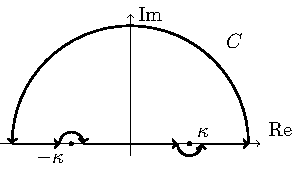
\includegraphics[width = 0.7\columnwidth]{fig/integral-green-tex.pdf}
      \caption{積分経路}\label{Integral}
    \end{figure}
    \par
    次に\refe{formal-soultion}から散乱振幅$f(\theta)$を求める.$V(r')$は$r' < a$でのみ$V\neq 0$であると仮定する.
    \refe{formal-soultion}において
    $r \gg r'$では,
    \begin{align}
      \abs{\bm{r} - \bm{r'}} &= \sqrt{r^2 - 2\bm{r} \cdot \bm{r'} + r'^2} \\
      &= r \qty[1 - \frac{2\bm{r}\cdot\bm{r'}}{r^2} + \qty(\frac{r'}{r})^2]^{1/2} \\
      &\simeq r - \bm{n}\cdot\bm{r'}\label{abs-r-r-prime-approx}
    \end{align}
    が成り立つ.よって,
    \begin{align}
      \e^{\i \kappa \abs{\bm{r} - \bm{r'}}} &\simeq \e^{\i \kappa \qty(r - \bm{n} \cdot \bm{r'})}\\
      &= \e^{\i \kappa r} - \e^{-\i \bm{\kappa} \cdot \bm{r'}}\label{exp-abs-r-r-prime-approx}
    \end{align}
    と近似できる.ただし,$\bm{\kappa'} \coloneqq \kappa \bm{n}$を$z$軸と角度$\theta$をなす散乱方向の波数ベクトルと定義した.
    また,
    \begin{align}
      \frac{1}{\abs{\bm{r} - \bm{r'}}} &= \frac{1}{r}\qty[1 - \frac{2\bm{r}\cdot\bm{r'}}{r^2} + \qty(\frac{r'}{r})^2]^{-1/2} \\ 
      &\simeq \frac{1}{r}\label{abs-r-r-prime-inv-approx}
    \end{align}
    と近似する.% なぜ???
    \refe{exp-abs-r-r-prime-approx}や\refe{abs-r-r-prime-inv-approx}で行った近似結果を\refe{formal-soultion}に代入すると,
    \begin{align}
      \psi(\bm{r}) = \e^{\i kz} - \qty(\frac{1}{4\pi} \int \e^{-\i\bm{\kappa'}\cdot \bm{r'}} \frac{2m}{\hbar^2}V(r')\psi(\bm{r'})\dd{\bm{r'}})\frac{\e^{\i\kappa r}}{r}
    \end{align}
    である.したがって,散乱振幅は
    \begin{align}
      f(\theta) = -\frac{1}{4\pi} \int \dd{\bm{r'}} \e^{- \i \bm{\kappa'} \cdot \bm{r'}} \frac{2m}{\hbar^2}V(r')\psi(\bm{r'})
    \end{align}
    となる.
\end{document}

    \section{Born近似}
      \documentclass{report}
\usepackage{luatexja} % LuaTeXで日本語を使うためのパッケージ
\usepackage{luatexja-fontspec} % LuaTeX用の日本語フォント設定

% --- 数学関連 ---
\usepackage{amsmath, amssymb, amsfonts, mathtools, bm, amsthm} % 基本的な数学パッケージ
\usepackage{type1cm, upgreek} % 数式フォントとギリシャ文字
\usepackage{physics, mhchem} % 物理や化学の記号や式の表記を簡単にする

% --- 表関連 ---
\usepackage{multirow, longtable, tabularx, array, colortbl, dcolumn, diagbox} % 表のレイアウトを柔軟にする
\usepackage{tablefootnote, truthtable} % 表中に注釈を追加、真理値表
\usepackage{tabularray} % 高度な表組みレイアウト

% --- グラフィック関連 ---
\usepackage{tikz, graphicx} % 図の描画と画像の挿入
\usepackage{background} % ウォーターマークの設定
\usepackage{caption, subcaption} % 図や表のキャプション設定
\usepackage{float, here} % 図や表の位置指定

% --- レイアウトとページ設定 ---
\usepackage{fancyhdr} % ページヘッダー、フッター、余白の設定
\usepackage[top = 20truemm, bottom = 20truemm, left = 20truemm, right = 20truemm]{geometry}
\usepackage{fancybox, ascmac} % ボックスのデザイン

% --- 色とスタイル ---
\usepackage{xcolor, color, colortbl, tcolorbox} % 色とカラーボックス
\usepackage{listings, jvlisting} % コードの色付けとフォーマット

% --- 参考文献関連 ---
\usepackage{biblatex, usebib} % 参考文献の管理と挿入
\usepackage{url, hyperref} % URLとリンクの設定

% --- その他の便利なパッケージ ---
\usepackage{footmisc} % 脚注のカスタマイズ
\usepackage{multicol} % 複数段組
\usepackage{comment} % コメントアウトの拡張
\usepackage{siunitx} % 単位の表記
\usepackage{docmute}
% \usepackage{appendix}
% --- tcolorboxとtikzの設定 ---
\tcbuselibrary{theorems, breakable} % 定理のボックスと改ページ設定
\usetikzlibrary{decorations.markings, arrows.meta, calc} % tikzの装飾や矢印の設定

% --- 定理スタイルと数式設定 ---
\theoremstyle{definition} % 定義スタイル
\numberwithin{equation}{section} % 式番号をサブセクション単位でリセット

% --- hyperrefの設定 ---
\hypersetup{
  setpagesize = false,
  bookmarks = true,
  bookmarksdepth = tocdepth,
  bookmarksnumbered = true,
  colorlinks = false,
  pdftitle = {}, % PDFタイトル
  pdfsubject = {}, % PDFサブジェクト
  pdfauthor = {}, % PDF作者
  pdfkeywords = {} % PDFキーワード
}

% --- siunitxの設定 ---
\sisetup{
  table-format = 1.5, % 小数点以下の桁数
  table-number-alignment = center, % 数値の中央揃え
}

% --- 透かし画像の設定 --- 
\backgroundsetup{
  scale=0.5,                       % 画像のスケール
  % color=black,                   % 画像の色(透かし用に半透明が推奨)
  opacity=0.2,                   % 透かしの透明度(0が完全透明、1が完全不透明)
  angle=0,                       % 画像の角度
  position = current page.south east,  % ページの右下
  hshift=-6cm, % 右方向へのシフト(負の値で内側に移動)
  vshift=5cm,  % 上方向へのシフト(正の値で内側に移動)
  contents={
\includegraphics{./fig/appilogo-circular-full.png}} % 画像のパス
}

% --- その他の設定 ---
\allowdisplaybreaks % 数式の途中改ページ許可
\newcolumntype{t}{!{\vrule width 0.1pt}} % 新しいカラムタイプ
\newcolumntype{b}{!{\vrule width 1.5pt}} % 太いカラム
\UseTblrLibrary{amsmath, booktabs, counter, diagbox, functional, hook, html, nameref, siunitx, varwidth, zref} % tabularrayのライブラリ
\setlength{\columnseprule}{0.4pt} % カラム区切り線の太さ
\captionsetup[figure]{font = bf} % 図のキャプションの太字設定
\captionsetup[table]{font = bf} % 表のキャプションの太字設定
\captionsetup[lstlisting]{font = bf} % コードのキャプションの太字設定
\captionsetup[subfigure]{font = bf, labelformat = simple} % サブ図のキャプション設定
\setcounter{secnumdepth}{4} % セクションの深さ設定
\newcolumntype{d}{D{.}{.}{5}} % 数値のカラム
\newcolumntype{M}[1]{>{\centering\arraybackslash}m{#1}} % センター揃えのカラム
\DeclareMathOperator{\diag}{diag}
\everymath{\displaystyle} % 数式のスタイル
\newcommand{\inner}[2]{\left\langle #1, #2 \right\rangle}
\renewcommand{\figurename}{図}
\renewcommand{\i}{\mathrm{i}} % 複素数単位i
\renewcommand{\laplacian}{\grad^2} % ラプラシアンの記号
\renewcommand{\thesubfigure}{(\alph{subfigure})} % サブ図の番号形式
\newcommand{\m}[3]{\multicolumn{#1}{#2}{#3}} % マルチカラムのショートカット
\renewcommand{\r}[1]{\mathrm{#1}} % mathrmのショートカット
\newcommand{\e}{\mathrm{e}} % 自然対数の底e
\newcommand{\Ef}{E_{\mathrm{F}}} % フェルミエネルギー
\renewcommand{\c}{\si{\degreeCelsius}} % 摂氏記号
\renewcommand{\d}{\r{d}} % d記号
\renewcommand{\t}[1]{\texttt{#1}} % タイプライタフォント
\newcommand{\kb}{k_{\mathrm{B}}} % ボルツマン定数
% \renewcommand{\phi}{\varphi} % ϕをφに変更
\renewcommand{\epsilon}{\varepsilon}
\newcommand{\fullref}[1]{\textbf{\ref{#1} \nameref{#1}}}
\newcommand{\reff}[1]{\textbf{図\ref{#1}}} % 図参照のショートカット
\newcommand{\reft}[1]{\textbf{表\ref{#1}}} % 表参照のショートカット
\newcommand{\refe}[1]{\textbf{式\eqref{#1}}} % 式参照のショートカット
\newcommand{\refp}[1]{\textbf{コード\ref{#1}}} % コード参照のショートカット
\renewcommand{\lstlistingname}{コード} % コードリストの名前
\renewcommand{\theequation}{\thesection.\arabic{equation}} % 式番号の形式
\renewcommand{\footrulewidth}{0.4pt} % フッターの線
\newcommand{\mar}[1]{\textcircled{\scriptsize #1}} % 丸囲み文字
\newcommand{\combination}[2]{{}_{#1} \mathrm{C}_{#2}} % 組み合わせ
\newcommand{\thline}{\noalign{\hrule height 0.1pt}} % 細い横線
\newcommand{\bhline}{\noalign{\hrule height 1.5pt}} % 太い横線

% --- カスタム色定義 ---
\definecolor{burgundy}{rgb}{0.5, 0.0, 0.13} % バーガンディ色
\definecolor{charcoal}{rgb}{0.21, 0.27, 0.31} % チャコール色
\definecolor{forest}{rgb}{0.0, 0.35, 0} % 森の緑色

% --- カスタム定理環境の定義 ---
\newtcbtheorem[number within = chapter]{myexc}{練習問題}{
  fonttitle = \gtfamily\sffamily\bfseries\upshape,
  colframe = forest,
  colback = forest!2!white,
  rightrule = 1pt,
  leftrule = 1pt,
  bottomrule = 2pt,
  colbacktitle = forest,
  theorem style = standard,
  breakable,
  arc = 0pt,
}{exc-ref}
\newtcbtheorem[number within = chapter]{myprop}{命題}{
  fonttitle = \gtfamily\sffamily\bfseries\upshape,
  colframe = blue!50!black,
  colback = blue!50!black!2!white,
  rightrule = 1pt,
  leftrule = 1pt,
  bottomrule = 2pt,
  colbacktitle = blue!50!black,
  theorem style = standard,
  breakable,
  arc = 0pt
}{proposition-ref}
\newtcbtheorem[number within = chapter]{myrem}{注意}{
  fonttitle = \gtfamily\sffamily\bfseries\upshape,
  colframe = yellow!20!black,
  colback = yellow!50,
  rightrule = 1pt,
  leftrule = 1pt,
  bottomrule = 2pt,
  colbacktitle = yellow!20!black,
  theorem style = standard,
  breakable,
  arc = 0pt
}{remark-ref}
\newtcbtheorem[number within = chapter]{myex}{例題}{
  fonttitle = \gtfamily\sffamily\bfseries\upshape,
  colframe = black,
  colback = white,
  rightrule = 1pt,
  leftrule = 1pt,
  bottomrule = 2pt,
  colbacktitle = black,
  theorem style = standard,
  breakable,
  arc = 0pt
}{example-ref}
\newtcbtheorem[number within = chapter]{exc}{Requirement}{myexc}{exc-ref}
\newcommand{\rqref}[1]{{\bfseries\sffamily 練習問題 \ref{exc-ref:#1}}}
\newtcbtheorem[number within = chapter]{definition}{Definition}{mydef}{definition-ref}
\newcommand{\dfref}[1]{{\bfseries\sffamily 定義 \ref{definition-ref:#1}}}
\newtcbtheorem[number within = chapter]{prop}{命題}{myprop}{proposition-ref}
\newcommand{\prref}[1]{{\bfseries\sffamily 命題 \ref{proposition-ref:#1}}}
\newtcbtheorem[number within = chapter]{rem}{注意}{myrem}{remark-ref}
\newcommand{\rmref}[1]{{\bfseries\sffamily 注意 \ref{remark-ref:#1}}}
\newtcbtheorem[number within = chapter]{ex}{例題}{myex}{example-ref}
\newcommand{\exref}[1]{{\bfseries\sffamily 例題 \ref{example-ref:#1}}}
% --- 再定義コマンド ---
% \mathtoolsset{showonlyrefs=true} % 必要な式番号のみ表示
\pagestyle{fancy} % ヘッダー・フッターのスタイル設定
\chead{応用量子物性講義ノート} % 中央ヘッダー
% \rhead{}
\fancyhead[R]{\rightmark}
\renewcommand{\sectionmark}[1]{\markright{\thesection\ #1}}
\cfoot{\thepage} % 中央フッターにページ番号
\lhead{}
\rfoot{Yuto Masuda and Haruki Aoki} % 右フッターに名前
\setcounter{tocdepth}{4} % 目次の深さ
\makeatletter
\@addtoreset{equation}{section} % サブセクションごとに式番号をリセット
\makeatother

% --- メタ情報 ---
\title{応用量子物性講義ノート}
\date{更新日\today}
\author{Yuto Masuda and Haruki Aoki}

\begin{document}
  一般に,散乱の波動関数は,
  \begin{align}
    \psi(\bm{r}) = \e^{\i kz} + \int G_0 (\bm{r} - \bm{r'}) \frac{2m}{\hbar^2} V(r') \psi(\bm{r'}) \dd{\bm{r'}}\label{wave-funtion-of-scattering}
  \end{align}
  と表されるのであった.
  この波動関数を厳密に求めることは困難であるため近似を考える.
  まず,\refe{wave-funtion-of-scattering}を簡略化して,
  \begin{align}
    \psi(\bm{r}) = \psi_0 + \int g V \psi(\bm{r}') \dd{\bm{r}'}\label{simple-wave-funtion-of-scattering}
  \end{align}
  と表現する.
  ただし,
  \begin{align}
    g(\bm{r}) \coloneqq G_0(\bm{r})\frac{2m}{\hbar^2}
  \end{align}
  である.
  \refe{simple-wave-funtion-of-scattering}を再帰的に代入すると,
  \begin{align}
    \psi(\bm{r}) &= \psi_0 + \int g V \psi(\bm{r'}) \dd{\bm{r'}} \\
    &= \psi_0 + \int gV \qty(\psi_0 + \int g V \psi(\bm{r''}) \dd{\bm{r''}}) \dd{\bm{r'}} \\
    &= \psi_0 + \int g V \psi_0(\bm{r'}) \dd{\bm{r'}} + \iint gVgV \psi(\bm{r''}) \dd{\bm{r'}} \dd{\bm{r''}} \\
    &= \psi_0 + \int g V \psi_0(\bm{r'}) \dd{\bm{r'}} + \iint gVgV \psi_0(\bm{r''}) \dd{\bm{r'}} \dd{\bm{r''}} + \iiint gVgVgV \psi_0(\bm{r'''}) \dd{\bm{r'}} \dd{\bm{r''}} \dd{\bm{r'''}} + \cdots\label{dozens-of-gv}
  \end{align}
  を得る.
  \refe{dozens-of-gv}を第1項までで近似して,残りの項を捨てる.
  これは散乱の波動関数を平面波で近似することに相当する.
  つまり,
  \begin{align}
    \psi \simeq \psi_0
  \end{align}
  とする.これを\textbf{第1 Born近似}という\footnote{Max Born(1882-1970)}\footnote{砂川,散乱の量子論,
  「第1 Born近似がとくによく利用される理由は,何といってもその簡単さにある.したがって,ある散乱問題を手がけたとき,だれもが最初に試してみるのが,この近似である.
  そして思わしい結果がえられないとき,他の近似法を考えるのである.」}.
  \par
  Born近似を用いて散乱振幅を求める.$\bm{k} \coloneqq k\bm{e}_z$,$\bm{r} \coloneqq z\bm{e}_z$とすると,
  $\psi(\bm{r}') = \e^{\i kz} = \e^{\i \bm{k}\cdot\bm{r}'}$となるから,
  \begin{align}
    f^{(1)}(\theta) &= -\frac{1}{4\pi} \int \e^{\i \bm{\kappa'}\cdot\bm{r'}} \frac{2m}{\hbar} V(r') \psi(\bm{r'}) \dd{\bm{r'}} \\
    &= -\frac{1}{4\pi}\frac{2m}{\hbar^2}\int\e^{-\i (\bm{\kappa'} - \bm{k})\cdot\bm{r}'} V(r') \dd{\bm{r}'} \\
    &= -\frac{1}{4\pi}\frac{2m}{\hbar^2}\int\e^{-\i \bm{q}\cdot \bm{r}'} V(r') \dd{\bm{r}'}\label{potential-fourier-transform}
  \end{align}
  となる.ただし,散乱による運動量変化に対応する物理量を$\bm{q} \coloneqq \bm{\kappa'} - \bm{k}$と定義した.
  \refe{potential-fourier-transform}を見ると,散乱振幅はポテンシャル$V(r)$のFourier変換から得られることがわかる\footnote{
    $f^{(n)}$は第$n$ Born近似による散乱振幅を意味する.
  }.
  また,球対称ポテンシャルのとき\refe{potential-fourier-transform}は簡略化できて,
  \begin{align}
    f^{(1)}(\theta) &= -\frac{1}{4\pi}\frac{2m}{\hbar^2}\int\e^{-\i \bm{q}\cdot \bm{r}'} V(r') \dd{\bm{r}'}\\
    &= -\frac{1}{4\pi}\frac{2m}{\hbar^2} \int_{\phi' = 0}^{2\pi}\dd{\phi'} \int_{\theta' = 0}^{\pi}\dd{\theta'}\int_{r' = 0}^{\infty}r'^2 \sin\theta' \dd{r'} \e^{-\i qr' \cos\theta'} V(r') \\
    &= -\frac{1}{4\pi}\frac{2m}{\hbar^2} 2\pi \int_{r' = 0}^{\infty}V(r')r'^2\int_{\theta' = 0}^{\pi} \e^{-\i qr' \cos\theta'} \sin\theta' \dd{r'}\dd{\theta'} \\ 
    &= -\frac{m}{\hbar^2} \int_{0}^{\infty} r'^2V(r') \frac{\e^{\i qr'} - \e^{-\i qr'}}{\i qr'} \dd{r'} \\ 
    &= -\frac{m}{\hbar^2} \int_{0}^{\infty} rV(r) \frac{\e^{\i qr} - \e^{-\i qr}}{\i q} \dd{r} \\ 
    &= -\frac{2m}{\hbar^2 q} \int_{0}^{\infty} rV(r)\sin\qty(qr) \dd{r}
  \end{align}
  となる.
  \begin{itembox}[l]{球対称ポテンシャルの散乱振幅}
    \begin{align}
      f^{(1)}(\theta) &= -\frac{m}{\hbar^2} \int_{0}^{\infty} rV(r) \frac{\e^{\i qr} - \e^{-\i qr}}{\i q} \dd{r}\label{SCamp1st-exp} \\ 
      &= -\frac{2m}{\hbar^2 q} \int_{0}^{\infty} rV(r)\sin\qty(qr) \dd{r}\label{SCamp1st-sin}
    \end{align}
  \end{itembox}
  \begin{myex}{湯川ポテンシャル}{}
    球対称ポテンシャル$V(r)$が,湯川ポテンシャルの場合を考える.
    湯川ポテンシャルは,
    \begin{align}
      V(r) = V_0 \frac{\e^{-\mu r}}{\mu r}
    \end{align}
    と書ける.
    による散乱を考える\footnote{湯川秀樹(1907-1981)}.これは,$V(r)$の到達距離が$\mu^{-1}$ほどであり,核子同士に働く力を表す.
    物質中では,伝導電子に遮蔽された不純物のCoulombポテンシャルを表す.
    $\mu = 1,2$及びCoulombポテンシャルのグラフを\reff{yukawa-potential-graph}に示す.
    このポテンシャルの下で散乱振幅$f^{(1)}(\theta)$と散乱断面積$\sigma^{(1)}(\theta)$を求めよ.
    \tcblower
    散乱振幅は\refe{SCamp1st-exp}より,
    \begin{align}
      f^{(1)}(\theta) &= -\frac{m}{\hbar^2} \int_{0}^{\infty} rV(r) \frac{\e^{\i qr} - \e^{-\i qr}}{\i q} \dd{r} \\ 
      &= -\frac{m}{\i \hbar^2 q \mu} \int_{0}^{\infty} rV_0\frac{e^{-\mu r}}{\mu r} \frac{\e^{\i qr} - \e^{-\i qr}}{\i q}\dd{r} \\
      &= -\frac{mV_0}{\i \hbar^2 q \mu} \int_{0}^{\infty} \qty[\exp\qty{(-\mu + \i q)r} - \exp\qty{(-\mu - \i q)r}] \dd{r} \\
      &= - \frac{2m V_0}{\hbar^2 \mu} \frac{1}{\mu^2 + q^2}
    \end{align}
    \par
    散乱振幅は,
    \begin{align}
      \sigma^{(1)}(\theta) &= \abs{f^{(1)}(\theta)}^2\\
      &= \qty(\frac{2m V_0}{\hbar^2 \mu})^2 \frac{1}{(\mu^2 + q^2)^2}\\
      &= \qty(\frac{2m V_0}{\hbar^2 \mu})^2 \frac{1}{\qty[\mu^2 + 4k^2 \sin^2\qty(\theta/2)]^2}
    \end{align}
    である.なお,$\bm{\kappa'}$と$\bm{k}$のなす角が$\theta$であるので余弦定理より,$q = 2k\sin\theta/2$であることを用いた.
    \begin{figure}[H]
      \centering
      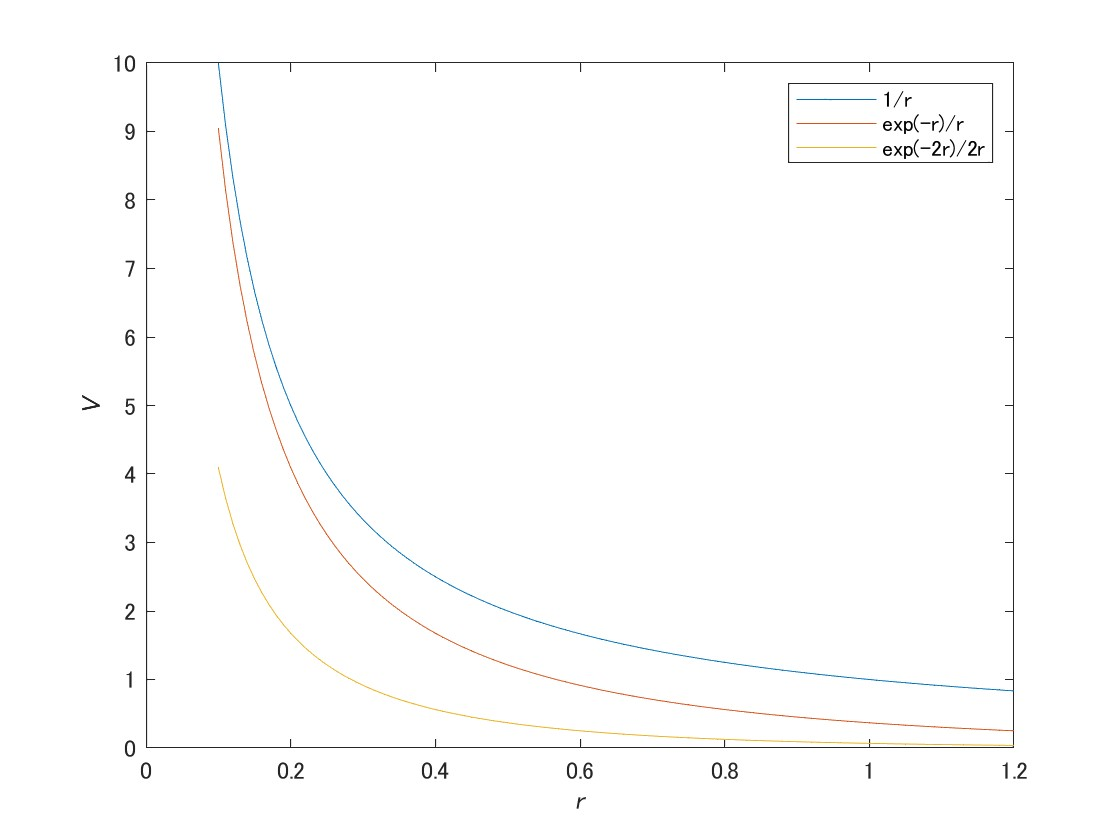
\includegraphics[width = 0.8\columnwidth]{fig/yukawa_potential.jpg}
      \caption{湯川ポテンシャルとCoulombポテンシャルの比較}\label{yukawa-potential-graph}
    \end{figure}
  \end{myex}
  \begin{myex}{Rutherford散乱(Griffith Example 10.6)}{}
    湯川ポテンシャルで$V_0 = \frac{q_1q_2}{4\pi \epsilon_0}$,$\mu = 0$とするとCoulombポテンシャル
    \begin{align}
      V(r) = \frac{q_1q_2}{4\pi\epsilon_0}
    \end{align}
    と一致する.式(\ref{SCamp1st-sin})に代入して散乱振幅を求める.
    \begin{align}
      f(\theta) &= - \frac{2m}{\hbar^2q} \int_{0}^{\infty} r \frac{q_1q_2}{4\pi\epsilon_0 r} \sin\qty(qr) \dd{r}\\
      &= -\frac{2m}{\hbar^2q}\frac{q_1q_2}{4\pi\epsilon_0}\int_{0}^{\infty} \sin\qty(qr) \dd{r} \\
      &=  -\frac{2m}{\hbar^2q}\frac{q_1q_2}{4\pi\epsilon_0}\qty(-\frac{1}{q}\qty[\cos\qty(qr)]_0^{\infty})\\
      &\simeq - \frac{mq_1q_1}{2\pi\epsilon_0\hbar^2q^2}\\
      &= - \frac{mq_1q_1}{8\pi\epsilon_0\hbar^2 \sin^2 \theta/2}
    \end{align}
  \end{myex}
\end{document}
    \section{部分波展開}
      \documentclass{report}
\usepackage{luatexja} % LuaTeXで日本語を使うためのパッケージ
\usepackage{luatexja-fontspec} % LuaTeX用の日本語フォント設定

% --- 数学関連 ---
\usepackage{amsmath, amssymb, amsfonts, mathtools, bm, amsthm} % 基本的な数学パッケージ
\usepackage{type1cm, upgreek} % 数式フォントとギリシャ文字
\usepackage{physics, mhchem} % 物理や化学の記号や式の表記を簡単にする

% --- 表関連 ---
\usepackage{multirow, longtable, tabularx, array, colortbl, dcolumn, diagbox} % 表のレイアウトを柔軟にする
\usepackage{tablefootnote, truthtable} % 表中に注釈を追加、真理値表
\usepackage{tabularray} % 高度な表組みレイアウト

% --- グラフィック関連 ---
\usepackage{tikz, graphicx} % 図の描画と画像の挿入
\usepackage{background} % ウォーターマークの設定
\usepackage{caption, subcaption} % 図や表のキャプション設定
\usepackage{float, here} % 図や表の位置指定

% --- レイアウトとページ設定 ---
\usepackage{fancyhdr} % ページヘッダー、フッター、余白の設定
\usepackage[top = 20truemm, bottom = 20truemm, left = 20truemm, right = 20truemm]{geometry}
\usepackage{fancybox, ascmac} % ボックスのデザイン

% --- 色とスタイル ---
\usepackage{xcolor, color, colortbl, tcolorbox} % 色とカラーボックス
\usepackage{listings, jvlisting} % コードの色付けとフォーマット

% --- 参考文献関連 ---
\usepackage{biblatex, usebib} % 参考文献の管理と挿入
\usepackage{url, hyperref} % URLとリンクの設定

% --- その他の便利なパッケージ ---
\usepackage{footmisc} % 脚注のカスタマイズ
\usepackage{multicol} % 複数段組
\usepackage{comment} % コメントアウトの拡張
\usepackage{siunitx} % 単位の表記
\usepackage{docmute}
% \usepackage{appendix}
% --- tcolorboxとtikzの設定 ---
\tcbuselibrary{theorems, breakable} % 定理のボックスと改ページ設定
\usetikzlibrary{decorations.markings, arrows.meta, calc} % tikzの装飾や矢印の設定

% --- 定理スタイルと数式設定 ---
\theoremstyle{definition} % 定義スタイル
\numberwithin{equation}{section} % 式番号をサブセクション単位でリセット

% --- hyperrefの設定 ---
\hypersetup{
  setpagesize = false,
  bookmarks = true,
  bookmarksdepth = tocdepth,
  bookmarksnumbered = true,
  colorlinks = false,
  pdftitle = {}, % PDFタイトル
  pdfsubject = {}, % PDFサブジェクト
  pdfauthor = {}, % PDF作者
  pdfkeywords = {} % PDFキーワード
}

% --- siunitxの設定 ---
\sisetup{
  table-format = 1.5, % 小数点以下の桁数
  table-number-alignment = center, % 数値の中央揃え
}

% --- 透かし画像の設定 --- 
\backgroundsetup{
  scale=0.5,                       % 画像のスケール
  % color=black,                   % 画像の色(透かし用に半透明が推奨)
  opacity=0.2,                   % 透かしの透明度(0が完全透明、1が完全不透明)
  angle=0,                       % 画像の角度
  position = current page.south east,  % ページの右下
  hshift=-6cm, % 右方向へのシフト(負の値で内側に移動)
  vshift=5cm,  % 上方向へのシフト(正の値で内側に移動)
  contents={
\includegraphics{./fig/appilogo-circular-full.png}} % 画像のパス
}

% --- その他の設定 ---
\allowdisplaybreaks % 数式の途中改ページ許可
\newcolumntype{t}{!{\vrule width 0.1pt}} % 新しいカラムタイプ
\newcolumntype{b}{!{\vrule width 1.5pt}} % 太いカラム
\UseTblrLibrary{amsmath, booktabs, counter, diagbox, functional, hook, html, nameref, siunitx, varwidth, zref} % tabularrayのライブラリ
\setlength{\columnseprule}{0.4pt} % カラム区切り線の太さ
\captionsetup[figure]{font = bf} % 図のキャプションの太字設定
\captionsetup[table]{font = bf} % 表のキャプションの太字設定
\captionsetup[lstlisting]{font = bf} % コードのキャプションの太字設定
\captionsetup[subfigure]{font = bf, labelformat = simple} % サブ図のキャプション設定
\setcounter{secnumdepth}{4} % セクションの深さ設定
\newcolumntype{d}{D{.}{.}{5}} % 数値のカラム
\newcolumntype{M}[1]{>{\centering\arraybackslash}m{#1}} % センター揃えのカラム
\DeclareMathOperator{\diag}{diag}
\everymath{\displaystyle} % 数式のスタイル
\newcommand{\inner}[2]{\left\langle #1, #2 \right\rangle}
\renewcommand{\figurename}{図}
\renewcommand{\i}{\mathrm{i}} % 複素数単位i
\renewcommand{\laplacian}{\grad^2} % ラプラシアンの記号
\renewcommand{\thesubfigure}{(\alph{subfigure})} % サブ図の番号形式
\newcommand{\m}[3]{\multicolumn{#1}{#2}{#3}} % マルチカラムのショートカット
\renewcommand{\r}[1]{\mathrm{#1}} % mathrmのショートカット
\newcommand{\e}{\mathrm{e}} % 自然対数の底e
\newcommand{\Ef}{E_{\mathrm{F}}} % フェルミエネルギー
\renewcommand{\c}{\si{\degreeCelsius}} % 摂氏記号
\renewcommand{\d}{\r{d}} % d記号
\renewcommand{\t}[1]{\texttt{#1}} % タイプライタフォント
\newcommand{\kb}{k_{\mathrm{B}}} % ボルツマン定数
% \renewcommand{\phi}{\varphi} % ϕをφに変更
\renewcommand{\epsilon}{\varepsilon}
\newcommand{\fullref}[1]{\textbf{\ref{#1} \nameref{#1}}}
\newcommand{\reff}[1]{\textbf{図\ref{#1}}} % 図参照のショートカット
\newcommand{\reft}[1]{\textbf{表\ref{#1}}} % 表参照のショートカット
\newcommand{\refe}[1]{\textbf{式\eqref{#1}}} % 式参照のショートカット
\newcommand{\refp}[1]{\textbf{コード\ref{#1}}} % コード参照のショートカット
\renewcommand{\lstlistingname}{コード} % コードリストの名前
\renewcommand{\theequation}{\thesection.\arabic{equation}} % 式番号の形式
\renewcommand{\footrulewidth}{0.4pt} % フッターの線
\newcommand{\mar}[1]{\textcircled{\scriptsize #1}} % 丸囲み文字
\newcommand{\combination}[2]{{}_{#1} \mathrm{C}_{#2}} % 組み合わせ
\newcommand{\thline}{\noalign{\hrule height 0.1pt}} % 細い横線
\newcommand{\bhline}{\noalign{\hrule height 1.5pt}} % 太い横線

% --- カスタム色定義 ---
\definecolor{burgundy}{rgb}{0.5, 0.0, 0.13} % バーガンディ色
\definecolor{charcoal}{rgb}{0.21, 0.27, 0.31} % チャコール色
\definecolor{forest}{rgb}{0.0, 0.35, 0} % 森の緑色

% --- カスタム定理環境の定義 ---
\newtcbtheorem[number within = chapter]{myexc}{練習問題}{
  fonttitle = \gtfamily\sffamily\bfseries\upshape,
  colframe = forest,
  colback = forest!2!white,
  rightrule = 1pt,
  leftrule = 1pt,
  bottomrule = 2pt,
  colbacktitle = forest,
  theorem style = standard,
  breakable,
  arc = 0pt,
}{exc-ref}
\newtcbtheorem[number within = chapter]{myprop}{命題}{
  fonttitle = \gtfamily\sffamily\bfseries\upshape,
  colframe = blue!50!black,
  colback = blue!50!black!2!white,
  rightrule = 1pt,
  leftrule = 1pt,
  bottomrule = 2pt,
  colbacktitle = blue!50!black,
  theorem style = standard,
  breakable,
  arc = 0pt
}{proposition-ref}
\newtcbtheorem[number within = chapter]{myrem}{注意}{
  fonttitle = \gtfamily\sffamily\bfseries\upshape,
  colframe = yellow!20!black,
  colback = yellow!50,
  rightrule = 1pt,
  leftrule = 1pt,
  bottomrule = 2pt,
  colbacktitle = yellow!20!black,
  theorem style = standard,
  breakable,
  arc = 0pt
}{remark-ref}
\newtcbtheorem[number within = chapter]{myex}{例題}{
  fonttitle = \gtfamily\sffamily\bfseries\upshape,
  colframe = black,
  colback = white,
  rightrule = 1pt,
  leftrule = 1pt,
  bottomrule = 2pt,
  colbacktitle = black,
  theorem style = standard,
  breakable,
  arc = 0pt
}{example-ref}
\newtcbtheorem[number within = chapter]{exc}{Requirement}{myexc}{exc-ref}
\newcommand{\rqref}[1]{{\bfseries\sffamily 練習問題 \ref{exc-ref:#1}}}
\newtcbtheorem[number within = chapter]{definition}{Definition}{mydef}{definition-ref}
\newcommand{\dfref}[1]{{\bfseries\sffamily 定義 \ref{definition-ref:#1}}}
\newtcbtheorem[number within = chapter]{prop}{命題}{myprop}{proposition-ref}
\newcommand{\prref}[1]{{\bfseries\sffamily 命題 \ref{proposition-ref:#1}}}
\newtcbtheorem[number within = chapter]{rem}{注意}{myrem}{remark-ref}
\newcommand{\rmref}[1]{{\bfseries\sffamily 注意 \ref{remark-ref:#1}}}
\newtcbtheorem[number within = chapter]{ex}{例題}{myex}{example-ref}
\newcommand{\exref}[1]{{\bfseries\sffamily 例題 \ref{example-ref:#1}}}
% --- 再定義コマンド ---
% \mathtoolsset{showonlyrefs=true} % 必要な式番号のみ表示
\pagestyle{fancy} % ヘッダー・フッターのスタイル設定
\chead{応用量子物性講義ノート} % 中央ヘッダー
% \rhead{}
\fancyhead[R]{\rightmark}
\renewcommand{\sectionmark}[1]{\markright{\thesection\ #1}}
\cfoot{\thepage} % 中央フッターにページ番号
\lhead{}
\rfoot{Yuto Masuda and Haruki Aoki} % 右フッターに名前
\setcounter{tocdepth}{4} % 目次の深さ
\makeatletter
\@addtoreset{equation}{section} % サブセクションごとに式番号をリセット
\makeatother

% --- メタ情報 ---
\title{応用量子物性講義ノート}
\date{更新日\today}
\author{Yuto Masuda and Haruki Aoki}

\begin{document}
  近似法の一つである部分波展開を扱う.
  まず,半古典論を用いて散乱が起こる条件から,方位量子数$l$ごとに波動関数を展開して,$l$が小さい波動関数のみ考えればよいことが分かる.
  次に,波動関数の基底展開について議論を行う.関数空間には様々な直交基底が存在するが,今回はLegendre多項式を基底に取る.
  最後に,展開に用いた未定係数を用いて,散乱断面積や全断面積をその未定係数を用いて表す.
  \subsection{散乱の条件}
    古典力学において角運動量$\bm{L}$は,
    \begin{align}
      \bm{L} = \bm{r} \times \bm{p} = m\bm{r} \times \bm{v}
    \end{align}
    と書けるのであった.
    球対称ポテンシャルの下では,
    \begin{align}
      \dv{\bm{L}}{t} &= m\dv{\bm{r}}{t} \times \bm{v} + m\bm{r} \times \dv{\bm{v}}{t} \\
      &= \bm{r} \times \bm{F} \\
      &= \bm{r} \times (-\grad V(r)) \\
      &= \bm{r} \times \abs{\grad V}\frac{\bm{r}}{r} \\
      &= 0
    \end{align}
    より,角運動量は保存される.
    衝突パラメータを$b$,運動量を$\bm{p}$とした粒子の角運動量は,
    \begin{align}
      \abs{\bm{L}} &= \abs{\bm{r} \times \bm{p}} \\
      &= pb
    \end{align}
    である.散乱体を半径$a$の球とすると,衝突の条件は
    \begin{align}
      b &< a \\
      L/p &< a \\
      L &< pa \label{ConditionofSC}
    \end{align}
    である.つまり,角運動量が小さい粒子のみ散乱することがわかる.
    \par
    \refe{ConditionofSC}を半古典的な散乱条件へ書き直すことを考える.
    量子力学では,角運動量の大きさ$L$は,$l = 0, 1, 2, \cdots$の値を取る方位量子数$l$を用いて$L = \hbar \sqrt{l(l + 1)}$と書けるので,
    衝突の条件は,
    \begin{align}
      L = \hbar \sqrt{l(l + 1)} < pa = \hbar ka\label{scattering-condition-of-l}
    \end{align}
    と書ける.\refe{scattering-condition-of-l}を見れば,散乱の影響を受けるのは$l$が小さいときのみであることがわかる.
    よって波動関数を,
    \begin{align}
      \psi = \phi^{(l = 0)} + \phi^{(l = 1)} + \cdots
    \end{align}
    のように異なる$l$に属する固有関数で展開し,$l$が小さい状態についてだけ散乱の影響を考える.これを\textbf{部分波展開}という.
  \subsection{波動関数の基底展開}
    さて,\refe{psi-r-in-sc-k}で示した散乱の波動関数,
    \begin{align}
      \psi(\bm{r}) = \e^{\i kz} + f(\theta)\frac{\e^{\i kr}}{r}
    \end{align}
    を部分波展開する\footnote{ここから\refe{PartialWave}までは飛ばしても良い.}ことを考える.
    まず,Legendre多項式の性質を調べて,直交性を知る.
    次に,Legendre多項式を用いて波動関数を展開して,展開係数$B_{ml}$が満たすべき微分方程式を導く.
    続いて,Besselの微分方程式の解であるBessel関数の表式を求めて,球Bessel関数と球Neumann関数,球Hankel関数を定義する.
    最後に,展開係数$B_{ml}$が球Bessel関数と球Neumann関数の線型結合で書けることを確かめて,線型結合の係数が波動関数を特徴づけるものだと知る.
    \subsubsection{Strum-Liouvillle演算子のHermite性}
      $a < b$として,$x\in \qty[a, b]$で定義された関数空間$V$を考える.$\rho(x)$を非負の実数関数として,$f, g\in V$に対して,
      \begin{align}
        \inner{f}{g} \coloneqq \int_{a}^{b} f^*(x)g(x)\rho(x)\dd{x}
      \end{align}
      なる内積を入れる.
      関数空間$V$上の演算子として$\mathcal{L}$を,
      \begin{align}
        \mathcal{L} \coloneqq \frac{1}{\rho(x)}\qty[\dv{x}\qty{p(x)\dv{x}} + q(x)]\label{strum-liouville-operator-def}
      \end{align}
      とする.
      \refe{strum-liouville-operator-def}なる形をした演算子をStrum-Liouvillle演算子という.
      境界条件を,$\forall f \in V$について,
      \begin{align}
        \begin{dcases}
          f(a) = f(b) \\ 
          p(a)f'(a) = p(b)f'(b)
        \end{dcases}
      \end{align}
      とすると,
      \begin{align}
        \inner{f}{\mathcal{L}g} = \inner{\mathcal{L}f}{g}\label{hermite-def}
      \end{align}
      が成立する.
      \refe{hermite-def}なる関係が成り立つ演算子$\mathcal{L}$をHermite演算子という.
      \begin{proof}
        内積の定義より,
        \begin{align}
          \inner{f}{\mathcal{L}g} &= \int_{a}^{b} f^*(x)\frac{1}{\rho(x)}\qty[\dv{x}\qty{p(x)\dv{x}g(x)} + q(x)g(x)]\rho(x)\dd{x} \\ 
          &= \int_{a}^{b} f^*(x)\qty[\dv{x}\qty{p(x)\dv{x}g(x)} + q(x)g(x)]\dd{x} \\ 
          &= \qty[f^*(x)g'(x)]_{a}^{b} - \int_{a}^{b}f'^*(x)p(x)g'(x)\dd{x} + \int_{a}^{b}f^*(x)q(x)g(x)\dd{x} \\ 
          &= \qty[f^*(x)p(x)g'(x)]_{a}^{b} - \qty[f'^*(x)p(x)g(x)]_{a}^{b} + \int_{a}^{b}g(x)\frac{1}{\rho(x)}\qty[\dv{x}\qty(p(x)\dv{x}f^*(x)) + q(x)f^*(x)]\rho(x)\dd{x} \\ 
          &= \qty[f^*(x)p(x)g'(x)]_{a}^{b} - \qty[f'^*(x)p(x)g(x)]_{a}^{b} + \inner{g}{\mathcal{L}f}^* \\ 
          &= \qty[f^*(x)p(x)g'(x)]_{a}^{b} - \qty[g(x)p(x)f'^*(x)]_{a}^{b} + \inner{\mathcal{L}f}{g} 
        \end{align}
        となる.第1項と第2項について,第1項に$f(a) = f(b)$を,第2項に$p(x)$が実数値関数であり$p(a)f'(a) = p(b)f'(b)$であることを用いると
        \begin{align}
          \qty[f^*(x)p(x)g'(x)]_{a}^{b} - \qty[f'^*(x)p(x)g(x)]_{a}^{b} = \qty{p(b)g'(b) - p(a)f(a)}f^*(a) - \qty{g(b) - g(a)}p(a)f'(a)
        \end{align}
        を得る.今度は,第1項に$p(x)$が実数値関数であり$p(a)g'(a) = p(b)g'(b)$であることを,第2項に$g(a) = g(b)$を用いれば,
        \begin{align}
          \inner{f}{\mathcal{L}g} = \inner{\mathcal{L}f}{g}
        \end{align}
        を得る.
      \end{proof}
    \subsubsection{Legendre多項式}
      \refe{strum-liouville-operator-def}において,$a = -b = 1$とする.また,
      \begin{align}
        \rho(x) &\coloneqq 1 \\ 
        p(x) &\coloneqq 1 - x^2 \\ 
        q(x) &\coloneqq -\frac{m^2}{1 - x^2},\ m\in \qty{0, 1, \cdots}
      \end{align}
      とすると,
      \begin{align}
        \mathcal{L}_m = \dv{x}\qty{(1 - x^2)\dv{x}} - \frac{m^2}{1 - x^2}
      \end{align}
      となる.
      関数の内積は,
      \begin{align}
        \inner{f}{g} = \int_{-1}^{1} f^*(x)g(x) \dd{x} \label{inner-prod-legendre}
      \end{align}
      と定義しておく.
      また,境界条件は,
      \begin{align}
        p(\pm 1)f^*(\pm 1)g'(\pm 1) = 0
      \end{align}
      とする.これより,演算子$\mathcal{L}$がHermite演算子であると確かめられる.
      たとえば,$g'(x) = p(x)$となるように$g(x)$を定めれば,$f(1) = f(-1) = 0$となる.
      また,$f(x) = 1$となるように$f(x)$を定めれば,$p(1)g'(1) = p(-1)g'(1) = 0$となるので,前節で示した境界条件を満足する.
      さて,Legendre多項式$P_n(x)$は$n$を非負整数として,
      \begin{align}
        \mathcal{L}_0P_n(x) &= -n(n + 1) P_n(x) \\ 
        \Leftrightarrow \dv{x}\qty{(1 - x^2)\dv{x}P_n(x)} &= -n(n + 1)P_n(x)\label{legendre-polynominal} 
      \end{align}
      なる$P_n(x)$のうち,$x = 0$周りで級数展開したもので,
      \begin{align}
        P_n(x) = \sum_{j = 0}^{\infty}u_jx^j\label{legendre-polynominal-u-expantion}
      \end{align}
      と書いたとき,
      \begin{align}
        u_n &= \frac{(2n)!}{2^n(n!)^2}\label{legendre-polynominal-u-expantion-n} \\ 
        u_{n + 1} &= 0\label{legendre-polynominal-u-expantion-np1}
      \end{align}
      なるものである.\refe{legendre-polynominal-u-expantion}を\refe{legendre-polynominal}に代入すると,
      \begin{align}
        \dv{x}\qty{(1 - x^2)\dv{x}\sum_{j = 0}^{\infty}u_jx^j} &= -n(n + 1)\sum_{j = 0}^{\infty}u_jx^j \\ 
        \Leftrightarrow \sum_{j = 0}^{\infty}ju_j\dv{x}\qty(x^{j - 1} - x^{j + 1}) &= -n(n + 1)\sum_{j = 0}^{\infty}u_jx^j \\ 
        \Leftrightarrow \sum_{j = 0}^{\infty}j(j - 1)u_jx^{j - 2} - \sum_{j = 0}^{\infty}j(j + 1)u_jx^j &= -n(n + 1)\sum_{j = 0}^{\infty}u_jx^j \\ 
        \Leftrightarrow \sum_{j = 0}^{\infty}j(j - 1)u_jx^{j - 2} &= \sum_{j = 0}^{\infty}u_j\qty[j(j + 1) - n(n + 1)]x^j \\ 
        \Leftrightarrow \sum_{j = 2}^{\infty}j(j - 1)u_jx^{j - 2} &= \sum_{j = 0}^{\infty}u_j\qty[j(j + 1) - n(n + 1)]x^j \\ 
        \Leftrightarrow \sum_{j = 0}^{\infty}(j + 1)(j + 2)u_{j + 2}x^{j} &= \sum_{j = 0}^{\infty}u_j\qty[j(j + 1) - n(n + 1)]x^j 
      \end{align}
      となるから,
      \begin{align}
        (j + 1)(j + 2)u_{j + 2} = \qty[j(j + 1) - n(n + 1)]u_j\label{legendre-polynominal-u-expantion-recurr}
      \end{align}
      なる漸化式が成立する.
      \refe{legendre-polynominal-u-expantion-recurr}において$j = n$を代入すると,$u_{n + 2} = 0$となる.
      また,$j = n + 1$を代入すると\refe{legendre-polynominal-u-expantion-np1}より$u_{n + 1} = 0$である.
      よって,
      \begin{align}
        0 = u_{n + 1} = u_{n + 2} = u_{n + 3} = u_{n + 4} = \cdots 
      \end{align}
      となる.また,\refe{legendre-polynominal-u-expantion-recurr}に$j = n - 2$を代入すると,
      \begin{align}
        u_{n - 2} = -\frac{n(n - 1)}{2(2n - 1)}u_n\label{legendre-polynominal-u-expantion-recurr-2}
      \end{align}
      となる.よって,\refe{legendre-polynominal-u-expantion-n}と\refe{legendre-polynominal-u-expantion-recurr-2}を用いて
      \refe{legendre-polynominal-u-expantion}を表すと,
      \begin{align}
        P_n(x) &= \frac{(2n)!}{2^n(n!)^2}\qty[x^n - \frac{n(n - 1)}{2(2n - 1)}x^{n - 2} + \frac{n(n - 1)(n - 2)(n - 3)}{2\cdot 4\cdot (2n - 1)(2n - 3)}x^{n - 4} + \cdots] \\ 
        &= \sum_{s = 0}^{\lfloor n/2 \rfloor}(-1)^s \frac{(2n - 2s)!}{2^ns!(n - s)!(n - 2s)!}x^{n - 2s}
      \end{align}
      となる.
      なお,Legendre多項式は,
      \begin{align}
        \dv[n]{x}\qty(x^2 - 1)^n &= \sum_{s = 0}^{n}\dv[n]{x}(-1)^s\mqty(n \\ k)x^{2n - 2k} \\ 
        &= \sum_{s = 0}^{\lfloor n/2 \rfloor}(-1)^s\frac{n!}{s!(n - s)!}\frac{(2n - 2s)!}{(n - 2k)!}
      \end{align}
      なる関係を用いると,
      \begin{align}
        P_n(x) &= \frac{1}{2^nn!}\dv[n]{x}\qty(x^2 - 1)^n\label{legendre-pn-easy}
      \end{align}
      となる.
    \subsubsection{Legendre陪多項式}
      Legendre陪多項式$P_n^m(x)$は$m \leq n$として,\refe{legendre-pn-easy}を用いれば,
      \begin{align}
        P_n^m(x) &\coloneqq \qty(1 - x^2)^{m/2}\dv[m]{x}P_n(x) \\ 
        &= \qty(1 - x^2)^{m/2}\dv[m]{x}\frac{1}{2^nn!}\dv[n]{x}\qty(x^2 - 1)^n \\ 
        &= \frac{1}{2^nn!}\qty(1 - x^2)^{m/2}\dv[n + m]{x}\qty(x^2 - 1)^n \label{assos-legendre-polynominal}
      \end{align}
      となる.
      Legendre陪多項式の直交性は$\mathcal{L}_m$がHermite演算子であり,その固有関数である$P_n^m(x)$が直交することより従う.
      自分自身との内積,つまり,$\inner{P_n^m(x)}{P_n^m(x)}$の値を計算する.
      \refe{assos-legendre-polynominal}を用いて,\refe{inner-prod-legendre}で示した内積の定義に従って計算すると,
      \begin{align}
        \inner{P_{n}^m(x)}{P_{n}^m(x)} &= \int_{-1}^{1}\frac{1}{2^{2n}\qty(n!)^2}\qty(1 - x^2)^m \qty{\dv[n + m]{x}\qty(x^2 - 1)^m}\qty{\dv[n + m]{x}\qty(x^2 - 1)^m} \dd{x} \\ 
        &= \frac{1}{2^{2n}\qty(n!)^2}\int_{-1}^{1}\qty(1 - x^2)^m \qty{\dv[n + m]{x}\qty(x^2 - 1)^m}\dv{x}\qty{\dv[n + m - 1]{x}\qty(x^2 - 1)^m} \dd{x} \\ 
        &= \frac{1}{2^{2n}\qty(n!)^2}\qty[\qty(1 - x^2)^m\qty{\dv[n + m]{x}\qty(x^2 - 1)^m}\qty{\dv[n + m - 1]{x}\qty(x^2 - 1)^m}]_{-1}^{1} \\ 
        &\ \ -\frac{1}{2^{2n}\qty(n!)^2} \int_{-1}^{1}\qty{\dv{x}\qty(1 - x^2)^m\qty{\dv[n + m]{x}(x^2 - 1)^n}}\qty{\dv[n + m + 1]{x}\qty(x^2 - 1)^m}\dd{x} \\ 
        &= -\frac{1}{2^{2n}\qty(n!)^2}\int_{-1}^{1}\qty{\dv{x}\qty(1 - x^2)^m\qty{\dv[n + m]{x}(x^2 - 1)^n}}\qty{\dv[n + m + 1]{x}\qty(x^2 - 1)^m} \dd{x} \\
        &= \cdots \\ 
        &= \frac{\qty(-1)^{n + m}}{2^{2n}\qty(n!)^2}\int_{-1}^{1}\qty(x^2 - 1)^n\qty{\dv[n + m]{x}\qty(1 - x^2)^m\qty{\dv[n + m]{x}\qty(x^2 - 1)^n}} \dd{x} \\ 
        &= \frac{\qty(-1)^{n + m}}{2^{2n}\qty(n!)^2}\int_{-1}^{1}\qty(x^2 - 1)^n\qty[\sum_{k = 0}^{n + m}\mqty(n + m \\ k)\qty{\dv[n + m - k]{x}\qty(1 - x^2)^m}\qty{\dv[n + m + k]{x}\qty(x^2 - 1)^n}] \dd{x}\label{use-leibniz-formula}
      \end{align}
      となる.最終行でLeibnizの公式を用いた.
      \refe{use-leibniz-formula}の和の中の$n + m - k$階微分と$n + m - k$階微分を考える.
      $\qty(1 - x^2)^m$と$(x^2 - 1)^n$の最高次数は,それぞれ$2m$と$2n$であるから,$2m \geq n + m - k$かつ$2n \geq n + m + k$なる$k$でのみ和の中は0でなくなる.
      つまり,$n - m\leq k$かつ$n - m \geq k$なる$k$は$k = n - m$のみである.
      よって,\refe{use-leibniz-formula}は,
      \begin{align}
        \inner{P_{n}^m(x)}{P_{n}^m(x)} &= \frac{\qty(-1)^{n + m}}{2^{2n}\qty(n!)^2}\int_{-1}^{1}\qty(x^2 - 1)^n\qty[\sum_{k = 0}^{n + m}\mqty(n + m \\ k)\qty{\dv[n + m - k]{x}\qty(1 - x^2)^m}\qty{\dv[n + m + k]{x}\qty(x^2 - 1)^n}] \dd{x} \\ 
        &= \frac{\qty(-1)^{n + m}}{2^{2n}\qty(n!)^2}\int_{-1}^{1}\qty(x^2 - 1)^n\qty[\mqty(n + m \\ n - m)\qty{\dv[2m]{x}\qty(1 - x^2)^m}\qty{\dv[2n]{x}\qty(x^2 - 1)^n}] \dd{x} \\ 
        &= \frac{\qty(-1)^{n + m}}{2^{2n}\qty(n!)^2}(-1)^m\qty(2m)!\qty(2n)!\frac{(n + m)!}{(n - m)!(2m)!}\int_{-1}^{1}\qty(x^2 - 1)^n\dd{x} \\ 
        &= \frac{\qty(-1)^{n + m}}{2^{2n}\qty(n!)^2}(-1)^m\qty(2m)!\qty(2n)!\frac{(n + m)!}{(n - m)!(2m)!}(-1)^n2\frac{(2n)!!}{(2n + 1)!!} \\ 
        &= \frac{2}{2n + 1}\frac{(n + m)!}{(n - m)!}
      \end{align}
      となる.
      直交性とまとめて書くと,
      \begin{align}
        \inner{P_{n'}^m(x)}{P_{n}^m(x)} = \delta_{n}^{n'}\frac{2}{2n + 1}\frac{(n + m)!}{(n - m)!}\label{pnm-norm}
      \end{align}
      となる.
    \subsubsection{Legendre陪多項式を用いた波動関数の展開}
      
    \subsubsection{Besselの微分方程式}
    \subsubsection{波動関数の展開}
    以下では波動関数をLegendre多項式で基底展開する手順を説明する.
    Helmholtz方程式,
    \begin{align}
      [\laplacian + \kappa^2]u(\bm{r}) = 0
    \end{align}
    を球座標系で表すと,
    \begin{align}
      \qty[\frac{1}{r^2}\pdv{r}\qty(r^2\pdv{r}) + \frac{1}{r^2 \sin \theta} \pdv{\theta}\qty(\sin\theta\pdv{\theta}) + \frac{1}{r^2 \sin^2\theta}\pdv[2]{\phi} + \kappa^2]u(r, \theta, \phi) = 0 \label{helmholtz-eq-in-sphere}
    \end{align}
    である.

  % この方程式の解は動径波動関数$R(r)$と球面調和関数$Y_{l, m}(\theta, \phi)$を用いて,
  % \begin{align} 
  %   u(r, \theta, \phi) = \sum_{l = 0}^{\infty}\sum_{m = -l}^{l}C_{lm}R(r)Y_{l, m}(\theta, \phi)
  % \end{align}
  % と表される.ここで,球面調和関数とLegendre陪関数,Legendre多項式は以下の関係にある.
  % \begin{align}
  %   Y_{l,m}(\theta,\phi) &= (-1)^m \qty[\frac{(2l+1)}{4\pi}\frac{(l-m)!}{(l+m)!}]^{1/2}P_l^m(\cos\theta)\exp(\i m\phi) \\
  %   P_l^m(x) &= (1-x^2)^{m/2} \frac{\r{d}^m P_l(x)}{\dd{x}^m}
  % \end{align}
  % いま,角度$\phi$によらないとすると,$m=0$とすることで
  % \begin{align}
  %   \psi(r,\theta) = \sum_{l=0}^{\infty} (2l+1)R_l(r)P_l(\cos\theta)
  % \end{align}
  % を得る.$(2l+1)$は縮退の数を表す.これを式(\ref{helmholtz-eq-in-sphere})に代入する.
  % \begin{align}
  %   \qty[\frac{1}{r}\frac{\partial^2}{\partial r^2}r + \frac{1}{r^2 \sin \theta} \frac{\partial}{\partial \theta}\qty(\sin\theta\frac{\partial}{\partial \theta})
  %   + \kappa^2] \sum_{l=0}^{\infty} (2l+1)R_l(r)P_l(\cos\theta)= 0
  % \end{align}
  % 整理すると
  % \begin{align}
  %   \label{Helmholtz separated}
  %   \frac{P_l(\cos\theta)}{r}\qty[2\frac{\partial R_l(r)}{\partial r} + r \frac{\partial^2 R_l(r)}{\partial r^2}]
  %   + \frac{R_l(r)}{r^2 \sin \theta} \frac{\partial}{\partial \theta}\qty(\sin\theta\frac{\partial}{\partial\theta}P_l(\cos\theta)) + \kappa^2 R_l(r)P_l(\cos\theta) = 0
  % \end{align}
  % である.ここで,Legendre多項式は
  % \begin{align}
  %   \frac{\r{d}}{\dd{x}}\qty[(1-x^2)\frac{\r{d}P_l(x)}{\dd{x}}] + l(l+1)P_l(x) = 0
  % \end{align}
  % を満たす.これを変数変換すると
  % \begin{align}
  %   \frac{1}{\sin\theta}\frac{\r{d}}{\dd{\theta}}\qty[\sin\theta\frac{\r{d}P_l(\cos\theta)}{\dd{\theta}}] + l(l+1)P_l(\cos\theta) = 0
  % \end{align}
  % となる.よって,式(\ref{Helmholtz separated})は
  % \begin{align}
  %   \frac{P_l(\cos\theta)}{r}\qty[2\frac{\partial R_l(r)}{\partial r} + r \frac{\partial^2 R_l(r)}{\partial r^2}]
  %   - l(l+1)\frac{R_l(r)}{r^2}P_l(\cos\theta)  + \kappa^2 R_l(r)P_l(\cos\theta) = 0
  % \end{align}
  % と変形される.したがって,$R_l(r)$が満たすべき式は
  % \begin{align}
  %   \qty[\frac{\r{d}^2}{\dd{r}^2} + \frac{2}{r} \dv{}{r} + \kappa^2 - \frac{l(l+1)}{r^2}]R_l(r) = 0
  % \end{align}
  % である.この微分方程式の解$R_l(r)$は球面Bessel関数$j_l(\kappa r)$と球面Neumann関数$n_l(\kappa r)$の和で与えられる.よって,波動関数は
  % \begin{align}
  %   \psi(r,\theta) = \sum_{l=0}^{\infty} (2l+1)\qty[A_l j_l(\kappa r) + B_l n_l(\kappa r)] P_l(\cos\theta)
  % \end{align} 
  % となる.また,球面Bessel関数と球面Neumann関数は以下の性質を持つ.
  % \begin{align}
  %   x \to 0 \\
  %   j_l(x) &\to \frac{x^l}{(2l+1)!}\qty(1 - \frac{x^2}{2(2l+3)}\cdots) \\
  %   n_l(x) &\to -\frac{(2l -1)!!}{x^{l+1}}
  % \end{align}
  % 平面波$\e^{\i  z} = \e^{\i kr\cos\theta}$は明らかにHelmholtz方程式を満たす.さらに,$r=0$で有限の値をもつため,
  % \begin{align}
  %   B_l =0
  % \end{align} 
  % であることがわかる.以上の計算から,
  % \begin{align}
  %   \e^{\i \kappa r\cos\theta} = \sum_{l=0}^{\infty} (2l+1)A_l j_l(\kappa r) P_l(\cos\theta)
  % \end{align}
  % を得る.左辺を展開すると,
  % \begin{align}
  %   \sum_{l=0}^{\infty}\frac{(\i \kappa r \cos\theta)^l}{l!}
  % \end{align}
  % 右辺を展開すると,
  % \begin{align}
  %   \sum_{l=0}^{\infty} (2l+1)A_l\frac{(\kappa l)^l}{(2l+1)!!}P_l(\cos\theta)
  % \end{align}
  % である.また,$P_l(\cos\theta)$の$(\cos\theta)^l$の項の係数は
  % \begin{align}
  %   \frac{1}{2^l l!}\frac{(2l)!}{l!}
  % \end{align}
  % である.よって,左辺と右辺を比較することで
  % \begin{align}
  %   \frac{(\i \kappa r \cos\theta)^l}{l!} = (2l+1)A_l \frac{(2l)!}{2^l (l!)^2}\frac{(\kappa r \cos\theta)^l}{(2l+1)!!} \\
  %   A_l = \i^l
  % \end{align}
  % を得る.したがって,\textbf{Rayleighの公式}
  % \begin{align}
  %   \e^{\i kz} = \e^{\i kr\cos\theta} = \sum_{l=0}^{\infty} (2l+1)\i^l j_l(kr)P_l(\cos\theta)
  % \end{align}
  % が成り立つ.以上で,平面波のLegendre多項式による表現が得られた.同様に,散乱振幅を未定係数$a_l$を用いて
  % \begin{align}
  %   f(\theta) = \sum_{l=0}^{\infty} (2l+1)a_l P_l(\cos\theta)
  % \end{align}
  % と展開する.これにより球面波は
  % \begin{align}
  %   \sum_{l=0}^{\infty} (2l+1)a_l P_l(\cos\theta) \frac{\e^{\i kr}}{r}
  % \end{align}
  % と展開される.Legendre多項式は完全性と直交性をもつためこの展開は妥当である.
  したがって,部分波展開した散乱の波動関数は
  \begin{align}
    \psi(\bm{r}) = \sum_{l = 0}^{\infty} (2l + 1)\i^l j_l(kr)P_l(\cos\theta) + \sum_{l = 0}^{\infty} (2l + 1)a_l P_l(\cos\theta) \frac{\e^{\i kr}}{r}
  \end{align}
  である.
  \begin{itembox}[l]{部分波展開した散乱の波動関数}
  \begin{align}
    \psi(\bm{r}) = \sum_{l = 0}^{\infty} (2l + 1)\i^l j_l(kr)P_l(\cos\theta) + \sum_{l = 0}^{\infty} (2l + 1)a_l P_l(\cos\theta) \frac{\e^{\i kr}}{r}\label{PartialWave}
  \end{align}
  \end{itembox}
  このとき,散乱断面積は
  \begin{align}
    \sigma(\theta) &= \abs{f(\theta)}^2 \\
    &= \sum_{l} \sum_{l'} (2l+1)(2l'+1) a_l^{*}a_{l'} P_l(\cos\theta) P_{l'}(\cos\theta)
  \end{align}
  である.全断面積は
  \begin{align}
    \sigma^{\r{tot}} &= 2\pi \int \sigma(\theta) \sin\theta \dd{\theta} \\
    &= 2\pi \sum_{l=0}^{\infty} (2l+1)^2\abs{a_l}^2\qty(\frac{2}{2l+1}) \\
    &= 4\pi \sum_{l=0}^{\infty} (2l+1) \abs{a_l}^2
  \end{align}
  である.ここで,Legendre多項式の直交性
  \begin{align}
    \int_{0}^{\pi} P_l(\cos\theta)P_{l'}(\cos\theta) \sin\theta \dd{\theta} = \frac{2}{2l+1}\delta_{l,l'}
  \end{align}
  を用いた.
  以上の議論から,部分波展開を用いた散乱問題は未定係数$a_l$を求めることに帰着する.
\end{document}
  \chapter{相対論的量子論}
    \section{特殊相対論}
      \documentclass{report}
\usepackage{luatexja} % LuaTeXで日本語を使うためのパッケージ
\usepackage{luatexja-fontspec} % LuaTeX用の日本語フォント設定

% --- 数学関連 ---
\usepackage{amsmath, amssymb, amsfonts, mathtools, bm, amsthm} % 基本的な数学パッケージ
\usepackage{type1cm, upgreek} % 数式フォントとギリシャ文字
\usepackage{physics, mhchem} % 物理や化学の記号や式の表記を簡単にする

% --- 表関連 ---
\usepackage{multirow, longtable, tabularx, array, colortbl, dcolumn, diagbox} % 表のレイアウトを柔軟にする
\usepackage{tablefootnote, truthtable} % 表中に注釈を追加、真理値表
\usepackage{tabularray} % 高度な表組みレイアウト

% --- グラフィック関連 ---
\usepackage{tikz, graphicx} % 図の描画と画像の挿入
\usepackage{background} % ウォーターマークの設定
\usepackage{caption, subcaption} % 図や表のキャプション設定
\usepackage{float, here} % 図や表の位置指定

% --- レイアウトとページ設定 ---
\usepackage{fancyhdr} % ページヘッダー、フッター、余白の設定
\usepackage[top = 20truemm, bottom = 20truemm, left = 20truemm, right = 20truemm]{geometry}
\usepackage{fancybox, ascmac} % ボックスのデザイン

% --- 色とスタイル ---
\usepackage{xcolor, color, colortbl, tcolorbox} % 色とカラーボックス
\usepackage{listings, jvlisting} % コードの色付けとフォーマット

% --- 参考文献関連 ---
\usepackage{biblatex, usebib} % 参考文献の管理と挿入
\usepackage{url, hyperref} % URLとリンクの設定

% --- その他の便利なパッケージ ---
\usepackage{footmisc} % 脚注のカスタマイズ
\usepackage{multicol} % 複数段組
\usepackage{comment} % コメントアウトの拡張
\usepackage{siunitx} % 単位の表記
\usepackage{docmute}
% \usepackage{appendix}
% --- tcolorboxとtikzの設定 ---
\tcbuselibrary{theorems, breakable} % 定理のボックスと改ページ設定
\usetikzlibrary{decorations.markings, arrows.meta, calc} % tikzの装飾や矢印の設定

% --- 定理スタイルと数式設定 ---
\theoremstyle{definition} % 定義スタイル
\numberwithin{equation}{section} % 式番号をサブセクション単位でリセット

% --- hyperrefの設定 ---
\hypersetup{
  setpagesize = false,
  bookmarks = true,
  bookmarksdepth = tocdepth,
  bookmarksnumbered = true,
  colorlinks = false,
  pdftitle = {}, % PDFタイトル
  pdfsubject = {}, % PDFサブジェクト
  pdfauthor = {}, % PDF作者
  pdfkeywords = {} % PDFキーワード
}

% --- siunitxの設定 ---
\sisetup{
  table-format = 1.5, % 小数点以下の桁数
  table-number-alignment = center, % 数値の中央揃え
}

% --- 透かし画像の設定 --- 
\backgroundsetup{
  scale=0.5,                       % 画像のスケール
  % color=black,                   % 画像の色(透かし用に半透明が推奨)
  opacity=0.2,                   % 透かしの透明度(0が完全透明、1が完全不透明)
  angle=0,                       % 画像の角度
  position = current page.south east,  % ページの右下
  hshift=-6cm, % 右方向へのシフト(負の値で内側に移動)
  vshift=5cm,  % 上方向へのシフト(正の値で内側に移動)
  contents={
\includegraphics{./fig/appilogo-circular-full.png}} % 画像のパス
}

% --- その他の設定 ---
\allowdisplaybreaks % 数式の途中改ページ許可
\newcolumntype{t}{!{\vrule width 0.1pt}} % 新しいカラムタイプ
\newcolumntype{b}{!{\vrule width 1.5pt}} % 太いカラム
\UseTblrLibrary{amsmath, booktabs, counter, diagbox, functional, hook, html, nameref, siunitx, varwidth, zref} % tabularrayのライブラリ
\setlength{\columnseprule}{0.4pt} % カラム区切り線の太さ
\captionsetup[figure]{font = bf} % 図のキャプションの太字設定
\captionsetup[table]{font = bf} % 表のキャプションの太字設定
\captionsetup[lstlisting]{font = bf} % コードのキャプションの太字設定
\captionsetup[subfigure]{font = bf, labelformat = simple} % サブ図のキャプション設定
\setcounter{secnumdepth}{4} % セクションの深さ設定
\newcolumntype{d}{D{.}{.}{5}} % 数値のカラム
\newcolumntype{M}[1]{>{\centering\arraybackslash}m{#1}} % センター揃えのカラム
\DeclareMathOperator{\diag}{diag}
\everymath{\displaystyle} % 数式のスタイル
\newcommand{\inner}[2]{\left\langle #1, #2 \right\rangle}
\renewcommand{\figurename}{図}
\renewcommand{\i}{\mathrm{i}} % 複素数単位i
\renewcommand{\laplacian}{\grad^2} % ラプラシアンの記号
\renewcommand{\thesubfigure}{(\alph{subfigure})} % サブ図の番号形式
\newcommand{\m}[3]{\multicolumn{#1}{#2}{#3}} % マルチカラムのショートカット
\renewcommand{\r}[1]{\mathrm{#1}} % mathrmのショートカット
\newcommand{\e}{\mathrm{e}} % 自然対数の底e
\newcommand{\Ef}{E_{\mathrm{F}}} % フェルミエネルギー
\renewcommand{\c}{\si{\degreeCelsius}} % 摂氏記号
\renewcommand{\d}{\r{d}} % d記号
\renewcommand{\t}[1]{\texttt{#1}} % タイプライタフォント
\newcommand{\kb}{k_{\mathrm{B}}} % ボルツマン定数
% \renewcommand{\phi}{\varphi} % ϕをφに変更
\renewcommand{\epsilon}{\varepsilon}
\newcommand{\fullref}[1]{\textbf{\ref{#1} \nameref{#1}}}
\newcommand{\reff}[1]{\textbf{図\ref{#1}}} % 図参照のショートカット
\newcommand{\reft}[1]{\textbf{表\ref{#1}}} % 表参照のショートカット
\newcommand{\refe}[1]{\textbf{式\eqref{#1}}} % 式参照のショートカット
\newcommand{\refp}[1]{\textbf{コード\ref{#1}}} % コード参照のショートカット
\renewcommand{\lstlistingname}{コード} % コードリストの名前
\renewcommand{\theequation}{\thesection.\arabic{equation}} % 式番号の形式
\renewcommand{\footrulewidth}{0.4pt} % フッターの線
\newcommand{\mar}[1]{\textcircled{\scriptsize #1}} % 丸囲み文字
\newcommand{\combination}[2]{{}_{#1} \mathrm{C}_{#2}} % 組み合わせ
\newcommand{\thline}{\noalign{\hrule height 0.1pt}} % 細い横線
\newcommand{\bhline}{\noalign{\hrule height 1.5pt}} % 太い横線

% --- カスタム色定義 ---
\definecolor{burgundy}{rgb}{0.5, 0.0, 0.13} % バーガンディ色
\definecolor{charcoal}{rgb}{0.21, 0.27, 0.31} % チャコール色
\definecolor{forest}{rgb}{0.0, 0.35, 0} % 森の緑色

% --- カスタム定理環境の定義 ---
\newtcbtheorem[number within = chapter]{myexc}{練習問題}{
  fonttitle = \gtfamily\sffamily\bfseries\upshape,
  colframe = forest,
  colback = forest!2!white,
  rightrule = 1pt,
  leftrule = 1pt,
  bottomrule = 2pt,
  colbacktitle = forest,
  theorem style = standard,
  breakable,
  arc = 0pt,
}{exc-ref}
\newtcbtheorem[number within = chapter]{myprop}{命題}{
  fonttitle = \gtfamily\sffamily\bfseries\upshape,
  colframe = blue!50!black,
  colback = blue!50!black!2!white,
  rightrule = 1pt,
  leftrule = 1pt,
  bottomrule = 2pt,
  colbacktitle = blue!50!black,
  theorem style = standard,
  breakable,
  arc = 0pt
}{proposition-ref}
\newtcbtheorem[number within = chapter]{myrem}{注意}{
  fonttitle = \gtfamily\sffamily\bfseries\upshape,
  colframe = yellow!20!black,
  colback = yellow!50,
  rightrule = 1pt,
  leftrule = 1pt,
  bottomrule = 2pt,
  colbacktitle = yellow!20!black,
  theorem style = standard,
  breakable,
  arc = 0pt
}{remark-ref}
\newtcbtheorem[number within = chapter]{myex}{例題}{
  fonttitle = \gtfamily\sffamily\bfseries\upshape,
  colframe = black,
  colback = white,
  rightrule = 1pt,
  leftrule = 1pt,
  bottomrule = 2pt,
  colbacktitle = black,
  theorem style = standard,
  breakable,
  arc = 0pt
}{example-ref}
\newtcbtheorem[number within = chapter]{exc}{Requirement}{myexc}{exc-ref}
\newcommand{\rqref}[1]{{\bfseries\sffamily 練習問題 \ref{exc-ref:#1}}}
\newtcbtheorem[number within = chapter]{definition}{Definition}{mydef}{definition-ref}
\newcommand{\dfref}[1]{{\bfseries\sffamily 定義 \ref{definition-ref:#1}}}
\newtcbtheorem[number within = chapter]{prop}{命題}{myprop}{proposition-ref}
\newcommand{\prref}[1]{{\bfseries\sffamily 命題 \ref{proposition-ref:#1}}}
\newtcbtheorem[number within = chapter]{rem}{注意}{myrem}{remark-ref}
\newcommand{\rmref}[1]{{\bfseries\sffamily 注意 \ref{remark-ref:#1}}}
\newtcbtheorem[number within = chapter]{ex}{例題}{myex}{example-ref}
\newcommand{\exref}[1]{{\bfseries\sffamily 例題 \ref{example-ref:#1}}}
% --- 再定義コマンド ---
% \mathtoolsset{showonlyrefs=true} % 必要な式番号のみ表示
\pagestyle{fancy} % ヘッダー・フッターのスタイル設定
\chead{応用量子物性講義ノート} % 中央ヘッダー
% \rhead{}
\fancyhead[R]{\rightmark}
\renewcommand{\sectionmark}[1]{\markright{\thesection\ #1}}
\cfoot{\thepage} % 中央フッターにページ番号
\lhead{}
\rfoot{Yuto Masuda and Haruki Aoki} % 右フッターに名前
\setcounter{tocdepth}{4} % 目次の深さ
\makeatletter
\@addtoreset{equation}{section} % サブセクションごとに式番号をリセット
\makeatother

% --- メタ情報 ---
\title{応用量子物性講義ノート}
\date{更新日\today}
\author{Yuto Masuda and Haruki Aoki}

\begin{document}
  特殊相対性理論(Special Relativity)は次の2つの事柄を原理とする.
  \begin{itembox}[l]{特殊相対性原理}
    あらゆる慣性系で同じ物理法則が成り立つ.
  \end{itembox}

  \begin{itembox}[l]{光速度不変の原理}
    あらゆる慣性形で真空中の光の速さは同一である.
  \end{itembox}

  この原理の下で成り立つ座標変換の法則(Lorentz変換)を導く.
  まず,慣性系$X$系の原点$O$とと$X'$系の原点$O'$が$t=t'=0$で一致している.$t=t'=0$で光が原点($O=O'$)を通過したとする.
  $X$系の空間座標を$(x,y,z)$,$X'$系の空間座標を$(x',y',z')$とすると,光速度不変の原理より,
  \begin{align}
    \frac{\sqrt{x^2 + y^2 + z^2}}{t} = \frac{\sqrt{x'^2 + y'^2 + z'^2}}{t'} = c
  \end{align}
  が成り立つ.上式から\textbf{世界長さ}(spacetime interval)
  \begin{align}
    s^2 = x^2 + y^2 + z^2 - (ct)^2
  \end{align}
  が不変量であることが導かれる.

  慣性系$X'$が$x$軸正の方向に速さ$v$で移動している..このとき$y=y',z=z'$である.わかりやすいように$T=it$とおく.光速不変より,
  \begin{align}
    x^2 - (ct)^2 &= x'^2 - (ct')^2\\
    x^2 + (cT)^2 &= x'^2 + (cT)^2
  \end{align}
  が成り立つ.これが回転座標変換と類似していることから,
  \begin{align}
    \begin{pmatrix}
      cT' \\ x'
    \end{pmatrix}
    =
    \begin{pmatrix}
      \cos\theta & -\sin\theta\\
      \sin\theta & \cos\theta
    \end{pmatrix}
    \begin{pmatrix}
      cT\\x
    \end{pmatrix}
  \end{align}
  と置く.表示を$t$に戻すと
  \begin{align}
    \begin{pmatrix}
      ct' \\ x'
    \end{pmatrix}
    =
    \begin{pmatrix}
      \cos\theta & \i\sin\theta\\
      \i\sin\theta & \cos\theta
    \end{pmatrix}
    \begin{pmatrix}
      ct\\x
    \end{pmatrix}
  \end{align}
  である.さらに,$\theta = \i\phi$とすると
  \begin{align}
    \begin{pmatrix}
      ct' \\ x'
    \end{pmatrix}
    =
    \begin{pmatrix}
      \cosh\phi & -\sinh\phi\\
      -\sinh\phi & \cosh\phi
    \end{pmatrix}
    \begin{pmatrix}
      ct\\x
    \end{pmatrix}
  \end{align}
  となる.よって,
  \begin{align}
    x' = (-\sinh\phi)ct + (\cosh\phi)x
  \end{align}
  を得る.$X$系において時刻$t$が経過したとする.$X$系から見るお$X'$系の原点の位置は$x=vt$である.一方,$X'$系から見ると$x'=0$である.
  よって上式から
  \begin{align}
    0 = (-\sinh\phi)ct + (\cosh\phi)vt
  \end{align}
  が成り立つ.よって,これを変形すると
  \begin{align}
    \frac{v}{c} = \frac{\sinh\phi}{\cosh\phi} = \tanh\phi
  \end{align}
  である.以上より,
  \begin{align}
    \begin{dcases}
      \sinh\phi = \frac{v/c}{\sqrt{1- (v/c)^2}}\\
      \cosh\phi = \frac{1}{\sqrt{1- (v/c)^2}}
    \end{dcases}
  \end{align}
  であることがわかる.したがって,
  \begin{itembox}[l]{Lorentz変換}
    \begin{align}
      \label{LorentzTransformation}
      \begin{pmatrix}
        ct' \\ x'
      \end{pmatrix}
      =
      \frac{1}{\sqrt{1 - (v/c)^2}}
      \begin{pmatrix}
        1 & -v/c\\
        -v/c & 1
      \end{pmatrix}
      \begin{pmatrix}
        ct\\x
      \end{pmatrix}
    \end{align}
  \end{itembox}
  を得る.Lorentz変換
  \begin{align}
    x' = \frac{x-vt}{\sqrt{1-(v/c)^2}}
  \end{align}
  において$v \ll c$とすると
  \begin{align}
    x' = x - vt
  \end{align}
  となる.これはGalilei変換と一致している.

  次に,相対論的効果を取り込んだ速度の合成則について示す.状況は,$X$系は静止し,$X'$系が速さ$v$で$x$軸方向に移動しているとする.さらに$X'$系では粒子が速さ$u'$で$x'$軸方向に運動している.
  $X$系から見た粒子の速度$V$を求める.式(\ref{LorentzTransformation})において$v\to -v$とすると
  \begin{align}
    \begin{pmatrix}
      c\dd{t} \\ \dd{x}
    \end{pmatrix}
    =
    \frac{1}{\sqrt{1 - (v/c)^2}}
    \begin{pmatrix}
      1 & v/c\\
      v/c & 1
    \end{pmatrix}
    \begin{pmatrix}
      c\dd{t'}\\\dd{x'}
    \end{pmatrix}
  \end{align}
  となる.$V=\dv{x}{t}$なので
  \begin{align}
    V = \dv{x}{t} &= \frac{v \dd{t'} + \dd{x'}}{\dd{t'} + (v/c^2)\dd{x'}}\\
    &= \frac{v + \dv{x'}{t'}}{1 + (v/c^2)\dv{x'}{t'}}\\
    &= \frac{v + u'}{1 + \frac{vu'}{c^2}}
  \end{align}
  を得る.
  \begin{itembox}[l]{速度の合成}
    \begin{align}
      V = \frac{v + u'}{1 + \frac{vu'}{c^2}}
    \end{align}
  \end{itembox}
  例として$u' = v = c$とすると
  \begin{align}
    V = \frac{2c}{1+c^2/c^2} = c
  \end{align}
  である.速度が合成されても光速を超えることは決してないことがわかる.

  \textbf{Lorentz収縮}について説明する.速さ$v$で運動している$X'$系から,$t'=0$において,静止している$X$系の2点を見る.1点は原点$O:(x,t)=(0,0)$
  もう1点は$P:(x,t)=(L,t)$とする.まず,原点$O$は$X'$系から見ると
  \begin{align}
    \begin{pmatrix}
      ct' \\ x'
    \end{pmatrix}
    =
    \frac{1}{\sqrt{1 - (v/c)^2}}
    \begin{pmatrix}
      1 & -v/c\\
      -v/c & 1
    \end{pmatrix}
    \begin{pmatrix}
      0\\0
    \end{pmatrix}
    =
    \begin{pmatrix}
      0\\0
    \end{pmatrix}
  \end{align}
  である.点$P$を$X'$系から見ると,
  \begin{align}
    \begin{pmatrix}
      ct' \\ x'
    \end{pmatrix}
    =
    \frac{1}{\sqrt{1 - (v/c)^2}}
    \begin{pmatrix}
      1 & -v/c\\
      -v/c & 1
    \end{pmatrix}
    \begin{pmatrix}
      ct\\L
    \end{pmatrix}
    =
    \frac{1}{\sqrt{1 - (v/c)^2}}
    \begin{pmatrix}
      ct - \frac{v}{c}L\\-vt + L
    \end{pmatrix}
  \end{align}
  である.$t'=0$で観測しているため,$t'=0$を代入し
  \begin{align}
    0 = ct - \frac{v}{c}L\\
    t = \frac{v}{c^2}L
  \end{align}
  を得る.よって,
  \begin{align}
    x' = \frac{1}{\sqrt{1 - (v/c)^2}} \qty(-\qty(\frac{v}{c})^2 L + L) = \sqrt{1-\qty(\frac{v}{c})^2}L
  \end{align}
  である.これは動いている慣性系から静止系での距離($L$)を測る($L'$)と縮んで見えることを意味している.
  \begin{itembox}[l]{Lorentz収縮}
    \begin{align}
      L' = \sqrt{1-\qty(\frac{v}{c})^2}L
    \end{align}
  \end{itembox}
  また,その対象に対して静止している観測者が測った距離を\textbf{固有長さ}(proper length)という.今回は$L$が固有長さである.

  次に\textbf{時間の遅れ}について説明する.同様の$X$系と$X'$系を考える.時計が$X'$系の原点$x'=0$に置かれており,観測者は$X'$系においてこの時計を見ている.
  $X'$系に置かれた時計の時刻が$t'$のときの時空点$P_1$,$t'+\Delta T_0$の時空点を$P_2$とする.$P_1$は,
  \begin{align}
    \begin{pmatrix}
      ct_1 \\ x_1
    \end{pmatrix}
    =
    \frac{1}{\sqrt{1 - (v/c)^2}}
    \begin{pmatrix}
      1 & v/c\\
      v/c & 1
    \end{pmatrix}
    \begin{pmatrix}
      ct'\\0
    \end{pmatrix}
    =
    \frac{1}{\sqrt{1 - (v/c)^2}}
    \begin{pmatrix}
      ct'\\vt'
    \end{pmatrix}
  \end{align}
  $P_2$は,
  \begin{align}
    \begin{pmatrix}
      ct_1 \\ x_1
    \end{pmatrix}
    =
    \frac{1}{\sqrt{1 - (v/c)^2}}
    \begin{pmatrix}
      1 & v/c\\
      v/c & 1
    \end{pmatrix}
    \begin{pmatrix}
      c(t' + \Delta T_0)\\0
    \end{pmatrix}
    =
    \frac{1}{\sqrt{1 - (v/c)^2}}
    \begin{pmatrix}
      c(t' + \Delta T_0)\\v(t' + \Delta T_0)
    \end{pmatrix}
  \end{align}
  である.よって,$X$系での時間経過$\Delta T = t_2 - t_1$は,
  \begin{align}
    \Delta T = t_2 - t_1 = \frac{1}{\sqrt{1 - (v/c)^2}} \Delta T_0
  \end{align}
  である.これは$X'$系は$X$系に比べて時間の流れが遅いことを示している.
  \begin{itembox}[l]{時間の遅れ}
    \begin{align}
      \Delta T = \frac{1}{\sqrt{1 - (v/c)^2}} \Delta \tau
    \end{align}
  \end{itembox}
  観測者に対して2つの事象が同一の空間座標で起きたとき,その時間間隔$\Delta \tau$を\textbf{固有時間}(proper time)という.

  電磁場の双対性について説明する.マクスウェル方程式は3次元では次の4つの式である.
  \begin{align}
    \begin{dcases}
      \nabla \cdot \bm{D} = \rho \\
      \nabla \cdot \bm{B} = 0\\
      \nabla \times \bm{E} = - \frac{\partial \bm{B}}{\partial t}\\
      \nabla \times \bm{H} = \frac{\partial \bm{D}}{\partial t} + \bm{j}
    \end{dcases}
  \end{align}
  これをLorentz変換に対して共変な形式に書き直す.まず,$\bm{B}$と$bm{E}$はベクトルポテンシャル$\bm{A}$とスカラーポテンシャル$\phi$を
  用いて
  \begin{align}
    \begin{dcases}
      \bm{E} = -\nabla \phi - \frac{\partial \bm{A}}{\partial t}\\
      \bm{B} = \nabla \times \bm{A}
    \end{dcases}
  \end{align}
  と表される.ここで,座標を
  \begin{align}
    (x^0, x^1, x^2, x^3) = (ct, x, y, z)
  \end{align}
  と表し,
  4元ベクトルポテンシャルを
  \begin{align}
    A^{\mu} &= (\phi, c\bm{A})\\
    A_{\mu} &= (\phi, -c\bm{A})
  \end{align}
  と定義する.この4元ベクトルポテンシャルを使うと電場と磁場は
  \begin{align}
    B_x &= c \frac{\partial A_z}{\partial y} - c \frac{\partial A_y}{\partial z}\\
    &= -\frac{\partial A_3}{\partial x^2} + \frac{\partial A_2}{\partial x^3}\\
    &= \partial_3 A_2 - \partial_2 A_3\\
    E_x &= -\frac{\partial \phi}{\partial x} - \frac{\partial A_x}{\partial t}\\
    &= -\frac{\partial A_0}{\partial x^1} + \frac{\partial A_1}{\partial x^0}\\
    &= \partial_0 A_1 - \partial_1 A_0
  \end{align}
  のように書ける.ここで,電磁場テンソル
  \begin{align}
    F_{\mu\nu} = \partial_{\mu}A_\nu - \partial_\nu A_\mu
  \end{align}
  を定義する.これを行列の形で表すと
  \begin{align}
    F_{\mu\nu}=
    \begin{pmatrix}
      F_{00} & F_{01} & F_{02} & F_{03}\\
      F_{10} & F_{11} & F_{12} & F_{13}\\
      F_{20} & F_{21} & F_{22} & F_{23}\\
      F_{30} & F_{31} & F_{32} & F_{33}
    \end{pmatrix}
    =
    \begin{pmatrix}
      0 & E_x & E_y & E_z \\
      -E_x & 0 & -cB_z & cB_y\\
      -E_y & cB_z & 0 & -cB_x\\
      -E_z& -cB_y & cB_x & 0
    \end{pmatrix}
  \end{align}
  である.明らかに$F_{\mu\nu} = -F_{\nu\mu}$である.また,この定義から
  \begin{align}
    \partial_\mu F_{\nu\lambda} + \partial_\nu F_{\lambda\mu} + \partial_\lambda F_{\mu\nu} = 0
  \end{align}
  が成り立つ.実際に計算してみると
  \begin{align}
    &\partial_\mu F_{\nu\lambda} + \partial_\nu F_{\lambda\mu} + \partial_\lambda F_{\mu\nu} \\
    &= (\partial_\mu\partial_\nu A_\lambda - \partial_\mu\partial_\lambda A_\nu) + (\partial_\nu\partial_\lambda A_\mu - \partial_\nu\partial_\mu A_\lambda)
    + (\partial_\lambda\partial_\mu A_\nu - \partial_\lambda\partial_\nu A_\mu)\\
    &= 0
  \end{align}
  である.これはFaradayの電磁誘導の法則と磁束密度に関するGaussの法則を表している.
  例えば$\mu = 0,\nu = 1, \lambda =2$とすると
  \begin{align}
    &\partial_0 F_{12} + \partial_1 F_{20} + \partial_2 F_{01}\\
    &= -\frac{\partial (cB_z)}{\partial (ct)} + \frac{\partial}{\partial x}(-E_y) + \frac{\partial}{\partial y}(-E_x)\\
    &= -(\nabla\times \bm{E})_z - \frac{\partial B_z}{\partial t} = 0
  \end{align}
  $\mu=1,\nu=2,\lambda=3$とすると
  \begin{align}
    &\partial_1 F_{23} + \partial_2 F_{31} + \partial_3 F_{12}\\
    &= c(\partial_xB_x + \partial_yB_y + \partial_zB_Z)\\
    &= c\nabla\cdot\bm{B} = 0
  \end{align}
  が得られる.さらに,磁場/電束密度テンソル$H_{\mu\nu}$を
  \begin{align}
    H_{\mu\nu}=
    \begin{pmatrix}
      H_{00} & H_{01} & H_{02} & H_{03}\\
      H_{10} & H_{11} & H_{12} & H_{13}\\
      H_{20} & H_{21} & H_{22} & H_{23}\\
      H_{30} & H_{31} & H_{32} & H_{33}
    \end{pmatrix}
    =
    \begin{pmatrix}
      0 & cD_x & cD_y & cD_z \\
      -cD_x & 0 & -H_z & H_y\\
      -cD_y & H_z & 0 & -H_x\\
      -cD_z& -H_y & H_x & 0
    \end{pmatrix}
  \end{align}
  4次元の電流密度を$j^{\mu}$を
  \begin{align}
    j^{\mu} = (c\rho, \bm{j})
  \end{align}
  と定義する.明らかに$H_{\mu\nu} = -H_{\nu\mu}$である.
  すると,電束密度に関するGaussの法則とAmpèreの法則は次の式で表される.
  \begin{align}
    \partial^{\nu}H_{\nu\mu}=j_\mu
  \end{align}
  例えば$\mu=0$とすると
  \begin{align}
    \partial^1H_{10}+\partial^2H_{20} + \partial^3H_{30} &= j_0\\
    \partial_xD_x + \partial_yD_y + \partial_zD_z = \rho\\
    \nabla\cdot\bm{D} = \rho
  \end{align}
  が導かれる.さらに,電荷保存則
  \begin{align}
    \frac{\partial \rho}{\partial t} + \nabla\cdot\bm{j} = 0
  \end{align}
  から
  \begin{align}
    \frac{\partial (c\rho)}{\partial (ct)} + \nabla\cdot\bm{j} = 0
  \end{align}
  よって
  \begin{align}
    \partial_\mu j^\mu = 0
  \end{align}
  が得られる.以上をまとめるとMaxwell方程式は
  \begin{align}
    \begin{dcases}
      \partial_\mu F_{\nu\lambda} + \partial_\nu F_{\lambda\mu} + \partial_\lambda F_{\mu\nu} = 0\\
      \partial^{\nu}H_{\nu\mu}=j_\mu\\
      \partial_\mu j^\mu = 0
    \end{dcases}
  \end{align}
  と書くことができる.これらの式はテンソルとテンソル,ベクトルとベクトルというように,Lorentz変換に対して
  同じ変換則をもつものどうしが結ばれている.よってこれらはLorentz変換に対して共変である.
  \begin{itembox}[l]{Lorentz変換に対して共変なMaxwell方程式}
    \begin{align}
      &\partial_\mu F_{\nu\lambda} + \partial_\nu F_{\lambda\mu} + \partial_\lambda F_{\mu\nu} = 0\\
      &\partial^{\nu}H_{\nu\mu}=j_\mu\\
      &\partial_\mu j^\mu = 0
    \end{align}
  \end{itembox}

  運動する電荷と電流を例に電磁場の双対性を確認してみよう.導線には$z$軸上向きに電流$I$が流れている.電荷$+q$が$z$軸上向きに速さ$v_0$で運動している.
  導線の中では面電荷密度$\lambda_{\pm} = \pm\lambda/2$の正(負)電荷が速さ$v$で上(下)向きに動いているとする.
  まずは静止系で考える.導線の中では
  \begin{align}
    \lambda_{+} + \lambda_{-} = 0
  \end{align}
  が成り立つため,電気的に中性である.よってm導線の周りには電場は無い.電流は$I=\lambda v$と表される.
  導線の周りには
  \begin{align}
    \bm{B} = \frac{\mu_0I}{2\pi r} \bm{e}_{\phi} = \frac{\mu_0 \lambda v}{2\pi r} \bm{e}_{\phi}
  \end{align}
  の磁束密度が発生している.よって電荷は
  \begin{align}
    \bm{F} = q\bm{v}\times\bm{B} = -qv_0\frac{\mu_0 \lambda v}{2\pi r}\bm{e}_r
  \end{align}
  の力を感じる.

  これを電荷とともに動く系で考える.非相対論的に感がると$\bm{v}=0$であるため電荷は力を感じない.しかし,特殊相対性原理よりこれはありえない.
  相対論的効果を考慮してこの状況を眺める必要がある.
  観測者からは導線中の正電荷は$v-v_0$で,負電荷は$v+v_0$で運動して見える.それぞれでLorentz収縮を計算する.
  \begin{align}
    \lambda_{+} &= \frac{1}{\sqrt{1-\qty(\frac{v-v_0}{c})^2}}\frac{\lambda}{2}\\
    \lambda_{-} &= \frac{1}{\sqrt{1-\qty(\frac{v+v_0}{c})^2}}\qty(-\frac{\lambda}{2})
  \end{align}
  明らかに
  \begin{align}
    \lambda_{+} + \lambda_{-} \neq 0
  \end{align}
  であることがわかる.よって,導線の周りには電場が発生している.$v,v_0 \ll c$とすると
  \begin{align}
    \lambda_{+} + \lambda_{-} &= \frac{1}{\sqrt{1-\qty(\frac{v-v_0}{c})^2}}\frac{\lambda}{2} - \frac{1}{\sqrt{1-\qty(\frac{v+v_0}{c})^2}}\frac{\lambda}{2}\\
    &\simeq \qty(1 + \frac{1}{2}\qty(\frac{v-v_0}{c})^2)\frac{\lambda}{2} - \qty(1 + \frac{1}{2}\qty(\frac{v+v_0}{c})^2)\frac{\lambda}{2}\\
    &= - \frac{\lambda v_0 v}{c^2}
    &\equiv \Delta \lambda
  \end{align}
  と計算でき,導線は負に帯電していることがわかる.よって,電荷の受ける力は
  \begin{align}
    \bm{F} &= q\frac{\Delta \lambda}{2\pi r \epsilon_0}\bm{e}_r\\
    &=-qv_0\frac{\mu_0 \lambda v}{2\pi r}\bm{e}_r
  \end{align}
  これは先ほどの計算結果と一致している.以上の考察から,電場と磁場は観測する系によって入り混じることがわかる.
\end{document}
\end{document}
